\documentclass[12pt]{report}

% comment out the following line when submitting
%\def \debug{}
\def \prethesis{}

\usepackage{geometry}
\geometry{margin=1in}
\usepackage{titlesec}
\usepackage{titletoc}
\usepackage{tocloft}
\usepackage{setspace}
\usepackage{paralist}
\usepackage{rotating}
\usepackage{fancybox}
\usepackage{listings}
\lstset{language=C}
\usepackage{comment}
\usepackage{alltt}
\usepackage{color}
\usepackage[authoryear,square,sort]{natbib}
\usepackage[titletoc,title]{appendix}
\usepackage{lastpage}
\usepackage{times}
\usepackage{multirow}
\usepackage[hyphens]{url}
\usepackage{array}
\usepackage{graphicx}
\usepackage{upgreek}
\usepackage{mathtools}
\usepackage{amsmath}
\usepackage{float}
\usepackage[font={small}]{caption}
\usepackage{booktabs}
\usepackage[hidelinks]{hyperref}

\renewcommand*{\ttdefault}{lmtt}

\usepackage{xstring}

% marking the important text (choose wisely: bold or italic?)
\newcommand{\important}[1]{{\bf #1}}

% different kinds of seconds
\newcommand{\asec}{S}
\newcommand{\usec}{$\mu$S}
\newcommand{\msec}{mS}
\newcommand{\nsec}{nS}

% tunable symbols
\newcommand{\roughly}{$\sim$}

\newcommand{\palign}[2][]{%
    \IfEqCase{#2}{%
        {l}{\def\@@align{\raggedright}}%
        {r}{\def\@@align{\raggedleft}}%
        {c}{\def\@@align{\centering}}%
    }[\PackageError{palign}{Undefined option to palign: #2}{}%
          \def\@@align{}]%
    \@@align \arraybackslash #1%
}

% slangs

\newcommand{\libos}{libOS}
\newcommand{\liboses}{libOSes}
\newcommand{\Libos}{LibOS}
\newcommand{\Liboses}{LibOSes}

\newcommand{\loc}{LoC}

\ifx \debug \undefined
\newcommand{\fixme}[1]{{}}
\newcommand{\fixmedp}[1]{{}}
\else
\newcommand{\fixme}[1]{{\bf\textcolor{blue}{ [ FIXME: #1 ]}}}
\newcommand{\fixmedp}[1]{{\bf\textcolor{red}{ [ FIXME dP: #1 ]}}}
\fi

\ifx \prethesis \undefined
\newcommand{\note}[1]{{}}
\else
\newcommand{\note}[1]{{\bf\textcolor{blue}{ [ NOTE: #1 ]}}}
\fi

%\newcommand{\thesistitle}{Balancing Practicality and Security Isolation for Applications\\ with Untrustworthy System Stacks}
%\newcommand{\thesistitle}{Legacy Code Reuse in Partitioned Systems for Isolating Security and Performance Pitfalls: from the OS perspective}
%\newcommand{\thesistitle}{Reusing Legacy Code in Partitioned or Optimized Systems for Isolating Security and Performance Pitfalls: An OS perspective}
%\newcommand{\thesistitle}{Enabling Legacy Applications in Innovative Systems for Security Isolation and Efficiency}
\newcommand{\thesistitle}{Securely and Efficiently Reusing Legacy Applications with the Graphene Library OS}
%\newcommand{\thesistitle}{Emulating and Isolating Idiosyncratic OS Abstractions on Any Host Platforms using the Graphene Library OS}
\newcommand{\thesisauthor}{Chia-Che Tsai}
\newcommand{\thesisyear}{2016}
\newcommand{\thesismonth}{August}

\newcommand{\term}[1]{{\bf #1}}

\makeatletter
\newcommand*{\declarecommand}{%
  \@star@or@long\declare@command
}
\newcommand*{\declare@command}[1]{%
  \provide@command{#1}{}%
  % \let#1\@empty % would be more efficient, but without error checking
  \renew@command{#1}%
}
\makeatother


\setlength{\parskip}{0pt}
\titlespacing{\paragraph}{0pt}{0.5\baselineskip}{1em}

\begin{document}
\pagenumbering{gobble}

\title{\bf{Title of Dissertation}}

\vspace*{6\baselineskip}
{\centering{\bf{\thesistitle{}}}\\}
\vspace*{3\baselineskip}
\centerline{A Dissertation Proposal presented}
\vspace*{1\baselineskip}
\centerline{by} 
\vspace*{1\baselineskip}
\centerline{\bf{\thesisauthor{}}}
\vspace*{1\baselineskip}
\centerline{to} 
\vspace*{1\baselineskip}
\centerline{The Graduate School}
\vspace*{1\baselineskip}
\centerline{in Partial Fulfillment of the}
\vspace*{1\baselineskip}
\centerline{Requirements}
\vspace*{1\baselineskip}
\centerline{for the Degree of}
\vspace*{1\baselineskip}
\centerline{\bf{Doctor of Philosophy}}
\vspace*{1\baselineskip}
\centerline{in}
\vspace*{1\baselineskip}
\centerline{\bf{Computer Science}}
\vspace*{1\baselineskip}
\centerline{}
%\centerline{\bf{(Concentration - optional)}}
\vspace*{2\baselineskip}
\centerline{Stony Brook University}
\vspace*{2\baselineskip}
\centerline{\bf{\thesismonth{} \thesisyear{}}}     

%\newpage
%\pagenumbering{gobble}

%\vspace*{32\baselineskip}
%\centerline{\it{(include this copyright page only if you are selecting %copyright through ProQuest, which is optional)}}
%\vspace*{1\baselineskip}
%\centerline{Copyright by}
%\centerline{\thesisauthor{}}
%\centerline{\thesisyear{}}

%\newpage
%\pagenumbering{roman}
%\setcounter{page}{2}

%\centerline{\bf{Stony Brook University}}
%\vspace*{1\baselineskip}
%\centerline{The Graduate School}
%\vspace*{2\baselineskip}
%\centerline{\thesisauthor{}}
%\vspace*{2\baselineskip}
%\centerline{We, the dissertation committee for the above candidate for the}
%\vspace*{1\baselineskip}
%\centerline{Doctor of Philosophy degree, hereby recommend}
%\vspace*{1\baselineskip}
%\centerline{acceptance of this dissertation}
%\vspace*{2\baselineskip}
%\centerline{\bf{Name - Dissertation Advisor}}
%\centerline{\bf{Include title and department}}
%\vspace*{2\baselineskip}
%\centerline{\bf{Name - Chairperson of Defense}}
%\centerline{\bf{Include title and department}}
%\vspace*{2\baselineskip}
%\centerline{\bf{Type the remaining committe members using the above format. Type each member's}}
%\centerline{\bf{name, title and department. Always make sure the signature page is kept to one page in}} 
%\centerline{\bf{length.}}
%\vspace*{1\baselineskip}
%\centerline{\bf{Type the outside member's name last. Include discipline and affiliation.}}
%\vspace*{2\baselineskip}
%\centerline{This dissertation is accepted by the Graduate School}
%\vspace*{3\baselineskip}
%\centerline{Charles Taber}
%\centerline{Dean of the Graduate School}


\declarecommand{\graphene}{Graphene}
\declarecommand{\graphenesgx}{Graphene-SGX}
\declarecommand{\civet}{Civet}
\declarecommand{\intel}{Intel}
\declarecommand{\sgx}{SGX}
\declarecommand{\microkernel}{microkernel}
\declarecommand{\libos}{library OS}
\declarecommand{\liboses}{library OSes}
\declarecommand{\picoproc}{picoprocess}
\declarecommand{\picoprocs}{picoprocesses}
\declarecommand{\haven}{Haven}
\declarecommand{\drawbridge}{Drawbridge}
\declarecommand{\java}{Java}
\declarecommand{\microbench}{micro-benchmark}
\declarecommand{\sysvipc}{System V IPC}
\declarecommand{\us}{$\mu$S}
\declarecommand{\x}{$\times$}


\newpage
\pagenumbering{arabic}
\setcounter{page}{2}

\phantomsection
\addcontentsline{toc}{chapter}{Abstract}
\centerline{Abstract of the Dissertation Proposal}
\vspace*{3\baselineskip}
{\centering{\bf{\thesistitle{}}}\\}
\vspace*{1\baselineskip}
\centerline{by}
\vspace*{1\baselineskip}
\centerline{\bf{\thesisauthor{}}}
\vspace*{2\baselineskip}
\centerline{For the Degree of}
\vspace*{1\baselineskip}
\centerline{\bf{Doctor of Philosophy}}
\vspace*{1\baselineskip}
\centerline{in}
\vspace*{1\baselineskip}
\centerline{\bf{Computer Science}}
\vspace*{1\baselineskip}
\centerline{}
%\centerline{\bf{(Concentration - optional)}}
\vspace*{1\baselineskip}
\centerline{Stony Brook University}
\vspace*{1\baselineskip}
\centerline{\bf{\thesisyear{}}}
\vspace*{2\baselineskip}
\begin{abstract}

  Application partitioning is a technique to move sensitive data or code into
  a protected environment, such as an SGX enclave.
  Partitioning larger existing applications requires subtle reasoning that can be aided with static
  analysis and dynamic, language-level techniques.
  For instance, in-enclave code may include a library that memoizes results in the out-of-enclave heap.
  Using a managed, type-safe language like Java in SGX also brings the benefits of partitioning to a large body of 
  existing code. %, as well as help the developer with language-level analysis tools.
  Unfortunately, running Java partitions in SGX introduces a number of technical
  challenges, many of which arise from resource and system ABI constraints.
  To our knowledge, no prior work has even run a complete Java application in an enclave,
  much less partitioned a Java application to run a piece of application logic in the enclave.
%  That said, no amount of application-level analysis can protect against
%  a compromised OS, without 
  Thus, a number of technical challenges must be addressed to unlock
  the benefit to developers of combining managed languages with hardware such as SGX.


%% \fixmets{Streamlined the argument for combining Java and SGX. Check if this makes sense.}
%% %%There have been significant, but separated %often mutually exclusive,
%% There have been significant, but often mutually exclusive
%% advances in hardware and language-level tools for partitioning applications
%% into multiple security contexts or privilege levels.
%% %Developers who build security-sensitive applications
%% %often face the dilemma of choosing between
%% %managed language features and hardware protections with language restrictions.
%% Developers either 
%% use a hardware solution, such as \intel{} \sgx{},
%% to isolate a piece of consolidated code %small piece of native binary code
%% from an untrusted OS, %but the developer
%% %must reason carefully about potential information flows that could leak data from the enclave, as well as other vulnerabilities in the code.
%% %On the other hand, in
%% or choose to program in a managed type-safe language, such as Java, 
%% %the developer has 
%% which has a wealth of tools and properties for 
%% improving code security and application partitioning.
%% %from type-checking to 
%% %more advanced tools to secure control and information flows.
%% The use of hardware
%% and language-level tools for partitioning are often complementary by concept but incompatible in reality.
%% %mutually exclusive,
%% %due to the limitations in combining the technologies.
%% %This paper observes that these language and hardware security tools 
%% %should complement each other, but are often mutually exclusive.
%% For instance, no language-level analysis %of an application
%% can protect an application against a compromised OS.
%% However, it is fundamentally challenging to
%% factor the protection of \sgx{} into the analysis of a managed type-safe language like \java{}.
%Running a managed language in an enclave is difficult, and language tools
%currently do not factor the hardware capabilities of \sgx{} or similar hardware into their analyses.


%Similarly, the \sgx{} hardware imposes restrictions on loading \java{} classes 
%with \jvm{}s;
%the \java{} language also lacks sensible APIs for using \sgx{} hardware.
%to wrap the semantic of interfaces with the 

%but are not sufficient to defend against a compromised OS or hypervisor.
%but the developer must partition the application 
%and harden the code inside the enclave.
%Managed languages, such as \java{},
%offer a wealth of language-level support for 
%but are not sufficient to defend against a compromised OS or hypervisor.
%The two approaches are often mutually-exclusive:
%we are unaware of any prior work thas has run a \jvm{} inside of an enclave at all,
%For \sgx{} and \java{},
%there is no prior work that has run a \jvm{} inside an enclave,
%much less integrated enclaves into the language's analysis tools.
%\fixmedp{check my claim. Too strong, or justified?}
%\fixmets{Since we are generalizing, we should only claim this is the case for sgx vs. Java. BTW, I prefer showing more certainty when making claims.}


%Application developers can place a library and sensitive data
%in an \intel{} \sgx{} enclave,
%but only if the library is a native binary, generally written in C.
%but must relies on developers to design invulnerable code.

%more advanced tools for detecting information flows.

%These language-level tools can be invaluable in ensuring a correct application partitioning
%and overall application correctness.
%Unfortunately, the most security-sensitive developers must choose between
%hardware and language security tools.


%% Using \intel{} \sgx{} enclaves, applications can
%% protect their most critical components from untrusted system stacks.
%% Language support for \sgx{} enclaves is a missing feature of existing \java{} Virtual Machines.
%% Using a managed language like \java{}
%% provides an opportunity to improve the weakest link of the enclave security---
%% application vulnerabilities that lead to information leakage.
%% \java{} language has effective framework to trace information flows, and provides type safety
%% to prevent memory access vulnerabilities in the enclave.
%% In addition, modularization in \java{} classes allows automatically partitioning
%% an application into enclave components,
%% minimizing the classes included in the enclave's trusted computing base.

This paper presents {\em \sysname{}},
a system that integrates \java{} language tools for partitioning applications
with run-time support for isolated execution in \sgx{} enclaves.
%\fixmedp{Any reason we can't do more than one partition in the enclave?}
%\fixmets{For an application, there is only one partition: the secure-sensitive part. We can create more than one instances in an enclave.}
%and which can execute a portion of the \java{} application in 
%a \java{} utility, runtime framework and API,
%that helps developers design isolated application components,
%and minimizes the attack vectors.
\sysname{} includes both \staticphase{} and \dynamicphase{} components.
The \staticphase{} tool, {\em \statictool{}}, uses code reachability analysis
to determine the minimal required \java{} classes for the isolated execution,
and helps the developer understand the complete partition interface. % between the application partitions.
%\sysname{} helps the developers generate an enclave image
%with minimal required \java{} classes for the protected code, reducing the TCB. %required for isolated execution.
%%\sysname{} includes language-level information flow control at the 
%%enclave border, protecting against unexpected exfiltration of secret
%%data due to application vulnerabilities.
The \dynamicphase{} framework, {\em \dynamicframework{}}, then launches the isolated execution of the enclave image
(a signed JAR archive) in an enclave when the untrusted part calls the interface.
Throughout the execution, \sysname{} enforces end-to-end isolation
on any object instantiated inside the enclave,
and leverages language-level information flow control to determine whether an object contains no sensitive information before the object is released from the enclave.
%to protect against unexpected ex-filtration of secret
%data. % due to application vulnerabilities.
%\fixmebj{How about this?}
%\fixmedp{Is this best-effort?  Only for explicit flows?  The 
%preceding sentence should be crisper}
%identifies information flow at the enclave border,
%preventing enclave secrets
%from being leaked due to any vulnerabilities.
%with minimal classes needed for the isolated computation,
%and narrowest interface for interaction.
%Second, the framework effectively prevents information leakage
%by forbidding any objects tainted by information flow to leave the enclave.
%In \sysname{},
%trusted servers may provision secure objects and classes,
%preserving security policy information. \fixmedp{Don't understand the previous sentence}
%\fixmedp{Do we want to say anything about contributing techniques to get good performance?}
%To secure \java{} applications, 
%With both the \staticphase{} and \dynamicphase{} language support,
\sysname{} also creates language-level abstractions of and extensions \sgx{},
such as attestation and provisioning, simplifying cumbersome aspects of this hardware
for developers.
%extends the security properties (e.g., data confidentiality) and features (e.g., attestation and provisioning)
%of \sgx{}, %hardware protection to cover \java{} classes dynamically loaded by the \jvm{},
%and encapsulates cumbersome aspects of interfacing with the hardware architecture
%keeps the work of bootstrapping and interfacing with 
%from application developers.
%As a proof-of-concept of using advanced language-level tools,
%we use \sysname{} %strengthens hardware protection
%to identify and remove 
%by filtering 
%implicit information flows that would leak secrets from an enclave
 % that leaks secrets
%in our test applications.
%\fixmedp{all of them?  Or just one?}\fixmets{I think this technique applies to all test cases.} % error-prone applications. 
%Finally, the API allows components in enclaves to be seamlessly provisioned with
%secure objects or classes by trusted servers,
%and to preserve their security policy information.
%with security guarantees extended from their sources.
%\sysname{} is evaluated with \jvmname{} on the latest 
%We evaluate \sysname{} % with several case studies 
%on the latest \intel{} Skylake processor.
%Evaluation shows good performance on
%Our overheads are low, 
%adding \fixmedp{xx}\% overhead on an isolated cryptographic library used in SSH client/server,
%and \fixmedp{xx}\% overhead on Hadoop jobs that run a secret, provisioned algorithm.
We demonstrate the usage of \sysname{} with two applications: a SSH server with an isolated cryptographic library to protect its host key,
and a Hadoop framework capable of securely executing jobs using any secret, provisioned algorithm.
%\sysname{} reduces the developer effort required to partition the application code,
%resulting in a smaller 
%and the result of integration is highly generalizable to other managed languages.
%~\fixmebj{Always replace TCB with code footprint size to indicate that we are only talking about size of code - not attack vectors.}
%\fixmets{find a better term for TCB size}
%~\fixmebj{Always replace managed languages with managed type-safe languages.}
%\fixmets{accurately separate managed language and type-safety: managed language causes the challenges, and type-safety improves the security properties; Java happens to be both.
%}
\end{abstract}


%\newpage
%\centerline{\bf{Dedication Page}}
%\vspace*{4\baselineskip}
%This page is optional.

%\newpage
%\centerline{\bf{Frontispiece}}
%\vspace*{4\baselineskip}
%The frontispiece is generally an illustration, and is an optional page.

\newlength{\charwidth}
\setlength{\charwidth}{\widthof{\S}}

\newpage
%\centerline{\bf{Table of Contents}}
\renewcommand{\contentsname}{\centerline{\normalsize\bf{Table of Contents}}}
\renewcommand{\cftchapfont}{\normalsize\bf\def\\{}\def\em{}}
\renewcommand{\cftsecfont}{\normalsize\def\\{}\def\em{}}
\renewcommand{\cftsubsecfont}{\normalsize\def\\{}\def\em{}}
\pdfbookmark[0]{Table of Contents}{Contents}
\tableofcontents

\titleformat{\section}{\normalfont\fontsize{14}{16}\bfseries}{\thesection}{1em}{}
\titleformat{\subsection}{\normalfont\fontsize{12}{15}\bfseries}{\thesubsection}{0.5em}{}

\newpage
\centerline{\bf{List of Figures / Tables}}
\pdfbookmark{Table of Figures / Tables}{Figures / Tables}
%\vspace*{4\baselineskip}
\begingroup
\let\clearpage\relax
\renewcommand{\listfigurename}{\centerline{\normalsize\bf{Figures}}}
\listoffigures
\renewcommand{\listtablename}{\centerline{\normalsize\bf{Tables}}}
\listoftables
\endgroup

%\newpage
%\centerline{\bf{List of Abbreviations}}
%\vspace*{4\baselineskip}
%Include this list if applicable.

%\newpage
%\centerline{\bf{Preface}}
%\vspace*{4\baselineskip}
%This page is optional.

%\newpage
%\phantomsection
%\addcontentsline{toc}{chapter}{Acknowledgements}
%\centerline{\bf{Acknowledgments}}
%\vspace*{4\baselineskip}
%I would like to express my sincere, deepest gratitude to my advisor, Donald E. Porter. During the past six and half years, Don has stood by me at every up and down, giving me every bit of his support. He has indulged me with incredible patience, and invested enormous time and energy to guide me finishing this dissertation.
Moreover, he has very kindly provided advice and recommendation to help me pursue my academic career. He has always been an inspiration and a role model to me. I cannot thank him enough for all the influence he has on me.

I would also like to thank my committee, R. Sekar, Michael Ferdman, and Timothy Roscoe. Their suggestions are inspirational and insightful. I especially appreciate the committee for having waited patiently for fifteen months after the thesis proposal, allowing me to take my pace and finish the thesis writing.

It is also an honor to work alongside so many amazing collaborators. I want to thank all of my friends in the OSCAR Lab: William Jannen, Bhushan Jain, Amogh Akshintala, Yang Zhan, Tao Zhang, and Yizheng Jiao. Each of them has offered me precious feedback and suggestion to projects in my graduate career. Also thanks for putting up with me all these years.

Special thanks go to Mona Vij, who has been both a collaborator and a good friend to me for years. She has contributed significantly to the design and promotion of Graphene-SGX. I am deeply grateful for the opportunity of working in Intel Lab with her, an opportunity that changed the fate of both me and the Graphene library OS. Mona has also helped me tremendously in pursuing my academic career. 

The Graphene library OS is a combined effort of numerous contributors. I want to thank all the graduate students and collaborators who have participated in the project: Kumar Saurabh Arora, Nehal Bandi, Jitin John, Harry A. Kalodner, Vrushali Kulkarni, Daniela Oliveira, Gurpreet Chadha, Manikantan Subramanian, Naveen Kalaskar, Thomas Mathew, Anchal Agarwal, Amit Arya, Arjun Bora, Sourabh Yerfule, Ujwala Tulshigiri, Imran Brown, Daljeet Singh Chhabra, Shahzeb Nihalahmed Patel, and Sridarshan Shetty. The project wouldn't have been successful without them.






%\newpage
%\centerline{\bf{Vita, Publications and/or Fields of Study}}
%\vspace*{4\baselineskip}
%This page is optional for doctoral students only.

\titleformat{\chapter}[display]
{\normalfont\centering\bf}{\chaptertitlename{} \thechapter{}}{1pc}{\Large\bf}

\def \longconferencenames{}
\input{../conferences}

This chapter describes the formal definition of the \graphene{} host ABI.

\section{Basic Definitions}

The \graphene{} host ABI defines a set of {\em functions}, similar to the API of UNIX or POSIX.
The functions are directly called by the library OS, along with the arguments given either in the registers or on the stack.
A host-specific \graphene{} loader is responsible for resolving the linking, from the library OS to the host ABI.
\chapter{System Overview}
\label{chap:graphene}

%\section{Introduction}
%\label{sec:graphene:intro}

Existing library OSes provide single-process applications
with the qualitative benefits of virtualization
at a lower cost~\citep{porter11drawbridge,unikernels,baumann13bascule}.
These benefits include security isolation of mutually untrusting applications,
migration, and host platform independence.
%Library OSes move portions of
%OS kernel functionality into an application library.
In a library OS, the guest OS is essentially ``collapsed''
into an application library,
%% dp: too early for this nomenclature, I think
% \daniela{(a libraryOS instance)},
which implements the OS system calls and abstractions required by legacy applications
and libraries.
The library maps high-level APIs onto a few narrowed interfaces
to the host kernel.
The reduction of host interfaces provides portability to various platforms that can translate the interfaces to host APIs or abstractions,
%and a narrower attack surface that developers can more likely reason about.
% and supporting data structures as library functions---mapping
%high-level APIs onto
%a few paravirtual interfaces to the host kernel.
%Recent library OSes improve efficiency over full guest OSes by eliminating duplicated features
%between the guest and host kernel,
%such as the CPU scheduler, or
%eliminating guest-level multiplexing code, as the library OS supports only one application;
%even compiling out unnecessary guest kernel APIs~\citep{unikernels}.
Compared with visualization, 
\liboses{} can eliminate duplicated features between the guest to the host kernel
such as the CPU scheduler or file system drivers.
Therefore, 
%In total, this can reduce 
the memory requirements of running a single, isolated application in \liboses{}
is  orders-of-magnitude
less than running it with visualization
~\citep{porter11drawbridge,unikernels}.
Library OSes have also been proven
useful for porting legacy applications
onto new hardware platforms, such as Intel's SGX enclaves~\citep{baumann14haven}.
%% dp: This sentence seems a little premature
%In recent works, library OSes provide rich OS features for isolated contexts while the host OSes are untrusted

%% Library OSes reduce the memory requirements of running a self-contained,
%% isolated application process
%% %guest \daniela{I would replaced guest by "isolated process or group of processes (a \libos{} instance)''}
%% by orders of magnitude
%% In a cloud computing environment,
%% increasing the number of applications per server has enormous
%% economic benefits.
%% Even on a desktop or portable system, \libos{}es can reduce the overheads
%% of sandboxing untrusted code and running applications
%% designed for another OS.

%Because library OSes execute within a VM \daniela{this phrase does not read good to me because (i) it might imply the picoprocesses need hypervisor support, as misunderstood by reviewer 1 and (ii) you already emphasized the drawbacks of leveraging a VM} or lightweight process ({\em picoprocess}~\citep{xax}),
%library OSes execute with

%% dp: Daniela, great suggestion!  We need to make this situation seem more
%%     like the sky will fall without our help
A key drawback for recent \liboses{} to run legacy applications, however,
is that the support in these \liboses{} are mostly limited to single-process applications.
Many applications, such as network servers and
shell scripts,
create multiple processes
for
performance scalability, fault isolation, and programmer convenience.
%These applications would benefit from the efficiency and security benefits
%of a library OS.
In order for the efficiency benefits of library OSes to be widely applicable,
especially for unmodified Unix applications,
%either applications must be rewritten to implement ad hoc coordination mechanisms, or
library OSes must provide commonly-used multi-process abstractions,
such as fork,  signals, \sysvipc{} message queues and semaphores, sharing file descriptors, and exit notification.
Without sharing memory across \picoprocs{},
\libos{} must coordinate shared OS states to support multi-process abstractions.
%To support multi-process abstractions, library OSes often have to rely on sharing OS states,
%backed by the hosts' memory sharing features.
For example, Drawbridge~\citep{porter11drawbridge} cannot simulate process forking because copy-on-write memory sharing is not a platform-independent features.


\begin{figure}[t!]
\centering
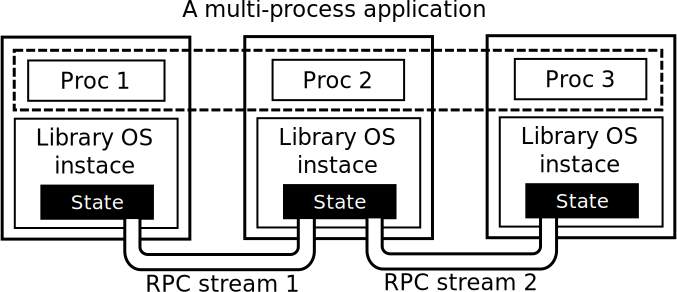
\includegraphics[width=4in]{graphene/figures/concept.pdf}
\caption[Multi-process support model of \sysname{} \libos{}]
{Multi-process support model of \sysname{} \libos{}. For each process of an application, a \libos{} instance will serve system calls and keep local OS states. States of multi-process abstractions are shared by coordinating over host-provided RPC streams, creating an illusion of running in single OS for the application.}
%\vspace{-.1in}
\label{fig:graphene:concept}
\end{figure}

{\bf \sysname{}} is a Linux-compatible library OS
to run legacy, unmodified Linux applications.
In \sysname{}, multiple \libos{} instances collaboratively implement
POSIX abstractions,
yet appear to the application
as a single, shared OS.
\sysname{} instances coordinate state using remote procedure calls (RPCs) over
host-provided byte streams (similar to pipes).
In a distributed POSIX implementation, placement of shared state and messaging complexity
are first-order performance concerns.
%We chose to shift implementation complexity into the library OS
%in order to uphold simple enforcement of security isolation in the host.
By coordinating shared states across \libos{} instances,
\sysname{} is able to create an illusion 
of running in a single OS
for multiple processes in an application (as figure~\ref{fig:graphene:concept}).
%Previous library OS designs ensured security isolation of independent applications,
%comparable to a VM, by keeping a relatively narrow host ABI.
%We selected the \sysname{}
%design because it strikes a unique balance between
%and robust, flexible security enforcement.
The \sysname{} design ensures security isolation of
mutually distrusting, multi-process
applications on the same host system.
Essential to this goal is
minimally expanding the host ABI to support multi-processing,
as well as leveraging RPCs as a natural point to mediate inter-\picoproc{} communication.
RPC coordination among \sysname{} instances can be dynamically disconnected, facilitating novel sandboxing
techniques.  For instance, we develop an Apache web server extension that, upon logging in a given user,
places the worker process's \libos{} in a sandbox with access to only that user's data.
We expect more nuanced degrees of trust are possible in future work.

\begin{comment}
The contributions of this paper are:
\begin{compactitem}
\item \sysname{}, a Linux library OS, which supports
  real-world, multi-process applications including a shell, web server,
  and compiler, which can be  efficiently checkpointed and migrated.
% \fixmetsai{We need to enable mulit-process checkpointing and migration}
% \daniela{the reviewers will be looking for that in the experiments section: "among hosts''}.
\item A framework for implementing multi-process APIs across cooperating library OS instances.
%\daniela{I would change to: "A thorough security analysis of \sysname{} isolation design'' You mention that you trust the reference momitor, so there is no security to
%be evaluated unless you guarantee the process is not vulnerable to exploits. We have not evaluated the security of the coordination design, only the isolation. To evaluate the security to the coordination design we have to look at possible race conditions and how they are dealt with.}
%\item Addressing additional challenges developing a robust Linux library OS, including copy-on-write fork.
\item A thorough evaluation of the overheads of \sysname{}.  Memory footprints are an order of magnitude
smaller than KVM, and several applications perform comparably to a Linux process.
\item A thorough analysis of \sysname{} security isolation.

%In the best case, the overhead of a large {\tt gcc} compilation on \sysname{} is only 3\%.

\end{compactitem}
\end{comment}

%\sysname{}'s design gives the user and system administrator a high degree of flexibility
%in isolating arbitrary groups of unmodified application processes,
%while upholding the efficiency and host compatibility benefits of recent library OSes.

%\fixmedp{After a complete draft is written, coalesce all goals and make sure they are addressed early on.  We are doing some scatter-shot motivation}


\papersection{Challenges for Partitioning with Enclaves}
\label{sec:background}
In this section, we will give a brief overview of \sgx{}, and discuss 
the key challenges developers face when trying to manually partition applications using a technology such as \sgx{}.
%discuss the programming models and threats to security of \sgx{} enclaves.

\papersubsection{Background on \intel{} \sgx{} Enclaves}

\intel{} \sgx{} ({\it Software Guard Extension})
is a set of new x86/x64 instructions
introduced in the \intel{} Skylake processor family.
Using \sgx{}, an 
application can designate part of its virtual memory as an {\em enclave}.
The CPU guarantees that the contents of the enclave never leave the CPU package unencrypted.
The CPU also measures the integrity of a binary loaded into the enclave, and offers remote attestation,
similar to a TPM\fixmedp{cite}.

%%% create a protected memory region, called an {\em enclave}, inside it's virtual memory,
%%% where it can load its security sensitive data with hardware-enforced isolation from the untrusted OS. 
%%% The processor with \sgx{}
%%% guarantees that any data loaded in enclave
%%% stays encrypted in the DRAM, by using a secret key deterministically derived from the application's cryptographic measurement and the CPU secret. 

\sgx{} is an appealing tool for protecting small amounts of highly-sensitive data or code, because it can defend 
against a malicious or compromsed OS, hypervisor, or even hardware peripheral.
For instance, \fixmedp{Foo} et al.~\fixmedp{cite that \sgx{} workshop paper} show how \sgx{} can be used
to build a trusted path from a video chat application to a GPU and network card, which maintains confidentiality and integrity of the
video stream, even if the OS is compromised.
Simlarly, because DRAM contents are encrypted, \sgx{} can resist cold-boot attacks~\cite{halderman09coldboot} or 
malicious peripheral devices~\cite{hudson15thunderstrike}.


%%% \sgx{} also proves the integrity of loaded binaries to remote trusted entities
%%% using mutual attestation based on a symmetric key generated from the measurements of communicating entities.
%%% \sgx{} usage model mostly involve the launched enclave mutually attesting the trusted host
%%% to obtain provisioning of security-sensitive information
%%% through a trusted channel. Such an execution model leverages resources such as CPU and DRAM from vulnerable untrusted \sgx{}-enabled hosts owned by cloud providers
%%% by extending the trust from
%%% the hosts owned and trusted by the clients or service providers.
%%% For instance, \sgx{} can isolate the decoder engine in an enclave
%%% after authenticating the customers to enforce Digital Right Management (DRM) even if the digital data is hosted on an untrusted cloud server.

%Use cases of \sgx{} mostly involve the launched enclave
%retrieving a cryptographically signed attestation from the processor,
%to exchange security critical information with remote servers through secured channels.
%The effect is equivalent to expanding the trusted space from remote servers
%to the local end, to harness local resources such as CPU and DRAM.

%One must note that \sgx{} only promises the integrity of application binaries
%initially loaded in enclaves.
%The gap between integrity of binaries and complete security has to be filled
%by ones who develop and approve the applications.
%More specifically, the clients are responsible of
%testing whether the applications contain any vulnerabilities
%that lead to information leak.
%To minimize the risk of leaving any flaws in the applications unintentionally,
%developers often tend to cut down the trusted computing base (TCB)
%of the applications. With smaller TCB, clients who launched the enclaves
%can more easily reason about the thoroughness of securing the execution.

%%% The key strength of \sgx{} enclaves over other software-based isolation framework such as
%%% {\em Flicker}, {\em Inktag} or {\em Virtual Ghost} is
%%% the ability to defend against attacks at the hardware level.
%%% These software-based solution often
%%% rely on a hypervisor below the OS to isolate the applications.
%%% If the hardware is attacked,
%%% the attackers may still bypass the software checkpoints,
%%% or directly steal confidential information from the DRAM.
%%% For \sgx{}, the only hardware included in the TCB is the CPU package,
%%% and in practice CPUs are believed to be hard to attack.
%%% Using techniques like cold-boot attacks~\cite{halderman09coldboot}
%%% to peek into DRAM content,
%%% or intruding the boot process using corrupted peripheral devices like Thuderstrike~\cite{hudson15thunderstrike}
%%% will affect any software-based isolation, but not \sgx{} enclaves.

\paragraph{Non-Partitioned Applications.}
One approach to using \sgx{} is to run an entire application in the enclave.
This is exemplified by Haven~\cite{baumann14haven}, which runs a \win{} application and all supporting libraries
on top of a {\em library OS}.  This approach is illustrated on the left side of Figure~\ref{fig:libosvssdk}.
The library OS approach does not require any application changes, but bloats the TCB \fixmedp{Rough number of how big Haven is}.
By pulling millions of lines of extraneous code into an enclave, there is a significantly increased risk 
of vulnerabilities that disclose
sensitive data, such as Heartbleed~\fixmedp{cite}.
The library OS approach is useful in its simplicity of deployment and can provide practical benefits, 
such as protecting an application from an untrusted cloud hypervisor.

\begin{figure}[t!]
\centering
\includegraphics[width=\linewidth]{figures/libosvssdk.pdf}
\footnotesize
\vspace{-0.2in}
\caption{
Comparison between the libOS-based model (e.g., Haven)
and the partitioned model for programing applications in enclaves.
Green (light) boxes are trusted components and red (dark) boxes are untrusted.
The libOS-based model yields a larger TCB in the enclave,
while the partitioned model requires developers to be responsible for determining the untrusted interface at the enclave boundary.
}
\label{fig:libosvssdk}
\end{figure}


This paper focuses on a second usage model for enclaves, where the application is partitioned into
untrusted and one or more trusted components (right side of Figure~\ref{fig:libosvssdk}).
Sensitive data and computation are placed inside of enclaves.  This approach requires the developer to
identify sensitive code and data; design and harden an interface between trusted and untrusted components; 
modify the application source; and reason about potential information flows at the enclave boundary.
This effort can be non-trivial and subtle, but for application developers motivated by interests such as 
regulatory compliance or competitive advantage in business, the additional effort can yield a much smaller trusted computing
base (TCB), and thus a reduced attack surface.
A key goal of \sysname{} is to minimize the developer's effort to partition an application---both in lines of 
code changed, and in leveraging language analysis to reason about narrow points in the application's data and control flow.


%To achieve smaller TCB, the software development kit of \sgx{}
%intends to encourage developers to partition the applications and
%keep only security sensitive components in the enclaves.
%Such an intention is exactly contradicted by the trust model of \haven{},
%which must trust the loaded application as a whole.
%Except for the cases in which the whole applications must be secured,
%\haven{} actually downgrades the trustworthiness of enclaves.
%Figure~\ref{fig:libosvssdk} shows the comparison of the two models.

%%% In prior works using \sgx{} enclaves to secure applications,
%%% developers choose between two different programing models: the {\em library-OS-based} and the {\em partitioned} model (as shown in Figure~\ref{fig:libosvssdk}).
%%% In the libOS-based model, developers run the whole standalone,
%%% legacy application inside the enclave, using library OS such as {\em Haven} or {\em Graphene libOS} to facilitate the rich OS features.
%%% The main benefit of using library OS is that developers only have to employ minimal efforts to port any existing application.
%%% Even when designing new applications, developers bear no responsibility
%%% of identifying and reasoning about
%%% the security sensitive part of the application.

%%% However, when using libOS-based model, a sophisticated legacy application
%%% will yield huge trusted computing base (TCB) in the enclave,
%%% aggravating the risk of leaking information through vulnerabilities inside the enclave.
%%% Known bugs such as {\em the heart-bleeding bug} has shown that
%%% running security sensitive code like an encryption engine, and management code such as heart-beating service in the same address space
%%% can cause vulnerabilities that compromise the security by leaking the encryption key.
%%% As a result, using a partitioned model, developers can isolate only the most security sensitive components in an enclave,
%%% and leave the remaining code outside to minimize the TCB.

%%% Developers have to define the {\em untrusted interface} 
%%% to allow parts of a partitioned applications to interact.
%%% The untrusted interface is used either by the the untrusted components
%%% to trigger execution of the isolated components,
%%% or by isolated components to use untrusted rich OS features, such as networking for provisioning and sending the execution output to the remote hosts.
%%% Unlike the libOS approach that has a fixed untrusted interface (for different applications) at their interaction boundary with the OS,
%%% the width of untrusted interface for a partitioned application is up to developers' design.
%%% The \intel{} SDK for \sgx{} supports a set of syntaxes to specify the type and direction of flow for parameters of the untrusted interface, and enforces primitive
%%% type-checking of incoming values on transition to enclave.

%%% The trade-off between the libOS-based and partition model is based 
%%% on ease of development, the width of untrusted interface,
%%% and size of TCB.
%%% The benefit of the libOS-based model is that developers can save the effort
%%% of determining what to execute in the enclave,
%%% and whether the execution is safe,
%%% because the whole application is wrapped in the enclave.
%%% However, the risk of having vulnerabilities in the applications
%%% is not reduced, but in fact amplified due to the addition of
%%% the library OS (e.g., the Haven binary yields around a few hundred MBs) to TCB.
%%% On the other hand, if the developers are willing to spend effort on carefully identifying the untrusted interface and re-designing their application around this interface, the partitioned model can improve security guarantees by minimizing the attack vectors.

%%% The goal of \sysname{} is to provide the benefits of both models.
%%% \sysname{} support a partitioned model
%%% for developers to isolate security-sensitive part of a \java{} application in enclave,
%%% and provide a language-based tool to automatically partition
%%% the minimal supporting classes to generate the enclave image.
%%% Even in the case where the isolated component need to frequently interact with the untrusted component or the OS,
%%% the language protection technique of information flow tracking
%%% guarantees that the secrets in the enclave are never leaked
%%% without the developers explicit consent. 

\paragraph{Side Channels and Denial-of-Service.}
In the current \sgx{} design, side channels are a signficant concern for either the library OS or partitioned model, and are out of the scope of this paper.
A controlled channel attack~\fixmedp{cite} can single step enclave execution by inducing page faults
in the enclave.  \sysname{} does not specifically defend against side channel attacks,
and we expect that any solution to this problem involves redesigning the division of labor in virtual
memory management for enclaves.

Similarly, there is no guarantee that a compromised application will ever enter
an enclave.  Denial-of-service attacks are out of scope for this paper.


\papersubsection{Challenges for Application Partitioning on \sgx{}}

\sgx{} provides useful building blocks for secure applications, but does not
absolve the programmer of any responsibility for reasoning about end-to-end security.
Bugs in the application or supporting libraries can still disclose sensitive data from an enclave,
and porting code into \sgx{} can be subtle.
This subsection outlines several pitfalls in partitioning an application for \sgx{}.

%%% \sgx{} enclaves provide strong isolation guarantee for applications,
%%% against the malicious or vulnerable application components, system stack,
%%% and hardware (except the CPU itself).
%%% However, the security guarantees of the \sgx{} enclave is dependent on whether the developers design perfect applications without exploitable vulnerabilities that may compromise the application's security.
%%% As the application developers are not perfect,
%%% even applications or components isolated in enclave can face threats to their security.
%%% As follows, we discuss a few potential threats
%%% to the enclave security,
%%% even under the assumption that the \sgx{} hardware is implemented as completely secure --- which can be another threat otherwise. 

%\fixmedp{I roughly want the rest of this section to have a problem, explanation, solution structure, with the overall theme being that this is subtle and we really need some analysis tools to get this right}

\paragraph{Writes outside of the enclave.}
\sgx{} allows code inside the enclave to read and write data structures 
outside of the enclave.  Thus, it is easy for a developer to inadvertently write
code that discloses a secret, say by using a library that memoizes intermediate results to the untrusted heap.
A fundamental requirement is that developers must be able to reason about (or assert)
what code can and can't access data {\em outside} of the enclave.
\fixmedp{Can we say anything about whether such tools exist before Civet?}

%\fixmedp{Do I recall correctly that you can easily write to data outside of the enclave?  If so, this seems like something easy to get wrong, especially 
%if a library memoizes intermediate results.  The developer needs to be able to tell 
%Unless I am full of shit, can we paragraph-ize this fixme?

\paragraph{Application vulnerabilities.} 
The major source of threats to enclave security is any internal vulnerabilities in the isolated components,
such as buffer overflows and other memory corruption attacks.
Moreover, although \sgx{} code integrity guarantees make enclaves resistant to code injection,
an attacker may still manipulate control flow using code-reuse attacks~\cite{code-reuse-attacks}.
Moreover, recent research ~\cite{hudata} show that even with perfect control flow integrity,
attackers can still manipulate the execution to leak the secrets through information flow.

Fundamentally, this argues for some combination of static analysis
and runtime monitoring of 
enclave code.  This is greatly simplified when the enclave code is written in higher-level languages
with properties 
%amenable to analysis.
%with type safety, memory safety, and other 
%that provide important 
%safety properties,
such as type safety or memory safety. %, thereby reducing the likelihood of these vulnerabilities.
Ideally, one would formally verify security properties of enclave code~\cite{moat}; this verification is significantly aided by using 
higher-level languages amenable to formal reasoning.
%Verification is significantly harder
%with C or x86 assembly.

%% \paragraph{Applications are not perfect} 
%% The \sgx{} hardware cannot prevent applications from copying secrets out of the enclave without limiting functionality.
%% The trusted isolated components can copy any sensitive data from the enclave to the unencrypted memory, and potentially leak the enclave secrets.
%% The primary risk in the isolated components
%% is often memory corruption vulnerabilities, such as buffer overflow,
%% %Because in enclave applications can access any part of out-of-enclave memory unrestrictedly,
%% prevalent in applications that are not implemented in type-safe languages.

%% The best known technique to prevent vulnerabilities is to model the applications and verify them using {\em formal verification}.
%% While Sinha et.al.,~\cite{moat} use formal verification to prove confidentiality of enclave programs, it is impractical to accurately model complex sophisticated applications.
%% As a result, in addition to formal verification, maintaining smallest TCB
%% in the isolated components is the most practical approach 
%% to ensure enclave security,
%% and is the main reason to choose partitioned programming model over
%% libOS-based model.


\begin{figure}[t!]
\centering
\includegraphics[width=\linewidth]{figures/partition.pdf}
\footnotesize
\vspace{-0.3in}
\caption{
Partitioning --- either manually or by automated tool ---
often causes wider boundary of partition than the actual security sensitivity boundary
due to (a) design granularity : {\tt secHelper} contains a {\tt send()} method that is not partitioned from the rest of the class by design.
The reasons of having the gap vary, for instance, 
that is less security sensitive, but due to the granularity it is not partitioned from the rest of the class or (b) better performance :  the less security sensitive {\tt logger} class is kept in the privileged level to service frequent method calls.
}
\label{fig:partition}
\end{figure}

%However, even if developers partition the applications and run only
%security sensitive components in the enclave,
%the developers may still leave some code irrelevant to
%enclave secrets inside the enclave.
%The reasons of having more-than-minimal TCB in enclaves
%are often that developers have to partition code in the granularity of source files or functions,
%or developers have to import more code to limit the width of interface and
%the frequency of interaction with the untrusted code.

\paragraph{Identifying ``pinch points''.}
Reasoning about where in a program to draw the line between 
trusted and untrusted code is subtle.
On one hand, the developer has an incentive to minimize the size of the 
API between the enclave and untrusted code, as well as an incentive to
minimize the total code in the enclave.  These goals can sometimes be at odds.
Each entry and exit to an enclave has a cost roughly comparable to a
process context switch\fixmedp{right?}; an easy way to reduce enclave entries and exits is to simply 
pull more code into the enclave, which increases the size of the TCB.

\fixmedp{I'm not sure how to explain Figure~\ref{fig:partition}, but it needs an explanation.}

Fundamentally, the art of paritioning an application is to find a ``pinch point'' or
``narrow waist'' in the application, where there is a natural point to insert an API and 
security checks.  This is indeed as much art as science, often done manually by experts\fixmedp{any more supporting evidence or cites?}.
It is unlikely that the average developer will successfully navigate this design process without analysis tools, such as \fixmedp{examples?},
to help identify these natural division points.


%% Experts can use a manual partitioning technique to achieve smallest TCB for the isolated components compared to automated tools.
%% However, the manual partitioning costs a lot of effort,
%% and rare expertise, lack of which can cause larger TCB.

%% Neither manual nor automated partitioning is perfect:
%% the resulted boundary of partitioning often has a gap from the actual boundary of security sensitivity (as shown in figure~\ref{fig:partition}),
%% leaving more code in the privileged level
%% than what's actually needed.
%% Having the gap between the ideal and resulted boundary
%% is mostly inevitable, due to multiple reasons.
%% One common reason is the granularity of partitioning,
%% which can vary from a binary file, a component, a source file,
%% a class, a method (a function) to a line of code.
%% Another reason is that a component or a method may be too frequently called
%% by the security sensitive code,
%% laying the boundary between the component or method from the security sensitive side may bring too much overhead or risk,
%% because the execution crosses the boundary too often.
%% Therefore, developers often will balance among the effort of partitioning,
%% risk or cost of communicating between different partitions,
%% and minimizing the TCB in the security sensitive parts.

\fixmedp{Maybe move the commented paragraph below down into the design section?  I'd like to downplay the plugs for our work here, and instead fulfill these promises later}
%% \sysname{} automates partitioning of applications,
%% based on the boundary at the classes which the developers marked
%% as the interfaces of the enclave.
%% Only the classes that are depended by the marked classes
%% will be included in the enclaves,
%% to minimize the TCB.
%% Although not all classes pulled into the enclaves
%% are necessarily security sensitive,
%% the enclaves are protected from the potential vulnerabilities in those classes,
%% by the security guarantees of \java{} language,
%% and the information flow tracking in \sysname{}.

%Another threat to \sgx{} is the vulnerability of the 
%security sensitive code running in the Enclave. The 
%main guarantee of \sgx{} to isolate the secure data 
%from other components and privileged OS is undermined 
%if the Enclave code can be tricked to leak the 
%security sensitive data to the attacker. Executing 
%buggy code in \sgx{} enclave can inadvertently leak 
%information if the attacker can exploit memory-safety 
%vulnerabilities like buffer overflow and dangling 
%pointers.  

% Cumbersome and approximation to partition code
%The developers have to manually partition their code 
%into security sensitive and insensitive part. If this 
%partitioning is done by a novice developer, some of 
%the security insensitive parts of the application can 
%end up in the security sensitive part, increasing the 
%Trusted Computing Base(TCB). Moreover, the 
%partitioning of code is not straightforward, which 
%can also contribute to a less stricter TCB. The bigger the TCB, the more %vulnerable is the Enclave code to attacks.

% Buggy Code leads to inadvertant information leakage


% \sgx{} code only Integrity protected not confidential
%Moreover, \sgx{} only protects the integrity of the enclave code. The security critical part of the application is stored in plaintext while the secret data is provisioned securely after attestation. However, \sgx{} does not protect the confidentiality of enclave application code which may be executing a secret algorithm. \fixmebj{Talk more about the problem motivating security tag preservation.}
%\sgx{} can natively guarantee either code integrity or
%code confidentiality (as part of the enclave data), but not both.
%If application code is included in the enclave measurement and
%verified by the hardware,
%the code must stay in plaintext as part of the enclave image.
%If any code is stored or provisioned in encrypted forms,
%the application or infrastructure in enclave must dynamically load
%the code after decryption.
%Supporting dynamic loading makes enclaves open to code injection
%if the applications have exploitable vulnerabilities.

\paragraph{Code Integrity {\em and} Confidentiality.} 
The hardware-level \sgx{} code integrity mechanism is based on a cryptographic
signature of a static binary in plaintext.
If any application dynamically loads any code after the enclave's initial measurement,
the initial application must be trusted to attest the loaded code.
The subtle tension is that there is no way to protect the confidentiality of
a secret algorithm, except by dynamically loading an encrypted binary.
Dynamically loading code increases the risk of code injection attacks and other control flow compromises.

Any application partitioning solution that protects sensitive algorithms
must have a robust dynamic loader that can measure encrypted libraries or classes.
\sysname{} includes a loader that can measure encrypted class files,
provisioned from a trusted host.

%% \sgx{} enclaves require code integrity in the isolated applications.
%% If the code integrity is not maintained, adversaries can corrupt the enclave code to
%% force the applications to leak the information provisioned from the remote,
%% trusted hosts.
%% \sgx{} hardware only guarantees
%% the integrity of the code initially loaded into the enclaves.
%% However, if an application choose to dynamically
%% load any code after the enclave starts,
%% the application is responsible for the integrity of the code loaded.
%% The fact that dynamic loading of applications, libraries or components
%% is a feature that can potentially make enclaves vulnerable and open to code injection,
%% raises concerns against supporting managed languages in the enclaves.

%% On the other hand, code confidentiality can be a desirable feature,
%% for application developers who prefer keeping the secret sauce of their algorithms concealed.
%% To enable the feature of code confidentiality in enclaves, the protected code must be dynamically loaded into the enclave,
%% because the \sgx{} hardware only accept
%% the initial loaded code to be in plaintext.
%% \sysname{} provides both code integrity and confidentiality by verifying
%% every classes dynamically loaded into the enclaves,
%% and allows loading classes provisioned from trusted hosts.


%% In general \sgx{} enclaves are prone to having side channels, such as timing channels. Because \sgx{} relies on the untrusted OS for paging,
%% an enclave will always leak page fault addresses, except the lower 12 bits (offsets in pages).
%% Such a leakage gives the untrusted OS to amplify the side channels,
%% by forcing page faults on every instruction or memory access.
%% This so-called {\em Controlled Channel Attack} is common to all applications who use \sgx{} protection, regardless of the programming models.
%% \sysname{} does not specifically defend against side channel attacks.

%% \paragraph{Denial-Of-Service Attacks}
%% \sgx{} is not designed to be safe against denial-of-service attacks.
%% Because the untrusted OS still controls the host resources,
%% there are countless ways to prevent an enclave from making progress.
%% For example, the OS can simply starve the enclaves by
%% never scheduling CPU, memory or other resources to the enclaves.
%% \sysname{} does not specifically defend against denial-of-service attacks.

\paragraph{Discussion.}  This
section has outlined several pitfalls for developers of partitioned applications.
These common pitfalls render the hardware protections of \sgx{} useless.
Language-level analysis can automate error-prone reasoning in the best case, or, in the worst case, 
can at least offer invaluable guidance to the developer.  For \sgx{}-style
hardware to be useful to a wide array of developers, developers need language-level
tools that can also factor in hardware-level protection mechanisms.



%- Motivate the problem.
%- List all attack vectors
%- How can JAVA help?




















































































\section{Coordinating Guest OS States}
\label{sec:libos:namespaces}

%\fixmedp{RF: what are the few, powerful mechanisms?  Expect that there are many cases 
%with shared state; re-read this to see if it is clear how to generalize the approach}

%Recent library OS designs focus on single-process applications,
%which move a substantial portion of the OS APIs and state used by the application into the \libos{}.

%A key contribution of the \graphene{} 
%design is robust and flexible support for multi-process applications.
A multi-process application executes on \graphene{} 
with the abstraction that all of its processes runs on a single OS.
Each \thelibos{} instance services \linuxapis{}
from its local state whenever possible.
However, whenever a \thelibos{} instance must share a \libos{} state with other instances,
\thelibos{} has to coordinate the state across \picoprocs{}
via a RPC stream.
Within a sandbox, multiple \picoprocs{} 
can securely coordinate shared states of multi-process abstractions, including process IDs, exit notification and signaling, 
System V IPC mechanisms (message queues and semaphores), shared file system states, and shared file descriptor states (Table~\ref{tab:libos:multiproc}).
%Similar to previous \liboses{}~\cite{porter11drawbridge,baumann13bascule}, 
%\graphene{} uses the host file system; 
%the \libos{} implements file handles and translates between POSIX and the host ABI.
%Identifying the best division of labor for a \libos{} file system is 
%left for future work.
\thelibos{} contains a coordination framework
with several building blocks for implementing a shared multi-process abstraction.

\begin{table}
\footnotesize
\centering
\begin{tabular}{|p{.16\textwidth}|p{.20\textwidth}|p{.55\textwidth}|}
\hline
{\bf Ab\-strac\-tion} & {\bf Shared State} & {\bf Coordination Strategy} \\
\hline
Fork & 
\raggedright
PID namespace & Batch allocations of PIDs, children generally created using local state at parent.  \\
\hline
Signaling & PID mapping & Local signals call handler; remote signal delivery by RPC.  Cache mapping of PID to \picoproc{} ID. \\
\hline
\raggedright
Exit notification & 
\raggedright
Process status  & Exiting processes issue an RPC, or one synthesized if child becomes unavailable.  The {\tt wait} system call blocks until notification received by IPC helper. \\
\hline
{\tt /proc/[pid]} & Process metadata & Read over RPC.  \\
\hline
Message Queues & 
\raggedright
Key mapping \newline
Queued messages &
Mappings managed by a leader, contents stored in various \picoprocs{}.  When possible, send messages asynchronously, and migrate queues to the consumer.\\
\hline
Semaphores & 
\raggedright
Key mapping \newline
Semaphore count &
Mappings managed by leader, migrate ownership to \picoproc{} most frequently acquiring the semaphore. \\
\hline
\raggedright
File System & 
\raggedright
File truncate sizes \newline
Deleted files \newline
FIFO \& domain sockets \newline
Symbolic links
& No coordination; completely relying on \thehostabi{}; creating special files in the host to represent symbolic links. \\
\hline
\raggedright
Shared File Descriptors & 
\raggedright
Seek pointers & Mappings managed by parent, migrate ownership to \picoproc{} most frequently accessing the file descriptors. \\
\hline
\end{tabular}
\caption[Multi-process abstractions implemented in sysname{}]
{Multi-process abstractions implemented in \graphene{}, coordinated state, and implementation strategies.}
\label{tab:libos:multiproc}
\end{table}


%% Outline

% Basic idea of what we are doing
% Building blocks
% Implemented abstractions and examples (table)
%% Why not shared FDs?
% Optimizations/insights
% Why different from microkernels?



As an example of balancing security isolation and coordination APIs,
consider functionality that use the process ID namespace,
such as UNIX signaling or exit notification (e.g., {\tt waitpid()}).
In \graphene{}, the process ID namespace, 
as well as signaling and related system calls,
are implemented inside \thelibos{}.
A process can signal itself by having the \libos{} directly call the handler function.
When \picoprocs{} are in the same sandbox, they coordinate
to implement a consistent, shared process ID namespace,
as well as to send and receive signals amongst themselves.
Cross-process signals are implemented as RPCs
over kernel-managed streams.
When \picoprocs{} are in separate sandboxes,
they do not share a PID namespace, and cannot send signals to each other.
The reference monitor ensures that IPC abstractions, such as signaling,
cannot escape a sandbox by preventing the creation of kernel-level streams
across sandboxes.



%Figure~\ref{fig:libos:sandbox} illustrates several sandboxes with \picoprocs{}
%collaborating to implement a process ID namespace.  
%Because this namespace is a guest-level abstraction,
%different sandboxes can have overlapping process IDs, and
%cannot signal each other.
%If the connection between the two \picoprocs{} on the right of the figure
%is severed by subdividing the sandbox,
%the processes will become inaccessible to each other
%and each newly isolated library OS will treat the event as a process termination.
%%\fixmedp{See if we can get a better figure}

%dp:  Seems redundant, probably imported from S2
\begin{comment}
Within a sandbox, each library OS tracks the PIDs of other \picoprocs{}.
As children are created, each library OS updates its own replica of the 
process tree, with annotations for which host-level connection corresponds
to the remote process.  
If a \picoproc{} signals itself, the signal system call simply calls the 
appropriate signal handling function in the application. 
If a \picoproc{} signals another \picoproc{},
the signal essentially becomes an asynchronous remote procedure call
from the sending library OS to the receiving library OS.
Note that this is all transparent to the unmodified application.
Section~\ref{sec:graphene:namespaces} describes these library OS-internal
coordination mechanisms in more detail.
The current \graphene{} prototype supports 
a range of coordination abstractions, including signaling, 
exit notification, System V message queues, thread identifiers and groups, sessions,
and the process tree.
We believe this sample is sufficiently representative that
remaining tail of Linux IPC abstractions could be easily added.

The reference monitor ensures security isolation
simply by preventing \picoprocs{} in different sandboxes from 
sharing host-level streams.
We adopted this approach to maximize dynamic sandboxing flexibility,
rather than, say, attempt to multiplex one single library OS instance across multiple processes.
\end{comment}


A driving design insight is that the common case
for coordination is among pairs of processes.
Examples include a parent waiting on a child to exit, 
one process signaling another, or a single producer and single consumer
sharing a message queue.
Thus, \graphene{} optimizes for the common case of pairwise coordination,
reducing the overhead of replicating data (see Section~\ref{sec:libos:namespaces:lessons}).


%The rest of this section describes our coordination framework, 
%beginning with the coordination building blocks,
%and then explains the implementation of several multi-process abstractions.
%We conclude with lessons learned from optimizing  multi-process performance.

Although a straightforward implementation worked, tuning the performance was the most challenging aspect of the coordination framework. 
This section summarizes the lessons learned during the development of \graphene{}, from optimizing the coordination of various multi-process abstractions.
This section then
presents the design and driving insights of the coordination framework,
followed by representative examples 
and a discussion of failure recovery.

\subsection{Building blocks}
\label{sec:libos:namespaces:building-blocks}

The general problem underlying each of the coordinated \libos{} states is 
the coordination of {\bf namespaces}.  In other words, coordination between \picoprocs{} need 
a consistent mapping of names, such as process IDs or System V IPC resource keys, 
to the \picoproc{} implementing that particular item.  
Because many multi-process abstractions in Linux can also be used by single-process applications,
a key design goal is to seamlessly transition between single-process uses, serviced 
entirely from local \libos{} state, and multi-process cases, which coordinate shared abstractions over RPC.

%Picoprocesses then implement abstractions such as signals
%by issuing a remote procedure call (RPC) to the appropriate \picoproc{}.

\thelibos{} creates an {\bf IPC helper} thread within each \picoproc{}
to respond to coordination messages from other \picoprocs{}. 
%within the sandbox. %, using these broadcast and point-to-point streams.
An IPC helper
maintains a list of point-to-point RPC streams, and indefinitely waits for incoming messages.
For each multi-process abstractions coordinated over RPC,
\thelibos{} defines a protocol for formating the header of each message,
and determining the callback function for processing the message.
GNU Hurd~\cite{hurd} has a similar helper thread to implement signaling among a process's parent and
immediate children;
\graphene{} generalizes this design to share a broader range of multi-process abstractions among any \picoprocs{}.
IPC helpers in necessary 
in \thelibos{} to serve remote messages and receive responses atomically,
so one IPC helpers must be created in each \picoproc{}
after the application spawned its first child process.
To avoid deadlock among application threads and the IPC helper thread, 
an application thread may not both hold locks required by the helper thread to service an RPC request
and block on an RPC response from another \picoproc{}.
All RPC requests are handled from local state and do not issue recursive RPC messages.% \fixmedp{Check this}

Within a sandbox, all IPC helper threads exchange messages using a
combination of
a {\bf broadcast stream} for global coordination,
and {\bf point-to-point} RPC streams for pairwise interactions, 
minimizing overhead for unrelated operations.
The broadcast stream is created for the \picoproc{} as part of initialization.
Unlike other byte-granularity streams, the broadcast stream sends data at the granularity of messages,
to simplify the handling of concurrent writes to the stream.
Point-to-point RPC streams include the streams between parent and child processes established during \palcall{ProcessCreate},
and RPC streams created through connecting to a RPC server
identified by its URI.
% simply byte streams between two \picoprocs{};
%two processes may establish a point-to-point stream by passing handles through 
%an intermediate stream or over the broadcast stream.
%The handle-passing ABI is discussed further in Section~\ref{sec:graphene:impl}.
Because of the security isolation in the host,
only \picoprocs{} in the same sandbox can connect to each other through RPC.
%The broadcast stream is primarily used for failure 
%recovery (\S\ref{sec:namespaces:failurerecovery}); 
%Mmost operations use point-to-point streams to minimize overheads.
If a \picoproc{} leaves a sandbox to create a new one,
its broadcast stream is shutdown and replaced
with a new one, connected only between the \picoproc{} and any children created in the
new sandbox.

Because message exchange over the broadcast stream does not scale well,
we reduce the use of the broadcast stream to the minimum.
One occasion of using the broadcast stream is
{\bf \picoproc{} identifier allocation}.
Because each \picoproc{} needs an unique identifier to be recognized as a source or a destination of RPC messages, \thelibos{} generates a random number as the identifier of each \picoproc{} and confirms the uniqueness of the identifier over the broadcast stream.
Another occasion of using the broadcast stream
is {\bf leader recovery}, which happens when a namespace leader unexpectedly crashes
during coordination. The implementation of leader recovery will be discussed in Section~\ref{sec:libos:namespaces:details}.


For each namespace (e.g., process IDs, System V IPC resource keys), \thelibos{} elects one of the \picoprocs{} in a sandbox to serves as the {\bf leader}.
A leader is responsible for
managing and memorizing the allocation of identifiers or resources in a namespace,
in behave of all other \picoprocs{}.
For a namespace like the process ID namespace,
the leader subdivides the namespace for each \picoproc{} to reduce the RPC cost of allocation.
For example, the leader might allocate 50 process IDs to a \picoproc{} which intends to clone a new thread or process.
The \picoproc{} who receives the 50 process IDs becomes the {\bf owner},
and can further assign the process IDs
to children without involving the leader.
For a given identifier, the owner is the serialization point for all updates,
ensuring serializability and consistency for that resource.
%%% the leader's IPC helper has the added responsibility of coordinating 
%%% global state (name allocations).
%%% Our design minimizes the role of the leader, instead distributing responsibility 
%%% to specific \picoprocs{} when practical.  
%%% If the leader crashes, 
%%% a new leader can be elected. The detail of leadership recovery is discussed in
%%% Section~\ref{sec:namespaces:leader}. 
%More detailed discussion of the \graphene{}-internal
%RPC protocol is omitted for space;
%but it 
%consists of 30 message types which 
%encode both state replication and RPC 
%messages.

\subsection{Examples and discussion}
\label{sec:libos:namespaces:details}

%This subsection describes \libos{} coordination by example.
%\vspace{5pt}
\paragraph{Signals and exit notification.}
{\tt libLinux} implements signals
in various ways according to the causes of sigals.
For signals triggered by hardware exceptions (e.g., \code{SIGSEGV}),
\thelibos{} uses the hardware exception upcalls
in \thehostabi{}.
If a signal is sent from one of the processes for IPC purposes (e.g., \code{SIGUSR1}),
\thelibos{} exchanges RPC messages between \picoprocs{} to deliver the signal to the destination \picoproc{}.
%mplemented using a combination of 
%{\tt sigaction} data structures %adapted from Linux
%to track signal masks and pending signals;
%\pal{}-provided hardware exception upcalls (e.g., for {\tt SIGSEGV});
%and  RPCs for cross-\picoproc{} signals (e.g., for  {\tt SIGUSR1}).
If a process simply signals itself, {\tt libLinux} interrupts the targeted threads inside the process
and uses internal data structures
to call the appropriate user signal handler.
%this section describes how this local model is extended with RPCs for remote PIDs.
%For cross-process signals, we use the namespace coordination mechanism.
\thelibos{} implements all three of Linux's signaling namespaces:
process, process group, and thread IDs.
If a signal is sent for a process or a process group,
every threads within the process or the process group receives a copy of the signal,
even if the threads belong to different \picoprocs{}.


Exit notification in Linux is based on the same mechanism as signaling.
When a process exits, normally a \code{SIGCHLD} signal
is delivered from the child process to its parent,
to unblock the parent who might be waiting for exit notification using \syscall{wait} or \syscall{waitpid}.
Exit notification is always coordinated over RPC streams
between parent and child \picoprocs{}.



\begin{figure}
\centering
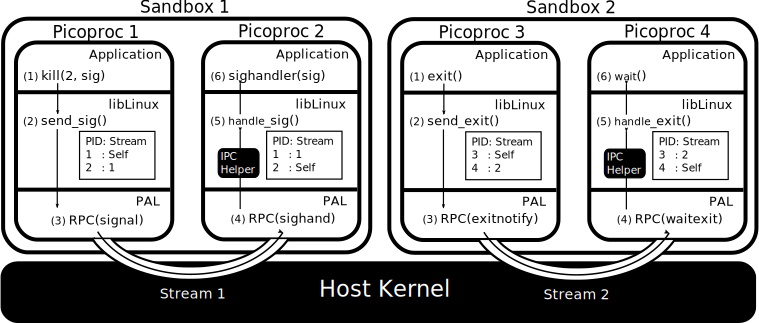
\includegraphics[width=\linewidth]{coordination.pdf}
\caption{Two pairs of \graphene{} \picoprocs{} in different sandboxes 
coordinate signaling and process ID management.
The location of each PID is tracked in {\tt libLinux}; Picoprocess 1 signals
\picoproc{} 2 by sending a signal RPC over stream 1,
and the signal is ultimately delivered using a 
library implementation of the {\tt sigaction} interface. Picoprocess 4 
waits on an {\tt exitnotify} RPC from  \picoproc{} 3 over stream 2. }
\label{fig:libos:coordination}
\end{figure}


Figure~\ref{fig:libos:coordination} illustrates two sandboxes with \picoprocs{}
collaborating to implement 
signaling and exit notification
within their own
process ID (PID) namespaces.  
Because process IDs and signals are \libos{} abstractions,
\picoprocs{} in 
each sandbox can have overlapping process IDs, and
cannot signal each other.
The host reference monitor ensures that
picoprocesses in different sandboxes cannot 
exchange RPC messages or otherwise communicate.
%If the connection between \picoprocs{} 1 and 2 is severed by subdividing the sandbox,
%the processes will become inaccessible to each other
%and each newly isolated library OS will treat the event as a process termination.



If \picoproc{} 1 (PID 1) sends a \code{SIGUSR1} to \picoproc{} 2 (PID 2), illustrated in Figure~\ref{fig:libos:coordination},
a \syscall{kill} call to \thelibos{} will check its cached mapping of PIDs to 
point-to-point streams.
If \thelibos{} cannot find a mapping, it may begin by sending a query to the leader
to find the owner of PID 2,
and then establish a coordination stream to \picoproc{} 2.
%The leader may also pass a point-to-point coordination stream handle.
Once this stream is established, \picoproc{} 1 can send a  
signal RPC to \picoproc{} 2 (PID 2).
When \picoproc{} 2 receives this RPC, 
\thelibos{} will then query its local \code{sigaction} 
structure and mark \code{SIGUSR1} as pending.
The next time \picoproc{} 2 calls \syscall{kill},
the \code{SIGUSR1} handler will be called upon return. Also in Figure~\ref{fig:libos:coordination}, \picoproc{} 4 (PID 2) waits on 
\picoproc{} 3 termination (in the same sandbox with PID 1). When \picoproc{} 3 terminates, it invokes the library implementation of exit, which issues
an \code{exitnotify} RPC to \picoproc{} 4.
%In this example, \picoprocs{} in different sandboxes have the same PID number, but this does not cause conflict as they are isolated and can only communicate with processes in the same sandbox.

%%% Using a helper thread alongside each process to asynchro-
%%% nously handle signaling
%%% is common in many \microkernel{}-based OSes such as GNU Hurd~\cite{hurd}.
%%% GNU Hurd also maintains local mappings of PIDs and RPC ports for inter-process messaging.
%%% However, PID namespace in GNU Hurd is only tracked between the parents/children, so signaling cannot be transferred between arbitrary processes.
%%% \graphene{} handles PID namespace with global consistency inside a sandbox,
%%% but requires no intensive RPCs to any centralized service.   

The signaling semantics of \thelibos{} closely match the Linux behavior, which
delivers signals upon returning from a system call
or an exception handler.
Each process and thread have \code{sigaction} structures from the Linux source 
that implement the
POSIX specification, including handler functions, as well as masking signals and
reentrant behavior.
\thelibos{} does not modify \libc{}'s signal handling code. % is unmodified on \graphene{}.
%We extend the \pal{} with ABIs for explicit upcalls on certain hardware exceptions, such
%as divide-by-zero or segmentation faults.
%Signals from other processes, such as {\tt SIGUSR1}, are generally delivered upon 
%return from a call into {\tt libLinux}; 
If an application has a signal pending for too long,
e.g., the application is in a CPU-intensive loop, {\tt libLinux} can use \palcall{ThreadInterrupt} in \thehostabi{} to interrupt the running thread. 


% Daniela Oliveira commented. old caption for coordination
%\caption{\graphene{} namespace coordination example.  
 % Two applications and {\tt libLinux} instances
 % coordinate signaling and process ID management.
 % The location of each PID is tracked in {\tt libLinux};
 % a signal message is sent over a host stream
 % using the {\tt action} message, 
 % and the signal is ultimately delivered using a 
 % library implementation of the {\tt sigaction} interface.
%}


\begin{comment}
\graphene{} internally indexes point-to-point handles using PIDs.
In order to facilitate reallocation of PIDs without global coordination, 
\graphene{}-internal PIDs also include a {\em generation number},
allowing \picoprocs{} to lazily detect reuse similar to generation numbers 
for inodes in NFS~\cite{sandberg85nfs}.
\end{comment}

\paragraph{System V IPC.} System V IPC
maps an application-specified key onto a unique identifier.
All System V IPC abstractions, including message queues and semaphores,
are then referenced by a resource ID, which is arbitrarily allocated.
Similar to process IDs, 
%In order to service IPC requests, including identifier creation, from local state,
the leader divides the namespace of resource IDs among the \picoprocs{},
so that any \picoproc{}
can allocate a resource ID from local state instead of involving the leader. %a pre-allocated range.
Unlike the resouce IDs, System V IPC keys must be centrally managed
by the leader,
since an application might autonomously assign System V IPC keys to its processes.
%The leader also dynamically allocates keys to \picoprocs{}.
Global coordination is required to ensure that the same key maps to the same resource ID;
the leader caches this information, but the owner of the resource ID 
makes the definitive decision about whether a ID mapping is still valid.
A key which does not have a valid mapping can be assigned to a resource ID by any \picoproc{} to allocate a {\em private} IPC resource.



\paragraph{System V IPC message queues.} In \graphene{}, the owner of a queue ID is responsible for 
storing the messages written to a System V IPC message queue.
To ensure the serializability and consistency of all messages, any delivery and reception of messages must go through the owner.  
In the initial implementation of \thelibos{}, sending or receiving messages remotely over a RPC stream
orders of magnitude slower than accessing a local message queue.
This observation led to two essential optimizations.  
First, sending to a remote
message queue was made asynchronous.  In the common case, the sender can simply assume 
the send succeeded, as the existence and location of the queue have already been determined.
The only risk of failure arises when another process deletes the queue.
When a queue is deleted, the owner sends a deletion notification to all other \picoprocs{}
that previously accessed the queue.
If a pending message was sent concurrently with the deletion notification 
(i.e., there is an application-level race condition), 
the message is treated as if it were sent after the deletion and thus dropped.
The second optimization migrates queue ownership from the producer to the consumer,
which must read queue contents synchronously.

%\fixmedp{bill: it is referenced in the Semaphores section, but here there isn't any talk about migrating msg queues to the most active \picoproc{}. also, the section starts with ``two essential optimizations. First \ldots'', but there isn't a second. is queue ownership migration the second?}

Because non-concurrent processes can share a message queue,
our implementation also uses a common file naming scheme to serialize message queues to disk.
If a \picoproc{} which owns a message queue exits, 
any pending messages are serialized to a file in the host,
and the receiving process may regain the ownership of the message queue later from the leader and recover the serialized messages.
%In order to prevent happens-before violations in case of failure, 
%message queues may be checkpointed more aggressively.


%\paragraph{Failure Recovery.}
%\label{sec:namespaces:failurerecovery}
%The \graphene{} coordination protocols are designed such that the leader does not store any unrecoverable information---the leader
%only caches the current name allocations.
%Because we assume that \picoprocs{} within a sandbox trust each other, 
%a new leader can simply broadcast a request to 
%recreate the current name allocations.  
%If the leader crashes, a simple leader election protocol is sufficient, e.g., picking the smallest live PID.

%\daniela{I wonder if the remainder of this section should be part of implementation details(section 5)}

\paragraph{System V IPC semaphores.} System V IPC semaphores 
follow a similar pattern to message queues.
Each semaphore is owned by a \picoproc{};
a semaphore can be directly accessed by its owner as a local state,
whereas other \picoprocs{} all have to access the semaphore through the owner over RPC.
Since a semaphore shares the same performance pattern as a message queue,
\thelibos{} applies the same optimization
of migrating the ownership of a semaphore
%, where ownership of a given semaphore is migrated
to the \picoproc{} that most frequently acquires the semaphore.
%If the owner of a semaphore exits, \graphene{} transfers ownership to the leader.  rather than serialize the semaphore to disk.
Another optimization of message queues, by making the updates asynchronous,
does not apply to semaphores,
because a participating \picoproc{} cannot proceed before successfully acquiring the semaphore. 
Most of the overhead in the Apache benchmark (see Section~\ref{sec:eval:graphene}) is attributable to semaphore overheads.
%and, in ongoing work, we will likely optimize this by 
%either expanding the host ABI to share synchronization primitives within a sandbox,
%using shared memory to reduce semaphore latency.

\paragraph{Shared file descriptors.}
The seek pointer of each file descriptor is implemented as a \libos{} abstraction;
when reading or writing to a host file,
\thehostabi{} always obtains an absolute pointer from the beginning of the file.
Although most applications
do not share the seek pointer of an inherited file descriptor among processes,
the {\tt clone} system call
can can be called with the {\tt CLONE\_FILES} flag
and create a process
which shares the whole file descriptor table with its parent.
%The default Linux behavior is that children copy the open handles and file seek cursors,
%but subsequent cursor movements are not shared between parent and child.
%Shared file descriptor table can be requested by passing the {\tt CLONE\_FILES} flag to the {\tt clone} system call.
%Any new file descriptor opened in a shared table will be visible by every process cloned in this way, as well as subsequent cursor update.
%None of our target applications have required a shared seek cursor, and it is not currently implemented,
%but would be a straightforward extension to current RPC mechanisms.
%We expect that the current RPC mechanisms could easily be extended to synchronize a seek pointer among \picoprocs{}.
To share a file descriptor table among \picoprocs{},
one of \picoprocs{} (usually the oldest one)
must be the leader of the file descriptor table to manage all mappings
from file descriptors to the child \picoproc{} who owns the state of the file descriptors including the seek pointers.
Every updates to a seek pointer must goes through the owner of the file descriptor (not the leader).
The migration-based optimization for System V IPC message queues and semaphores is also effective for optimizing the performance of shared file descriptors. 

\paragraph{Shared file system states.}
A chroot file system in \thelibos{}
is restricted by \thehostabi{} to externalize any file system states.
Other shared file system states are implemented as \libos{} abstractions, and have to be coordinated among \picoprocs{}.
For example, a POSIX file system can contain special files such as a FIFO (first-in-first-out); a path bound to a UNIX domain socket;
a symbolic link; or a file system lock.
Implementation of these special files cannot
completely depend on \thehostabi{},
since the abstractions of \thehostabi{} contains only regular files and directories.

%Coordinating these states can be cause significant slowdown on regular file system operations, so we simply export the state in regular files on the host,
% and atomically update them by renaming.

A simple approach to coordinating file system states is to share a ``dummy'' host file.
For example,  \thelibos{} can store the target of a symbolic link
in a regular file on the chroot file system.
For a FIFO, a bounded UNIX domain socket, or a file system lock,
\thelibos{} can store a mapping to the corresponding RPC stream, or to the \picoproc{} which owns the abstraction.
By using the host file system as a less efficient but permanent coordination medium,
\thelibos{} can extend the coordination framework for sharing file system states.



\paragraph{Shared memory.} The \graphene{} architecture 
does not currently permit shared memory among \picoprocs{}.
This thesis expects that an extra \hostapi{} and the existing support for System V IPC coordination would be sufficient to implement this,
with the caveat that the host must be able to handle sandbox disconnection gracefully, perhaps converting the pages to copy-on-write.
Thus far \graphene{} have avoided the use of shared memory in \thelibos{},
both to maximize flexibility in placement of \picoprocs{}, potentially on an unconventional host (e.g., Intel SGX) or different physical machines.
and to keep all coordination requests explicit.
Shared memory may also be useful to reduce latency for RPC messaging among \picoprocs{} when 
all \picoprocs{} are on the same host.


%in \graphene{} are implemented by a simple producer-consumer model.
%%% Without blocking, the latency of an inter-process semaphore operation equals to a round-trip of RPC messages.
%%% We observed that IPC semaphores can benefit from the same optimization
%%% used by message queues,
%%% based on asynchronous sending.
%%% However, when non-concurrent processes share a semaphore, it does not worth serializing the semaphore state to disk.
%%% When the owner of a semaphore exits,
%%% the semaphore state will be migrated to the leader,
%%% if it has a non-zero counter.
%%% IPC semaphores are intensively used in Apache web servers with a multi-process model. 

 


\paragraph{Failure and disconnection tolerance.}  
\thelibos{} must tolerate disconnection between collaborating \picoprocs{},
either because of crashes or blocked RPC streams.  In general, \thelibos{} makes 
these disconnections isomorphic to a reasonable application behavior,
although there may be some edge cases that cannot be made completely transparent to the application.

In the absence of crash recovery, placing shared state in a given \picoproc{} introduces the risk that an errant 
application will corrupt shared \libos{} state.  The \microkernel{} approach of 
moving all shared state into a separate server process is more resilient to this problem.
Anecdotally, \thelibos{}'s performance optimization of migrating ownership to the process that 
most heavily uses a given shared abstraction also improves the likelihood that only the corrupted
process will be affected.  
Making each \thelibos{} instance resilient to arbitrary memory corruption of any \picoproc{} is left for future work.


\paragraph{Leader recovery.}
\thelibos{} provides a leadership recovery mechanism when a leader failure is detected.
A non-leader \picoproc{} can detect the failure of a leader by either observing the shutdown of RPC streams or timing out on waiting for responses. 
Once the \picoproc{} detects leader failure, \thelibos{} sends out a message on the broadcast stream to volunteer for claiming the leadership.
After a few rounds of competition, the winning \picoproc{} becomes the new leader and recover the namespace state by reading a namespace snapshot stored before the crash of the former leader
or recollecting from other \picoprocs{} in the same sandbox.

%After a \picoproc{} being elected as the leader,
%the leader state,
%including all the allocated IDs and the RPC stream addresses,
%must be recovered. 
%Recollecting the leader state from all the \picoprocs{} is possible
%but can be inefficient,
%given the new leader may not have knowledge about every \picoproc{}.
%To simplify the implementation,
%we make the leaders of a namespace periodically serialize their states to disk for later recovery.

When a \picoproc{} is moved to a new sandbox, \thelibos{} will naturally detect the failure of leader because of blocked RPC. % streams are closed by the reference monitor.
The sandboxed \picoproc{} will be the only candidate for leadership because the host has replaced the broadcast stream;
as a result, the sandboxed \picoproc{} seamlessly transitions to new namespaces isolated from the previous sandbox.

%Once it starts the leadership recovery, it will automatically win because no other \picoproc{} is sharing the broadcast stream. The procedure can be skipped by informing the sandboxed \picoproc{} before detaching.

\subsection{Lessons learned}
\label{sec:libos:namespaces:lessons}

The current coordination design is the product of several iterations, which began 
with a fairly simple RPC-based implementation. %, and was then refined based on profiling.
This subsection summarizes the design principles that have emerged from this process.
%We present high-level facets of the design along with the insight
%behind the decision.  The next subsections synthesize these aspects 
%with specific examples of signaling and message queues.

\paragraph{Service requests from local state whenever possible.}
Sending RPC messages over Linux pipes is expensive;
this is unsurprising, given the long history of 
work on reducing IPC overhead in microkernels~\cite{liedtke93sosp,chen93memory}.  
We expect that \graphene{} performance could be improved on a 
\microkernel{} with
a more optimized IPC substrate, such as L4~\cite{liedtke95sosp,klein09sel4,elphinstone13microkernels};
we take a complementary approach of avoiding IPC if possible.
%but this is beyond the scope of our work, and we want \graphene{} to perform well on any 
%host OS.

An example of this principle is migrating message queues to the ``consumer'' when a 
clear producer/consumer pattern is detected, or migrating semaphores to the most frequent requester.
In these situations, synchronous RPC requests can be replaced with local function calls, improving
performance substantially.  For instance, migrating ownership of message queues 
reduced overhead for message receive by a factor of $10\times$.

\paragraph{Lazy discovery and caching improve performance.}  
No library OS keeps a complete replica of all distributed state,
avoiding substantial overheads to pass messages replicating irrelevant state.
Instead, \graphene{} incurs the overhead of discovering the owner of a name
on the first use, and amortizes this cost over subsequent uses.
Part of this overhead is potentially establishing a point-to-point stream,
which can then be cached for subsequent use.
For instance, the first time a process sends a signal, the helper thread 
must figure out whether the process id exists, to which \picoproc{} it maps,
and establish a point-to-point stream to the \picoproc{}.
If they exchange a second signal, the mapping is cached and reused, amortizing this 
setup cost.  For instance, the first signal a process sends to a new processes
takes \roughly{}2ms, but subsequent signals take only \roughly{}55 \us{}.

\paragraph{Batched allocation of names minimizes leader workload.}
In order to keep the leader off of the critical path of operations like {\tt fork}, 
the leader typically allocates larger blocks of names, such as process IDs or System V queue IDs.
In the case of \syscall{fork}, if a \picoproc{} creates a child, it will request a batch of 
PIDs from the leader (50 by default).  Subsequent child PID allocations will be made from the same 
batch without consulting the leader.
Collaborating processes also cache the owner of a range of PIDs, avoiding 
leader queries for adjacent queries.

%% dp: Sad to see this go, but it is sort of subsumed by the other discussion
\paragraph{The coordination within a sandbox is often pairwise.}
\graphene{} optimizes the common case of pairwise coordination,
by authorizing one side of the coordination to dictate the abstraction state,
but also allows
more than two processes to share an abstraction.
Based on this insight, 
we observe that {\em not all shared state need be replicated by all \picoprocs{}}.
Instead, we adopt a design where one \picoproc{} is authoritative for a given name (e.g., a process ID or a System V queue ID).
For instance, all possible thread IDs are divided among the collaborating \picoprocs{},
and the authoritative \picoproc{} either responds to RPC requests for this thread ID (e.g., a signal)
or indicates that the thread does not exist.
This trade does make commands like ``\code{ps}'' slower, 
but optimizes more common patterns, such as waiting for a child to exit.

\paragraph{Make RPCs asynchronous whenever possible.} 
For operations that must write to state in another \picoproc{}, 
the \graphene{} design strives to cache enough information in the sender 
to evaluate whether the operation will succeed, thereby obviating the 
need to block on the response.  This principle is applied to lower the overheads
of sending messages to a remote queue.


%this is a mapping to a thread within a specific \picoproc{}; for a message queue key,
%the mapping might be empty if the queue does not exist, or it may point to the \picoproc{} storing the pending messages.
%% The general problem underlying each of these coordination APIs is 
%% {\bf namespace management}.  In other words, coordinating \picoprocs{} need a consistent mapping
%% of names, such as a thread ID or System V message queue ID, to the authoritative \picoproc{} for that abstraction, if one exists.


\paragraph{Summary.}
The current \graphene{} design minimizes the use of RPC,
avoiding heavy communication overheads in the common case.
This design also allows for substantial flexibility to dynamically moving processes out of
a sandbox.  Finally, applications do not need to select different 
library OSes {\em a priori} based on whether they are multi-process or single-process---\graphene{}
automatically uses optimal single-process code until otherwise required.

%\section{Minimizing the TCB with the Non-Partitioned Model}

%\subsection{Reducing the TCB in \libos{}}
%\subsection{Partitioning the TCB in Multi-Process Applications}



\papersection{Overview of the \sysname{} System}
\label{sec:overview}

This section provides an overview of \sysname{},
a system that assists developers in partitioning \java{} applications,
by combining \sgx{} hardware protection and \java{} analysis tools.
%with hardened security from both \sgx{}'s security guarantees and 
%\java{}'s safety features.
%% dep
%We will also discuss the threat model assumed in the design of \sysname{}.

\begin{comment}

%\begin{figure}[t!]
%	\centering
%	\includegraphics[width=\linewidth]{figures/alternatives.pdf}
%	\footnotesize
%	\caption{Alternative approaches to access \sgx{} hardware protection from \java{} applications.
%		The {\em libOS-based} approach runs the whole \java{} applications in the enclaves. 
%		The {\em JNI-based} approach uses JNI to run the security sensitive operations inside the enclaves.
%		The {\em \jvm{}-based} approach requires the \jvm{} to provide APIs to support common use cases of the enclaves.
%		Green (light) boxes are trusted components and red (dark) boxes are untrusted.
%	}
%	\label{fig:alternatives}
%\end{figure}

There are multiple approaches to access \sgx{} hardware from \java{} applications as illustrated in Figure~\ref{fig:alternatives}. Firstly, the whole \java{} application can run with the \jvm{} inside the enclaves,
using a \sgx{} like Haven~\cite{baumann14haven}({\em libOS-based}).
Secondly, the untrusted components of \java{} application
can run with the \jvm{} outside the enclaves, and a JNI wrapper can communicate
with the trusted component written in native language running inside the enclave like ~\cite{vc3}({\em JNI-based}). 
However,the JNI-based approach requires developers to have the knowledge of
enclave implementation, and loses the language protection of \java{} inside the enclaves.
A more plausible approach is to provide enclave-backed APIs
from the \jvm{},
to support common use cases ({\em \jvm{}-based})), such as a secure key-value store~\cite{vc3}.
Although the \jvm{}-based approach can save the application developers' effort
of implementing isolated components,
the use cases is limited to the pre-defined operations provided by the \jvm{} or the companion frameworks.
Because the backend implementation (isolated components and untrusted interfaces) in the \jvm{}-based approach is the same as the JNI-based approach,
the same language restriction also applies here. 

\end{comment}

\papersubsection{Design and Features}

\sysname{} consists of a \staticphase{} tool (\statictool{}) and a \dynamicphase{} framework (\dynamicframework{}):
%to help 
%developers to partition \java{} applications.

\paragraph{Partitioning \java{} applications into enclaves (\statictool{})}
To cleanly partition \java{} applications into
 trusted and untrusted components,
 \sysname{} provides a \staticphase{} tool called \statictool{}
%\fixmedp{I recommend naming each component: ``Shredder'' vs. ``the Civet design-time tool''} 
 to automate partitioning.
 In a \sysname{} partition, there are three types of classes.
 First, the developer will identify trusted classes that must execute
 exclusively in the enclave, called an entry class.
 \statictool{}  will identify functions and supporting classes that are reachable
 from the enclave.
 The developer will then decide which additional classes can be instantiated
 only in the enclave, which can be instantiated inside and outside of the enclave, and
 which can only be created outside of the enclave---essentially forming a border
 for the partition.
%The developer manually identifies trusted classes that should be placed in the enclave,
%but will still interact with untrusted components.
%These classes are called entry classes for the enclave.
%Based on the list of entry classes, 
%Shredder selects all supporting classes required by the entry classes,
%the minimal supporting classes that the entry classes have dependency against,
 \statictool{} creates a static image of the in-enclave java classes, packaged as a signed JAR file.
 
 \sysname{} partitions at class granularity, but enforces isolation at  object-level.
 In other words, some classes can execute both in and out of the enclave,
 such as a generic container class or the String class; in these cases,
 the runtime isolation granularity is  object-level (whether it is placed
 in the enclave heap or the untrusted heap).
 \sysname{} does not currently remove unused functions from in-enclave classes,
 although this enhancement could be adopted in future work.
  

%The developer can request for other non-sensitive classes or packages to also be included in the enclave JAR file.
%\fixmedp{Can the developer override this if she wants to exclude some packages, or replicate some packages, rather than share them?  What if she wants instances of the same class in and out of the enclave?}


% \fixmebj{Talk about class level partition granularity and object level isolation granularity.}
%\sysname{} asks the developers to identifies the trusted classes that must be isolated in the enclave,
%but interact with the untrusted components.

For most cases, \sysname{} only requires the developers
to identify the entry classes, and, as desired, to annotate declassifiers for information flow tracking (\S\ref{sec:concept:accessing}).
Our goal is to minimize developer effort required to partition the application.
%This approach minimizes the developer effort 
%The design-time tool of \sysname{} largely reduces the cost of partitioning applications into enclaves.

%In \sysname{}, the developer identifies 
%trusted classes that store
%security sensitive data or code. 
%\fixmedp{Can we say something more crisp about the annotation process.  Maybe related it to the Isolated class definition?}
%Based on the developer's annotations,
%the \sysname{} utility \fixmedp{can we name the pieces?}
%automatically partitions the application into two parts:
%an enclave image and the untrusted image of the application. 
%\fixmedp{I thought the partitioning would be more developer-guided.  
%is the partitioning totally automatic?  Can the developer refine?}
%The enclave includes both annotated classes and classes required by 
%the annotated classes. \fixmedp{Is it just a transitive closure dependency analysis?  Is there ever a case where a class is kept out of the enclave?}
%The \sysname{} utility also creates an interface between the untrusted 
%code, entry points for the enclave, and signs a measurement of 
%the trusted components.

%%% The enclave includes only 
%%% the classes required by  that are depended by the marked classes
%%% are included in the enclaves,
%%% to achieve the golden mean of minimizing the TCB and optimizing performance.


%%% \sysname{} provides application developers with a utility that automatically partitions the application into two parts --- 

%%% \sysname{} statically create entry points for the untrusted interface, and signs the measurement of the trusted components. 


%%%  developers 
%%% partition their code, and provides runtime support to securely and 
%%% seamlessly run trusted components in \sgx{}.
\paragraph{Triggering enclave execution for partitioned \java{} classes (\dynamicframework{})}
To seamlessly trigger enclave execution and access in-enclave objects,
\sysname{} provides a \dynamicphase{} framework called \dynamicframework{} to load the partitioned \java{} classes into enclaves.
% and make \sgx{} protection guarantees first class components of the \java{} language.
%When \sysname{} is called to run isolated \java{} components,
\dynamicframework{} creates two \java{} execution environments: 
one in the enclave (\emph{trusted}) and one outside the enclave (\emph{untrusted}), as illustrated in Figure~\ref{fig:synthesis}.
%Both environments have an individual \jvm{}.
The \jvm{} outside the enclave is the default \jvm{}; the \jvm{} inside the enclave is a lightweight \jvm{},
with just enough features to support the trusted components but a smaller TCB.
%The lightweight \jvm{} runs in a an enclave \sgx{}.
%\dynamicframework{} abstracts the low-level semantics of the \sgx{} hardware from the applications.

 
\dynamicframework{} creates an enclave % for the trusted classes
the first time an entry class is instantiated,
or untrusted code calls a static, public method of an entry class.
The \sysname{} framework front-end uses the signed JAR file that
contains all the trusted supporting classes
as the image to verify and load into the enclave.
%(all trusted classes packaged in the same JAR file share one enclave).
Figure~\ref{fig:synthesis} illustrates this process.
%Take the code snippet in Figure~\ref{fig:synthesis} for example.
When the class {\tt Untrusted} instantiates the trusted class {\tt Trusted},
\sysname{} framework creates the enclave,
and instantiates {\tt Trusted} inside the enclave so the execution will be isolated.
%\fixmedp{The class is called Isolated in the figure}


After the trusted classes are instantiated, the untrusted classes can call public methods on the Trusted objects.
Calling a trusted object function from outside the enclave transfers control to the \sysname{} framework back-end, which then 
calls the appropriate method on the object in the enclave---conceptually similar to a remote procedure call, but on the same CPU core.
In the example in Figure~\ref{fig:synthesis}, a call to method {\tt Trusted.process()} from an the {\tt Untrusted} class,
causes entry to the enclave to run the method.
%which transfers control into the enclave.
%The \sysname{} front-end will re-enter the enclave, and the back-end will make the invocation on the correspondent object, with isolation.
%will trigger entry of the enclave, to run the method. 

%We chose to use two \jvm{}s to minimize the risk of the trusted \jvm{}'s integrity 
%being compromised.  The other sensible option might be to 
%run a single \jvm{} in the enclave that also services the untrusted code.
%The risk of running only one \jvm{} in the enclave is that the attack surface for the enclave is considerably
%wider, and there is more risk of attacks on the integrity of the trusted \jvm{} by untrusted code.
%Of course, one can also place the \jvm{} outside of the enclave, but using an untrusted language runtime
%seems dauntingly difficult and is beyond the scope of this paper.




\paragraph{\java{} APIs for accessing enclave features}
\sysname{} provides a \java{} class ({\tt Enclave}) for application developers
to use enclave features, such as attestation and secure provisioning.
For attestation, \sysname{} generates a proof of the enclave integrity signed by the CPU,
with the hardware measurement of the \sysname{} runtime;
the \sysname{} runtime combines this with a measurement of the loaded classes.
For secure provisioning,
\sysname{} can secure a connection with a remote host,
by encrypting the connection and authenticate both sides using attestation.
This class is useful for features such as loading a sensitive class file or transferring
a secret 
from a trusted, remote host.
%\fixmedp{and then load a class file from the remote host?}

\paragraph{Minimizing the enclave footprint.}
By default, Java imports code liberally, on the assumption that unreachable code
will never be loaded or JIT compiled.
The standard runtime library, {\tt rt.jar}, contains more than 17.8 thousand classes, of which only around \roughly{}500 classes are typically loaded.
In the case of an enclave with
remote attestation, all potentially-imported classes must be measured,
which strains limited memory and increases load time.
The Shredder significantly reduces the TCB of code in the enclave by removing irrelevant classes, such as unused utility classes (e.g., {\tt XMLReader}) or  user interface handlers (e.g., {\tt HTTPServer}).
%\fixmedp{I want some concrete EXamples.}
%that are not required to run the code in the enclave.

%A \java{} application often yields a huge TCB, including the \jvm{},
%JNI and loaded classes.
%For example, the \jvmname{} binaries are 40MB in total. 

%\fixmets{these are rough numbers, find out the precise ones}
%On the other hand, the actual classes needed by an application from {\tt rt.jar}
%can be as less as 1,000 classes.
%Majority of the classes provided from {\tt rt.jar},
%--- even though they may never be loaded into the enclave ---
%still remains in the TCB.


%Having unnecessary binaries and classes in the TCB of the enclave
%can aggravate the risk of being attacks.
%First of all, the huge amount of code loaded into the enclave
%increase the opportunity of having gadgets that can be exploited in ROP attacks,  
%which can still happen in the \jvm{} or JNI.
%Even though most of the \java{} classes have static footprint of their supporting classes,
%many of them still dynamically load classes, such as directly calling the class loader, or specifying providers to the \java{} cryptography framework.
%Having huge TCB as \java{} classes in the enclave still intensify
%the risk of attacks, even though \java{} classes are immune to control flow attacks. 

%We further reduce the TCB by removing unused \jvm{} features such as multi-threaded garbage collection and JIT compilers, unused classes from the \java{} standard runtime library, and unused APIs from the \sgx{} and the C standard library.
%\fixmedp{DO NOT JUST REMOVE THIS FIXME WITH ``best effort'' HAND-WAVING!!! I WANT A GODDAM LIST OF EXAMPLE \jvm{} FEATURES COMPILED OUT---to keep the sentence above, you must have a quick list of examples of what you chop out}


\paragraph{Implementation.} \sysname{} is built upon \jvmname{}, using \java{} and JNI.
\sysname{} requires no changes to the default \jvm{} in the host,
but does modify the lightweight \jvm{} inside the enclave.

\papersubsection{Security Properties}

%\paragraph{Security guarantees.}
\sysname{} provides comparable security properties to an enclave running a static, native binary.
First, \sysname{} maintains code integrity by verifying the signed JAR file that contains all the supporting classes, potentially including classes from the \java{} Standard Library.
All methods and objects of the trusted classes are completely isolated 
%\fixmedp{what does it mean to be strictly isolated?} 
inside the \sgx{} enclave.
The objects returned from isolated methods of trusted classes are only released
from the enclave if the developers explicitly use the \sysname{}'s declassifier API to mark the objects as safe.
%\fixmedp{How does this happen?}

We explain in more detail below how \sysname{} helps developers reduce the enclave's attack surface,
by providing building blocks for tracking information flows within the enclave, code confidentiality, and remote attestation.

%\fixmedp{What about confidentiality?  Remote attestation?  Can we state some properties that prevent the common pitfalls in the previous section?  Right now, we are underselling a bit---feels like you are just dumping java in an enclave}


%The untrusted classes run on a \jvm{} that includes an untrusted, JNI-based
%\sysname{} front-end, which creates the trusted enclave.
%The back-end runs inside the enclave, and includes a minimal \jvm{}
%running on top of a \sgx{}.  This \jvm{} interprets...
%\fixmedp{I'd like to say more here about the isolated class and how this
%works.  I would also mention how the app differentiates when Isolated
%is really in an enclave and when it isnt (i.e. an example 
%of how remote attestation would work}

%\sysname{} automatically generates the ``glue'' code between
%the front and back end. \fixmedp{I might comment a bit more about 
%the semantics when a class is used in both places, and how 
%data moves back and forth, at a high level}

%JNI-based\fixmebj{Is that correct?} \sysname{} infrastructure is divided into the front-end to create enclave, and call one of the entry points in the back-end running inside the enclave. The back-end uses a libOS to run a minimal \jvm{} inside the enclave to interpret and execute the bytecode of the class {\tt Isolated}.
%The front-end detects and intercepts {\tt Isolated} class object creation and {\tt process} method calls on that object in the untrusted \java VM, and seamlessly transitions to and from the back-end to create the instances or execute the method. 


%, and creates mappings for the entry points on each side to expose public and static methods as the untrusted interfaces. 


%Figure~\ref{fig:synthesis} shows how two parts of the application seamlessly
%interact with each other in \sysname{}. 

%\sysname{} transparently handles all the details of accessing \sgx{} hardware,
%for the loaded \java{} applications.

%%% \papersubsection{Design and Features}

%%% \sysname{} abstracts the low-level semantics of the \sgx{} hardware from the applications and make \sgx{} protection guarantees first class components of the \java{} language.
%%% \sysname{} is a framework that helps \java{} application developers 
%%% partition their code, and provides runtime support to securely and 
%%% seamlessly run trusted components in \sgx{}.
%%% Figure ~\ref{fig:synthesis} shows how two parts of the application seamlessly
%%% interact with each other in \sysname{}. The JNI-based \sysname{} infrastructure is divided into the front-end to create enclave, and call one of the entry points in the back-end running inside the enclave. The back-end uses a libOS to run a minimal \jvm{} inside the enclave to interpret and execute the bytecode of the class {\tt Isolated}.
%%% The front-end detects and intercepts {\tt Isolated} class object creation and {\tt process} method calls on that object in the untrusted \java VM, and seamlessly transitions to and from the back-end to create the instances or execute the method. 

%%% \sysname{} transparently handles all the details of accessing \sgx{} hardware,
%%% for the loaded \java{} applications.
%%% When \sysname{} is called to run isolated \java{} components,
%%% it creates two worlds of \java{} execution --- one is in the enclave and the other is outside the enclave, and creates mappings for the entry points on each side to expose public and static methods as the untrusted interfaces. 
 
\begin{figure}[t!]
\centering
\includegraphics[width=1.0\linewidth]{synthesis-new.pdf}
\footnotesize
\caption{How \sysname{} abstracts the \sgx{} hardware protection for \java{} applications.
When an untrusted class ({\tt Untrusted}) calls the constructor of a trusted class ({\tt Trusted}),
\sysname{} creates the enclave and instantiates in-enclave object.
% class
%inside the enclave. 
The public methods of the {\tt Trusted} class % ({\tt process}) are exported
becomes the enclave interface.
%as the untrusted interface of the enclave, and the invocation of these methods will be re-routed into the enclave.
%\sysname{} also provides APIs for accessing enclave features such as secure provisioning.
}
\label{fig:synthesis}
\end{figure}


%\begin{table*}[t!b!]
\centering
  \begin{tabular}{p{0.05in} >{\raggedright\arraybackslash}p{2.05in} >{\raggedright\arraybackslash}p{4.4in}}
  \toprule
  \multicolumn{2}{l}{\it Security guarantees or features} & {\it The modeling approach applied by \systemname{}} \\
  \midrule
  \midrule
  \multicolumn{3}{l}{\bf Natively provided by the \sgx{} hardware (including the SDK):} \\
  \midrule
  & Isolating security-sensitive components &
  Asking developers to identify multi-level sensitivity, by marking the {\em entry classes}. Complete separation between isolated and untrusted classes.
  \\
  \midrule
  & Secure entry / exit of enclaves &
  Exporting public methods of isolated classes. Arguments are type-checked.
  \\
  \midrule
  & Integrity of the execution environment & 
  Packaging all supporting classes into a signed JAR.
  \\
  \midrule
  & Attestation \& secure provisioning & 
  Providing class {\tt Enclave}, to create secure channels and exchange attestation.
  \\
  \midrule
  \midrule
  \multicolumn{3}{l}{\bf Improvement from combining of \java{} language and the \sgx{} hardware protection:} \\
  \midrule
  & Memory safety \& control flow integrity &
  Naturally provided by \java{} language.
  \\
  \midrule
  & Reducing the enclave TCB &
  Automated partitioning based on class dependencies.
  \\
  \midrule
  & Preventing information flow leakage &
  Tracking information flow in trusted classes, only allow releasing the information if not tainted or declassified by developers.
  \\
  \midrule
  & Code confidentiality & Dynamically loading provisioned classes.
  \\
  \end{tabular}
  
\footnotesize
\caption{
The approaches applied by \systemname{} to model the security guarantees and features of the \sgx{} hardware, and to enhance the security by combining language and hardware protections.
}
\label{tab:features}
\end{table*}


%\papersubsection{Improvement of Security Properties}


%We discuss each security guarantee or features of the \sgx{} hardware,
%and how they are actually modeled in \sysname{} as follows.
%\fixmebj{Talk about attack surface. Not TCB.}
%partitioning out the minimal supporting classes for the trusted component.
%Beside the classes from the signed JAR file,
%\sysname{} will not load any classes from the host.
%by partitioning out the necessary classes from all the libraries in the developers' class paths, into the enclave image.
%When the enclave is created, the \jvm{} will not load any existing libraries such as {\tt rt.jar} from the host system,
%but instead only search classes in the signed enclave image.
%Minimizing the supporting classes that can be loaded into the enclave
%guarantees that all the classes that are included in the TCB
%are actually required by the isolated components,
%and come from a trusted source such as the developers' execution environment. 


%Note that we do not partition the JNI within the \jvm{} binaries.
%We assume partitioning out the JNI functions that are required by the %isolated classes
%is fully feasible with some manageable efforts.
%Moreover, the \java{} classes can be potentially partitioned at a smaller granularity than the whole classes, such as the methods and fields, which can even further reduce the TCB.
%We leave these potential improvements as future works. 



\paragraph{Information flow control at enclave border}
%The biggest concern for \sgx{} is the threat of secret information leakage. \sysname{} mitigates this threat by leveraging \java{} security solutions
%like information flow control to prevent secret data leaking through implicit as well as explicit flow.
An essential concern for application partitioning is ensuring that 
a bug or vulnerability in the trusted partition does not disclose confidential data
that the partitioning was intended to protect.
Thus, \sysname{} uses information flow control to 
prevent implicit or explicit leaks of sensitive secure provisioned data from the enclave.
%\fixmedp{I assume the developer annotates sensitive data that should not leave, except via a declassifier?}
For classes in the enclave, any confidential data,
such as a private encryption key, is provisioned and protected by \sysname{}.
The \sysname{} runtime framework builds on Phosphor~\cite{bell2014phosphor}
to instrument classes in the enclave to track information flow through the enclave.
At the boundary of the enclave, any variable tainted with a
confidential input cannot leave the enclave unless it is passed through
a declassifier. % or explicitly declassified by the developer using the ~\sysname{} declassification APIs.

\sysname{} does allow references to a confidential object to be
passed out of and into the enclave, using an opaque {\bf proxy object}.
The proxy object can include a serialized and encrypted representation of the data, for literals,
or a reference to an object inside the enclave that can be passed as an argument to a subsequent function.
For JNI functions that make system calls in the enclave, \sysname{} encrypts all data leaving enclave by encrypting at the \sgx{} level.
\sysname{} enforces only confidentiality of the provisioned data, but the infrastructure can be easily extended to ensure data integrity too by propagating taint on enclave inputs.
%\fixmedp{What about integrity?  Does Civet do any checking or taint propagation on inputs?}

We note that these opaque proxy objects strike a reasonable balance between
ease of use and preventing unexpected information flows out of the enclave.
The proxy objects do not contain any indicators about enclave-internal state.
If the same object is returned from multiple functions, each opaque reference is unique, and they cannot be compared for equality.
Similarly, before a literal return value is encrypted, we add a nonce to the plaintext to avoid comparison of the ciphertext.
In the worst case, the untrusted code can leak references via proxy objects, which amounts to a denial-of-service for DRAM---an attack
unavoidable within the threat model of \sgx{}.

%\sysname{} does allow an opaque {\em proxy} object to be returned for 
%guarantee no information flow vulnerabilities
%--- either explicit or implicit
%--- can leak the sensitive information from the enclave.
%\sysname{} filter the information leakage at the enclave border,
%by checking if the the returned values of methods are tainted by the information flow.
%Tainted values are forbidden to leave the enclave,
%but \sysname{} can still make the application proceed, by returning a {\em proxy} of the tainted value (for objects), or encrypt the value (for literals). 

%\sysname{} instruments trusted classes with Phosphor, which provides
%explicit and implicit information flow tracking for \java{} classes.

The \sysname{} prototype supports only shallow declassification.
In other words, objects pointed to by a declassified object are not recursively declassified.


\paragraph{Code Confidentiality}
Code confidentiality is a desirable property for algorithms or code that 
a user wishes to protect, such as a trade secret.
%Code confidentiality can be a desired feature for some developers
%if they wish not to disclose their algorithms.
With \sgx{}, the hardware-level code integrity mechanism is based on a cryptographic
signature of a static binary in plaintext.
\sysname{} can execute confidential code with a dynamic loader that can 
load encrypted classes from remote, trusted hosts.
The remote host uses \sgx{}'s remote attestation features to validate the integrity of the \sysname{} enclave.

%For enclaves that load static binaries,
%code confidentiality is difficult because \sgx{} enclave must load initial code in plaintext, not in encrypted form.


%natively provides code confidentiality by allowing the applications to dynamically load classes
%provisioned from remote, trusted hosts.

%\paragraph{Attestation and Secure Provisioning}
%\sysname{} provides API support to abstract features like secure provisioning 
%of secrets from trusted hosts after mutual attestation.





\papersubsection{Threat Model}

%In this section, we discuss the threat model of \sysname{},
%including the adversaries,
%and the components that must be trusted.

%\paragraph{Adversaries}
%We assume the same adversaries as other \sgx{} enclaves.
We assume that any part of the system stack, including the OS,
device drivers, and hypervisor can behave adversarially.
Similar to other \sgx{}-based systems, we also assume 
hardware not in the CPU package, such as the DRAM or GPU 
%such DRAM, GPU, buses, and peripheral devices, 
can also attempt to attack the enclaves.
%The only trusted component is the CPU package, including L2 and L3 caches.
%The attackers can perform any form of
%online and offline attacks.
We assume the attackers have complete information
about the \sgx{} hardware implementation, application source (except for confidential code modules), and \sysname{} source code.

An adversary can attempt to
exploit a vulnerability in the partitioned applications,
by manipulating inputs to the application via the interface between the
front-end and back-end.
%The attackers can manipulate any input to the application interfaces,
%or the untrusted interfaces of the enclaves.
We assume denial-of-service and side-channel attacks are possible; 
addressing these attack vectors is out of scope for this paper.


%Attackers may apply any techniques that compromise a regular privileged applications to compromise enclaves.
%The attackers can exploit not only applications, but also the infrastructure,
%such as the libOS, the \jvm{}, JNIs and low-level interface to architecture.

%The only adversaries that are not addressed in \sysname{} are
%attackers exploiting {\em side channels} and
%{\em denial-of-service attacks}.
%Side channels, or even controlled channels, is a known problem of \sgx{} enclave
%and we expect to solve the problem in the future with
%stronger architectural support.
%Denial-of-service attacks are often considered benign for enclaves,
%because it only affect the ability of an untrusted host to legally access
%critical resources.

\paragraph{Trusted Components}
All code in the enclave is part of the trusted computing base (TCB),
%We trust any components loaded inside an enclave,
including the \sysname{} infrastructure 
%\fixmedp{Broken ref}
(\S\ref{sec:implementation}); %(low-level interface, the libOS, \jvmname{}),
all supporting classes and their JNI;
and other resources or classes provisioned from remote hosts.
%All trusted components must be verified by either \sgx{} hardware or the infrastructure against their cryptographical measurements or checksums.
The implementation of \sgx{} hardware is also trusted,
and uses adversary-resistant key generators that cannot be compromised
by online or offline techniques.
We also assume \intel{} CPUs are resistant to direct, physical attack to the CPU packages, either to modify or peek into the chips.

We also assume that the \jvm{} and JNI code are free from memory corruption and control flow attacks.
Proving a \jvm{} implementation correct is beyond the scope, although similar 
efforts have been made previously to prove a language runtime correct~\cite{yang10safe}.
\sysname{} cannot help developers partition JNI code written in C,
but can still execute classes with JNI code inside of an enclave, provided that
the JNI code uses stays within the system calls supported by Graphene~\cite{tsai14graphene} (currently over 140 out of roughly 300).

%We discourage developers from using JNI code in enclaves if possible.

%~\fixmebj{Explain why?}
\begin{comment}
We do not support running \java{} application with JIT optimization
inside the enclave.
Even if running \java{} application with JIT optimization
can improve the performance of execution,
we avoid adding the huge JIT compiler to the TCB of the enclaves.
\end{comment}

%\fixmets{Now JIT'ed code is not giving me error, but in case it fails later, we have to flip this discussion.}
%We support running \java{} application both with and without JIT optimization
%inside the enclave.
%Running \java{} application with JIT optimization
%improves the performance of execution,
%but adds the JIT compiler to the TCB of the enclaves.

%\fixmets{Now JIT'ed code is not giving me error, but in case it fails later, we have to flip this discussion.}
%We support running \java{} application both with and without JIT optimization.
%Running \java{} application with JIT optimization
%improves the performance of execution,
%but can cause massive increase in the TCB of enclaves.
%In case that JIT optimization is enabled in the enclaves,
%the JIT compilers (\jvm{}s often have multiple JIT compilers, e.g., \jvmname{} has two) are trusted 
%to always generate correct binary code.


%Note that in \sysname{} we disable JIT compiler that used to improve \java{} execution performance.
%The choice of disabling runtime compilation is due to the concerns that
%JIT compiler may largely extend the TCB because it must be trusted,
%and any bugs in different versions of compilers
%may causes code behaviors than what developers have tested and expect.
%Another practical reason is concerning the complexity and
%resources required for running a \java{} compiler with \sgx{} in an %enclave.
%However, we consider these limitations to be not fundamental to the approach, and we keep compiler support in \sysname{} as a future work.



%In term of architecture, we trust the implementation of \sgx{} hardware,
%to maintain invulnerable implementation of \sgx{} instructions,
%and using adversary-resistant key generators that cannot be compromised
%by attacker using online or offline techniques.
%The CPU must keep enclave contents encrypted in DRAM and low-level caches that are shared by multiple cores.
%We also assume \intel{} CPUs are resistant to direct, physical attack to the CPU packages, either to modify or peek into the packages.

%\sysname{} protects confidentiality and integrity of provisioned security critical data in the trusted part of an application written in a high level managed language like JAVA.
% from the privileged operating system and the untrusted part of the same application. 
%\sysname{} assumes that the \sgx{} instructions are implemented correctly in the processor, and the SDK do not contain exploitable bugs to leak information. In addition, \sysname{} trusts the \sgx{} \sgx{} and the \jvm{} running in the enclave with the trusted part of the application to not leak information. Thus, the security of the provisioned data is limited by the correctness of the processor, \sgx{}, \sgx{} \sgx{}, and \jvm{}. \sysname{} also trusts the trusted part of the application to not leak information explicitly. \sysname{} prevents the trusted part of an application from implicitly leaking information.

%Threats that we do not cover
%\sysname{} inherits the threat model of \sgx{}~\cite{sgx}.
%The adversary controls the cloud provider's complete stack, OS, hypervisor, BIOS, system management mode, platform firmware, and device firmware. The adversary can also probe the memory and manipulate the I/O, but cannot read secret present in the processor.
%\sysname{} do not defend against attack vectors such as side-channel, covert-channel and control-channel~\cite{control-channel}. Denial of Service (DOS) attack is not part of \sysname's threat model. Even if the OS never schedules the enclave program or the untrusted part of the application is manipulated to never enter the enclave, no provisioned secret is leaked outside the enclave.


\subsection{Securing Multiple Processes in Multiple Enclaves}
\label{sec:gsgx:multiproc}

Upon existing platforms using \sgx{}, there is no
multi-process abstractions of any kinds that has been supported so far,
either in \haven{} or other systems.
The main challenge against
implementing multi-process abstractions in enclaves
is to share enclave pages,
for either Linux-style copy-on-write {\tt fork}'ing or
sharing abstraction states.
Fortunately, \graphene{} implements multi-process support
including {\tt fork}, {\tt execve}, signals, System V IPC, etc,
without any need to share pages.
The {\it zero-sharing} nature of \graphene{} makes it possible
to support multi-process abstractions in enclaves
without any architecture changes.

In this section we will describe how \sysname{} securely creates
processes in new enclaves,
for supporting {\tt fork} and {\tt execve},
and implements inter-process communication
(namespace coordination, signals, System V IPC, etc)
with process isolation.

\subsection{Forking into New Enclaves}
\label{sec:gsgx:multiproc:fork}

\begin{figure}[t!]
\centering
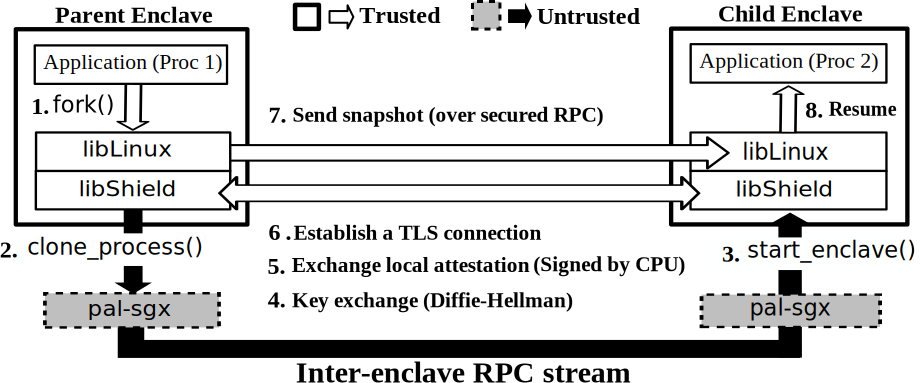
\includegraphics[width=5in]{graphene-sgx/figures/fork.pdf}
\footnotesize
\caption[Process creation in \sysname{}]
{Process creation in \sysname{}.
Numbers show the order of operations.
When a process forks, \sysname{} calls {\tt execve} system call
on the untrusted host,
to create a clean enclave with the same \libos{} image.
Then the two enclaves build up the mutual trust by
exchanging a session key, verifying attestation of each other,
and migrating the process snapshot from the parent.}
\label{fig:gsgx:fork}
\end{figure}

To secure process creation across enclaves,
\sysname{} is capable of building up the trust to newly launched enclaves,
through cooperation with an untrusted host.
Once a clean and trusted new enclave is launched,
The parent process will send a snapshot to the new one,
to create a clone of itself.
Snapshotting and migrating process states
is a feature robustly implemented and heavily used in \graphene{} \libos{},
of which we simply inherit the design.

When a process in \sysname{} forks,
because the parent and the child will be running the same binary,
both enclaves can simply be expected to have the same measurement.
To build up the trust, the two processes will open an encrypted channel
using a session key,
and exchange attestation generated by the processor.
Once both sides have confirmed the integrity of the other,
the parent process is safe to send its snapshot, encrypted, to the child
through the said channel.
The child process will restore the snapshot in its own enclave,
making it a clone of its parent.
The design of process creation in \sysname{} is shown as Figure~\ref{fig:fork}.

Forking in \sysname{} mainly defends against 3 types of attacks
from the untrusted host:

\begin{compactenum}

\item The host pretends to be the child enclave, to expose the process snapshot
sent from the parent.

\item The host pretends to be the parent enclave, to compromise the
child process using a malicious process snapshot.

\item The untrusted host becomes a man-in-the-middle, which bounces
encrypted messages between the child and parent enclaves, with session keys
negotiated with both sides.

\end{compactenum}

As described earlier, attacks 1 and 2 are prevented by mutual attestation
between the parent and the child,
and encrypting the channel for sending the snapshot.
The attestation signed by the processor proves that both entities communicating
are valid \sysname{} enclaves,
and encrypting the channel prevents the snapshot being eavesdropped or
counterfeited by the host.

To defend against attack 3 (the man-in-the-middle attack), we take advantage of
a user-customized 512-bit field
in the attestation structure generated and signed by \sgx{}.
This field is filled with a SHA-256 hash value of the agreed session key,
and the current enclave ID,
to prove that the attested enclave is the one who agrees on the key.

Once a parent enclave forks a child, by default the child must be trusted
to maintain its own security,
because the migrated snapshot discloses all information in the parent.
Unless the binary run in the parent enclave ensures
that no secrets is stored in the enclave memory at the time of snapshotting,
the parent enclave cannot simply drop the trust against the child.
For example, a pre-forked Apache web server may want to keep each worker
that responds to HTTP requests isolated,
to avoid being compromised by one attacked worker.
\graphene{} \libos{} provides an API for applications like Apache to explicitly
specify isolation to untrusted child processes.
\sysname{} inherits the ability of dynamic process isolation,
but developers are responsible for keeping confidential information
from the untrusted children.

\paragraph{Implementing {\tt execve}.}
Unlike {\tt fork}, {\tt execve} is used to
start processes with specified binaries, often different from the callers'.
When a thread in the process, either single-threaded or multi-threaded,
calls {\tt execve} in \sysname{},
\libos{} will migrate the calling thread to a new process,
with clean process states except opened files cloned from the parent.

The main challenge for implementing {\tt execve} is to
identify trusted binaries that can be loaded into new enclaves as child processes.
Consider the case where the parent process and its child shares
a multi-process abstraction (e.g., message queue).
Even if only the parent side is provisioned by the client, the child side
can still potentially compromise the secrets,
by exploiting vulnerabilities in the shared abstraction.
The trust between the parent and the child must be mutual,
unless the two enclaves are strictly isolated.

To identify binaries that can be trusted (either as parents or children)
during process creation,
\sysname{} requires each binary ported for an application,
to be shipped with a list of binaries that can be {\tt execve}'d,
and those that can be callers of {\tt execve} to the said binary.
Each binary in the list is identified by its measurement, which is mutually attested
between the parent and the child during process creation.
This list must be signed by a private key provided by the client,
while the public key must be included in the enclave measurement of the binary.

\subsection{Securing Inter-Process Coordination}
\label{sec:graphene:multiproc:ipc}

After process creation, a multi-process application often cooperate
through shared abstractions between processes,
such as signals or message queues.
For \libos{}, OS states for these shared abstractions must be shared
though inter-process coordination, for mainly two purposes.
First, for each abstraction, \libos{} needs to maintain the state
in one of its instances.
Second, \libos{} must maintain the namespace states to identify and locate the
abstraction states.

\graphene{} implements a wide range of multi-process abstractions and namespaces,
by passing messages over RPC streams among processes.
Such a design is perfect for porting multi-process applications to enclaves.
The benefit of sharing abstraction by RPC coordination are that
the enclaves will not have to share any memory to
coordinate abstraction states,
and the RPC streams can be secured by the enclaves instead of the host.

In \graphene{}, security isolation among multi-process abstractions,
regardless of their semantics,
are enforced by isolating the RPC streams used for coordination.
Unfortunately, \sysname{} cannot trust the host to faithfully isolate
the RPC streams.
Each enclave launched for an application must secure inter-process coordination
spontaneously, by only communicating to enclaves that it has attested
and exchanged secret keys with.
Because inter-process coordination is completely transparent
to the applications,
all information sent over RPC streams must be encrypted,
because \libos{} cannot determine whether the information may contain any secret.






%\section{Minimizing the TCB with the Non-Partitioned Model}

%\subsection{Reducing the TCB in \libos{}}
%\subsection{Partitioning the TCB in Multi-Process Applications}



\section{Implementation Details in \graphene{}}
\label{sec:graphene:impl}

\paragraph{Linux \pal{}.}
The majority of \pal{} calls are simple wrappers for similar Linux system calls, 
adding less than 100 LoC on average for translation between \pal{} and Linux abstractions.
The largest \pal{} calls are for exception handling, synchronization, and picoprocess
creation, which require multiple system calls and range from 500--800 LoC each.
Creating a new picoprocesses internally requires a {\tt vfork} and {\tt exec} of a clean 
application instance, and would be more efficiently implemented in the kernel.
Finally, the other major \pal{} components are an ELF loader (2 kLoC), headers (800 LoC),
and internal support code (2.3 kLoC).

\paragraph{Alternative \pal{} Ports.}
We prove the platform independence of \graphene{}
by porting \pal{} to \emph{FreeBSD}, \emph{OSX} and \emph{Windows}.
With the alternative host \pal{}, unmodified Linux binaries,
along with {\tt glibc} and {libLinux},
can be transparently run on the host.
For FreeBSD,
only 1.2 kLoC of the host \pal{} code need to be rewritten,
which are significantly less than FreeBSD Linux compatibility module (10.8 kLoC).
\pal{} components including ELF loader and internal support code can be shared by any \pal{} ports.

%\fix{We leave host \pal{} ports to non-unix OSes like Windows as future work,
%but previous works~\cite{porter11drawbridge,baumann13bascule} have already shown it feasible.}

\begin{table}[t!b!]
\footnotesize
\centering
\begin{tabular}{|l|rr|}
\hline
{\bf Component} & {\bf Lines} & ({\bf \% Changed})\\
\hline
GNU Library C ({\tt libc}, {\tt ld}, {\tt libdl}, {\tt libpthread}) & \libclines{} & $0.07\%$ \\
\hline
Linux Library OS ({\tt libLinux}) & 31,112 & \\
Linux host \pal{} & 11,644 & \\
Extra code for Linux \sgx{} host \pal{} & 9.354 & \\
% updated by Chia-Che on Oct. 10, 2013
\hline
%Storage Server & \fixmedp{XX} & \\
Reference monitor bootstrapper & \reflines{} & \\
Linux kernel reference monitor module ({\tt /dev/graphene}) & \sandboxmodlines{} & \\
Linux kernel IPC module ({\tt /dev/gipc}) & \gipclines{} & \\
\hline
\end{tabular}
\caption[Lines of code written or changed in \graphene{}]
{Lines of code written or changed to produce \graphene{}.  Applications and other libraries are unchanged.}
\label{tab:graphene:loc}
\end{table}


%% * most calls are a wrapper, \fixmedp{XX} LoC on average.
%% * Exception handling, sync, and process creation were harder (500-800 LoC each).  Process creation requires a clean instance (vfork+exec), would be simpler to implement in kernel.
%% * Other major components: ELF loader (2kLoC), headers(800 LoC), internal support code (2300 LoC)


%\fixmedp{Chia-Che, update LoC table}

\paragraph{Implementing Linux Personality.} 
%\fixmedp{Revisit the logical flow of these paragraphs}
The \graphene{} {\tt libLinux.so} implements a subset 
of the Linux system call API (currently \graphenesyscalls{} calls)
using only the \pal{} ABI to interact with the host.
We note that Linux exports a very long tail of infrequently used calls.
%applications.
A rough analysis of this tail indicates roughly 100 additional calls that can be implemented
with the existing \pal{} ABI and coordination framework, less than 10 administrative calls that will not make sense to expose to 
an application, such as loading a kernel module or rebooting the system, and roughly 54 that will require 
\pal{} extensions to meaningfully implement, such as controlling scheduling,
NUMA placement, I/O privilege, and shared memory.
In the last category of system calls, the degree to which actual host details should be exported versus emulated is debatable.

%We believe represent the most commonly used system calls.
%When an application requests a call or argument that {\tt libLinux.so} does not implement,
%the picoprocess exits with a distinct error message. 
Each time we have tested \graphene{} with a new application, the number of extra system calls
required has dropped---most recently we only added 4 calls
(namely, epoll\_create, epoll\_wait, semget and semop)
to support the Apache web server.
Thus, we believe \graphene{} implements a representative sample of Linux calls.

%such as {\tt sched\_setparam}, which manipulates scheduler-specific
%parameters or 
%{\tt uselib}, which has been abandoned 
%in {\tt glibc} version 2 in favor of a user-space dynamic linker.
%We do not plan to implement administrative interfaces, such as {\tt reboot}.
%The growth in the set of supported system calls has been driven by 
%the requirements of new applications we use to exercise \graphene{}, and has been 
%slowing considerably over time.

%directly to guests, and thus will not implement them in {\tt libLinux.so}.

% dp: :(
\begin{comment}
Most {\tt libLinux.so} code reimplements
Linux kernel functionality.  We found it expedient to 
read the Linux source in order to understand its behavior and then reimplement 
that behavior on the \pal{} ABI in most cases.
In some cases, such as the file caching code,
%directory entry (dentry) cache, 
we refactored code directly from the Linux kernel.
%% In these cases, we simplified data structures to only include data
%% we needed for a single application, and to hook in with other 
%% {\tt libLinux} subsystems.
%% An interesting direction for future work would identify techniques
%% to automatically import larger swaths of Linux kernel code, facilitating
%% adoption of new features and bugfixes.
\end{comment}

In order to use {\tt libLinux.so}, we modified \libclines{} lines of {\tt glibc} to replace 
system instructions with function calls into {\tt lib\-Linux.so},
and to cooperatively manage thread-local storage with {\tt libLinux.so} (Table~\ref{tab:graphene:loc}).

%All totaled, we only needed to modify \libclines{} lines of glibc source code to redirect all 
%system calls to {\tt libLinux} 

\begin{comment}
\vspace{5pt}
\noindent{\bf ABI Extensions.~}
\graphene{} extends the Drawbridge ABI with 9 additional \pal{} calls.
As discussed above, one creates a new sandbox, and 
5 additional calls were added for IPC.
We also add 3 calls to manage x86 segmentation registers
and exceptions (Bascule~\cite{baumann13bascule} adds
similar extensions).
\end{comment}

\paragraph{Synchronization.} Perhaps surprisingly, implementing Linux
synchronization appears substantially easier than Windows synchronization, 
as {\tt libLinux} did not require all of the various
synchronization ABIs provided by Drawbridge.
We believe the reason for this is that Linux has consolidated 
all user-level synchronization primitives to use futexes~\cite{franke02futex},
which are essentially kernel-level wait queues.
%In Windows parlance, this is simply an Event associated with a virtual address.
%Thus, our effort implementing synchronization was relatively straightforward.

%\subsection{Linux Host \pal{}}
\label{sec:linux:pal}

\begin{comment}
The Platform Adaptation Layer (\pal{}) exports a generic host kernel interface to the guest, summarized in Table~\ref{tab:abi}.
Our Linux host \pal{} consists of a user library and a small Linux kernel module.
Our \pal{} library is implemented using  \nativecalls{} native Linux system calls.
%The specific division of labor between the host kernel and user library
%could be different in another implementation.
%We currently implement only a Linux host \pal{}.  
If a different host kernel implements the same \pal{} ABI,
{\tt libLinux.so} and all binaries
should execute without modification.


%How we connect the shim to the \pal{}?  Expedient to hack the loader to add it to the link tables.  Describe.  
%-Dynamically linked, included in loader (ld.so can't mmap the \pal{}; conceptually should be mapped by the OS)
%-imported by libc
%-- Does a new binary type require kernel mods?  If so, make claim about unmod host
%-- conceptual leakage by tightly coupling pal and loader; pal should be provided by the host OS
% validated that no other native system calls
%% were being issued by application directly to the host kernel with {\tt strace} 
%% and by disassembling application binaries.
%% In future work, we will replace the native Linux system call table 
%% with a restricted system call (or hyper call) table to host.
%potentially migrating much of the \pal{} implementation into the host kernel.

We selected the Drawbridge ABI~\cite{porter11drawbridge} as a starting point for the \sysname{} ABI,
because it strikes a good balance between host platform independence 
and avoiding duplicate functionality.
In porting Linux to the Drawbridge ABI, which was designed for a Windows library OS,
we strove to only add additional interfaces when otherwise unavoidable for
functionality or performance.
In some cases, revisiting the Drawbridge design choices 
could simplify {\tt libLinux},
but we wanted to understand how well the Drawbridge design generalizes to other guests, 
without undermining its simplicity.
\end{comment}

%We note that we reimplemented the Drawbridge ABI according to the published description and 
%expect that both systems two could be interoperable
%with a modest amount of reconciliation effort where the published specification is ambiguous;
%because Drawbridge is not publicly available, we cannot test interoperability of the library OSes.


\begin{comment}

\noindent \sysname{} requires  the following additional \pal{} calls:
\begin{compactenum}
%% dp: I think these are the key ones
%\item \fixmedp{What is missing here}
% What is: DkThreadSelf - is this necessary?  
% DkThreadPrivate
\item {\tt DkSetSegmentRegister} --- Set the optional segmentation
  register values ({\tt fs} and {\tt gs} on {\tt x86\_64}).  This functionality 
  is required
  for thread-local storage, which is initialized in user-space
  by the Linux loader.
  The Windows kernel initializes these registers before process execution begins, 
  obviating the need to initialize them from user-space.
  We further note that different OSes use these registers differently
  (e.g., 32-bit Windows uses {\tt gs} for TLS, whereas Linux and 64-bit Windows use {\tt fs} for TLS),
  therefore management of these registers should be in the domain of the guest.
\item {\tt DkSetExceptionHandler} --- Register a callback for a hardware exception, 
  such as a divide by zero error or segmentation fault.  This is roughly analogous 
  to a software emulated interrupt descriptor table (IDT).  
  %In future work,
  %we will adopt techniques proposed previously to send processor exceptions directly to the guest~\cite{belay12dune}.
\item {\tt DkExceptionReturn} --- Returns from an exception back to the host kernel.
   %% In our current design, the host kernel is responsible for returning control flow 
   %% back to the thread that was running when an exception occurs.
   %% Alternatively, the \sysname{} ABI could require exception delivery to include
   %% a register trapframe sufficient to resume execution directly in user space.
% Async upcall; return necessary?
%\fixmetsai{I am not sure how to put this, but the design of Return is to leave \pal{} independent from its host semantic
%%%    With the extra call, guests no long need to worry about the stack structure that
%%%    \pal{} created at exception handling. For example, \pal{} might put extra objects on stack, or use an
%%% alternative stack. These design will make the guest crash while trying to return.
\item {\tt DkCreatePhysicalMemoryChannel}, {\tt Dk\-Physical\-Memory\-Send}, and {\tt Dk\-Physical\-Memory\-Recv} --- These calls mark a set of pages in the sender's address space as copy-on-write (COW) 
  and then map the pages as COW in the receiver's address space.
  Although these calls are not strictly required, as
  data can be sent over a stream, we found the ability to exchange 
  large quantities of data efficiently to be an important 
  performance optimization for {\tt fork}  (\S\ref{sec:fork}).

\item {\tt DkHandleSend}, {\tt DkHandleRecv} --- Send a stream 
  handle out-of-band to another guest in the same sandbox.
  This is used to establish connections both for namespace
  coordination (\S\ref{sec:namespaces}) and 
  handle inheritance (\S\ref{sec:fork}).
  

%  This mechanism required extending the Linux kernel with a \gipclines{} line module,
%  discussed below.
%  This module does not require any kernel changes or recompilation.
  
\end{compactenum}
\fixmedp{isolate pal call?}

%%% Extra \pal{} calls we needed.  Describe issues. \fixmedp{Can I get a list?}
%%% -mutex (don)
%%% -cv (don)
%%% -IPC physical memory calls send/recv
%%% -set\_thread\_private - sets segmentation registers for TLS
%%% -synchronous event - sets hardware exception handlers + OS callbacks (seg fault, div zero, external kill, async io, interrupts, etc.) roughly analogous to idt
%%% -system initialize - get control block address for checkpointing/etc. - avoids assumptions about address space layout

\paragraph{Fast bulk data movement.} 
We extend the Linux host kernel with a
fast bulk IPC mechanism.  The bulk IPC mechanism does a 
copy-on-write (COW) data transfer between two guests.
A sender designates virtual pages to send to 
the receiver;
these pages are then placed in a first-in-first-out queue.
The receiver then requests these pages be mapped into its address space,
optionally providing a target virtual address (similar to {\tt mmap}).
The sent pages need not be virtually contiguous, 
allowing the guest to efficiently gather and send scattered pages.
%This is useful for implementing guest-managed page caches.

\sysname{} uses bulk IPC in conjunction with control
messages on a byte stream; 
the byte stream communicates the expected meaning and ordering 
of the corresponding bulk data transfer.
In the common case, these physical pages are quickly shared between
two processes, minimizing data copying
for user-level implementations of system calls like {\tt fork}.
%The CAS server commonly
%unmaps sent pages, which will reduce the page reference 
%count to one and eliminate the need to copy the page on a 
%on a write fault in the receiver.

Our bulk IPC module is \gipclines{} lines of code, 
runs on multiple versions of Linux (2.6 and 3 series kernels), and
does not require
Linux kernel changes or recompilation.
\end{comment}

%% dp: So sad, but something has to go
\begin{comment}
\paragraph{Efficient creation of clean processes.}
We implement a process creation ABI in the host 
that only creates 
clean child picoprocesses that do not inherit memory mappings
or open file handles from the parent, similar to booting another VM.
This design choice strengthens security isolation.

Linux does not provide a process creation mechanism other than {\tt fork()} (or variants, such as {\tt clone()}).
Thus, the \pal{} is must implement this abstraction on Linux processes.
A simple implementation of {\tt Dk\-Pro\-cess\-Create()} would {\tt fork} 
a new process,
clean the open file handles, and then {\tt exec} the new binary.
This simple implementation of process creation
wastes work implementing an ABI that will always {\tt exec()} a clean process.
%%% The {\tt fork-exec} approach bring unwanted overhead to {\tt fork} and {\tt execve}
%%% system call. Compare to the native system calls, reloading the whole \sysname{}
%%% system causes duplicated works such as parsing manifests and linking libraries.

The \pal{} optimizes process creation by forking 
a newly launched picoprocess after initializing all of the operating system state,
but before starting any application-specific work, such as calling the ELF loader.
Dune leverages a similar optimization to efficiently create
isolated threads in the Wedge case study~\cite{belay12dune}.
The checkpoint process is not visible to the application.
This checkpoint listens for a message from the \pal{} to 
fork itself in order to create a clean child.

Because new processes are created by forking the checkpoint process,
as a guest creates children, they are actually siblings
from the perspective of the host kernel.
The guest implements the abstraction of a Linux process tree inside the library OS.

This checkpointing strategy works well even if the application 
requests that the child load a different application
binary, because the checkpoint is taken before {\tt ld.so} links in the application.
In a simple microbenchmark,
this checkpointing strategy improved picoprocess creation time
 a factor of two.

%This approach is \fixmedp{XX\%} faster than simply {\tt exec}-ing 
%the \pal{} in the child to clean up parent state.

%%% This strategy of checkpointing the process manager allows \sysname{} to quickly 
%%% create clean child processes in user-space on an unmodified Linux kernel.  
%%% In a simple microbenchmark,
%%% this pre-forking strategy improved {\tt DkProcessCreate} time
%%% by a factor of two.


\end{comment}




\section{Implementation Details}

\paragraph{Linux Personality.}

\paragraph{Memory and Binary Loading.}

\paragraph{Exception handling.}

\paragraph{Securing RPC streams.}

\paragraph{Attestation.}

\paragraph{Framework Support.}


\declarecommand{\sysname}{\graphene{}}
\declarecommand{\pal}{PAL}
\declarecommand{\syscalls}{131}
\declarecommand{\palcalls}{43}
\declarecommand{\nativecalls}{50}
\declarecommand{\gipclines}{1,131}
\declarecommand{\sandboxmodlines}{888}
\declarecommand{\reflines}{3,568}
\declarecommand{\libclines}{606}
\declarecommand{\interfacenum}{41}
\declarecommand{\light}{lighttpd}
\declarecommand{\gcc}{gcc}
\declarecommand{\lmbench}{LMbench}
\declarecommand{\ab}{ApacheBench}
\declarecommand{\busy}{Bash}
\declarecommand{\skylake}{Skylake}

\chapter{Evaluation}
\label{chap:eval}
\section{Summary}



The Linux PAL successfully leverages a limited subset of Linux system calls,
to implement the whole PAL ABI for running a
full-featured \libos{}.
\Thehostabi{} separates the development of a host OS or hypervisor
from the complexity of emulating a sufficiently-compatible
Linux kernel.
The chapter shows that most calls in \thehostabi{}
can be directly translated to similar system calls on a Linux host kernel.
Only a few \hostapis{}, such as process creation and inter-thread synchronization, require additional attention for developing an efficient implementation strategy.



The Linux PAL also enforces robust security isolation
between mutually-untrusting applications,
by placing applications in separate, VM-like sandboxes.
The security isolation on a Linux host is based on system call restriction using a \seccomp{} filter, and a trusted reference monitor. % for checking resource access.
Security isolation at the host interface
restricts an untrusted application to explore vulnerable execution paths
inside a Linux kernel.
A \seccomp{} filter 
enforce a fixed, minimal system call profile, regardless of bloated dependency of an application.
The reference monitor follows
simple, white-listed manifest rules listing 
all the authorized files and network addresses of an application,
using well-known semantics
such as AppArmor~\cite{apparmor} or iptable-like firewall rules~\cite{iptablesman}.
The reference monitor can further enforce dynamic, process-specific isolation by splitting a sandbox
to run a child \picoproc{} under more restricted
resource permissions.
\graphene{} on a Linux host can serve as a sandbox framework
with a reduced attack surface
upon the host kernel.








\chapter{\java{} Applications on SGX}
\label{chap:civet}


\newcommand{\sysname}{Civet}
\newcommand{\jvm}{JVM}
\newcommand{\jvmname}{OpenJDK 7}
\newcommand{\staticphase}{design-time}
\newcommand{\statictool}{Shredder}
\newcommand{\dynamicphase}{execution-time}
%\newcommand{\dynamicframework}{Escalator}
\newcommand{\dynamicframework}{Connector}
\newcommand{\tcbsize}{trusted code size}


\makeatletter
\newcommand{\Capitalize}[1]{%
	\edef\@tempa{\expandafter\@gobble\string#1}%
	\edef\@tempb{\expandafter\@car\@tempa\@nil}%
	\edef\@tempa{\expandafter\@cdr\@tempa\@nil}%
	\uppercase\expandafter{\expandafter\def\expandafter\@tempb\expandafter{\@tempb}}%
	\@namedef{\@tempb\@tempa}{\expandafter\MakeUppercase\expandafter{#1}}}
\makeatother

\Capitalize{\dynamicphase}
\Capitalize{\staticphase}


\makeatletter
\def\input@path{{civet/}}
\makeatother
\graphicspath{{civet/figures/}}

\begin{abstract}

  Application partitioning is a technique to move sensitive data or code into
  a protected environment, such as an SGX enclave.
  Partitioning larger existing applications requires subtle reasoning that can be aided with static
  analysis and dynamic, language-level techniques.
  For instance, in-enclave code may include a library that memoizes results in the out-of-enclave heap.
  Using a managed, type-safe language like Java in SGX also brings the benefits of partitioning to a large body of 
  existing code. %, as well as help the developer with language-level analysis tools.
  Unfortunately, running Java partitions in SGX introduces a number of technical
  challenges, many of which arise from resource and system ABI constraints.
  To our knowledge, no prior work has even run a complete Java application in an enclave,
  much less partitioned a Java application to run a piece of application logic in the enclave.
%  That said, no amount of application-level analysis can protect against
%  a compromised OS, without 
  Thus, a number of technical challenges must be addressed to unlock
  the benefit to developers of combining managed languages with hardware such as SGX.


%% \fixmets{Streamlined the argument for combining Java and SGX. Check if this makes sense.}
%% %%There have been significant, but separated %often mutually exclusive,
%% There have been significant, but often mutually exclusive
%% advances in hardware and language-level tools for partitioning applications
%% into multiple security contexts or privilege levels.
%% %Developers who build security-sensitive applications
%% %often face the dilemma of choosing between
%% %managed language features and hardware protections with language restrictions.
%% Developers either 
%% use a hardware solution, such as \intel{} \sgx{},
%% to isolate a piece of consolidated code %small piece of native binary code
%% from an untrusted OS, %but the developer
%% %must reason carefully about potential information flows that could leak data from the enclave, as well as other vulnerabilities in the code.
%% %On the other hand, in
%% or choose to program in a managed type-safe language, such as Java, 
%% %the developer has 
%% which has a wealth of tools and properties for 
%% improving code security and application partitioning.
%% %from type-checking to 
%% %more advanced tools to secure control and information flows.
%% The use of hardware
%% and language-level tools for partitioning are often complementary by concept but incompatible in reality.
%% %mutually exclusive,
%% %due to the limitations in combining the technologies.
%% %This paper observes that these language and hardware security tools 
%% %should complement each other, but are often mutually exclusive.
%% For instance, no language-level analysis %of an application
%% can protect an application against a compromised OS.
%% However, it is fundamentally challenging to
%% factor the protection of \sgx{} into the analysis of a managed type-safe language like \java{}.
%Running a managed language in an enclave is difficult, and language tools
%currently do not factor the hardware capabilities of \sgx{} or similar hardware into their analyses.


%Similarly, the \sgx{} hardware imposes restrictions on loading \java{} classes 
%with \jvm{}s;
%the \java{} language also lacks sensible APIs for using \sgx{} hardware.
%to wrap the semantic of interfaces with the 

%but are not sufficient to defend against a compromised OS or hypervisor.
%but the developer must partition the application 
%and harden the code inside the enclave.
%Managed languages, such as \java{},
%offer a wealth of language-level support for 
%but are not sufficient to defend against a compromised OS or hypervisor.
%The two approaches are often mutually-exclusive:
%we are unaware of any prior work thas has run a \jvm{} inside of an enclave at all,
%For \sgx{} and \java{},
%there is no prior work that has run a \jvm{} inside an enclave,
%much less integrated enclaves into the language's analysis tools.
%\fixmedp{check my claim. Too strong, or justified?}
%\fixmets{Since we are generalizing, we should only claim this is the case for sgx vs. Java. BTW, I prefer showing more certainty when making claims.}


%Application developers can place a library and sensitive data
%in an \intel{} \sgx{} enclave,
%but only if the library is a native binary, generally written in C.
%but must relies on developers to design invulnerable code.

%more advanced tools for detecting information flows.

%These language-level tools can be invaluable in ensuring a correct application partitioning
%and overall application correctness.
%Unfortunately, the most security-sensitive developers must choose between
%hardware and language security tools.


%% Using \intel{} \sgx{} enclaves, applications can
%% protect their most critical components from untrusted system stacks.
%% Language support for \sgx{} enclaves is a missing feature of existing \java{} Virtual Machines.
%% Using a managed language like \java{}
%% provides an opportunity to improve the weakest link of the enclave security---
%% application vulnerabilities that lead to information leakage.
%% \java{} language has effective framework to trace information flows, and provides type safety
%% to prevent memory access vulnerabilities in the enclave.
%% In addition, modularization in \java{} classes allows automatically partitioning
%% an application into enclave components,
%% minimizing the classes included in the enclave's trusted computing base.

This paper presents {\em \sysname{}},
a system that integrates \java{} language tools for partitioning applications
with run-time support for isolated execution in \sgx{} enclaves.
%\fixmedp{Any reason we can't do more than one partition in the enclave?}
%\fixmets{For an application, there is only one partition: the secure-sensitive part. We can create more than one instances in an enclave.}
%and which can execute a portion of the \java{} application in 
%a \java{} utility, runtime framework and API,
%that helps developers design isolated application components,
%and minimizes the attack vectors.
\sysname{} includes both \staticphase{} and \dynamicphase{} components.
The \staticphase{} tool, {\em \statictool{}}, uses code reachability analysis
to determine the minimal required \java{} classes for the isolated execution,
and helps the developer understand the complete partition interface. % between the application partitions.
%\sysname{} helps the developers generate an enclave image
%with minimal required \java{} classes for the protected code, reducing the TCB. %required for isolated execution.
%%\sysname{} includes language-level information flow control at the 
%%enclave border, protecting against unexpected exfiltration of secret
%%data due to application vulnerabilities.
The \dynamicphase{} framework, {\em \dynamicframework{}}, then launches the isolated execution of the enclave image
(a signed JAR archive) in an enclave when the untrusted part calls the interface.
Throughout the execution, \sysname{} enforces end-to-end isolation
on any object instantiated inside the enclave,
and leverages language-level information flow control to determine whether an object contains no sensitive information before the object is released from the enclave.
%to protect against unexpected ex-filtration of secret
%data. % due to application vulnerabilities.
%\fixmebj{How about this?}
%\fixmedp{Is this best-effort?  Only for explicit flows?  The 
%preceding sentence should be crisper}
%identifies information flow at the enclave border,
%preventing enclave secrets
%from being leaked due to any vulnerabilities.
%with minimal classes needed for the isolated computation,
%and narrowest interface for interaction.
%Second, the framework effectively prevents information leakage
%by forbidding any objects tainted by information flow to leave the enclave.
%In \sysname{},
%trusted servers may provision secure objects and classes,
%preserving security policy information. \fixmedp{Don't understand the previous sentence}
%\fixmedp{Do we want to say anything about contributing techniques to get good performance?}
%To secure \java{} applications, 
%With both the \staticphase{} and \dynamicphase{} language support,
\sysname{} also creates language-level abstractions of and extensions \sgx{},
such as attestation and provisioning, simplifying cumbersome aspects of this hardware
for developers.
%extends the security properties (e.g., data confidentiality) and features (e.g., attestation and provisioning)
%of \sgx{}, %hardware protection to cover \java{} classes dynamically loaded by the \jvm{},
%and encapsulates cumbersome aspects of interfacing with the hardware architecture
%keeps the work of bootstrapping and interfacing with 
%from application developers.
%As a proof-of-concept of using advanced language-level tools,
%we use \sysname{} %strengthens hardware protection
%to identify and remove 
%by filtering 
%implicit information flows that would leak secrets from an enclave
 % that leaks secrets
%in our test applications.
%\fixmedp{all of them?  Or just one?}\fixmets{I think this technique applies to all test cases.} % error-prone applications. 
%Finally, the API allows components in enclaves to be seamlessly provisioned with
%secure objects or classes by trusted servers,
%and to preserve their security policy information.
%with security guarantees extended from their sources.
%\sysname{} is evaluated with \jvmname{} on the latest 
%We evaluate \sysname{} % with several case studies 
%on the latest \intel{} Skylake processor.
%Evaluation shows good performance on
%Our overheads are low, 
%adding \fixmedp{xx}\% overhead on an isolated cryptographic library used in SSH client/server,
%and \fixmedp{xx}\% overhead on Hadoop jobs that run a secret, provisioned algorithm.
We demonstrate the usage of \sysname{} with two applications: a SSH server with an isolated cryptographic library to protect its host key,
and a Hadoop framework capable of securely executing jobs using any secret, provisioned algorithm.
%\sysname{} reduces the developer effort required to partition the application code,
%resulting in a smaller 
%and the result of integration is highly generalizable to other managed languages.
%~\fixmebj{Always replace TCB with code footprint size to indicate that we are only talking about size of code - not attack vectors.}
%\fixmets{find a better term for TCB size}
%~\fixmebj{Always replace managed languages with managed type-safe languages.}
%\fixmets{accurately separate managed language and type-safety: managed language causes the challenges, and type-safety improves the security properties; Java happens to be both.
%}
\end{abstract}

This chapter describes the formal definition of the \graphene{} host ABI.

\section{Basic Definitions}

The \graphene{} host ABI defines a set of {\em functions}, similar to the API of UNIX or POSIX.
The functions are directly called by the library OS, along with the arguments given either in the registers or on the stack.
A host-specific \graphene{} loader is responsible for resolving the linking, from the library OS to the host ABI.
%\papersection{Challenges for Partitioning with Enclaves}
\label{sec:background}
In this section, we will give a brief overview of \sgx{}, and discuss 
the key challenges developers face when trying to manually partition applications using a technology such as \sgx{}.
%discuss the programming models and threats to security of \sgx{} enclaves.

\papersubsection{Background on \intel{} \sgx{} Enclaves}

\intel{} \sgx{} ({\it Software Guard Extension})
is a set of new x86/x64 instructions
introduced in the \intel{} Skylake processor family.
Using \sgx{}, an 
application can designate part of its virtual memory as an {\em enclave}.
The CPU guarantees that the contents of the enclave never leave the CPU package unencrypted.
The CPU also measures the integrity of a binary loaded into the enclave, and offers remote attestation,
similar to a TPM\fixmedp{cite}.

%%% create a protected memory region, called an {\em enclave}, inside it's virtual memory,
%%% where it can load its security sensitive data with hardware-enforced isolation from the untrusted OS. 
%%% The processor with \sgx{}
%%% guarantees that any data loaded in enclave
%%% stays encrypted in the DRAM, by using a secret key deterministically derived from the application's cryptographic measurement and the CPU secret. 

\sgx{} is an appealing tool for protecting small amounts of highly-sensitive data or code, because it can defend 
against a malicious or compromsed OS, hypervisor, or even hardware peripheral.
For instance, \fixmedp{Foo} et al.~\fixmedp{cite that \sgx{} workshop paper} show how \sgx{} can be used
to build a trusted path from a video chat application to a GPU and network card, which maintains confidentiality and integrity of the
video stream, even if the OS is compromised.
Simlarly, because DRAM contents are encrypted, \sgx{} can resist cold-boot attacks~\cite{halderman09coldboot} or 
malicious peripheral devices~\cite{hudson15thunderstrike}.


%%% \sgx{} also proves the integrity of loaded binaries to remote trusted entities
%%% using mutual attestation based on a symmetric key generated from the measurements of communicating entities.
%%% \sgx{} usage model mostly involve the launched enclave mutually attesting the trusted host
%%% to obtain provisioning of security-sensitive information
%%% through a trusted channel. Such an execution model leverages resources such as CPU and DRAM from vulnerable untrusted \sgx{}-enabled hosts owned by cloud providers
%%% by extending the trust from
%%% the hosts owned and trusted by the clients or service providers.
%%% For instance, \sgx{} can isolate the decoder engine in an enclave
%%% after authenticating the customers to enforce Digital Right Management (DRM) even if the digital data is hosted on an untrusted cloud server.

%Use cases of \sgx{} mostly involve the launched enclave
%retrieving a cryptographically signed attestation from the processor,
%to exchange security critical information with remote servers through secured channels.
%The effect is equivalent to expanding the trusted space from remote servers
%to the local end, to harness local resources such as CPU and DRAM.

%One must note that \sgx{} only promises the integrity of application binaries
%initially loaded in enclaves.
%The gap between integrity of binaries and complete security has to be filled
%by ones who develop and approve the applications.
%More specifically, the clients are responsible of
%testing whether the applications contain any vulnerabilities
%that lead to information leak.
%To minimize the risk of leaving any flaws in the applications unintentionally,
%developers often tend to cut down the trusted computing base (TCB)
%of the applications. With smaller TCB, clients who launched the enclaves
%can more easily reason about the thoroughness of securing the execution.

%%% The key strength of \sgx{} enclaves over other software-based isolation framework such as
%%% {\em Flicker}, {\em Inktag} or {\em Virtual Ghost} is
%%% the ability to defend against attacks at the hardware level.
%%% These software-based solution often
%%% rely on a hypervisor below the OS to isolate the applications.
%%% If the hardware is attacked,
%%% the attackers may still bypass the software checkpoints,
%%% or directly steal confidential information from the DRAM.
%%% For \sgx{}, the only hardware included in the TCB is the CPU package,
%%% and in practice CPUs are believed to be hard to attack.
%%% Using techniques like cold-boot attacks~\cite{halderman09coldboot}
%%% to peek into DRAM content,
%%% or intruding the boot process using corrupted peripheral devices like Thuderstrike~\cite{hudson15thunderstrike}
%%% will affect any software-based isolation, but not \sgx{} enclaves.

\paragraph{Non-Partitioned Applications.}
One approach to using \sgx{} is to run an entire application in the enclave.
This is exemplified by Haven~\cite{baumann14haven}, which runs a \win{} application and all supporting libraries
on top of a {\em library OS}.  This approach is illustrated on the left side of Figure~\ref{fig:libosvssdk}.
The library OS approach does not require any application changes, but bloats the TCB \fixmedp{Rough number of how big Haven is}.
By pulling millions of lines of extraneous code into an enclave, there is a significantly increased risk 
of vulnerabilities that disclose
sensitive data, such as Heartbleed~\fixmedp{cite}.
The library OS approach is useful in its simplicity of deployment and can provide practical benefits, 
such as protecting an application from an untrusted cloud hypervisor.

\begin{figure}[t!]
\centering
\includegraphics[width=\linewidth]{figures/libosvssdk.pdf}
\footnotesize
\vspace{-0.2in}
\caption{
Comparison between the libOS-based model (e.g., Haven)
and the partitioned model for programing applications in enclaves.
Green (light) boxes are trusted components and red (dark) boxes are untrusted.
The libOS-based model yields a larger TCB in the enclave,
while the partitioned model requires developers to be responsible for determining the untrusted interface at the enclave boundary.
}
\label{fig:libosvssdk}
\end{figure}


This paper focuses on a second usage model for enclaves, where the application is partitioned into
untrusted and one or more trusted components (right side of Figure~\ref{fig:libosvssdk}).
Sensitive data and computation are placed inside of enclaves.  This approach requires the developer to
identify sensitive code and data; design and harden an interface between trusted and untrusted components; 
modify the application source; and reason about potential information flows at the enclave boundary.
This effort can be non-trivial and subtle, but for application developers motivated by interests such as 
regulatory compliance or competitive advantage in business, the additional effort can yield a much smaller trusted computing
base (TCB), and thus a reduced attack surface.
A key goal of \sysname{} is to minimize the developer's effort to partition an application---both in lines of 
code changed, and in leveraging language analysis to reason about narrow points in the application's data and control flow.


%To achieve smaller TCB, the software development kit of \sgx{}
%intends to encourage developers to partition the applications and
%keep only security sensitive components in the enclaves.
%Such an intention is exactly contradicted by the trust model of \haven{},
%which must trust the loaded application as a whole.
%Except for the cases in which the whole applications must be secured,
%\haven{} actually downgrades the trustworthiness of enclaves.
%Figure~\ref{fig:libosvssdk} shows the comparison of the two models.

%%% In prior works using \sgx{} enclaves to secure applications,
%%% developers choose between two different programing models: the {\em library-OS-based} and the {\em partitioned} model (as shown in Figure~\ref{fig:libosvssdk}).
%%% In the libOS-based model, developers run the whole standalone,
%%% legacy application inside the enclave, using library OS such as {\em Haven} or {\em Graphene libOS} to facilitate the rich OS features.
%%% The main benefit of using library OS is that developers only have to employ minimal efforts to port any existing application.
%%% Even when designing new applications, developers bear no responsibility
%%% of identifying and reasoning about
%%% the security sensitive part of the application.

%%% However, when using libOS-based model, a sophisticated legacy application
%%% will yield huge trusted computing base (TCB) in the enclave,
%%% aggravating the risk of leaking information through vulnerabilities inside the enclave.
%%% Known bugs such as {\em the heart-bleeding bug} has shown that
%%% running security sensitive code like an encryption engine, and management code such as heart-beating service in the same address space
%%% can cause vulnerabilities that compromise the security by leaking the encryption key.
%%% As a result, using a partitioned model, developers can isolate only the most security sensitive components in an enclave,
%%% and leave the remaining code outside to minimize the TCB.

%%% Developers have to define the {\em untrusted interface} 
%%% to allow parts of a partitioned applications to interact.
%%% The untrusted interface is used either by the the untrusted components
%%% to trigger execution of the isolated components,
%%% or by isolated components to use untrusted rich OS features, such as networking for provisioning and sending the execution output to the remote hosts.
%%% Unlike the libOS approach that has a fixed untrusted interface (for different applications) at their interaction boundary with the OS,
%%% the width of untrusted interface for a partitioned application is up to developers' design.
%%% The \intel{} SDK for \sgx{} supports a set of syntaxes to specify the type and direction of flow for parameters of the untrusted interface, and enforces primitive
%%% type-checking of incoming values on transition to enclave.

%%% The trade-off between the libOS-based and partition model is based 
%%% on ease of development, the width of untrusted interface,
%%% and size of TCB.
%%% The benefit of the libOS-based model is that developers can save the effort
%%% of determining what to execute in the enclave,
%%% and whether the execution is safe,
%%% because the whole application is wrapped in the enclave.
%%% However, the risk of having vulnerabilities in the applications
%%% is not reduced, but in fact amplified due to the addition of
%%% the library OS (e.g., the Haven binary yields around a few hundred MBs) to TCB.
%%% On the other hand, if the developers are willing to spend effort on carefully identifying the untrusted interface and re-designing their application around this interface, the partitioned model can improve security guarantees by minimizing the attack vectors.

%%% The goal of \sysname{} is to provide the benefits of both models.
%%% \sysname{} support a partitioned model
%%% for developers to isolate security-sensitive part of a \java{} application in enclave,
%%% and provide a language-based tool to automatically partition
%%% the minimal supporting classes to generate the enclave image.
%%% Even in the case where the isolated component need to frequently interact with the untrusted component or the OS,
%%% the language protection technique of information flow tracking
%%% guarantees that the secrets in the enclave are never leaked
%%% without the developers explicit consent. 

\paragraph{Side Channels and Denial-of-Service.}
In the current \sgx{} design, side channels are a signficant concern for either the library OS or partitioned model, and are out of the scope of this paper.
A controlled channel attack~\fixmedp{cite} can single step enclave execution by inducing page faults
in the enclave.  \sysname{} does not specifically defend against side channel attacks,
and we expect that any solution to this problem involves redesigning the division of labor in virtual
memory management for enclaves.

Similarly, there is no guarantee that a compromised application will ever enter
an enclave.  Denial-of-service attacks are out of scope for this paper.


\papersubsection{Challenges for Application Partitioning on \sgx{}}

\sgx{} provides useful building blocks for secure applications, but does not
absolve the programmer of any responsibility for reasoning about end-to-end security.
Bugs in the application or supporting libraries can still disclose sensitive data from an enclave,
and porting code into \sgx{} can be subtle.
This subsection outlines several pitfalls in partitioning an application for \sgx{}.

%%% \sgx{} enclaves provide strong isolation guarantee for applications,
%%% against the malicious or vulnerable application components, system stack,
%%% and hardware (except the CPU itself).
%%% However, the security guarantees of the \sgx{} enclave is dependent on whether the developers design perfect applications without exploitable vulnerabilities that may compromise the application's security.
%%% As the application developers are not perfect,
%%% even applications or components isolated in enclave can face threats to their security.
%%% As follows, we discuss a few potential threats
%%% to the enclave security,
%%% even under the assumption that the \sgx{} hardware is implemented as completely secure --- which can be another threat otherwise. 

%\fixmedp{I roughly want the rest of this section to have a problem, explanation, solution structure, with the overall theme being that this is subtle and we really need some analysis tools to get this right}

\paragraph{Writes outside of the enclave.}
\sgx{} allows code inside the enclave to read and write data structures 
outside of the enclave.  Thus, it is easy for a developer to inadvertently write
code that discloses a secret, say by using a library that memoizes intermediate results to the untrusted heap.
A fundamental requirement is that developers must be able to reason about (or assert)
what code can and can't access data {\em outside} of the enclave.
\fixmedp{Can we say anything about whether such tools exist before Civet?}

%\fixmedp{Do I recall correctly that you can easily write to data outside of the enclave?  If so, this seems like something easy to get wrong, especially 
%if a library memoizes intermediate results.  The developer needs to be able to tell 
%Unless I am full of shit, can we paragraph-ize this fixme?

\paragraph{Application vulnerabilities.} 
The major source of threats to enclave security is any internal vulnerabilities in the isolated components,
such as buffer overflows and other memory corruption attacks.
Moreover, although \sgx{} code integrity guarantees make enclaves resistant to code injection,
an attacker may still manipulate control flow using code-reuse attacks~\cite{code-reuse-attacks}.
Moreover, recent research ~\cite{hudata} show that even with perfect control flow integrity,
attackers can still manipulate the execution to leak the secrets through information flow.

Fundamentally, this argues for some combination of static analysis
and runtime monitoring of 
enclave code.  This is greatly simplified when the enclave code is written in higher-level languages
with properties 
%amenable to analysis.
%with type safety, memory safety, and other 
%that provide important 
%safety properties,
such as type safety or memory safety. %, thereby reducing the likelihood of these vulnerabilities.
Ideally, one would formally verify security properties of enclave code~\cite{moat}; this verification is significantly aided by using 
higher-level languages amenable to formal reasoning.
%Verification is significantly harder
%with C or x86 assembly.

%% \paragraph{Applications are not perfect} 
%% The \sgx{} hardware cannot prevent applications from copying secrets out of the enclave without limiting functionality.
%% The trusted isolated components can copy any sensitive data from the enclave to the unencrypted memory, and potentially leak the enclave secrets.
%% The primary risk in the isolated components
%% is often memory corruption vulnerabilities, such as buffer overflow,
%% %Because in enclave applications can access any part of out-of-enclave memory unrestrictedly,
%% prevalent in applications that are not implemented in type-safe languages.

%% The best known technique to prevent vulnerabilities is to model the applications and verify them using {\em formal verification}.
%% While Sinha et.al.,~\cite{moat} use formal verification to prove confidentiality of enclave programs, it is impractical to accurately model complex sophisticated applications.
%% As a result, in addition to formal verification, maintaining smallest TCB
%% in the isolated components is the most practical approach 
%% to ensure enclave security,
%% and is the main reason to choose partitioned programming model over
%% libOS-based model.


\begin{figure}[t!]
\centering
\includegraphics[width=\linewidth]{figures/partition.pdf}
\footnotesize
\vspace{-0.3in}
\caption{
Partitioning --- either manually or by automated tool ---
often causes wider boundary of partition than the actual security sensitivity boundary
due to (a) design granularity : {\tt secHelper} contains a {\tt send()} method that is not partitioned from the rest of the class by design.
The reasons of having the gap vary, for instance, 
that is less security sensitive, but due to the granularity it is not partitioned from the rest of the class or (b) better performance :  the less security sensitive {\tt logger} class is kept in the privileged level to service frequent method calls.
}
\label{fig:partition}
\end{figure}

%However, even if developers partition the applications and run only
%security sensitive components in the enclave,
%the developers may still leave some code irrelevant to
%enclave secrets inside the enclave.
%The reasons of having more-than-minimal TCB in enclaves
%are often that developers have to partition code in the granularity of source files or functions,
%or developers have to import more code to limit the width of interface and
%the frequency of interaction with the untrusted code.

\paragraph{Identifying ``pinch points''.}
Reasoning about where in a program to draw the line between 
trusted and untrusted code is subtle.
On one hand, the developer has an incentive to minimize the size of the 
API between the enclave and untrusted code, as well as an incentive to
minimize the total code in the enclave.  These goals can sometimes be at odds.
Each entry and exit to an enclave has a cost roughly comparable to a
process context switch\fixmedp{right?}; an easy way to reduce enclave entries and exits is to simply 
pull more code into the enclave, which increases the size of the TCB.

\fixmedp{I'm not sure how to explain Figure~\ref{fig:partition}, but it needs an explanation.}

Fundamentally, the art of paritioning an application is to find a ``pinch point'' or
``narrow waist'' in the application, where there is a natural point to insert an API and 
security checks.  This is indeed as much art as science, often done manually by experts\fixmedp{any more supporting evidence or cites?}.
It is unlikely that the average developer will successfully navigate this design process without analysis tools, such as \fixmedp{examples?},
to help identify these natural division points.


%% Experts can use a manual partitioning technique to achieve smallest TCB for the isolated components compared to automated tools.
%% However, the manual partitioning costs a lot of effort,
%% and rare expertise, lack of which can cause larger TCB.

%% Neither manual nor automated partitioning is perfect:
%% the resulted boundary of partitioning often has a gap from the actual boundary of security sensitivity (as shown in figure~\ref{fig:partition}),
%% leaving more code in the privileged level
%% than what's actually needed.
%% Having the gap between the ideal and resulted boundary
%% is mostly inevitable, due to multiple reasons.
%% One common reason is the granularity of partitioning,
%% which can vary from a binary file, a component, a source file,
%% a class, a method (a function) to a line of code.
%% Another reason is that a component or a method may be too frequently called
%% by the security sensitive code,
%% laying the boundary between the component or method from the security sensitive side may bring too much overhead or risk,
%% because the execution crosses the boundary too often.
%% Therefore, developers often will balance among the effort of partitioning,
%% risk or cost of communicating between different partitions,
%% and minimizing the TCB in the security sensitive parts.

\fixmedp{Maybe move the commented paragraph below down into the design section?  I'd like to downplay the plugs for our work here, and instead fulfill these promises later}
%% \sysname{} automates partitioning of applications,
%% based on the boundary at the classes which the developers marked
%% as the interfaces of the enclave.
%% Only the classes that are depended by the marked classes
%% will be included in the enclaves,
%% to minimize the TCB.
%% Although not all classes pulled into the enclaves
%% are necessarily security sensitive,
%% the enclaves are protected from the potential vulnerabilities in those classes,
%% by the security guarantees of \java{} language,
%% and the information flow tracking in \sysname{}.

%Another threat to \sgx{} is the vulnerability of the 
%security sensitive code running in the Enclave. The 
%main guarantee of \sgx{} to isolate the secure data 
%from other components and privileged OS is undermined 
%if the Enclave code can be tricked to leak the 
%security sensitive data to the attacker. Executing 
%buggy code in \sgx{} enclave can inadvertently leak 
%information if the attacker can exploit memory-safety 
%vulnerabilities like buffer overflow and dangling 
%pointers.  

% Cumbersome and approximation to partition code
%The developers have to manually partition their code 
%into security sensitive and insensitive part. If this 
%partitioning is done by a novice developer, some of 
%the security insensitive parts of the application can 
%end up in the security sensitive part, increasing the 
%Trusted Computing Base(TCB). Moreover, the 
%partitioning of code is not straightforward, which 
%can also contribute to a less stricter TCB. The bigger the TCB, the more %vulnerable is the Enclave code to attacks.

% Buggy Code leads to inadvertant information leakage


% \sgx{} code only Integrity protected not confidential
%Moreover, \sgx{} only protects the integrity of the enclave code. The security critical part of the application is stored in plaintext while the secret data is provisioned securely after attestation. However, \sgx{} does not protect the confidentiality of enclave application code which may be executing a secret algorithm. \fixmebj{Talk more about the problem motivating security tag preservation.}
%\sgx{} can natively guarantee either code integrity or
%code confidentiality (as part of the enclave data), but not both.
%If application code is included in the enclave measurement and
%verified by the hardware,
%the code must stay in plaintext as part of the enclave image.
%If any code is stored or provisioned in encrypted forms,
%the application or infrastructure in enclave must dynamically load
%the code after decryption.
%Supporting dynamic loading makes enclaves open to code injection
%if the applications have exploitable vulnerabilities.

\paragraph{Code Integrity {\em and} Confidentiality.} 
The hardware-level \sgx{} code integrity mechanism is based on a cryptographic
signature of a static binary in plaintext.
If any application dynamically loads any code after the enclave's initial measurement,
the initial application must be trusted to attest the loaded code.
The subtle tension is that there is no way to protect the confidentiality of
a secret algorithm, except by dynamically loading an encrypted binary.
Dynamically loading code increases the risk of code injection attacks and other control flow compromises.

Any application partitioning solution that protects sensitive algorithms
must have a robust dynamic loader that can measure encrypted libraries or classes.
\sysname{} includes a loader that can measure encrypted class files,
provisioned from a trusted host.

%% \sgx{} enclaves require code integrity in the isolated applications.
%% If the code integrity is not maintained, adversaries can corrupt the enclave code to
%% force the applications to leak the information provisioned from the remote,
%% trusted hosts.
%% \sgx{} hardware only guarantees
%% the integrity of the code initially loaded into the enclaves.
%% However, if an application choose to dynamically
%% load any code after the enclave starts,
%% the application is responsible for the integrity of the code loaded.
%% The fact that dynamic loading of applications, libraries or components
%% is a feature that can potentially make enclaves vulnerable and open to code injection,
%% raises concerns against supporting managed languages in the enclaves.

%% On the other hand, code confidentiality can be a desirable feature,
%% for application developers who prefer keeping the secret sauce of their algorithms concealed.
%% To enable the feature of code confidentiality in enclaves, the protected code must be dynamically loaded into the enclave,
%% because the \sgx{} hardware only accept
%% the initial loaded code to be in plaintext.
%% \sysname{} provides both code integrity and confidentiality by verifying
%% every classes dynamically loaded into the enclaves,
%% and allows loading classes provisioned from trusted hosts.


%% In general \sgx{} enclaves are prone to having side channels, such as timing channels. Because \sgx{} relies on the untrusted OS for paging,
%% an enclave will always leak page fault addresses, except the lower 12 bits (offsets in pages).
%% Such a leakage gives the untrusted OS to amplify the side channels,
%% by forcing page faults on every instruction or memory access.
%% This so-called {\em Controlled Channel Attack} is common to all applications who use \sgx{} protection, regardless of the programming models.
%% \sysname{} does not specifically defend against side channel attacks.

%% \paragraph{Denial-Of-Service Attacks}
%% \sgx{} is not designed to be safe against denial-of-service attacks.
%% Because the untrusted OS still controls the host resources,
%% there are countless ways to prevent an enclave from making progress.
%% For example, the OS can simply starve the enclaves by
%% never scheduling CPU, memory or other resources to the enclaves.
%% \sysname{} does not specifically defend against denial-of-service attacks.

\paragraph{Discussion.}  This
section has outlined several pitfalls for developers of partitioned applications.
These common pitfalls render the hardware protections of \sgx{} useless.
Language-level analysis can automate error-prone reasoning in the best case, or, in the worst case, 
can at least offer invaluable guidance to the developer.  For \sgx{}-style
hardware to be useful to a wide array of developers, developers need language-level
tools that can also factor in hardware-level protection mechanisms.



%- Motivate the problem.
%- List all attack vectors
%- How can JAVA help?




















































































\input{background2}
%\section{Threat Model}
\label{sec:threat}

In this section, we discuss the threat model of \sysname{},
including the adversaries,
and the components that must be trusted.

\paragraph{Adversaries}
We assume the same adversaries as other \sgx{} enclaves.
Any part of the system stacks, including the OSes,
device drivers, hypervisors, and even hardware,
such DRAM, GPU, buses, and peripheral devices, can be malicious
and attempt to attack the enclaves.
%The only trusted component is the CPU package, including L2 and L3 caches.
The attackers can perform any form of
online and offline attacks.
We also assume the attackers own all information
about \sgx{} hardware implementation, as well as every part of our solution.

We focus on the adversaries that target on
exploiting vulnerabilities in the isolated applications.
The attackers can manipulate any input to the application interfaces,
or the untrusted interfaces of the enclaves.
%Attackers may apply any techniques that compromise a regular privileged applications to compromise enclaves.
The vulnerabilities that attackers can exploit may not only fall in applications, but also in the infrastructures,
such as the libOS, the \java{} VM, JNIs and low-level interface to architecture.

%The only adversaries that are not addressed in \sysname{} are
%attackers exploiting {\em side channels} and
%{\em denial-of-service attacks}.
%Side channels, or even controlled channels, is a known problem of \sgx{} enclave
%and we expect to solve the problem in the future with
%stronger architectural support.
%Denial-of-service attacks are often considered benign for enclaves,
%because it only affect the ability of an untrusted host to legally access
%critical resources.

\paragraph{Trusted Components}
We trust any components loaded inside an enclave,
including the infrastructure (details discussed in Section~\ref{sec:implementation}), %(low-level interface, the libOS, \jvmname{}),
all supporting classes and their JNI,
and other resources or classes provisioned from remote hosts.
%All trusted components must be verified by either \sgx{} hardware or the infrastructure against their cryptographical measurements or checksums.
The implementation of \sgx{} hardware is also trusted to be invulnerable,
and use adversary-resistant key generators that cannot be compromised
by online or offline techniques.
We also assume \intel{} CPUs are resistant to direct, physical attack to the CPU packages, either to modify or peek into the chips.

\fixmets{Now JIT'ed code is not giving me error, but in case it fails later, we have to flip this discussion.}
We support running \java{} application both with and without JIT optimization.
Running \java{} application with JIT optimization
improve the performance of execution,
but can cause massive increase of the TCB of enclaves.
In case that JIT optimization is enabled in the enclaves,
the JIT compilers (\java{} VMs often have multiple JIT compilers, e.g., \jvmname{} has two) must be trusted by the users,
to always generate correct and invulnerable binary code.


%Note that in \sysname{} we disable JIT compiler that used to improve \java{} execution performance.
%The choice of disabling runtime compilation is due to the concerns that
%JIT compiler may largely extend the TCB because it must be trusted,
%and any bugs in different versions of compilers
%may causes code behaviors than what developers have tested and expect.
%Another practical reason is concerning the complexity and
%resources required for running a \java{} compiler with library OS in an %enclave.
%However, we consider these limitations to be not fundamental to the approach, and we keep compiler support in \sysname{} as a future work.



%In term of architecture, we trust the implementation of \sgx{} hardware,
%to maintain invulnerable implementation of \sgx{} instructions,
%and using adversary-resistant key generators that cannot be compromised
%by attacker using online or offline techniques.
%The CPU must keep enclave contents encrypted in DRAM and low-level caches that are shared by multiple cores.
%We also assume \intel{} CPUs are resistant to direct, physical attack to the CPU packages, either to modify or peek into the packages.

%\sysname{} protects confidentiality and integrity of provisioned security critical data in the trusted part of an application written in a high level managed language like JAVA.
% from the privileged operating system and the untrusted part of the same application. 
%\sysname{} assumes that the \sgx{} instructions are implemented correctly in the processor, and the SDK do not contain exploitable bugs to leak information. In addition, \sysname{} trusts the Graphene LibOS and the JVM running in the enclave with the trusted part of the application to not leak information. Thus, the security of the provisioned data is limited by the correctness of the processor, \sgx{}, Graphene LibOS, and JVM. \sysname{} also trusts the trusted part of the application to not leak information explicitly. \sysname{} prevents the trusted part of an application from implicitly leaking information.

%Threats that we do not cover
%\sysname{} inherits the threat model of \sgx{}~\cite{sgx}.
%The adversary controls the cloud provider's complete stack, OS, hypervisor, BIOS, system management mode, platform firmware, and device firmware. The adversary can also probe the memory and manipulate the I/O, but cannot read secret present in the processor.
%\sysname{} do not defend against attack vectors such as side-channel, covert-channel and control-channel~\cite{control-channel}. Denial of Service (DOS) attack is not part of \sysname's threat model. Even if the OS never schedules the enclave program or the untrusted part of the application is manipulated to never enter the enclave, no provisioned secret is leaked outside the enclave.


\papersection{Overview of the \sysname{} System}
\label{sec:overview}

This section provides an overview of \sysname{},
a system that assists developers in partitioning \java{} applications,
by combining \sgx{} hardware protection and \java{} analysis tools.
%with hardened security from both \sgx{}'s security guarantees and 
%\java{}'s safety features.
%% dep
%We will also discuss the threat model assumed in the design of \sysname{}.

\begin{comment}

%\begin{figure}[t!]
%	\centering
%	\includegraphics[width=\linewidth]{figures/alternatives.pdf}
%	\footnotesize
%	\caption{Alternative approaches to access \sgx{} hardware protection from \java{} applications.
%		The {\em libOS-based} approach runs the whole \java{} applications in the enclaves. 
%		The {\em JNI-based} approach uses JNI to run the security sensitive operations inside the enclaves.
%		The {\em \jvm{}-based} approach requires the \jvm{} to provide APIs to support common use cases of the enclaves.
%		Green (light) boxes are trusted components and red (dark) boxes are untrusted.
%	}
%	\label{fig:alternatives}
%\end{figure}

There are multiple approaches to access \sgx{} hardware from \java{} applications as illustrated in Figure~\ref{fig:alternatives}. Firstly, the whole \java{} application can run with the \jvm{} inside the enclaves,
using a \sgx{} like Haven~\cite{baumann14haven}({\em libOS-based}).
Secondly, the untrusted components of \java{} application
can run with the \jvm{} outside the enclaves, and a JNI wrapper can communicate
with the trusted component written in native language running inside the enclave like ~\cite{vc3}({\em JNI-based}). 
However,the JNI-based approach requires developers to have the knowledge of
enclave implementation, and loses the language protection of \java{} inside the enclaves.
A more plausible approach is to provide enclave-backed APIs
from the \jvm{},
to support common use cases ({\em \jvm{}-based})), such as a secure key-value store~\cite{vc3}.
Although the \jvm{}-based approach can save the application developers' effort
of implementing isolated components,
the use cases is limited to the pre-defined operations provided by the \jvm{} or the companion frameworks.
Because the backend implementation (isolated components and untrusted interfaces) in the \jvm{}-based approach is the same as the JNI-based approach,
the same language restriction also applies here. 

\end{comment}

\papersubsection{Design and Features}

\sysname{} consists of a \staticphase{} tool (\statictool{}) and a \dynamicphase{} framework (\dynamicframework{}):
%to help 
%developers to partition \java{} applications.

\paragraph{Partitioning \java{} applications into enclaves (\statictool{})}
To cleanly partition \java{} applications into
 trusted and untrusted components,
 \sysname{} provides a \staticphase{} tool called \statictool{}
%\fixmedp{I recommend naming each component: ``Shredder'' vs. ``the Civet design-time tool''} 
 to automate partitioning.
 In a \sysname{} partition, there are three types of classes.
 First, the developer will identify trusted classes that must execute
 exclusively in the enclave, called an entry class.
 \statictool{}  will identify functions and supporting classes that are reachable
 from the enclave.
 The developer will then decide which additional classes can be instantiated
 only in the enclave, which can be instantiated inside and outside of the enclave, and
 which can only be created outside of the enclave---essentially forming a border
 for the partition.
%The developer manually identifies trusted classes that should be placed in the enclave,
%but will still interact with untrusted components.
%These classes are called entry classes for the enclave.
%Based on the list of entry classes, 
%Shredder selects all supporting classes required by the entry classes,
%the minimal supporting classes that the entry classes have dependency against,
 \statictool{} creates a static image of the in-enclave java classes, packaged as a signed JAR file.
 
 \sysname{} partitions at class granularity, but enforces isolation at  object-level.
 In other words, some classes can execute both in and out of the enclave,
 such as a generic container class or the String class; in these cases,
 the runtime isolation granularity is  object-level (whether it is placed
 in the enclave heap or the untrusted heap).
 \sysname{} does not currently remove unused functions from in-enclave classes,
 although this enhancement could be adopted in future work.
  

%The developer can request for other non-sensitive classes or packages to also be included in the enclave JAR file.
%\fixmedp{Can the developer override this if she wants to exclude some packages, or replicate some packages, rather than share them?  What if she wants instances of the same class in and out of the enclave?}


% \fixmebj{Talk about class level partition granularity and object level isolation granularity.}
%\sysname{} asks the developers to identifies the trusted classes that must be isolated in the enclave,
%but interact with the untrusted components.

For most cases, \sysname{} only requires the developers
to identify the entry classes, and, as desired, to annotate declassifiers for information flow tracking (\S\ref{sec:concept:accessing}).
Our goal is to minimize developer effort required to partition the application.
%This approach minimizes the developer effort 
%The design-time tool of \sysname{} largely reduces the cost of partitioning applications into enclaves.

%In \sysname{}, the developer identifies 
%trusted classes that store
%security sensitive data or code. 
%\fixmedp{Can we say something more crisp about the annotation process.  Maybe related it to the Isolated class definition?}
%Based on the developer's annotations,
%the \sysname{} utility \fixmedp{can we name the pieces?}
%automatically partitions the application into two parts:
%an enclave image and the untrusted image of the application. 
%\fixmedp{I thought the partitioning would be more developer-guided.  
%is the partitioning totally automatic?  Can the developer refine?}
%The enclave includes both annotated classes and classes required by 
%the annotated classes. \fixmedp{Is it just a transitive closure dependency analysis?  Is there ever a case where a class is kept out of the enclave?}
%The \sysname{} utility also creates an interface between the untrusted 
%code, entry points for the enclave, and signs a measurement of 
%the trusted components.

%%% The enclave includes only 
%%% the classes required by  that are depended by the marked classes
%%% are included in the enclaves,
%%% to achieve the golden mean of minimizing the TCB and optimizing performance.


%%% \sysname{} provides application developers with a utility that automatically partitions the application into two parts --- 

%%% \sysname{} statically create entry points for the untrusted interface, and signs the measurement of the trusted components. 


%%%  developers 
%%% partition their code, and provides runtime support to securely and 
%%% seamlessly run trusted components in \sgx{}.
\paragraph{Triggering enclave execution for partitioned \java{} classes (\dynamicframework{})}
To seamlessly trigger enclave execution and access in-enclave objects,
\sysname{} provides a \dynamicphase{} framework called \dynamicframework{} to load the partitioned \java{} classes into enclaves.
% and make \sgx{} protection guarantees first class components of the \java{} language.
%When \sysname{} is called to run isolated \java{} components,
\dynamicframework{} creates two \java{} execution environments: 
one in the enclave (\emph{trusted}) and one outside the enclave (\emph{untrusted}), as illustrated in Figure~\ref{fig:synthesis}.
%Both environments have an individual \jvm{}.
The \jvm{} outside the enclave is the default \jvm{}; the \jvm{} inside the enclave is a lightweight \jvm{},
with just enough features to support the trusted components but a smaller TCB.
%The lightweight \jvm{} runs in a an enclave \sgx{}.
%\dynamicframework{} abstracts the low-level semantics of the \sgx{} hardware from the applications.

 
\dynamicframework{} creates an enclave % for the trusted classes
the first time an entry class is instantiated,
or untrusted code calls a static, public method of an entry class.
The \sysname{} framework front-end uses the signed JAR file that
contains all the trusted supporting classes
as the image to verify and load into the enclave.
%(all trusted classes packaged in the same JAR file share one enclave).
Figure~\ref{fig:synthesis} illustrates this process.
%Take the code snippet in Figure~\ref{fig:synthesis} for example.
When the class {\tt Untrusted} instantiates the trusted class {\tt Trusted},
\sysname{} framework creates the enclave,
and instantiates {\tt Trusted} inside the enclave so the execution will be isolated.
%\fixmedp{The class is called Isolated in the figure}


After the trusted classes are instantiated, the untrusted classes can call public methods on the Trusted objects.
Calling a trusted object function from outside the enclave transfers control to the \sysname{} framework back-end, which then 
calls the appropriate method on the object in the enclave---conceptually similar to a remote procedure call, but on the same CPU core.
In the example in Figure~\ref{fig:synthesis}, a call to method {\tt Trusted.process()} from an the {\tt Untrusted} class,
causes entry to the enclave to run the method.
%which transfers control into the enclave.
%The \sysname{} front-end will re-enter the enclave, and the back-end will make the invocation on the correspondent object, with isolation.
%will trigger entry of the enclave, to run the method. 

%We chose to use two \jvm{}s to minimize the risk of the trusted \jvm{}'s integrity 
%being compromised.  The other sensible option might be to 
%run a single \jvm{} in the enclave that also services the untrusted code.
%The risk of running only one \jvm{} in the enclave is that the attack surface for the enclave is considerably
%wider, and there is more risk of attacks on the integrity of the trusted \jvm{} by untrusted code.
%Of course, one can also place the \jvm{} outside of the enclave, but using an untrusted language runtime
%seems dauntingly difficult and is beyond the scope of this paper.




\paragraph{\java{} APIs for accessing enclave features}
\sysname{} provides a \java{} class ({\tt Enclave}) for application developers
to use enclave features, such as attestation and secure provisioning.
For attestation, \sysname{} generates a proof of the enclave integrity signed by the CPU,
with the hardware measurement of the \sysname{} runtime;
the \sysname{} runtime combines this with a measurement of the loaded classes.
For secure provisioning,
\sysname{} can secure a connection with a remote host,
by encrypting the connection and authenticate both sides using attestation.
This class is useful for features such as loading a sensitive class file or transferring
a secret 
from a trusted, remote host.
%\fixmedp{and then load a class file from the remote host?}

\paragraph{Minimizing the enclave footprint.}
By default, Java imports code liberally, on the assumption that unreachable code
will never be loaded or JIT compiled.
The standard runtime library, {\tt rt.jar}, contains more than 17.8 thousand classes, of which only around \roughly{}500 classes are typically loaded.
In the case of an enclave with
remote attestation, all potentially-imported classes must be measured,
which strains limited memory and increases load time.
The Shredder significantly reduces the TCB of code in the enclave by removing irrelevant classes, such as unused utility classes (e.g., {\tt XMLReader}) or  user interface handlers (e.g., {\tt HTTPServer}).
%\fixmedp{I want some concrete EXamples.}
%that are not required to run the code in the enclave.

%A \java{} application often yields a huge TCB, including the \jvm{},
%JNI and loaded classes.
%For example, the \jvmname{} binaries are 40MB in total. 

%\fixmets{these are rough numbers, find out the precise ones}
%On the other hand, the actual classes needed by an application from {\tt rt.jar}
%can be as less as 1,000 classes.
%Majority of the classes provided from {\tt rt.jar},
%--- even though they may never be loaded into the enclave ---
%still remains in the TCB.


%Having unnecessary binaries and classes in the TCB of the enclave
%can aggravate the risk of being attacks.
%First of all, the huge amount of code loaded into the enclave
%increase the opportunity of having gadgets that can be exploited in ROP attacks,  
%which can still happen in the \jvm{} or JNI.
%Even though most of the \java{} classes have static footprint of their supporting classes,
%many of them still dynamically load classes, such as directly calling the class loader, or specifying providers to the \java{} cryptography framework.
%Having huge TCB as \java{} classes in the enclave still intensify
%the risk of attacks, even though \java{} classes are immune to control flow attacks. 

%We further reduce the TCB by removing unused \jvm{} features such as multi-threaded garbage collection and JIT compilers, unused classes from the \java{} standard runtime library, and unused APIs from the \sgx{} and the C standard library.
%\fixmedp{DO NOT JUST REMOVE THIS FIXME WITH ``best effort'' HAND-WAVING!!! I WANT A GODDAM LIST OF EXAMPLE \jvm{} FEATURES COMPILED OUT---to keep the sentence above, you must have a quick list of examples of what you chop out}


\paragraph{Implementation.} \sysname{} is built upon \jvmname{}, using \java{} and JNI.
\sysname{} requires no changes to the default \jvm{} in the host,
but does modify the lightweight \jvm{} inside the enclave.

\papersubsection{Security Properties}

%\paragraph{Security guarantees.}
\sysname{} provides comparable security properties to an enclave running a static, native binary.
First, \sysname{} maintains code integrity by verifying the signed JAR file that contains all the supporting classes, potentially including classes from the \java{} Standard Library.
All methods and objects of the trusted classes are completely isolated 
%\fixmedp{what does it mean to be strictly isolated?} 
inside the \sgx{} enclave.
The objects returned from isolated methods of trusted classes are only released
from the enclave if the developers explicitly use the \sysname{}'s declassifier API to mark the objects as safe.
%\fixmedp{How does this happen?}

We explain in more detail below how \sysname{} helps developers reduce the enclave's attack surface,
by providing building blocks for tracking information flows within the enclave, code confidentiality, and remote attestation.

%\fixmedp{What about confidentiality?  Remote attestation?  Can we state some properties that prevent the common pitfalls in the previous section?  Right now, we are underselling a bit---feels like you are just dumping java in an enclave}


%The untrusted classes run on a \jvm{} that includes an untrusted, JNI-based
%\sysname{} front-end, which creates the trusted enclave.
%The back-end runs inside the enclave, and includes a minimal \jvm{}
%running on top of a \sgx{}.  This \jvm{} interprets...
%\fixmedp{I'd like to say more here about the isolated class and how this
%works.  I would also mention how the app differentiates when Isolated
%is really in an enclave and when it isnt (i.e. an example 
%of how remote attestation would work}

%\sysname{} automatically generates the ``glue'' code between
%the front and back end. \fixmedp{I might comment a bit more about 
%the semantics when a class is used in both places, and how 
%data moves back and forth, at a high level}

%JNI-based\fixmebj{Is that correct?} \sysname{} infrastructure is divided into the front-end to create enclave, and call one of the entry points in the back-end running inside the enclave. The back-end uses a libOS to run a minimal \jvm{} inside the enclave to interpret and execute the bytecode of the class {\tt Isolated}.
%The front-end detects and intercepts {\tt Isolated} class object creation and {\tt process} method calls on that object in the untrusted \java VM, and seamlessly transitions to and from the back-end to create the instances or execute the method. 


%, and creates mappings for the entry points on each side to expose public and static methods as the untrusted interfaces. 


%Figure~\ref{fig:synthesis} shows how two parts of the application seamlessly
%interact with each other in \sysname{}. 

%\sysname{} transparently handles all the details of accessing \sgx{} hardware,
%for the loaded \java{} applications.

%%% \papersubsection{Design and Features}

%%% \sysname{} abstracts the low-level semantics of the \sgx{} hardware from the applications and make \sgx{} protection guarantees first class components of the \java{} language.
%%% \sysname{} is a framework that helps \java{} application developers 
%%% partition their code, and provides runtime support to securely and 
%%% seamlessly run trusted components in \sgx{}.
%%% Figure ~\ref{fig:synthesis} shows how two parts of the application seamlessly
%%% interact with each other in \sysname{}. The JNI-based \sysname{} infrastructure is divided into the front-end to create enclave, and call one of the entry points in the back-end running inside the enclave. The back-end uses a libOS to run a minimal \jvm{} inside the enclave to interpret and execute the bytecode of the class {\tt Isolated}.
%%% The front-end detects and intercepts {\tt Isolated} class object creation and {\tt process} method calls on that object in the untrusted \java VM, and seamlessly transitions to and from the back-end to create the instances or execute the method. 

%%% \sysname{} transparently handles all the details of accessing \sgx{} hardware,
%%% for the loaded \java{} applications.
%%% When \sysname{} is called to run isolated \java{} components,
%%% it creates two worlds of \java{} execution --- one is in the enclave and the other is outside the enclave, and creates mappings for the entry points on each side to expose public and static methods as the untrusted interfaces. 
 
\begin{figure}[t!]
\centering
\includegraphics[width=1.0\linewidth]{synthesis-new.pdf}
\footnotesize
\caption{How \sysname{} abstracts the \sgx{} hardware protection for \java{} applications.
When an untrusted class ({\tt Untrusted}) calls the constructor of a trusted class ({\tt Trusted}),
\sysname{} creates the enclave and instantiates in-enclave object.
% class
%inside the enclave. 
The public methods of the {\tt Trusted} class % ({\tt process}) are exported
becomes the enclave interface.
%as the untrusted interface of the enclave, and the invocation of these methods will be re-routed into the enclave.
%\sysname{} also provides APIs for accessing enclave features such as secure provisioning.
}
\label{fig:synthesis}
\end{figure}


%\begin{table*}[t!b!]
\centering
  \begin{tabular}{p{0.05in} >{\raggedright\arraybackslash}p{2.05in} >{\raggedright\arraybackslash}p{4.4in}}
  \toprule
  \multicolumn{2}{l}{\it Security guarantees or features} & {\it The modeling approach applied by \systemname{}} \\
  \midrule
  \midrule
  \multicolumn{3}{l}{\bf Natively provided by the \sgx{} hardware (including the SDK):} \\
  \midrule
  & Isolating security-sensitive components &
  Asking developers to identify multi-level sensitivity, by marking the {\em entry classes}. Complete separation between isolated and untrusted classes.
  \\
  \midrule
  & Secure entry / exit of enclaves &
  Exporting public methods of isolated classes. Arguments are type-checked.
  \\
  \midrule
  & Integrity of the execution environment & 
  Packaging all supporting classes into a signed JAR.
  \\
  \midrule
  & Attestation \& secure provisioning & 
  Providing class {\tt Enclave}, to create secure channels and exchange attestation.
  \\
  \midrule
  \midrule
  \multicolumn{3}{l}{\bf Improvement from combining of \java{} language and the \sgx{} hardware protection:} \\
  \midrule
  & Memory safety \& control flow integrity &
  Naturally provided by \java{} language.
  \\
  \midrule
  & Reducing the enclave TCB &
  Automated partitioning based on class dependencies.
  \\
  \midrule
  & Preventing information flow leakage &
  Tracking information flow in trusted classes, only allow releasing the information if not tainted or declassified by developers.
  \\
  \midrule
  & Code confidentiality & Dynamically loading provisioned classes.
  \\
  \end{tabular}
  
\footnotesize
\caption{
The approaches applied by \systemname{} to model the security guarantees and features of the \sgx{} hardware, and to enhance the security by combining language and hardware protections.
}
\label{tab:features}
\end{table*}


%\papersubsection{Improvement of Security Properties}


%We discuss each security guarantee or features of the \sgx{} hardware,
%and how they are actually modeled in \sysname{} as follows.
%\fixmebj{Talk about attack surface. Not TCB.}
%partitioning out the minimal supporting classes for the trusted component.
%Beside the classes from the signed JAR file,
%\sysname{} will not load any classes from the host.
%by partitioning out the necessary classes from all the libraries in the developers' class paths, into the enclave image.
%When the enclave is created, the \jvm{} will not load any existing libraries such as {\tt rt.jar} from the host system,
%but instead only search classes in the signed enclave image.
%Minimizing the supporting classes that can be loaded into the enclave
%guarantees that all the classes that are included in the TCB
%are actually required by the isolated components,
%and come from a trusted source such as the developers' execution environment. 


%Note that we do not partition the JNI within the \jvm{} binaries.
%We assume partitioning out the JNI functions that are required by the %isolated classes
%is fully feasible with some manageable efforts.
%Moreover, the \java{} classes can be potentially partitioned at a smaller granularity than the whole classes, such as the methods and fields, which can even further reduce the TCB.
%We leave these potential improvements as future works. 



\paragraph{Information flow control at enclave border}
%The biggest concern for \sgx{} is the threat of secret information leakage. \sysname{} mitigates this threat by leveraging \java{} security solutions
%like information flow control to prevent secret data leaking through implicit as well as explicit flow.
An essential concern for application partitioning is ensuring that 
a bug or vulnerability in the trusted partition does not disclose confidential data
that the partitioning was intended to protect.
Thus, \sysname{} uses information flow control to 
prevent implicit or explicit leaks of sensitive secure provisioned data from the enclave.
%\fixmedp{I assume the developer annotates sensitive data that should not leave, except via a declassifier?}
For classes in the enclave, any confidential data,
such as a private encryption key, is provisioned and protected by \sysname{}.
The \sysname{} runtime framework builds on Phosphor~\cite{bell2014phosphor}
to instrument classes in the enclave to track information flow through the enclave.
At the boundary of the enclave, any variable tainted with a
confidential input cannot leave the enclave unless it is passed through
a declassifier. % or explicitly declassified by the developer using the ~\sysname{} declassification APIs.

\sysname{} does allow references to a confidential object to be
passed out of and into the enclave, using an opaque {\bf proxy object}.
The proxy object can include a serialized and encrypted representation of the data, for literals,
or a reference to an object inside the enclave that can be passed as an argument to a subsequent function.
For JNI functions that make system calls in the enclave, \sysname{} encrypts all data leaving enclave by encrypting at the \sgx{} level.
\sysname{} enforces only confidentiality of the provisioned data, but the infrastructure can be easily extended to ensure data integrity too by propagating taint on enclave inputs.
%\fixmedp{What about integrity?  Does Civet do any checking or taint propagation on inputs?}

We note that these opaque proxy objects strike a reasonable balance between
ease of use and preventing unexpected information flows out of the enclave.
The proxy objects do not contain any indicators about enclave-internal state.
If the same object is returned from multiple functions, each opaque reference is unique, and they cannot be compared for equality.
Similarly, before a literal return value is encrypted, we add a nonce to the plaintext to avoid comparison of the ciphertext.
In the worst case, the untrusted code can leak references via proxy objects, which amounts to a denial-of-service for DRAM---an attack
unavoidable within the threat model of \sgx{}.

%\sysname{} does allow an opaque {\em proxy} object to be returned for 
%guarantee no information flow vulnerabilities
%--- either explicit or implicit
%--- can leak the sensitive information from the enclave.
%\sysname{} filter the information leakage at the enclave border,
%by checking if the the returned values of methods are tainted by the information flow.
%Tainted values are forbidden to leave the enclave,
%but \sysname{} can still make the application proceed, by returning a {\em proxy} of the tainted value (for objects), or encrypt the value (for literals). 

%\sysname{} instruments trusted classes with Phosphor, which provides
%explicit and implicit information flow tracking for \java{} classes.

The \sysname{} prototype supports only shallow declassification.
In other words, objects pointed to by a declassified object are not recursively declassified.


\paragraph{Code Confidentiality}
Code confidentiality is a desirable property for algorithms or code that 
a user wishes to protect, such as a trade secret.
%Code confidentiality can be a desired feature for some developers
%if they wish not to disclose their algorithms.
With \sgx{}, the hardware-level code integrity mechanism is based on a cryptographic
signature of a static binary in plaintext.
\sysname{} can execute confidential code with a dynamic loader that can 
load encrypted classes from remote, trusted hosts.
The remote host uses \sgx{}'s remote attestation features to validate the integrity of the \sysname{} enclave.

%For enclaves that load static binaries,
%code confidentiality is difficult because \sgx{} enclave must load initial code in plaintext, not in encrypted form.


%natively provides code confidentiality by allowing the applications to dynamically load classes
%provisioned from remote, trusted hosts.

%\paragraph{Attestation and Secure Provisioning}
%\sysname{} provides API support to abstract features like secure provisioning 
%of secrets from trusted hosts after mutual attestation.





\papersubsection{Threat Model}

%In this section, we discuss the threat model of \sysname{},
%including the adversaries,
%and the components that must be trusted.

%\paragraph{Adversaries}
%We assume the same adversaries as other \sgx{} enclaves.
We assume that any part of the system stack, including the OS,
device drivers, and hypervisor can behave adversarially.
Similar to other \sgx{}-based systems, we also assume 
hardware not in the CPU package, such as the DRAM or GPU 
%such DRAM, GPU, buses, and peripheral devices, 
can also attempt to attack the enclaves.
%The only trusted component is the CPU package, including L2 and L3 caches.
%The attackers can perform any form of
%online and offline attacks.
We assume the attackers have complete information
about the \sgx{} hardware implementation, application source (except for confidential code modules), and \sysname{} source code.

An adversary can attempt to
exploit a vulnerability in the partitioned applications,
by manipulating inputs to the application via the interface between the
front-end and back-end.
%The attackers can manipulate any input to the application interfaces,
%or the untrusted interfaces of the enclaves.
We assume denial-of-service and side-channel attacks are possible; 
addressing these attack vectors is out of scope for this paper.


%Attackers may apply any techniques that compromise a regular privileged applications to compromise enclaves.
%The attackers can exploit not only applications, but also the infrastructure,
%such as the libOS, the \jvm{}, JNIs and low-level interface to architecture.

%The only adversaries that are not addressed in \sysname{} are
%attackers exploiting {\em side channels} and
%{\em denial-of-service attacks}.
%Side channels, or even controlled channels, is a known problem of \sgx{} enclave
%and we expect to solve the problem in the future with
%stronger architectural support.
%Denial-of-service attacks are often considered benign for enclaves,
%because it only affect the ability of an untrusted host to legally access
%critical resources.

\paragraph{Trusted Components}
All code in the enclave is part of the trusted computing base (TCB),
%We trust any components loaded inside an enclave,
including the \sysname{} infrastructure 
%\fixmedp{Broken ref}
(\S\ref{sec:implementation}); %(low-level interface, the libOS, \jvmname{}),
all supporting classes and their JNI;
and other resources or classes provisioned from remote hosts.
%All trusted components must be verified by either \sgx{} hardware or the infrastructure against their cryptographical measurements or checksums.
The implementation of \sgx{} hardware is also trusted,
and uses adversary-resistant key generators that cannot be compromised
by online or offline techniques.
We also assume \intel{} CPUs are resistant to direct, physical attack to the CPU packages, either to modify or peek into the chips.

We also assume that the \jvm{} and JNI code are free from memory corruption and control flow attacks.
Proving a \jvm{} implementation correct is beyond the scope, although similar 
efforts have been made previously to prove a language runtime correct~\cite{yang10safe}.
\sysname{} cannot help developers partition JNI code written in C,
but can still execute classes with JNI code inside of an enclave, provided that
the JNI code uses stays within the system calls supported by Graphene~\cite{tsai14graphene} (currently over 140 out of roughly 300).

%We discourage developers from using JNI code in enclaves if possible.

%~\fixmebj{Explain why?}
\begin{comment}
We do not support running \java{} application with JIT optimization
inside the enclave.
Even if running \java{} application with JIT optimization
can improve the performance of execution,
we avoid adding the huge JIT compiler to the TCB of the enclaves.
\end{comment}

%\fixmets{Now JIT'ed code is not giving me error, but in case it fails later, we have to flip this discussion.}
%We support running \java{} application both with and without JIT optimization
%inside the enclave.
%Running \java{} application with JIT optimization
%improves the performance of execution,
%but adds the JIT compiler to the TCB of the enclaves.

%\fixmets{Now JIT'ed code is not giving me error, but in case it fails later, we have to flip this discussion.}
%We support running \java{} application both with and without JIT optimization.
%Running \java{} application with JIT optimization
%improves the performance of execution,
%but can cause massive increase in the TCB of enclaves.
%In case that JIT optimization is enabled in the enclaves,
%the JIT compilers (\jvm{}s often have multiple JIT compilers, e.g., \jvmname{} has two) are trusted 
%to always generate correct binary code.


%Note that in \sysname{} we disable JIT compiler that used to improve \java{} execution performance.
%The choice of disabling runtime compilation is due to the concerns that
%JIT compiler may largely extend the TCB because it must be trusted,
%and any bugs in different versions of compilers
%may causes code behaviors than what developers have tested and expect.
%Another practical reason is concerning the complexity and
%resources required for running a \java{} compiler with \sgx{} in an %enclave.
%However, we consider these limitations to be not fundamental to the approach, and we keep compiler support in \sysname{} as a future work.



%In term of architecture, we trust the implementation of \sgx{} hardware,
%to maintain invulnerable implementation of \sgx{} instructions,
%and using adversary-resistant key generators that cannot be compromised
%by attacker using online or offline techniques.
%The CPU must keep enclave contents encrypted in DRAM and low-level caches that are shared by multiple cores.
%We also assume \intel{} CPUs are resistant to direct, physical attack to the CPU packages, either to modify or peek into the packages.

%\sysname{} protects confidentiality and integrity of provisioned security critical data in the trusted part of an application written in a high level managed language like JAVA.
% from the privileged operating system and the untrusted part of the same application. 
%\sysname{} assumes that the \sgx{} instructions are implemented correctly in the processor, and the SDK do not contain exploitable bugs to leak information. In addition, \sysname{} trusts the \sgx{} \sgx{} and the \jvm{} running in the enclave with the trusted part of the application to not leak information. Thus, the security of the provisioned data is limited by the correctness of the processor, \sgx{}, \sgx{} \sgx{}, and \jvm{}. \sysname{} also trusts the trusted part of the application to not leak information explicitly. \sysname{} prevents the trusted part of an application from implicitly leaking information.

%Threats that we do not cover
%\sysname{} inherits the threat model of \sgx{}~\cite{sgx}.
%The adversary controls the cloud provider's complete stack, OS, hypervisor, BIOS, system management mode, platform firmware, and device firmware. The adversary can also probe the memory and manipulate the I/O, but cannot read secret present in the processor.
%\sysname{} do not defend against attack vectors such as side-channel, covert-channel and control-channel~\cite{control-channel}. Denial of Service (DOS) attack is not part of \sysname's threat model. Even if the OS never schedules the enclave program or the untrusted part of the application is manipulated to never enter the enclave, no provisioned secret is leaked outside the enclave.


%\papersection{Bridge the Gap between Language and Hardware Protections}
\label{sec:concept}

\papersubsection{The Challenges of Combining Language and Hardware Protections}

Language and hardware protections provide varying benefits
to application security:
Languages improve the internal security inside the applications,
while hardware provides the base defenses that cannot be easily overridden or bypassed.
Commonly security experts exploits both types of protections
to further harden the security of applications.
For example, hardware protections may take information from the language runtimes or compilers to enforce the security policies,
or language protections may rely on hardware protections to bootstrap the initial trust they need. 

However, the combination of language and hardware protections is more
like a trick of the trade for security experts:
the use of hardware protections is deeply buried in the design of language protections,
so that users (application developers) lose direct access
to the security guarantees and features provided by the hardware.
\fixme{Think of an example: Maybe TPM.}
The approaches of combining language and hardware protections are mostly ad-hoc to the use cases,
i.e., how one protection is used to improve or reinforce another.

There are two reasons for why combining language and hardware protections
is so inevitably hard.
First, hardware protections often have restrictions
on the languages that must be used
to access the security guarantees and features of the hardware.
For example, \sgx{} requires the loaded code to be implemented in C or C++,
or any languages that can compile applications into static binaries.
The restriction is not simply a design decision
made by the hardware or its SDK,
but a result of the fact that \sgx{} requires a static image to guarantee the integrity of execution.
On the other hand, if the language used is a managed language like \java{},
accessing \sgx{} hardware will be cumbersome,
because it is hard to provide any APIs to allow direct access to the \sgx{} hardware,
to harvest its security guarantees
or to utilize its features.

\begin{figure}[t!]
\centering
\includegraphics[width=\linewidth]{figures/alternatives.pdf}
\footnotesize
\caption{Alternative approaches to access \sgx{} hardware protection from \java{} applications.
The {\em libOS-based} approach runs the whole \java{} applications in the enclaves. 
The {\em JNI-based} approach uses JNI to run the security sensitive operations inside the enclaves.
The {\em JVM-based} approach requires the \java{} VM to provide APIs to support common use cases of the enclaves.
Green (light) boxes are trusted components and red (dark) boxes are untrusted.
}
\label{fig:alternatives}
\end{figure}


Figure~\ref{fig:alternatives} illustrates the alternative approaches
to access \sgx{} hardware from \java{} applications:
The first approach is to run the whole \java{} applications with the \java{} VM inside the enclaves,
using a library OS ({\em libOS-based}).
This approach can secure applications as a whole,
but won't support any partitioned model for programming.
Another approach is to implement a JNI that create and interface with the enclaves
to run the security-sensitive operations ({\em JNI-based}).
The JNI-based approach is flexible enough for application developers
to implement the isolated components as well as the untrusted interface,
but requires developers to have the knowledge of
enclave implementation.
More importantly, the isolated components can only be developed in C or C++
language, so the applications lose the language protection of \java{} inside the enclaves.
A more plausible approach is to provide enclave-backed APIs
from the \java{} VM,
to support common use cases ({\em JVM-based})), such as a secure key-value store~\cite{vc3}.
Although the JVM-based approach can save the application developers' effort
of implementing isolated components,
the use cases is limited to the pre-defined operations provided by the \java{} VM or the companion frameworks.
Because the backend implementation (isolated components and untrusted interfaces) in the JVM-based approach is the same as the JNI-based approach,
the same language restriction also applies here. 

\papersubsection{Modeling Hardware Protections within Managed Languages}

To secure applications with the advantages from both \java{} language and \sgx{} hardware protection,
we must allow both isolated and untrusted components to be implemented in \java{}.
The two parts of the applications must be made to execute and interact
just as the currently supported model --- applications are implemented in C or C++ languages,
and compiled as static binaries.
Theoretically, if a use case of \sgx{} hardware is available for static binaries,
it can be established that the same use case
should be achievable within \java{} applications, with equal or stronger security guarantees.

As described earlier,
the \sgx{} hardware imposes language restrictions, which disallow \java{} applications to directly utilize enclaves
with a partitioned model,
where both isolated and untrusted components are \java{} classes.
However, the restrictions comes from the low-level {\em semantics} of
the \sgx{} hardware, which can be mitigated with system efforts.
The low-level semantics include the requirements for enclave creation,
the hardware instructions to interface with the enclaves,
and technical details of implementing secure applications to be loaded into the enclaves.

\begin{figure}[t!]
\centering
\includegraphics[width=0.9\linewidth]{figures/synthesis.pdf}
\footnotesize
\caption{How \sysname{} models the \sgx{} hardware protection for \java{} applications.
When an untrusted class ({\tt Untrusted}) calls the constructor of an isolated class ({\tt Isolated}),
\sysname{} creates the enclave and instantiates the isolated classes
inside the enclave. 
The public methods of the isolated class ({\tt process}) are exported
as the untrusted interface of the enclave, and the invocation of these methods will be re-routed into the enclave.
\sysname{} also provides APIs for accessing enclave features such as secure provisioning.
}
\label{fig:synthesis}
\end{figure}

\sysname{} transparently handles all the details of accessing \sgx{} hardware,
in behave of the loaded \java{} applications (as shown in figure~\ref{fig:synthesis}).
When \sysname{} is called to run isolated \java{} components,
it creates two worlds of \java{} execution --- one is in the enclave and the other is outside the enclave.
With the ability of running \java{} classes inside the enclave,
\sysname{} can support the partitioned model with both isolated and untrusted classes implemented as \java{} classes.

\begin{table*}[t!b!]
\centering
  \begin{tabular}{p{0.05in} >{\raggedright\arraybackslash}p{2.05in} >{\raggedright\arraybackslash}p{4.4in}}
  \toprule
  \multicolumn{2}{l}{\it Security guarantees or features} & {\it The modeling approach applied by \systemname{}} \\
  \midrule
  \midrule
  \multicolumn{3}{l}{\bf Natively provided by the \sgx{} hardware (including the SDK):} \\
  \midrule
  & Isolating security-sensitive components &
  Asking developers to identify multi-level sensitivity, by marking the {\em entry classes}. Complete separation between isolated and untrusted classes.
  \\
  \midrule
  & Secure entry / exit of enclaves &
  Exporting public methods of isolated classes. Arguments are type-checked.
  \\
  \midrule
  & Integrity of the execution environment & 
  Packaging all supporting classes into a signed JAR.
  \\
  \midrule
  & Attestation \& secure provisioning & 
  Providing class {\tt Enclave}, to create secure channels and exchange attestation.
  \\
  \midrule
  \midrule
  \multicolumn{3}{l}{\bf Improvement from combining of \java{} language and the \sgx{} hardware protection:} \\
  \midrule
  & Memory safety \& control flow integrity &
  Naturally provided by \java{} language.
  \\
  \midrule
  & Reducing the enclave TCB &
  Automated partitioning based on class dependencies.
  \\
  \midrule
  & Preventing information flow leakage &
  Tracking information flow in trusted classes, only allow releasing the information if not tainted or declassified by developers.
  \\
  \midrule
  & Code confidentiality & Dynamically loading provisioned classes.
  \\
  \end{tabular}
  
\footnotesize
\caption{
The approaches applied by \systemname{} to model the security guarantees and features of the \sgx{} hardware, and to enhance the security by combining language and hardware protections.
}
\label{tab:features}
\end{table*}


Even though \sysname{} hides the low-level semantics of the \sgx{} hardware from the applications,
the applications still have full access to the security guarantees ({\em what is secured?}) and features ({\em how is it secured?}) provided by the the \sgx{} hardware.
We do so by identifying the high-level goals of these guarantees and features,
and remodel the goals in the \java{} language.
The underlying mechanisms of these goals is the original guarantees and features provided by the \sgx{} hardware.

We discuss each security guarantee or features of the \sgx{} hardware,
and how they are actually modeled in \sysname{} as follows.

\paragraph{Isolated execution of security-sensitive components}
The \sgx{} hardware ensures components with higher security sensitivity
to be executed inside the enclave
and completely isolated from the components that are less security sensitive.
The isolated components shall not share any data with the untrusted components unless the isolated components decide
to flow the data out of the enclave.  

\sysname{} models this guarantee by asking the developers to make
the classes that they believe to be security sensitive.
Note that only the top-most classes that interact with the untrusted components have to be identified --- we can these classes as the {\em entry classes}.
After developers identifying the multi-level security sensitive with an application, \sysname{} uses a building tool to partition the application
based on the developers' hint.
The partition completely separates the \java{} classes for the isolated components from the classes for the untrusted components.
The execution of these isolated classes will be fully jailed inside the enclave, and any invocation of the methods exported by the isolated classes
from the untrusted classes
will be re-routed into the enclave.
The returned values of the invoked methods will be routed back to
the untrusted classes,
either as proxies of the actually returned instances (if the instances are not yet safe to release from the enclave) or the actual values.

\paragraph{Secure entry and exit of the enclave}
The \sgx{} hardware ensures that the enclave only has fixed number of entry points (exactly one location where the execution starts, but multiple pre-defined locations that the execution can jump to). 
The untrusted components must be forbidden to jump to random code in the enclave.
Moreover, if the isolated component want to exit the enclave,
it must explicit call the exit instruction ({\tt EEXIT}) to make sure
the control flow won't be manipulated to leave the enclave.

\sysname{} models this guarantees by exporting all the public methods of the isolated classes
(including constructors, static and non-static methods) as the entry points or untrusted interfaces.
When the untrusted component calls a constructor or static method of an isolated class,
the execution inside the enclave is triggered,
either to instantiate the class or perform other operations.
If a proxy of an isolated instance is returned to the untrusted components,
the untrusted components can keep it or pass it around.
As soon as any untrusted components call one of the public methods on the proxy, the execution re-enter the enclave and start the isolated execution.

Exporting public methods as the entry points or the untrusted interface
is assumed to be reasonably secure in \sysname{}.
First, only for the entry classes (the top-most classes of the enclave),
the constructors or static method will be exported.
Because developers have expressed that these classes are the ones that interact with the untrusted classes, it is safe to allow the untrusted components to calls these methods and trigger execution in the enclave.
Second, even if the public non-static methods can be called
upon isolated classes, the untrusted components can only call upon the proxies,
which are essentially returned values from the previous method calls.
Without the proxy, the untrusted components can never call the public methods
on random instances in the enclave, if the instances are never returned to the untrusted components.

\paragraph{Integrity of the execution environment}
The \sgx{} hardware must guarantee the execution of the isolated components
is exactly the same as developed, tested and verified by the application developers.
The \sgx{} hardware verify the cryptographic measurement of loaded binaries
at the creation of the enclave,
and can generate attestation that the enclave is created with such measurement.
The purpose of the guarantee is to prevent code injection,
unless the isolated applications are tricked into loading the code by the attackers.

\sysname{} models this guarantee by creating a snapshot of developers'
execution environment, including the version of \java{} VM,
checksums of any infrastructure binaries,
and the minimal supporting classes for the isolated component. 
\sysname{} packs all these files into a JAR file and sign it with the developers' private key.
When \sysname{} creates an enclave, the hardware measurement of the enclave includes only the infrastructure, as the \java{} VM and the \sysname{} back-end.
Once the enclave is created, the \sysname{} back-end must  
check whether the JAR file loaded has the correct signature.

\paragraph{Secure provisioning and attestation}
The \sgx{} hardware provides the isolated components the feature to generate attestation to prove the integrity of its execution,
and to use the attestation to securely exchange
security sensitive information such as encryption keys from the remote trusted host.

\sysname{} models these features by providing a class called {\tt Enclave}, with the APIs that service attestation and provisioning requests.
The {\tt Enclave} APIs are wrapper to the low-level semantics required by the \sgx{} hardware,such as exchanging the attestations with remote hosts and verifying them, or 
securing the channels after attesting the other side of communication.
Because the works are completely hidden beneath the APIs,
the developers are spared from all the cryptographic details during the process of attestation and provisioning.

\vspace{0.15in}
Table~\ref{tab:features} lists the security guarantees and features of
the \sgx{} hardware
that are modeled by \sysname{} for \java{} applications.
The table also lists other guarantees and features
that are not natively provided by the \sgx{} hardware
but enhanced by \sysname{} after combining the language and hardware protection, which will be discussed in the later sections.  

\papersubsection{Hardening Hardware Protections with Language Protections}

\sysname{} models the high-level security guarantees and features
of the \sgx{} hardware in the \java{} language,
allowing the developers to directly utilize these guarantees and features
while still implementing applications in \java{}.
By bridging the gap between language and hardware protections,
\sysname{} creates opportunities to combine \sgx{} hardware protections
and security benefits given by \java{} as a managed language.

Several security enhancements come naturally with running \java{} classes
in the enclave. \java{} applications are known to be immune to memory corruption bugs such as buffer or heap overflow.
With any type casting in the \java{} applications, \java{} perform strict type-checking on the objects to be casted.
Type-checking prevents corruption of object either in the isolated components,
or when receiving arguments from the untrusted interfaces.
Memory corruption bugs are constant threats to applications
implemented in C or C++ languages,
but \java{} applications naturally defend against these vulnerabilities.

Similar as the memory corruption bugs,
\java{} classes are also immune to control flow attacks.
applications implemented in C or C++ languages inevitably face the risk of ROP (return-oriented programming) attacks,
where attackers can manipulate the control flow by corrupting the applications' stacks or heaps.
Since \java{} classes can defend against memory corruption,
attacks cannot manipulate the control flow by overriding the return pointers or function pointers.

Note that although memory corruption bugs and control flows attacks are forbidden in \java{} classes,
these vulnerabilities can still exist in the \java{} VM and JNI.
In \sysname{} we assume \java{} VM and JNI must be fully trusted,
and we leave it as a future work to secure these components.

For isolated components in the enclaves, memory corruption bugs and control flow attacks are just as dangerous as for other applications.
Because the isolated components are fully trusted by the CPU,
they can access any memory that are set to proper permissions, including the memory outside the enclaves.
Even if a vulnerable component is exploited to copy all the enclave secret out of the enclaves, no hardware solution can effectively stop the exploitation.
Even though isolated components cannot directly jump out of the enclave,
control flow attack can still manipulate the components to jump to certain locations internally and perform malicious operations. 
Therefore, preventing memory corruption bugs and control flow attacks
can be a strong reason for application developers
to choose \java{} language instead of C/C++ to implement the isolated components.

\paragraph{Reducing the enclave TCB}
A \java{} applications often yield a huge TCB, including the \java{} VM,
JNI and supporting classes that come in bulk.
For example, a \java{} applications executed by \jvmname{}
will load the \java{} VM binaries up to 40MB \fixmets{find out actual numbers}. The classes in the standard \java{} VM libraries such as {\tt rt.jar} includes more than 18,000 classes, and the size of the package is more than 30MB.
On the other hand, the actual classes needed by an application from {\tt rt.jar}
can be as less as 1,000 classes.
Majority of the classes provided from {\tt rt.jar},
--- even though they may never be loaded into the enclave ---
still remains in the TCB.

Having unnecessary binaries and classes in the TCB of the enclave
can aggravate the risk of being attacks.
First of all, the huge amount of code loaded into the enclave
increase the opportunity of having gadgets that can be exploited in ROP attacks,  
which can still happen in the \java{} VM or JNI.
Even though most of the \java{} classes have static footprint of their supporting classes,
many of them still dynamically load classes, such as directly calling the class loader, or specifying providers to the \java{} cryptography framework.
Having huge TCB as \java{} classes in the enclave still intensify
the risk of attacks, even though \java{} classes are immune to control flow attacks. 

\sysname{} largely reduce the supporting classes that can be loaded into the enclave,
by partitioning out the necessary classes from all the libraries in the developers' class paths, into the enclave image.
When the enclave is created, the \java{} VM will not load any existing libraries such as {\tt rt.jar} from the host system,
but instead only search classes in the signed enclave image.
Minimizing the supporting classes that can be loaded into the enclave
guarantees that all the classes that are included in the TCB
are actually required by the isolated components,
and come from a trusted source such as the developers' execution environment. 

Note that we do not partition the JNI within the \java{} VM binaries.
We assume partitioning out the JNI functions that are required by the isolated classes
is fully feasible with some manageable efforts.
Moreover, the \java{} classes can be potentially partitioned at a smaller granularity than the whole classes, such as the methods and fields, which can even further reduce the TCB.
We leave these potential improvements as future works. 

\paragraph{Enforcing information flow control in enclaves}


\paragraph{Providing code confidentiality}

\input{concept2}
%\input{Design of \jvm{} for SGX}
%\section{The \thelibos{} Architecture}


The \libos{} of \graphene{}, or 
\thelibos{},
is a single library that resides beneath a Linux application,
for exporting compatible Linux features and API.
\thelibos{} guarantees reuse of an unmodified Linux application
upon \thehostabi{},
regardless of host limitations or distinctions.
%upon an incompatible host OS or hardware.
%to support compatible OS features.
%for exporting compatible features.
An unmodified Linux application assumes the existence of a Linux kernel or equivalent,
with idiosyncratic features and characteristics,
or so-called {\bf Linux personality}.
%which an unmodified Linux application depends on.
%In order to reuse an unmodified Linux application
%on an incompatible host,
\thelibos{} reproduces the Linux personality,
to act as a guest-level Linux kernel.
%over various host options.
%using \thehostabi{} exported by the host OS and PAL.
%The purpose of \thelibos{}
%is to resue an unmodified Linux application,
%by combining with a PAL and a host OS to behave as an equivalence of a Linux kernel. 
%%which is developed upon the assumption of running on a Linux kernel or equivalent.
%The main purpose of \thelibos{} is to reproduce
%the idiosyncratic features and behaviors of Linux,
%or the {\bf Linux personality},
%to resurrect Linux applications upon incompatible
%host OSes or hardware.
\graphene{} develops \thelibos{} as an ELF dynamic library (i.e., \code{\tt libLinux.so}),
and the PAL dynamically loads \thelibos{}.
%to be loaded on a host by the corresponding PAL.
%at the beginning of a \picoproc{}.


A key component of \thelibos{}
is a Linux system call table, which redirects \linuxapis{} from a Linux application.
%a key Linux kernel component applications. 
%that \thelibos{} implements is the Linux system call table.
%For Linux and similar OSes,
A system call table is an important entry point to a Linux kernel.
A system call table contains
pointers to the kernel functions that implements each \linuxapi{},
indexed by the \linuxapi{} numbers (e.g., \code{NR\_open}).
%and triggers in-kernel operations for servicing requests from applications.
%and defines the interaction between applications and kernel.
\graphene{} moves the Linux system call table into \thelibos{},
and develops \linuxapi{} handlers in the user space.
%The system call table in \thelibos{} contains a number of \linuxapi{} handlers,
Each \linuxapi{} handler emulates
the semantics of a \linuxapi{},
% that \graphene{} supports;
%\graphene{} develops each handler
based on either the specification % known by the Linux application developers,
described in the man pages~\cite{linux-man-syscall},
or the bug-for-bug behaviors
observed in a real Linux kernel.
Some \linuxapis{}, such as \syscall{rt\_sigaction}, are partially documented
in the man pages, and \thelibos{} imitates a Linux kernel on implementing a poorly-documented \linuxapis{}.
\graphene{} grows the \thelibos{} functionality
by extending the guest-level Linux system call table
with more complete implementation.

%Otherwise, for a few \linuxapis{} whose behaviors
%are not clearly defined by the Linux manpages,
%such as \syscall{rt\_sigaction},
%the \linuxapi{} handlers mimic the bug-for-bug behaviors of an actual Linux kernel.
%A continuing goal in \graphene{} is
%to extend \thelibos{} with more complete \linuxapi{} handlers.


%grow the functionality of \thelibos{},
%by extending the system call table with more complete handlers.




%The development of \linuxapi{} handlers in \thelibos{}
%is equivalent to implementing the specifications described in the Linux man pages~\cite{linux-man-syscall},
%including the valid inputs to each \linuxapi{},
%as well as the expected outcome.


%\paragraph{Implementing Linux Personality.} 
%\fixmedp{Revisit the logical flow of these paragraphs}
\Thelibos{} currently implements \graphenesyscallnum{} \linuxapis{},
and is sufficient to run a range of applications from servers to command-line programs or runtimes.
For reference, a recent Linux kernel supports more than 300 \linuxapis{}.
Among \~300 \linuxapis{}
there is a long tail of infrequently-used \linuxapis{}.
%upon \thehostabi{}. % to interact with the host.
%Among the whole Linux \linuxapi{} table,
%A Linux kernel exports a long tail of infrequently-used \linuxapis{}.
%For reference, the Linux \linuxversion{} kernel exports \linuxsyscallnum{} \linuxapis{}.
A study of the Linux \linuxapi{} usage~\cite{tsai16apistudy}
indicates that only 40 \linuxapis{} are indispensable to every applications released in the Ubuntu official repositories.
%The study also shows that
In the meantime, more than 100 \linuxapis{} are used by only exactly one application,
or none at all.
The development of \thelibos{} begins with
implementing 12 \linuxapis{}, such as \syscall{read} and \syscall{open}, which are fundamental to running a ``hello world'' application,
%such as \syscall{read}, \syscall{write}, and \syscall{open},
and gradually grows the \linuxapi{} count.
%for each new application introduced to run on \graphene{}.
%As the count of \linuxapis{} continues to grow,
Each time \thelibos{} is tested against a new application, the number of \linuxapis{} that need to be added has dropped.
%Based on the types of applications priorized in \graphene{}, including servers, command-line programs, and language runtimes, some \linuxapis{} to be more important %for reusing the applications
%than the others. % \linuxapis{}.
%According to the usage of each \linuxapi{} in applications,
\graphene{} prioritizes the popular \linuxapis{}, and leaves other \linuxapis{} that are either unpopular or for administrative purposes such as rebooting
or configuring network interfaces.
\thelibos{} demonstrates the sufficiency of
implementing Linux \linuxapis{} upon \thehostabi{},
for a representative subset of applications, .


%The current \thelibos{} implementation
%includes a set of high-valued Linux \linuxapis{} for the types of applications
%that \graphene{} has targeted,
%including servers, command-line programs, and runtimes.
%The remaning \linuxapis{} may require extending \thehostabi{} with more privileged abstractions,
%including administrative operations
%and host-specific features.
%\thelibos{} demonstrates that \thehostabi{} is sufficient
%for exporting the host abstractions, to support a representative sample of Linux applications.

%such as memory sharing, scheduler configuration, and NUMA (non-uniform memory architecture) support.


%Linux exports a very long tail of infrequently-used \linuxapis{}.
%applications.




%An analysis indicates roughly 100 additional calls that can be implemented
%with the existing \pal{} ABI and coordination framework, less than 10 administrative calls that will not make sense to expose to 
%an application, such as loading a kernel module or rebooting the system, and roughly 54 that will require 
%\pal{} extensions to meaningfully implement, such as controlling scheduling,
%NUMA placement, I/O privilege, and shared memory.
%In the last category of system calls, the degree to which actual host details should be exported versus emulated is debatable.

%We believe represent the most commonly used system calls.
%When an application requests a call or argument that {\tt libLinux.so} does not implement,
%the picoprocess exits with a distinct error message. 
%Each time we have tested \graphene{} with a new application, the number of extra system calls
%required has dropped---most recently we only added 4 calls
%(namely, epoll\_create, epoll\_wait, semget and semop)
%to support the Apache web server.
%Thus, we believe \graphene{} implements a representative sample of Linux calls.

%such as {\tt sched\_setparam}, which manipulates scheduler-specific
%parameters or 
%{\tt uselib}, which has been abandoned 
%in {\tt glibc} version 2 in favor of a user-space dynamic linker.
%We do not plan to implement administrative interfaces, such as {\tt reboot}.
%The growth in the set of supported system calls has been driven by 
%the requirements of new applications we use to exercise \graphene{}, and has been 
%slowing considerably over time.



\subsection{\Linuxapi{} redirection}


\thelibos{} transparently redirects \linuxapis{} from a Linux application. In a Linux kernel, a \linuxapi{} interrupt handler
triggers the kernel operations
whenever an application executes
a ``\assembly{syscall}'' or ``\assembly{int \$80}'' instruction.
The interrupt handler
switches the context of application,
and then jumps to the kernel routines which serve the \linuxapis{}.
%based on a kernel convention agreed by applications and Linux kernels.
Because \thelibos{} reuses
unmodified Linux executables and libraries,
it must redirect
unmodified \linuxapi{} invocation
to its
system call table. % implemented inside \thelibos{}.
%intercepts the \linuxapis{}
%in an executable or library binary, and redirect the \linuxapis{}
%to the \linuxapi{} handlers inside \thelibos{}.
%\thelibos{} implements the callback functions for a subset of the Linux \linuxapis{}.
%For reference, Linux kernel \linuxversion{}
%has defined \linuxsyscallnum{} \linuxapis{} in total.


Normally,
\thelibos{} redirects \linuxapis{} %from an unmodified Linux application
by modifying the C library (\libc{}).
%from an unmodified Linux application.
Most Linux executables and libraries
are linked against \libc{},
and rely \libc{} functions to access OS features
instead of
invoking \linuxapis{} directly.
%but use \libc{} functions as wrappers to \linuxapis{}.
%which internally execute ``\code{syscall}'' or ``\code{int \$80}'' instructions.
%an executable or library in Linux and similar OSes invokes \linuxapis{} through \libc{},
%instead of directly containing the \code{syscall} instructions.
%The \libc{}
%contains a large set of \linuxapi{} wrappers,
%which encapsulate direct \linuxapis{} to the kernel as functions.
For example,
compared with making the \syscall{read} \linuxapi{} directly,
more commonly
an application uses \libc{}'s \code{stdio} functions,
or calls the \libc{} \syscall{read} wrapper
%\funcname{read} is a wrapper to,
which internally runs \assembly{syscall}.
% that bares the same name and definition.
Unless configured otherwise, \thelibos{} uses a modified
{\bf GNU C library (\glibc{})}~\cite{glibc},
as the standard GNU \libc{} of most Linux distributions, including Ubuntu.
%applications released by Ubuntu. % are compatible against \glibc{}.
%which is compatible against most of the Linux applications released for Ubuntu.
%Other \libc{} variants, ,
%which are either fully or partially compatible with \glibc{},
%can be also modified to redirect \linuxapis{} to \thelibos{}.
%are alternatives upon \thelibos{} as long as they are modified for .
\graphene{} can be configured to use other \libc{} variants,
such as \projname{uClibc}~\cite{uclibc} and \projname{musl}~\cite{musl},
if an application finds them sufficient.
%\graphene{} demonstrates that 
%are also demonstrated
%to be acceptable alternatives,
%with slight modification for \linuxapi{} redirection.




\graphene{} modifies only \gipclines{} lines of the \glibc{} code.
The C source code in \glibc{} uses a platform-independent macro,
%referenced a single macro called
\funcname{INLINE\_SYSCALL},
to invoke \linuxapis{} to the kernel.
%when it needs to invoke a \linuxapi{}.
\funcname{INLINE\_SYSCALL} contains a piece of assembly code
that copies \linuxapi{} number and arguments to registers,
and then uses \assembly{syscall} to enter a Linux kernel.
\graphene{} modifies \funcname{INLINE\_SYSCALL}
to redirect a \linuxapi{} to
an entry point of \thelibos{} called \funcname{syscalldb}.
\funcname{syscalldb} saves the current register state, similar to a context switch,
and then
calls the \linuxapi{} handler
indicated by the \linuxapi{} number.
%, to trigger operations inside \thelibos{}.
For assembly code in \glibc{},
\graphene{} replaces each \code{syscall} instruction with
a dynamic call to
\funcname{syscalldb}, given the address of \funcname{syscalldb} is dynamically determined.
Figure~\ref{fig:libos:syscall-redirection} summarizes the mechanism of \linuxapi{} redirection.
%to \thelibos{}.


\begin{figure}[t!]
\centering

\includegraphics[width=\linewidth]{syscall-redirection.pdf}
\footnotesize
\caption{System call redirection for \thelibos{}.
In the normal case (the first instruction of \funcname{main}), \funcname{malloc} internally invokes 
\syscall{mmap}, which is redirected to \funcname{syscalldb} in \thelibos{}.\thelibos{} then invokes a \hostapi{}, \palcall{VirtMemAlloc}, to allocate host memory. The second instruction of \funcname{main} invokes a direct \linuxapi{}, which is trapped by the host-level exception handler,
and returned to \funcname{IllegalInstrHandler} in \thelibos{}.}
\label{fig:libos:syscall-redirection}
\end{figure}


\graphene{} modifies four \glibc{} libraries:
%When using \graphene{}, an application must be deployed with the modified \libc{} libraries,
the runtime loader (\code{ld.so}), the core library (\code{libc.so}), the pthread library (\libpthread{}), and the dynamic loading library (\libdl{}).
Each of the \Glibc{} libraries has separate purposes and features,
and is mostly loaded on demand except \code{ld.so}.
%Despite that \glibc{} has partitioned its code into separate libraries,
\graphene{} only modifies the \glibc{} libraries which contains direct \assembly{syscall} instructions.
%not every libraries of \glibc{} need to be modified for \linuxapi{} redirection.
%Only \code{libc.so}, \libpthread{}, and \libdl{} have included \code{syscall} instructions,
%and thus have to be modified for \graphene{}.
Other libraries, such as \code{libm.so},
only rely on 
existing \libc{} functions,
so \graphene{} leaves these libraries unmodified.



\paragraph{Hard-coded \linuxapis{}.}
Static binaries, or some platform-dependent applications, contain hard-coded \assembly{syscall} instructions
which cannot be redirected by a modified \libc{}.
Application developers
create a static binary with with hard-coded \linuxapis{} by statically linking a local version of \libc{} as part of the binary.
%as a static binary with hard-coded \linuxapis{}. %\code{syscall} instructions.
It is also possible to program an application
with assembly code that directly invokes \linuxapis{}---usually in a language runtime (e.g., the go runtime) or a system software (e.g., \projname{busybox}).
%---with assembly code that directly invokes
%platform-depenedent,
%rare \linuxapis{} that are not wrapped by \libc{} functions.
%one of the \linuxapi{} wrappers in \libc{}, or \funcname{syscall}.
%As a result, a ELF binary may contain hard-coded \assembly{syscall} instructions.
%Either way leads to hard-coding \code{syscall} instructions in the ELF binaries.
Because a modified \libc{} cannot redirect hard-coded \linuxapis{},
the application switches context into the host kernel,
causing security and compatibility breaches by exposing unauthorized or unsynchronized host OS states to the application.



\thelibos{} needs support from a host OS to restrict direct \linuxapis{} from an application instead of \libc{}.
%\thelibos{} depends on host-level \linuxapi{} restriction to redirect hard-coded \linuxapis{}.
%to prevent \linuxapis{} from anywhere other than a PAL.
A Linux kernel allows an application to install a \linuxapi{} filter in the Berkeley Packet Filter (BPF) format,
called a SECCOMP filter~\cite{seccomp}.
A SECCOMP filter can block or forward a \linuxapi{} based on the \linuxapi{} number,
argument values, or the code address that invokes the \linuxapi{}.
%A direct \linuxapi{} traps into the host kernel,
%unless the host has virtualized the interrupt handler to the \libos{}.
\graphene{} relies on the hosts to install a \linuxapi{} filter, or enforce architectural restriction, to detect direct \linuxapis{}.
For example, SGX already has a restriction that an enclave application cannot trigger any \linuxapi{} to switch context into the untrusted kernel.
% inside an enclave and triggers an exception for an in-enclave \linuxapi{}.
%\code{syscall} instructions
%(e.g., SGX restriction).
%The details of the \linuxapi{} restriction mechanisms are discussed in
%\fixme{update labels}
%Section~\ref{sec:linux:syscall} and Section~\ref{sec:sgx:syscall}.
If the host detects a direct \linuxapi{} from an application,
it can return
a PAL exception to an exception handlers assigned by \thelibos{}, using  \palcall{ExceptionSetHandler}.
%\thehostabi{} specifies that the host captures unauthorizes \linuxapis{}
%and redirects to an exception handler (set up by \palcall{ExceptionSetHandler}).
%If a binary makes an illegal \linuxapi{},
%the host-level \linuxapi{} restriction will trigger an \code{ILLEGAL} exception
%at \thehostabi{},
%and thus the \linuxapi{} is redirected by an exception handler
%assigned by \thelibos{}.
The exception handler can recover the \linuxapi{} number and arguments
from the context saved at the \linuxapi{},
and forward the \linuxapi{} to the \linuxapi{} handler
inside \thelibos{}.


Using exceptions to forward direct \linuxapi{} is much slower than redirecting through a modified \libc{},
due to the overhead of switching context between the application and the host kernel.
To handle an exception from the host OS,
the application at least switches context twice, including both triggering the exception handler and returning to the original execution.
To mitigate the overhead,
\thelibos{} can 
rewrite the hard-coded \assembly{syscall} or \assembly{int \$80} inside each application binary during the run time.
% to redirect the hard-coded \linuxapis{};
%use {\bf binary translation} to modify the hard-coded \code{syscall} instructions;
There can be two timings for rewriting the instructions:
One is the timing when the runtime loader a new binary, and \thelibos{} can perform a full scan of the binary
to replace \assembly{syscall} or \assembly{int \$80} with a jump to \thelibos{}'s \linuxapi{} table.
\thelibos{} can also passively replace the instructions
whenever the host detects a direct \linuxapi{} and triggers an exception handler.
%binary translation
%can be triggered when a host-level exception is raised
%for an illegal \linuxapi{},
%to optimize consecutive \linuxapi{} invocation at the same location.
%\thelibos{} can also perform a full scan in application binaries
%to spot and modify hard-code \code{syscall} instructions.
\graphene{} leaves binary rewriting
as a future feature.



%\papersection{Automatic Partitioning of JAVA Applications}
\label{sec:partitioning}
\sysname{} reduces the TCB of a security critical 
application by automatically partitioning the 
application into trusted and untrusted parts. It is not 
easy for a novice developer to find the right 
partitioning boundary. As a result, the developer may 
include classes, which are not necessary for operation, 
in the trusted part. These extra classes may expose new 
attack vectors, reducing the security of the enclave. 
\sysname{} provides an enclave image utility to help 
the developer partition the code with minimum effort. 
The developer only needs to identify the classes that 
represent the secure objects.

The enclave image utility calculates the transitive 
closure of dependencies of the secure object classes.
The tool traverses all the imported classes by secure 
classes and marks them as secure too. The tool keeps 
traversing the newly added secure classes until there 
is no new class to be marked secure. It not only 
follows the user-defined classes but also the system 
classes to create a list of all the secure classes.

The utility then replaces the references of secure classes in the untrusted part with proxy stubs to make a remote method call instead of direct method invocation. The tool uses Phosphor information  flow tracking library to instrument the secure classes so that the information flow can be tracked at runtime as explained in Section ~\ref{sec:info-leak}. The output of the tool is an instrumented secure classes JAR and another JAR containing untrusted code with proxy stubs.

The enclave image tool then packages the Graphene LibOS, JVM, JNI, and the instrumented trusted JAR together, and generates the enclave object by cryptographically signing the package using its private key and \fixmebj{XX} algorithm. The untrusted JAR and the enclave object are deployed together in the cloud machine with \sgx{} capability. 

Thus, the automatic partition tool reduces the attack vectors exposed in the enclave, and removes the burden of the developer to create the partition boundary by finding the entry/exit points. This enforces a strict smallest possible TCB for the secure application.

%%\section{Minimizing the TCB with the Non-Partitioned Model}

%\subsection{Reducing the TCB in \libos{}}
%\subsection{Partitioning the TCB in Multi-Process Applications}



%\section{Seamless Provisioning of Secure Objects and Classes}
\label{sec:provisioning}

%\section{Implementation Details}
\label{sec:civet:impl}

In this section, we discuss in detail about how the framework of \sysname{}
is implemented. 


\paragraph{Graphene library OS for \sgx{}.}
Similar to Drawbridge in Haven, Graphene \libos{} can map a larger number of system interfaces
to a much narrower host interface.
The untrusted interface of Graphene libOS after porting to \sgx{}
is mostly identical to the original host interface,
therefore Graphene libOS has a finite  bound on interface for the enclave.

Graphene libOS uses checksums of files to verify the integrity of supporting binaries and configuration.
The checksums of files are collected by a compile-time Signer tool of Graphene libOS.
The Signer tool ensures the integrity of the file checksums
by including them as part of the enclave's measurement.
Even if the same Graphene libOS is used
to run the applications,
different binaries in the enclaves yield different measurements. 
Such a design decouples the problem of distributing the library OS
and guaranteeing code integrity for each application, as the enclave integrity is based on the integrity of the application --- not just the \libos{}.
 
\sysname{} makes minor modifications to Graphene \libos{} to allow
the enclave to run
in the same process as the the untrusted \java{} VM.
The trusted and untrusted VM share a ring buffer (as shown in ~\ref{fig:civet:runtime} for communication during control transfer,
but the ring buffer itself is not trusted. The \sysname{} framework encrypts tainted security-sensitive data before passing the data on the ring buffer.
 
\paragraph{Control transfer at enclave entry.}

\sysname{} transparently transfers the control from the untrusted classes to trusted classes --- triggering enclave entry in the process ---
by intercepting the trusted classes's method or constructor invocation by untrusted classes.
\sysname{} intercepts in 2 cases:
(a) For an entry class that has finite entry points,
\sysname{} creates a bogus class that redirects all the constructors and static methods to the enclave.
(b) For other trusted classes, the \sysname{} adds the redirection calls only when a reference is returned by the enclave.
%(b) For other trusted classes, the interception is installed when a reference of 
%object is returned to the untrusted classes.
On future access of the object in the enclave, a proxy object is created to trigger the interception, using CGLib.

When the control transfers between the trusted and untrusted classes,
the arguments and return values of the methods
are stored in the ring buffer.
\sysname{} relies on serialization and deserialization to safely transfer object in and out of the enclave.
When \sysname{} deserializes an object, the \java{} VM perform type-checking on the object to sanity check the members.

After \sysname{} transfers the arguments, the \java{} VM thread that
invoke the intercepted  method does not directly enter the enclave.
On the other hand, several enclave threads that are pre-created during the enclave creation that are block-waiting on the ring buffer.
One of the enclave threads consumes the queued job, invokes the method,
and returns to block-waiting for more new requests.
No variable on the stack has to be persistent for the enclave threads,
and only instances of the trusted classes are persisted across enclave entry and exit.

Moreover, upon enclave entry and exit, the objects that can be safely transferred in or out of the enclave must be serialized / deserialized.
However, not all classes implement the interface {\tt Serializable},
especially when the classes contain internal states that cannot be simply interpreted.
But, \sysname{} assumes that the types of all arguments and return objects must be {\tt Serializable}. 

\paragraph{Framework limitations.}

As we leverage dependency tracking for automated partition, there are few corner cases that the Shredder cannot gracefully handle.
Because CGLib creates subclasses of objects when intercepting them,
it requires the intercepted object to be never finalized.
If a trusted class is also a final class, developers have to manually modify the class definition. Even though final attribute prevents further extension of the class, we argue that the application developer who is building the enclave can safely remove the final attribute as the \sysname{} signs the enclave jar.

 We also do not let trusted classes make method or constructor invocation of the untrusted classes, as the untrusted classes may be able to influence and interfere with the execution of trusted classes. Moreover, we only consider the provisioned code and data as security-sensitive. Even though this limits the usage scenarios, we argue that for any right usage of \sgx{} hardware, these limitations are not disruptive.

\section{Implementation Details}
\label{sec:implementation}

In this section, we discuss in detail about how the framework of \sysname{}
is implemented. 

\paragraph{The \graphene{} \libos{} ported to \sgx{}}
Similar to Drawbridge~\cite{porter11drawbridge}
in Haven~\cite{baumann14haven},
\graphene{}~\cite{tsai14graphene} maps a larger number of Linux system APIs
to a narrow, portable host interface.
Library OSes like Drawbridge and Haven unlock the platform limitations of \sgx{} and
allows many applications to be ported to enclave painlessly.
%The untrusted interface of \graphene{} \libos{} after porting to \sgx{}
%is mostly identical to the original host interface,
%therefore \graphene{} has a finite  bound on interface for the enclave.

%\graphene{} uses checksums to verify the integrity of applications.
%The checksums are collected by a compile-time Signer tool of \graphene{}.
%The Signer tool ensures the integrity of the file checksums
%by including them as part of the enclave's measurement.
%Even if the same \libos{} is used
%to run the applications,
%different binaries in the enclaves yield different measurements. 
%Such a design decouples the problem of distributing 
%and guaranteeing code integrity for each application, as the enclave integrity is based on the integrity of the application --- not just the libOS.
 
\sysname{} makes minor modifications to \graphene{} to allow
the enclave to run
in the same process as the the untrusted \jvm{}.
The trusted and untrusted VM share a ring buffer (as shown in Figure~\ref{fig:runtime} for communication during control transfer,
but the ring buffer itself is not trusted. The \sysname{} framework encrypts tainted security-sensitive data before passing the data on the ring buffer.
 
\paragraph{Control transfer at enclave entry}

\sysname{} transparently transfers the control from the untrusted classes to trusted classes --- triggering enclave entry in the process ---
by intercepting the trusted classes's method or constructor invocation by untrusted classes.
\sysname{} intercepts classes in two ways:
(a) For an entry class that has finite entry points,
\sysname{} creates a wrapper class that redirects all constructors and static methods.
(b) For other trusted classes, \sysname{} adds the redirection calls only when a reference is returned by the enclave. %\fixmebj{Is this correct?}
%(b) For other trusted classes, the interception is installed when a reference of 
%object is returned to the untrusted classes.
On future access of the object in the enclave, a proxy object is created to trigger the interception, using CGLib.

When the control transfers between the trusted and untrusted classes,
the arguments and return values of the methods
are stored in the ring buffer.
\sysname{} relies on serialization and deserialization to safely transfer object in and out of the enclave.
When \sysname{} deserializes an object, the \jvm{} perform type-checking sanitize the input. % the members.

%After \sysname{} transfers the arguments, the \jvm{} thread that
%invoke the intercepted  method does not directly enter the enclave.
%On the other hand, several enclave threads that are pre-created during the enclave creation that are block-waiting on the ring buffer.
%One of the enclave threads consumes the queued job, invokes the method,
%and returns to block-waiting for more new requests.
%No variable on the stack has to be persistent for the enclave threads,
%and only instances of the trusted classes are persisted across enclave entry and exit.

%Moreover, upon enclave entry and exit, the objects that can be safely transferred in or out of the enclave must be serialized / deserialized.
%However, not all classes implement the interface {\tt Serializable},
%especially when the classes contain internal states that cannot be simply interpreted.
%But, \sysname{} assumes that the types of all arguments and return objects must be {\tt Serializable}. 

\paragraph{Limitations}
As we leverage dependency tracking for automated partition, there are few corner cases that the Shredder cannot gracefully handle.
Because CGLib creates subclasses of objects when intercepting them,
it requires the intercepted object to be never finalized.
If a trusted class is also a final class, developers have to manually modify the class definition. Even though final attribute prevents further extension of the class, we argue that the application developer who is building the enclave can safely remove the final attribute as the \sysname{} signs the enclave jar.

 We also do not let trusted classes make method or constructor invocation of the untrusted classes, as the untrusted classes may be able to influence and interfere with the execution of trusted classes. Moreover, we only consider the provisioned code and data as security-sensitive. Even though this limits the usage scenarios, we argue that for any right usage of \sgx{} hardware, these limitations are not disruptive.

%\input{Implementation Details}
%% ASPLOS
%\input{cloud}
%\input{Case Studies}
\papersection{Case Studies}
\label{sec:case-study}

%\fixmets{1 page} 
In order to evaluate the utility of \sysname{}, we partitioned
several example \java{} applications, which we use in our evaluation.


\paragraph{Session Encryption in SSH Client/Server}
%Code that handles security sensitive data
In order to show the ability of \sysname{} to protect 
confidential data and avoid leaking that data,
%A \java{} program with a secret that is either generated during runtime
%or provisioned from trusted remote enclaves,
%can be partitioned and secured by \sysname{} to prevent leaking the secret.
%We demonstrate this use case
%using 
we partitioned a \java{}-based SSH client and server~\cite{apache-sshd}.
In this case, the protected secret is the session key.
%For an SSH connection, one primary secret that needs to be secured
%is the session key used for encrypting and decrypting the data
%between the two communicating parties.
For both the SSH client and server, we create
a control class iDMn the enclave that includes 
the key generator, encryption engine objects, secret key
and the {\em BouncyCastle}~\cite{bouncycastle} cryptography library.
The rest of the application is outside of the enclave.
%from the rest of the application.
%\fixmedp{surprising the private key isn't also in the enclave}

We use information flow tracking to ensure that the only data
leaving the enclave is ciphertext output from the encryption algorithm,
or plaintext returned from the decryption algorithm.
%This involves adding lines to the end of both algorithms, and does assume that
%the encryption and decryption functions are implemented correctly.
Attempts to copy the session key directly into an output buffer at any other point in the code
will result in encryption of the buffer before leaving the enclave.

{\tt org.apache.sshd.common.SecurityUtils} is identified as the entry class for Shredder, because this class returns all the objects required for the SSH Protocol.
Shredder generates the enclave image that includes the secret key classes, random generator, key generator, engine for diffie-hellman key-exchange, and encryption-decryption engine. Both the client as well as the server are partitioned to be run using \sysname{}. The client and server first mutually attest each other, exchange the session key, and then setup the connection session.

%We use these SSH client and server for transferring files using SFTP. For simplicity, we run both client and the server on the same host, but in different enclaves. 
%We measure the bandwidth of file transfer as discussed in \S\ref{sec:eval:perf}

%\fixmedp{I took some liberty here: We have to be able to receive data too, right?  Also, I would be more careful with the use of ``guarantee'' in general}

%% The information flow filtering guarantees that no part of the session key
%% can leak from the enclave despite any vulnerabilities 
%% in the crypto library or the control class.
%% The only data that can be released from the enclave
%% is the cipher text of the inputs from the SSH client and server,
%% encrypted with the session key, after declassification.
%% We only had to add only one line of code to declassify the cipher text using the {\tt Enclave.declassify(ciphertext)} API. Thus, in addition to only identifying classes with sensitive information, the developers have to just add one statement per declassifying location in the enclave classes.

\paragraph{Secret Hadoop Algorithm}
%Code that contains a secret algorithm
\sysname{} not only protects confidential data, but also protects confidential code.
For instance, if a company has developed an analysis tool that gives them a essential competitive advantage,
they must either run their own data center or trust a cloud provider not to leak their tool 
to any competitors.
%, such 
%as trade secret, that developers intend to protect from insecure system stack.

To demonstrate this use case, we modify a Hadoop sort algorithm~\cite{hadoop-sort},
so that the implementation of its Partitioner, Mapper, Combiner, Sorter and Reducer
are isolated from the rest of the Hadoop infrastructure. 
The algorithm sorts values from a key-value store, in which
the input keys and values are encrypted.
The output of the sorting algorithm is a sorted, encrypted key value store.
%based on original values a key-value store, in which
%both input keys and values are encrypted.

The Hadoop framework schedules proxy Partitioners, Mappers, Combiners, Sorters, and Reducers,
and then creates enclaves for these classes.
Once a baseline \sysname{} enclave is created, encrypted class files
are downloaded from a trusted server using our remote attestation tools,
and then decrypted, loaded, and measured for integrity. 
%We evaluate the Job completion time for our sort algorithm in \S\ref{sec:eval:perf}.
%, requests for the real classes to be provisioned from a trusted server, loads, and executes the provisioned classes.

The information flow control at the enclave border protects against
accidental output of a plaintext key-value pair from the encrypted store,
as well as protects the class code file itself.
Similarly, intermediate state from the code cannot be inadvertently returned by a function to the untrusted Hadoop framework,
although we do allow encrypted outputs to be passed from a Mapper to a Combiner or Reducer.
The contents of any code cannot be leaked outside enclave by copying the code into an output object, as the tainted object is automatically encrypted before leaving enclave. %\fixmedp{does this just happen naturally?},
Also, in conjunction with the trusted remote server, we rate-limit instantiations of the code to mitigate the risk of
brute-force mapping of its outputs or reverse-engineering the code.

\begin{comment}
%% any output of the isolated classes ---
%% even if it is just an intermediate state ---
%% is encrypted before leaving the enclave.
%% \sysname{} not only protects the implementation of the algorithm,
%% but any output of the algorithm that may potentially help attackers
%% reverse-engineer the implementation. The {\em confidential code} property of ~\sysname{} is not limited to Hadoop, but can also be leveraged by standard \java{} applications.

\paragraph{Secure Data Manager Web-app.}
%JAVA Web-start Application
\sysname{} can also secure {\em Java Network Launch Protocol} (JNLP) applets and web-start apps, effectively 
extending trust from a remote trusted server to a client enclave using any web-app 
plugged into a supported browser. This allows the developers to offload some of the 
computation on secret data to the client machine from the trusted server.
%\java{} applications in the form of
%can also be secured by \sysname{}. 

For instance, in a large medical hospital with a centralized repository of patient data,
the doctors may want to access any patient data from any terminal using a web browser.
A web developer can design an applet such as Secure Data 
Manager(SDM)~\cite{sdm-applet} to store the secret patient data on a client machine, 
and display this information securely using Intel Protected Audio and Video Path 
(PAVP) technology~\cite{intel-pavp}.
However, to protect the sensitive patient information from untrusted system stack, the 
developer can use \sysname{} to isolate the classes that represent the secure data 
in an enclave. The developer just has to identify such classes representing the secret 
data and display methods, and the \sysname{} seamlessly creates enclave for 
managing secret data.
% or perform computations on secret data isolated in an enclave.
%We demonstrate this use case using a 
%\fixmedp{what is the practial use case?  Like, what is the data actually used for?}
The trusted data manager class authenticates the doctor and loads the provisioned data 
from the remote trusted server. The Intel PAVP enabled displays can then take the input from the display methods of the trusted data manager class.

For simplicity, we only partition and run the SDM applet from a browser without the support for Intel PAVP display devices. We identify four classes --- {\tt SafetyBox}, 
{\tt AuthenticationInfo}, {\tt LoginEntry}, and {\tt Type} --- as entry class to the Shredder and generate a web-start app image containing the enclave image. The web-app loads normally, and when it tries to access any of the above four classes, \sysname{} seamlessly creates an enclave for those objects. 
%We measure the latency of I/O from the SDM in \S\ref{sec:eval:perf}.


%\fixmedp{This last example is pretty content free.  Can you give me an example of a web app that would use this, and flesh out the story a bit?}
\end{comment}

\declarecommand{\sysname}{\graphene{}}
\declarecommand{\pal}{PAL}
\declarecommand{\syscalls}{131}
\declarecommand{\palcalls}{43}
\declarecommand{\nativecalls}{50}
\declarecommand{\gipclines}{1,131}
\declarecommand{\sandboxmodlines}{888}
\declarecommand{\reflines}{3,568}
\declarecommand{\libclines}{606}
\declarecommand{\interfacenum}{41}
\declarecommand{\light}{lighttpd}
\declarecommand{\gcc}{gcc}
\declarecommand{\lmbench}{LMbench}
\declarecommand{\ab}{ApacheBench}
\declarecommand{\busy}{Bash}
\declarecommand{\skylake}{Skylake}

\chapter{Evaluation}
\label{chap:eval}
%\chapter{Related Works}
\label{chap:related}

\makeatletter
\def\input@path{{related/}}
\makeatother
\graphicspath{{related/figures/}}

This chapter describes the formal definition of the \graphene{} host ABI.

\section{Basic Definitions}

The \graphene{} host ABI defines a set of {\em functions}, similar to the API of UNIX or POSIX.
The functions are directly called by the library OS, along with the arguments given either in the registers or on the stack.
A host-specific \graphene{} loader is responsible for resolving the linking, from the library OS to the host ABI.
\section{Library OSes and virtualization}





\paragraph{Previous library OSes.}
Previous library OSes~\citep{porter11drawbridge,xax,unikernels,baumann13bascule,osv}
focus on running single-process applications
in a \picoproc{} or a unikernel
for verious reasons including compatibility and security isolation.
%to support coordination abstractions required 
%for multi-process applications, such as shell scripts.
Bascule~\citep{baumann13bascule} implements a Linux library OS on a variant of the Drawbridge ABI,
but does not include support for multi-process abstractions such as signals or copy-on-write fork.
The Bascule Linux library OS also implements fewer Linux system calls than Graphene, missing
features such as signals.
Bascule demonstrates a complementary facility to Graphene's multi-process support: composable library OS extensions, 
such as speculation and record/replay.
OSv is a recent open-source, % project to design and implement a 
single-process 
library OS to support a managed language runtime, such as Java, on a bare-metal hypervisor~\citep{osv}.


A number of recent projects have provided a minimal, isolated environment
for web applications to download and execute native code~\citep{nacl,xax,howell13refactoring,gazelle,atlantis}.
The term ``picoprocess'' is adopted from some of these designs, and they share 
the goal of pushing system complexity out of the kernel and into the application.
%%% Despite these common design themes, the motivations
%%% for these projects varies widely, including
%%% robustly enforcing browser policy\citep{gazelle};
%%% ensuring that a web page is compatible with the JavaScript, CSS, and other interpreters in the browser~\citep{atlantis};
%%% and simply the ability to push code from the data center onto the client where it makes 
%%% sense~\citep{nacl, embassies, howell13refactoring}.
Unlike a library OS, these systems
generally sacrifice the ability to execute unmodified application code, 
eliminate common UNIX multi-process functionality (e.g., fork), or both.


The term library OS also refers to an older generation of research
focused on tailoring hardware management heuristics 
to individual application needs~\citep{kaashoek97exokernel,anderson92libos,cheriton94cache,leslie96nemesis,libra},
whereas newer library OSes, including Graphene, focus
on providing application compatibility
across different hosts without dragging along an entire legacy OS.
A common thread among all libOSes is moving functionality from the kernel
into applications and reducing the TCB size or attack surface.
Kaashoek et al.~\citep{kaashoek97exokernel} identify multi-processing as a problem for an Exokernel libOS,
and implemented some shared OS abstractions.
The Exokernel's sharing designs rely on shared memory rather than byte streams,
and would not work on recent libOSes,
nor will they facilitate dynamically sandboxing two processes.

%% In moving services out of the kernel and into user libraries our design resembles a microkernel~\citep{liedtke95sosp, Baron:1985:MOE}.
%% %liedtke93sosp,liedtke95sosp, Baron:1985:MOE, Jones:1986:MMK, Rashid:1987:RAM}.
%% An important distinction is that
%% microkernels generally centralize system services in a single trusted daemon,
%% whereas Graphene distributes management of coordination APIs among
%% cooperating guests.

\begin{comment}
Dune~\citep{belay12dune} %merges the concept of a process and VM,
leverages virtualization hardware 
to allow an application
to safely manage privileged CPU features
such as page tables and interrupts.
%Dune leverages virtualization hardware  to safely 
%isolate privileged hardware access within a process.
Dune's goals are complimentary to ours; we expect that
certain aspects of the PAL implementation would be simplified on Dune.
\end{comment}

User Mode Linux~\citep{user-mode-linux} (UML) executes a Linux kernel inside a process
by replacing  architecture-specific code with 
code 
that uses Linux host system calls. % to emulate this functionality.
%Because UML runs a complete Linux kernel and multiple processes,
%it is effectively
UML is best described as  an alternative approach to paravirtualization~\citep{barham03xen},
and, unlike a library OS, does not deduplicate functionality.


\paragraph{Virtualization.}
Recent library OSes, including Graphene,
search for a better
division of labor between the host kernel and guests.
Paravirtualized VMs attempt to move away from modeling specific hardware designs in software
toward a more virtualization-friendly hardware model~\citep{barham03xen,whitaker02denali, eiraku09outsourcing}.
Library OSes can be viewed as extreme paravirtualization---attempting
to find the most ideal interface between guest and host. %abstractions of hardware without also baking-in host semantics.



\paragraph{Distributed coordination.}
Distributed operating systems,such as LOCUS~\citep{locus83sosp,fleisch86locus}, Amoeba~\citep{mullender90amoeba,cheriton89naming} and  
Athena~\citep{champine90athena} required a consistent namespace for process identifiers and other IPC abstractions
across physical machines.
%A key requirement for naming in a distributed OS is network transparency---that the name should be independent of the physical placement of an object in the system.
Like microkernels, these systems generally centralize all management in a single, system-wide service.
%For instance, Amoeba has a single session server that allocates process identifiers.
%This system service may be replicated or partitioned for improved performance on a large network or to
%divide management responsibility across administrative domains~\citep{cheriton89naming}.
%Each Graphene guest also needs to coordinate naming of Unix abstractions, such as processes or System V IPC keys.
%Although Graphene draws some inspiration from these distributed OSes, 
%Graphene's goals and usage model are different, and 
Rote adoption of a central name service does not meet our goals
of security isolation and host independence.

Several aspects of the Graphene host kernel ABI are similar to the
Plan 9 design~\citep{pike90plan9}, including the unioned view of the host file system
and the inter-picoprocess byte stream.
Plan 9 demonstrates how to implement this host kernel ABI,
whereas Graphene uses a similar ABI 
to encapsulate multi-process coordination 
in the libOS.

%% or coordinating coordinate a distributed file system
%% across multiple workstations,
%% but rather to demonstrate how it can be leveraged to 
%% implement a more efficient guest library OS. instance, Plan 9 uses the 9P protocol to coordinate a distributed file system
%% across multiple workstations. In contrast, Graphene uses streams




Barrelfish~\citep{baumann09barrelfish} argues that multi-core scaling is best served 
by replicating shared kernel abstractions at every core, and using message passing 
to coordinate updates at each replica, as opposed to using cache coherence to update a shared data structure.  
Barrelfish is a new OS; in contrast,
Cerberus~\citep{song11eurosys} applies similar ideas to coordinate abstractions
across multiple Linux VMs running on Xen.
%Cerberus coordinates a unified view of the process tree, file system, network card,
%and the address space when threads run on separate cores---forwarding 
%some system calls to other kernels as remote procedure calls.
In order for a library OS to provide multi-process abstractions, 
Graphene must solve some similar problems, but innovates by
replicating additional classes of coordination abstractions, such as System V IPC,
and facilitates dynamic sandboxing.
%and optimizes performance through 
%techniques such as lazy discovery.
The focus of this paper is not on multi-core scalability, but on security isolation and compatibility with legacy, multi-process applications.
That said, we expect that systems like Barrelfish~\citep{baumann09barrelfish} 
could leverage our implementation techniques to efficiently 
construct higher-level OS abstractions, such as System V IPC and signals.

%% We note that several recent projects argue that multi-core scalability 
%% is enhanced by eschewing cache coherence and shared data structures, 
%% in favor of a similar 
%% design which
%% replicates state across cores
%% {\em within an OS kernel}~\citep{baumann09barrelfish} or {\em across legacy guest OSes}~\citep{song11eurosys}.
%% The focus of this paper is not on multi-core scalability, but on security isolation and compatibility with legacy, multi-process applications.
%% That said, we expect that systems like Barrelfish~\citep{baumann09barrelfish} 
%% could leverage our implementation techniques to efficiently 
%% construct higher-level OS abstractions, such as System V IPC and signals.

L3 introduced a ``clans and chiefs'' model of IPC redirection, in which IPC to
a non-sibling process was validated by a the parent (``chief'') before a message could leave the clan~\citep{liedtke92clans}.
%This model was primarily used to enforce access control on system abstractions,
%and abandoned for capabilities on kernel objects in L4
Although this model was abandoned as cumbersome for general-purpose access control~\citep{elphinstone13microkernels},
the Graphene sandbox design observes
that a stricter variation is a natural fit
for security isolation among multi-process applications.

Cerberus focuses on replicating lower-level state, such as process address spaces
which Graphene leaves in the host kernel.
As a result, the performance characteristics are different.
Although this comparison is rough, 
we replicated their test of ping-ponging 1000 
{\tt SIGUSR1} signals and compare the ratio to their reported data, 
albeit with different hardware and our baseline kernel is newer 
(3.2 vs 2.6.18).  
When signals are sent inside of a single guest on Graphene, they are {\em faster}
by 79\%, whereas performance drops by a 5.5--18$\times$ on Cerberus.
When passing signals across coordinating guests both approaches are competitive:
Graphene's cross-process signal delivery is 4.6$\times$ slower than native, whereas Cerberus ranges from 
3.3--11.3$\times$ slower, depending on the hardware.


%% For instance, Graphene guests may require a mixture of isolated and shared namespaces.
%% Moreover, Graphene naming must support dynamic detachment of one guest from a confederation of other guests.
%% Our work contributes  an implementation of distributed naming inside the library OS, facilitating security isolation, 
%% and application-transparent detachment.

\paragraph{Migration and security isolation.}
Researchers have added checkpoint and migration support to Linux~\citep{linux-cr}
by serializing kernel data structures to a file
and reloading them later.  
This introduces several challenges, including
security concerns of loading data structures into the OS kernel from a potentially 
untrusted source.
%, as well as significant engineering and maintenance effort.
In contrast, Graphene checkpoint/restore 
%on a simple host ABI
requires little more than a guest memory dump.
%The host state can be easily restricted by a sandbox.

%% supports migration of one or more process across
%% hosts with the same kernel.
%% To maintain consistency of namespace and resource throughout migration,
%% Zap provides a thin virtualization layer upon which
%% application can have the same virtualized and conflict-free view of system.
%% To simplify process dependency that complicates migration, Zap migrates
%% processes in the unit of Pods, a container with virtualized namespace,
%% memory checkpoints and private file system. 

%Docker - http://www.docker.io/ - really looks like it just automates creation of a minimal hard drive

OS-based virtualization, such as 
Linux VServer~\citep{vserver},  containers~\citep{bhattiprolu08containers},
and Solaris Zones~\citep{price04zones},
implement security isolation by maintaining multiple copies of kernel data structures,
such as the process tree,
in the host kernel's address space.
In order to facilitate sandboxing, 
Linux has added support for launching single processes
with isolated views of namespaces, including process IDs and network interfaces~\citep{lwn-namespaces}.
FreeBSD jails apply a similar approach to augment an isolated {\tt chroot} environment
with other isolated namespaces, including the network and hostname~\citep{jails}.
Similarly, Zap~\citep{osman02zap} migrates groups of process, called a Pod,
which includes a thin layer virtualizing system resource names.
In these approaches, all guests must use the same OS API, and the host kernel
still exposes hundreds of system calls to all guests.
Library OSes move these data structures into the guest, enabling
a range of personalities to run on a single guest and limiting the attack surface
of the host.


Shuttle~\citep{shan12shuttle} permits selective violations of strict isolation
to communicate with host services 
under OS-based virtualization.
For example, collaborating applications may communicate using the Windows Common Object Model (COM);
Shuttle develops a model to permit access to the host COM service.
%Windows guest applications 
%may rely on the host's Service Control Manager
%for certain functionality, and this functionality cannot be replicated inside of each guest.
%Similarly, some collaborating applications may 
Rather than attempting to secure host services,
Graphene moves these services out of the host
and into collaborating guests.


%From an API perspective, this is similar to Graphene's isolation.  
%This approach requires all applications to run on the same host kernel,
%and 
%However, these approaches are implemented in the same address space 
%as the host kernel and still expose a wide attack surface area.  
%The library OS
%approach moves much of this attack surface area out of the kernel and into the guest.

\section{Graphene on SGX}
\label{sec:eval:sgx}

%This section will shows the evaluation results of the \graphenesgx{} framework,
%in term of performance, security, and compatibility to Linux.

%\subsection{Performance Evaluation}
\label{sec:eval:perf}


%We evaluate the performance overheads on running unmodified Linux applications
%on SGX.
%Unlike the existing \sgx{} shielding systems which focuses on cloud-based systems or microservices,
\graphenesgx{} is designed to be general-purpose, supporting a broad range of
server and command-line applications. 
%, including both server and desktop workloads.
%\fixmedp{I wouldn't really call gcc or R ``desktop''}
\fixme{get rid of the part that we need to compile source code}
We thus evaluate performance overheads of unmodified Linux applications, using binaries 
from an Ubuntu installation.
%, or,
%in the case of Apache, Lighttpd, and NGINX,
%compiled from original source code using the default configurations.}
%(Apache, Lighttpd, and NGINX are compiled from source).} %\fixmedp{which apps are compiled?}
Depending on the workload, we measure application throughput or latency.
%According to the types of workloads, we design experiments to evaluate whether \graphenesgx{} can support applications with acceptable throughput or latency.

%All applications in our experiments are real, unmodified Linux applications,
%either directly taken from a disk with Ubuntu installation,
%or compiled using the default configuration given by the developers.
%No source code modification or change of compilation environment is required in the experiments.
%In our experiments, we either test on application binaries taken off-the-shelf from the Ubuntu {\tt APT} repositories,
%or applications that are built from the default configurations
%provided by the developers.
%Either source code modification or adjustment of the compilation environment is avoided in the setup of experiments.
%Our evaluation simulates the realistic results of running unmodified Linux applications in \graphenesgx{}.
%running Linux COTS applications on commodity hardware.

In order to differentiate SGX-specific overheads 
from Graphene overheads,
%, which also
%runs on a Linux host without SGX, 
we use both
Linux processes and \graphene{} on a Linux host without SGX as baselines
for comparison.
%Since a large portion of the \libos{} design is inherited from the \graphene{} \libos{},
%the performance impact of adopting \graphenesgx{} is largely affected by the design choices made in \graphene{}.
%In order to show the performance impact of \graphenesgx{} over \graphene{}, we use both native Linux and \graphene{} on a Linux host as the baselines for comparison.
Note that \graphene{} includes two optional kernel extensions:
one that creates a reference monitor to protect the host kernel from 
the library OS, and one that optimizes fork by 
with copy-on-write for large (page-sized) RPC messages.
%implementing a multi-page RPC
%abstraction.
Neither of these extensions are currently supported in \graphenesgx{}.
%so we measure baseline Graphene with these disabled.
% can be optionally run with a reference monitor for security isolation, and a bulk IPC abstraction for fork optimization.
%Since neither of the features is ported in \graphenesgx{},
%we mostly compare \graphenesgx{} to \graphene{} with these two features disabled,
%to show a more meaningful comparison.

% Put figures at the front
\begin{figure*}[t!]
\centering

\begin{minipage}{.3\textwidth}
\centering
\footnotesize
\includegraphics[width=\linewidth]{sgx/lighttpd-throughput-latency}\\
{\bf (a) Lighttpd (25 threads)}
\end{minipage}
\begin{minipage}{.3\textwidth}
\centering
\footnotesize
\includegraphics[width=\linewidth]{sgx/apache-throughput-latency}\\
{\bf (b) Apache (5 processes)}
\end{minipage}
\begin{minipage}{.3\textwidth}
\centering
\footnotesize
\includegraphics[width=\linewidth]{sgx/nginx-throughput-latency}\\
{\bf (c) NGINX (event-driven)}
\end{minipage}

\caption{Throughput versus latency of web server workloads, including Lighttpd, Apache, and NGINX, on native Linux, \graphene{}, and \graphenesgx{}.
We use an ApacheBench client to gradually increase load, and plot
throughput versus latency at each point.  Lower and further right
is better.
%\fixmedp{RB: Add another sentence or two to explain what the experiment is and how to interpret} }
}
\label{fig:server-throughput-latency}
\end{figure*}


\fixmedp{RA asks for a limitations section; I don't think we should do this, but the expensive stuff (events, fork, open) we should add as much as we can about what, if anything,  can be done about it, and what can't without more hardware}

\paragraph{Experimental setup.}

We use a Dell Optiplex 790 Small-Form Desktop,
with a 4-core 3.20 GHz Intel Core i5-6500 CPU (no hyper-threading, with 6MB cache),
8 GB RAM, and a 512GB, 7200 RPM SATA disk.
%We disable SpeedStep and TurboBoost to prevent interference.
The host OS is Ubuntu 16.04.4 LTS, with Linux kernel 4.4.0-21.
Each machine uses a 1Gbps Ethernet card connected to a dedicated local network.
We use version 1.8 of 
the Intel \sgx{} Linux SDK~\cite{intel-sgx-linux-sdk} and driver~\cite{intel-sgx-linux-driver}.
%We measure version 0.4beta of \graphene{}.

%Adding more detail of KVM environment
%Unless otherwise noted, \graphenesgx{} measurements include the Phosphor instrumentation.

\subsection{Server applications}

One deployment model for SGX is to host network services
on an untrusted cloud provider's hardware.
%To measure this case, 
We measure three widely-used Linux web servers, including {\bf Lighttpd}~\cite{lighttpd} (v1.4.35), {\bf Apache}~\cite{apache} (v2.4.18), and {\bf NGINX}~\cite{nginx} (v1.10).
%, to evaluate the performance of server-type workloads in \graphenesgx{}.
%These applications are all sophisticated, non-trivial workloads, and are constantly being used for commercial purposes.
%We test these applications to evaluating significantly different execution patterns, to benchmark the performance of \graphenesgx{} under each circumstances.
%Also, we do not explicitly configure these servers to secure their payloads using the HTTPS protocol.\fixme{if have time, maybe try again with HTTPS}
For each workload, we use ApacheBench~\cite{apachebench} to download the web pages on a separate machine.
%\edit{over Gigabit LAN}. %\fixmedp{more specific?}
%across a high-speed \fixmedp{Can you say
%more specifically the specs, like 10 GBps or whatever; also, if this is the same vlan, I might just describe this as being on a LAN, minimizing interference} University network.
The concurrency of ApacheBench is gradually increased during the experiment, to test the both the per-request latency and the overall throughput of the server.
Figure~\ref{fig:server-throughput-latency} shows the throughput versus latency of these server applications
in \graphenesgx{}, \graphene{} and Linux. 
Each workload is discussed below.

{\bf Lighttpd}~\cite{lighttpd} is a web server designed to be light-weight, yet robust enough for commercial uses. 
Lighttpd is multi-threaded; we test with 25 threads to process HTTP requests. 
By default, Lighttpd uses the \syscall{epoll\_wait} system call to poll listening sockets.
At peak throughput and load,  both \graphene{} and \graphenesgx{} have marginal overhead on either latency or throughput of the Lighttpd server.
The overheads of \graphene{} are more apparent when the system
is more lightly loaded, at 
%When Lighttpd is not overloaded, \graphenesgx{} causes 
15--35\% higher response time, or 13--26\% lower throughput. 
Without SGX, \graphene{} induces 
11--15\% higher latency or 13-17\% lower throughput over Linux;
the remaining overheads are attributable to SGX---either hardware or our OS shield.
%platform adaptation layer (PAL) code.

%\fixmedp{Some more detailed analysis would be nice.}
%Only part of this overhead is contributed by the library OS implementation, since using \graphene{} without \sgx{} causes only 

%\fixmedp{Why did you comment this out?  Let's discuss: Does it really make sense to have two points at the same  x-axis value?  Perhaps the axes should be inverted?  I'm not really sure about the methodology, but something about the line doubling back on itself seems wrong.  Maybe you want to separate these and show throughput vs. load, and a CDF of latencies?}


{\bf Apache}~\cite{apache} is one of the most popular production web servers. We test Apache using 5 preforked worker processes to service HTTP requests,
in order to 
to evaluate the efficiency of \graphenesgx{} across enclaves.
%n server, 
%In the experiment, the Apache server creates 5 preforked processes which coordinate on processing HTTP requests.
This application uses IPC extensively---the preforked processes of a server use a System V semaphore to synchronize on each connection.
%When receiving a connection, the preforked processes of Apache will coordinate among themselves using the system V IPC semaphores.
Regardless of the workload, the response time on \graphenesgx{} is 12--35\% higher than Linux, due to the overhead of coordination across enclaves over encrypted RPC streams.
The peak throughput achieved by Apache running in \graphenesgx{} is 26\% lower than running in Linux.
In this workload, most of the overheads are SGX-specific, such as exiting enclaves when accessing the RPC, as non-SGX Graphene
has only 2--8\% overhead compared to Linux.

%The enclave restriction \fixmedp{Huh?} is the main contributor to this overhead, as \graphene{} generally only causes 2--8\% overhead.

%\fixmedp{Check the lightttp graph; the lines are right on top of each other, and dont' look 22\% apart to me.  Some of this may be the scale of the y axis}

{\bf NGINX}~\cite{nginx} is a relatively new web server designed for high programmability, for as a building block to implement different services.
Unlike the other two web servers, NGINX is event-driven and mostly configured as single-threaded.
%When running as a simple HTTP server, NGINX uses an event-driven model instead of multi-threading/multi-processing to handle incoming requests.
\graphenesgx{} currently only supports synchronous I/O at the enclave boundary,
and so, under load, it cannot as effectively overlap I/O and computation
as other systems that have batched and asynchronous system calls.
%Asynchronous system calls and events in general are less mature features of
%\graphenesgx{}, and, 
Once sufficiently loaded, NGINX on both \graphene{} and \graphenesgx{} 
performs worse than in a  Linux process. % once sufficiently loaded.
%We observe that both \graphene{} and \graphenesgx{} tend to perform poorly in an event-driven server.
The peak throughput of \graphenesgx{} is 1.5$\times$ lower than Linux;
without SGX, Graphene only reaches 79\% of Linux's peak throughput.
%\fixmedp{Maybe shout out to eleos, or cite other work}
We expect that using tools like Eleos~\cite{orenbach17eleos} to reduce exits
would help this workload; in future work, we will improve
asynchronous I/O in \graphenesgx{}.

%\graphenesgx{} causes 17--90\% more response time when the server is not overloaded,
%but up to 1.5$\times$ at the peak throughput.
%If we compare the peak throughput with native Linux, \graphenesgx{} is 70\% less.
%\graphene{} also suffers the same performance pattern, as the throughput drops dramatically after reaching 79\% of the peak throughput of NGINX in Linux.
%The reason of the slowdown is that the host interface of \graphene{} and \graphenesgx{} only supports synchronous IO, so implementing asynchronous IO will be less efficient. This limitation is a trade-off to the portability of \graphene{}.
%\fixmedp{Didn't get the portability point; please spell out what you meant, if important}

\begin{figure*}[t!]
\centering

\begin{minipage}{.4\textwidth}
\centering
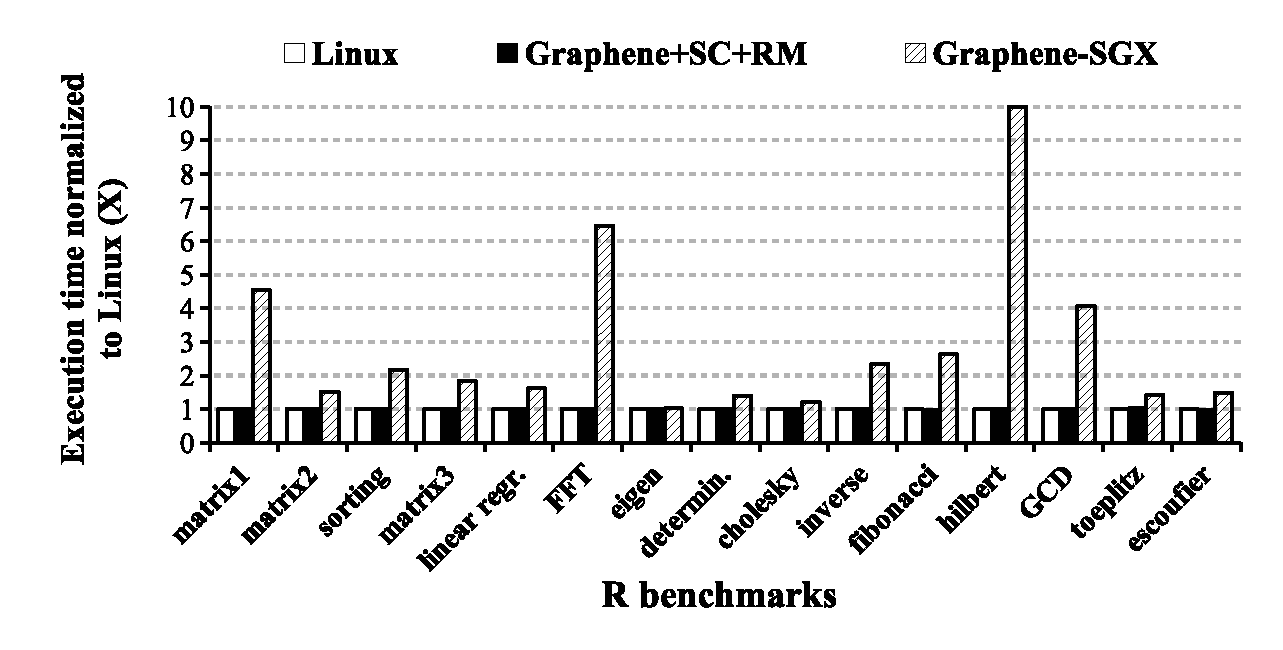
\includegraphics[width=\linewidth]{sgx/r-overhead}\\
{\bf (a) R}
\end{minipage}
\begin{minipage}{.275\textwidth}
\centering
\includegraphics[width=\linewidth]{sgx/gcc-overhead}\\
{\bf (b) GCC}
\end{minipage}
\begin{minipage}{.25\textwidth}
\centering
\includegraphics[width=\linewidth]{sgx/curl-overhead}\\
{\bf (c) CURL}
\end{minipage}

\caption{Performance overhead on desktop applications, including latency of R, execution time of GCC compilation, download time with CURL. The evaluation compares native Linux, \graphene{}, and \graphenesgx{}.} %{\bf Enclave creation time is deducted from the GCC execution time.}}
\label{fig:desktop-overhead}
\end{figure*}



\subsection{Command-Line applications}


We also evaluate the performance of a few commonly-used command-line applications.
%, to evaluate the performance of \graphenesgx{} on PCs instead of servers and clouds.
Three off-the-shelf applications are tested in our experiments:
{\bf R} (v3.2.3) for statistical computing~\cite{r-project}; {\bf GCC} (v5.4), the general GNU C compiler~\cite{gcc}; {\bf CURL} (v7.74), the default command-line web client on UNIX~\cite{curl}.
These applications are chosen because they are frequently used by Linux users,
and each of them potentially  be used 
in an enclave to handle sensitive data---either on a server or a client
machine.
% can realize profitable scenarios of using enclaves on desktop machines.



We evaluate the latency or execution time of these applications. 
%, because desktop users tend to care more about responsiveness than throughput.
In our experiments, both R and CURL have internal timing features to measure the wall time
of individual operations or executions.
%However, for other applications like GCC which does not include internal timing, evaluating the execution time can be influenced by many factors.
On a Linux host, the time to start a library OS is higher than a simple 
process, but significantly lower than booting a guest OS in a VM or
starting a container. 
Prior work measured Graphene (non-SGX) start time at 641 $\mu$s~\cite{tsai14graphene}, whereas starting an empty Linux VM takes 10.3s and starting a Linux (LXC) container takes 200 ms~\cite{agarwal15container}. 
%% dp; Note that this is MILLI seconds, not micro seconds.
%average memory footprint of an empty Linux VM, with memory deduplication, is about 96MB, . 


On SGX, the enclave creation time is relatively higher, \fixme{added more detailed number} ranging from 0.5s (a 256MB enclave) to 5s (a 2G enclave), which is a fixed cost that any application framework
will have to pay to run on SGX.
%For library OSes, the time for creating and initializing an enclave is not trivial, because it is similar to booting an lightweight OS.
% a significant part of the start-up time
% of an application is more significant, because creating enclaves is expensive.
%We consider the enclave creation time as a fixed cost for any application running in \graphenesgx{},
%and acceptable to users as long as it is responsive.
Enclave creation time is determined by the latency of the hardware and the Intel kernel driver, and is primarily a function of the size of 
the enclave, which is specified at creation time because it affects the enclave signature. %\fixmedp{although can't it grow with eadd?}.  
For non-server workloads that create multiple processes during execution,
such as GCC in Figure~\ref{fig:desktop-overhead},
the enclave creation contributes a significant portion to the execution time overheads, illustrated as a stacked bar.
%Since the enclave creation time is related to the enclave size, and unrelated to the workload,
%we deduct the enclave creation time from the execution time of GCC in Figure~\ref{fig:desktop-overhead}. \fixmedp{I think it might be better to show this as a stacked bar instead of just removing it.  Opaquely subtracting this cost doesn't seem right.  Let's discuss dp: I thought we agreed to change this...}

{\bf R}~\cite{r-project} is a scripting language often used for
data processing and statistical computation.
With enclaves, users can process sensitive data on an
OS they don't trust.
We use an R benchmark suite developed by Urbanek et al.~\cite{r-benchmark-25}, which includes 15 CPU-bound workloads such as matrix computation and number processing.
\graphenesgx{} slows down by less than 100\% on the majority of the workloads, excepts the ones which involve allocation and garbage collection: ({\tt matrix1} creates and destroys matrices, and both {\tt FFT} and {\tt hilbert} involve heavy garbage collection.)
Aside from garbage collection, these R benchmarks do not frequently interact with the host.
We further note that non-SGX \graphene{} is as efficient as Linux on all workloads, 
and these overheads appear to be SGX-specific.
%\fixmedp{Check this pontification}
In our experience, garbage collection and memory management code in managed language runtime
systems tends to be written with assumptions that do not match enclaves,
such as a large, sparse address space or that memory can be demand paged 
nearly for free (SGX version 1 requires all memory to be mapped
at creation); a useful area for future work would be to design
garbage collection strategies that are optimized for enclaves.
%we believe the overheads on \graphenesgx{} are contributed by enclaves.
 
{\bf GCC}~\cite{gcc} is a widely-used C compiler.
By supporting GCC in enclaves, developers can compile closed-source applications on customers' machines,
without leaking the source code.
GCC composes of multiple binaries, including {\tt cc1} (compiler), {\tt as} (assembler), and {\tt ld} (linker).
Therefore, GCC is a multi-process program using \syscall{execve}.
We test the compilation of thee source files with varied sizes,
using single C source files collected by MIT~\cite{gcc-benchmark}.
Each GCC execution typically \fixme{it's five, not four} creates five processes, and we run each process in a 256MB enclave by default.
%and has a fixed cost on enclave creation, which is unrelated to workload and depends on the enclave size.
%\fixme{check this}
\fixme{clarified this part, to prevent confusion between latency and overhead. also, GCC numbers got better.}
For a small workload like compiling {\tt gzip.c} (5 kLoC), running in \graphenesgx{} (4.1s) is 18.7$\times$ slower than Linux (0.2s).
The bulk of this time is spent in enclave creation, taking 3.0s in total, while the whole execution inside the enclaves, including initialization of the library OS and OS shield, takes only 1.1s, or 4.2$\times$ overhead.
For larger workloads like {\tt oggenc.c} (50 kLoC) and {\tt gcc.c} (500 kLoC), 
the overhead of \graphenesgx{} is less significant. % (3.6$\times$ and 2.1$\times$ overhead, respectively).
For {\tt gcc.c} (500 kLoC), we have to enlarge one of the enclaves ({\tt cc1}) to 2GB,
but running on \graphenesgx{} (53.1s) is only 2.1$\times$ slower than Linux (17.2s),
and 7.1s is spent on enclave creation.
%and the creation of four enclaves takes 8s.
%Each compilation has a fixed enclave creation time in \graphenesgx{}, which is about 1--2 seconds per enclave. We deduct the creation time of all enclaves  to gain more meaningful results, but do not hide rest of the overhead on fork.
%\fixmedp{Also not comfortable with this; add a bar?}
%In general, GCC in \graphenesgx{} is 1--5$\times$ slower than GCC on native Linux. 
%\fixmedp{This really needs some profiling if possible}
The overhead of non-SGX \graphene{} on GCC is marginal.
 



{\bf CURL}~\cite{curl} is a command-line  web downloader.
\graphenesgx{} can make CURL into a secure downloader that attests both server and client ends.
We evaluate the total time to download a large file, ranging from 1MB to 1GB, from another machine running Apache. % over Gigabit LAN.
%across high-speed university network\fixmedp{more specific, as above}.
\graphene{} has marginal overhead on CURL, and
\graphenesgx{} adds 7--61\% overhead to the downloading time of CURL, due to the latency of I/O.


\begin{figure*}[t!]
\centering

\begin{minipage}{.3\textwidth}
\centering
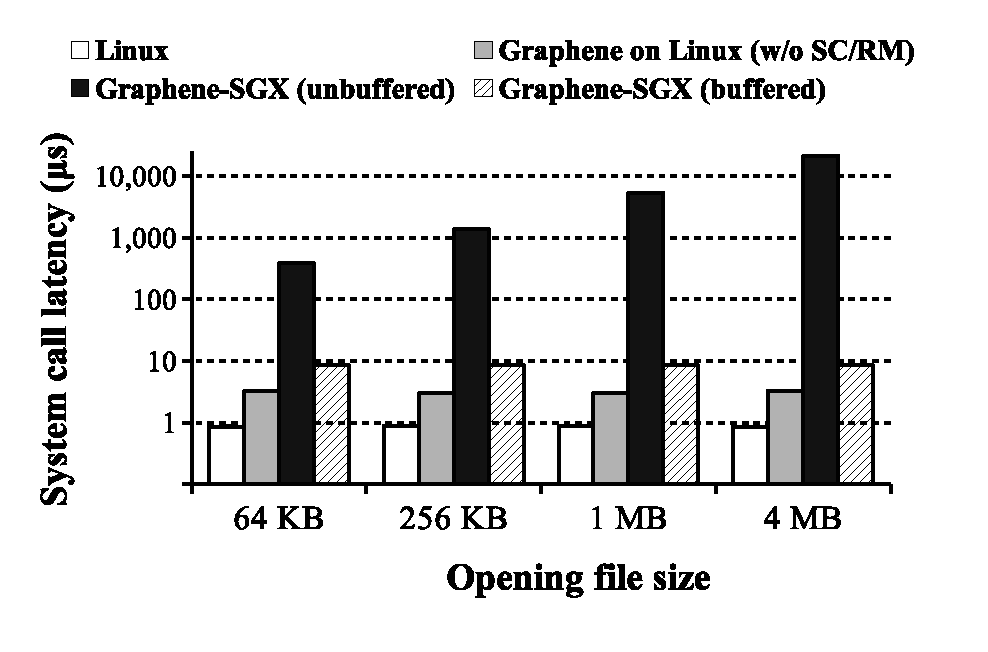
\includegraphics[width=\linewidth]{sgx/open-latency}\\
{\bf (a) Open a file}
\end{minipage}
\begin{minipage}{.3\textwidth}
\centering
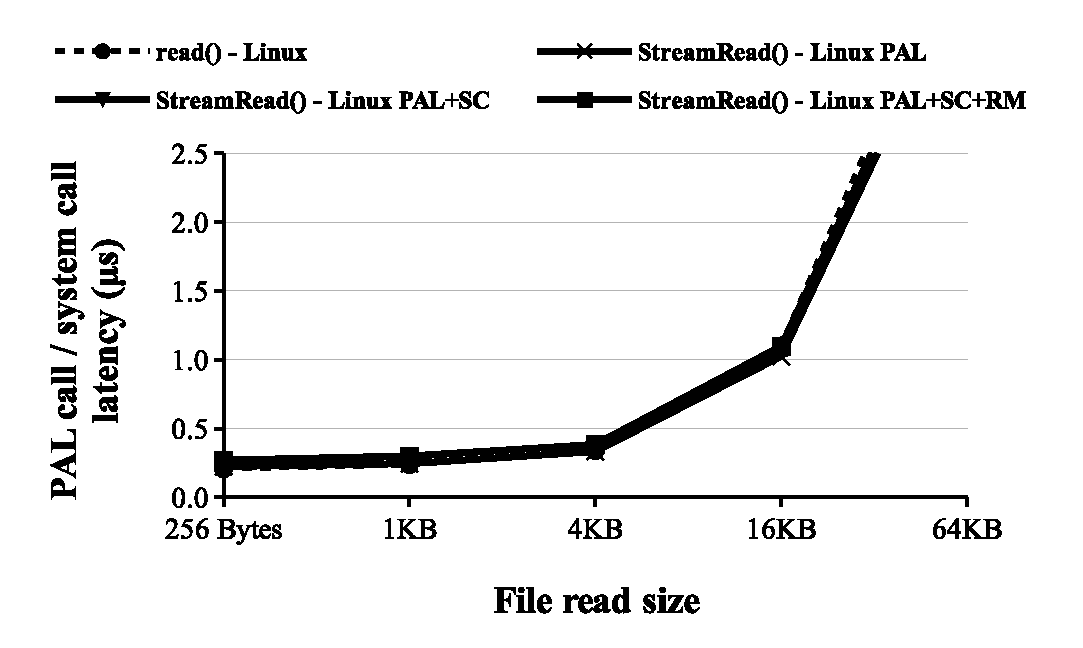
\includegraphics[width=\linewidth]{sgx/read-latency}\\
{\bf (b) Read a file}
\end{minipage}
\begin{minipage}{.3\textwidth}
\centering
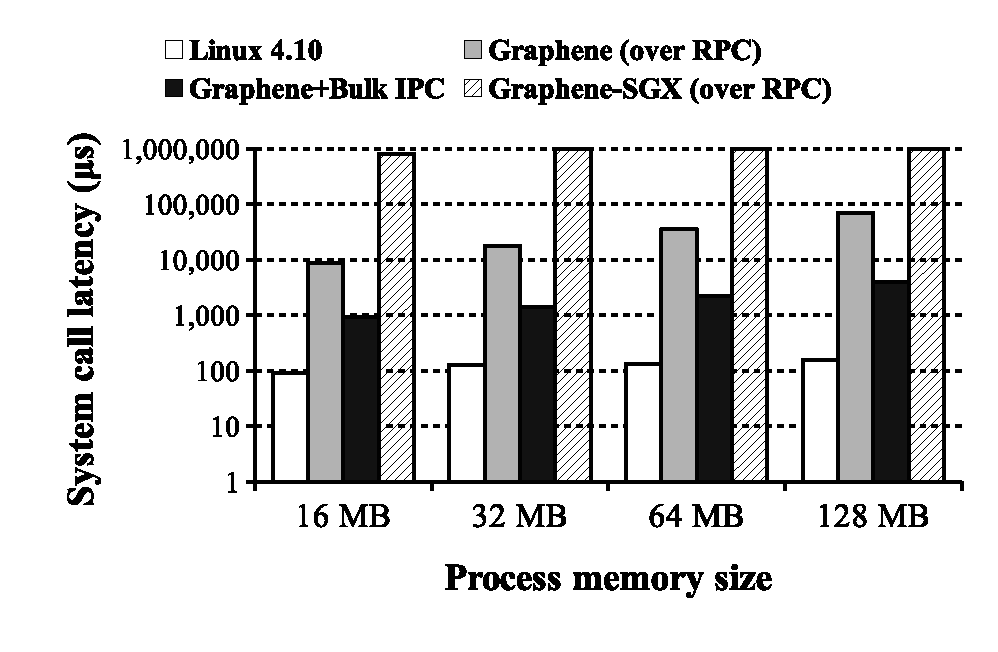
\includegraphics[width=\linewidth]{sgx/fork-latency}\\
{\bf (c) Fork a process}
\end{minipage}

\caption{Latency of some expensive system calls in \graphenesgx{}, including opening and reading a secured (authenticated) file, and forking a new process. The results are compared with native Linux and \graphene{}.}
\label{fig:syscall}
\end{figure*}


\subsection{Performance Overhead Analysis}


In this section we evaluate a few system operations that are heavily impacted by the \graphenesgx{} design.
%To shield dynamic loading and process creation,
%\graphenesgx{} uses computationally-expensive cryptographic techniques \fixmedp{more specific?} to verify enclave inputs.
% under the circumstance that the host OS cannot be trusted.
%As a trade-off to the security, the performance will be affected
%by additional cryptographic computation.
We measure the \syscall{open}, \syscall{read}, and \syscall{fork} system calls
using LMbench 2.5~\cite{McVoy:lmbench}.
A primary source of the overheads on these system calls is the cost of shielding applications, with run-time checks on the inputs.
Cryptographic techniques are used to: (1) validate the file against the secure hash, at \syscall{open}, (2) check the file chunks against the Merkle tree, at \syscall{read}, and (3) establish a TLS connection over inter-enclave RPC, at \syscall{fork}.
%opening a integrity-sensitive file for the first time, 
% or using cryptographic techniques, such as secure hashing, to verify the inputs.
% microbenchmarking specific system calls: 
% system calls,
%with different application settings.
%The microbenchmark is part of the LMBench 2.5 test suite
%\fixmedp{maybe merge this in the above paragraph, which feels a little coy}
%For instance, in order to shield dynamic loading, \graphenesgx{} checks each binary file against the secure hashes in the manifest,
%when the file is opened for the first time---after the whole file is copied into the enclave.
%\fixmedp{This happens after they are copied into enclave, memory right?}
%The verification happens when opening the file for the first time (often by the 
%After \graphenesgx{} validates the file, we generate a series of hashes of the file in chunks, as a merkle tree.
%to prevent verifying the whole file again when later randomly reading a part of the file.
%\fixmedp{So is this for the case when a file is swapped out?  I'm confused here - some details are missing}
%The latency of opening and reading an authenticated file in \graphenesgx{} is dominated by SHA256 and SHA512 calculation.
The remaining overheads contribute to exiting the enclave for host system calls, and bringing memory into the EPC (enclave page cache) or decrypting 
memory on a last-level cache miss. %and later the cache where the memory is decrypted by the CPU.


Figure~\ref{fig:syscall}(a)
shows the overhead for authenticating files in \syscall{open}.
\fixme{change overhead to latency}
Depending on the file size, the latency of \syscall{open} on \graphenesgx{} is 383$\mu$s (64KB file) to 21ms (4MB file), whereas on Linux, the latency is constant at 0.85$\mu$s.
We note that this is where enclaves are at a disadvantage, as \syscall{open} 
normally does not need to read file content; whereas here \graphenesgx{} uses \syscall{open}
as a point at which to validate file content.
For a subsequent \syscall{open}, when the Merkle tree is already generated, the overhead of simply exiting enclave for \syscall{open}, and searching the file list in the manifest, is about 9$\times$.
%\fixmedp{why?}


One might be able to optimize further for cases where only part of a file is accessed
with incremental hashing.  However, in the common case where nearly all of the file is accessed,
these costs are difficult to avoid when host file system is untrusted.
Another opportunity 
is to create the Merkle tree offline, when the manifest is created.
%\fixmedp{I think the second idea has legs...}


%This is an inevitable cost, because normal \funcname{open} on trusted OSes
%need not to access file content.
%After verifying the file, \graphenesgx{} buffers the chunk hash values, to skip whole-file verification when the file is reopened.

Figure~\ref{fig:syscall}(b)
shows the overhead for authenticating files in \syscall{read}, which 
is lower than \syscall{open}.
Since the whole file has been verified at \syscall{open}, the sequential \syscall{read} only verifies the chunks of files it is reading from untrusted memory.
%Reads from data cached in enclave memory are cheaper.  %\fixmedp{right? can we say how much cheaper?  Maybe add separate bars for both cases?}
% Therefore, \syscall{read} is actually much cheaper than \syscall{open}.
Depending on the size of blocks being read, the latency on \graphenesgx{} is 0.5$\mu$s (64-byte \syscall{read}) to 16.9$\mu$s (4KB \syscall{read}). The latency of \syscall{read} on Linux is \roughly{}0.1$\mu$s for any block size below 4KB.
If the file is not authenticated,
\graphenesgx{} only copies the file contents into the buffer, and the overhead reduces to 48\% (64-byte \syscall{read}) to 83\% (4KB \syscall{read}).
\fixmedp{Consider doing larger buffers, say up to 64k or even 4 MB}

%\fixmedp{In the legend for 7b, unsecure should be insecure}


Figure~\ref{fig:syscall}(c) shows the overhead of forking a process.
As described in \ref{sec:multiproc}, the latency of \syscall{fork} in \graphenesgx{} is affected by three factors:
creation of a new enclave, local attestation of the integrity, and duplicating the process state over an encrypted RPC stream.
Combining these factors, \syscall{fork} is one of the most expensive calls in \graphenesgx{}.
%, but at least it is supported natively on the current hardware.
The default enclave size is 256MB.
%which takes \roughly{}0.5s to create. 
Our evaluation shows that the latency of forking a process is around 0.8s (16MB process) to 2.7s (128MB process), but can be more expensive if the parent process uses more memory.
The trend matches the performance of \graphene{} without the bulk IPC optimization.
\fixmedp{If you want, some thoughts on how this might be improved in the future would be nice...  One good suggestion is recycling enclaves, or pre-forking so measurements can be done in parallel}
%Due to the overhead on \funcname{fork}, \graphenesgx{} is not suitable for fork-intensive workloads like Bash scripts
%if performance is critical.

\fixme{talk about a limitation of improving fork. check this.}
One way to further optimize \syscall{fork} is to reduce or avoid enclave creation time; one can potentially pre-launch a child enclave, and then migrate the process contents later when \syscall{fork} is called.
There might be another opportunity to improve the latency of process migration,
if copy-on-write sharing of enclave pages can be supported in future generations of SGX.
%Unfortunately, sending the process contents is difficult to avoid in \syscall{fork},
%as SGX disallows sharing enclave memory between multiple enclaves.

%\fixmedp{I assume 5.4 isn't done yet}



\subsection{TCB Size and Shielded Functionality}

In this section we measure the increase in TCB size of \graphenesgx{},
%in lines of code, 
as well as 
%compare the TCB size increased by \graphenesgx{} to an unmodified application, in lines of code, and 
the OS functionality shielded by the framework.
We compare to \scone{} and \panoply{}, using
%For SCONE and Panoply, we use 
numbers reported in their papers. 
%The conventional One generally assumes 
A smaller TCB is generally easier to review or possibly verify,
and is assumed to have fewer vulnerabilities.
%more implies lower burden for code review or formal verification, and less risk of writing exploitable code.
%For instance, Panoply argues that, because its use cases are typically smaller than 20kLoC, including both the application logic and Panoply itself, it is within the realm of future, automated verification~\cite{shinde17panoply}.

\fixmedp{Reviewer B asks for memory footprint, which isn't a bad idea}

\begin{table}
\footnotesize
\centering
\bgroup
\def\arraystretch{1.2}
\setlength{\tabcolsep}{0.5em}
\begin{tabular}{>{\raggedright\arraybackslash}p{9em}>{\raggedleft\arraybackslash\bf}p{7em}>{\raggedleft\arraybackslash}p{4.25em}>{\raggedleft\arraybackslash}p{4.25em}}
Components                    & \graphenesgx{}  & \scone{}     & \panoply{}  \\
\hline
libc (ld, libm, pthread)      &  1,292 &   88 & --      \\
                              & (glibc-2.19) & (musl)   &          \\
Library OS                    &     34 &  --      & --     \\
PAL / OS Shield               &     22 &   99 & 10  \\
\hline
Total                         &  1,348 &  187 & 10  \\
\hline
\end{tabular}
\egroup
\caption{TCB size (in thousands of lines of code) of \graphenesgx{}, \scone{}, and \panoply{}.}
\label{tab:tcb-size}
\end{table}

Table~\ref{tab:tcb-size} lists the lines of code in each components within the TCB of \graphenesgx{}, \scone{}, and \panoply{}.
By comparing the total TCB size, \graphenesgx{} is 9$\times{}$ larger than \scone{}, and 134$\times{}$ larger than \panoply{}.
However, the primary difference is the selection of libc: 
for maximum compatibility, \graphene{} uses glibc.
\scone{} uses the smaller musl libc, which lacks some features of glibc.
%it would be easy to use the smaller, and incomplete, musl libc.
%SCONE uses 
% Linux applications, \graphenesgx{} chooses to use a minimally-modified glibc, whereas SCONE uses the much more lightweight musl and 
\panoply{} excludes libc from its TCB,
% \fixmedp{what is their rationale, again? Check this}
to fit into the range of automated formal verification,
as they shield at the libc interface.
In principle, \graphene{} could easily support musl as well as glibc for applications
that do not need the additional features of glibc.
We also see the benefit of removing unused code from 
libraries, especially in an unsafe language,
similar to the approach taken in unikernels~\cite{unikernels}.
On balance, 
this choice of libc implementation is largely orthogonal to the issue
of how general-purpose the shields are.

%We argue that the choice of libc is orthogonal to the design of \graphenesgx{}; one can statically compile the applications against musl or glibc if TCB size is a concern, or given plenty of time, trim the libc functionality to bare minimum. 

If we focus on the TCB size of the library OS and the shields, 
\graphenesgx{} is 
%library OS and PAL in \graphenesgx{}, with the shielding layer of SCONE, we are 
44\% smaller than \scone{}. 
We cannot analyze the size of \scone{} because it is closed source.
%, although
%we suspect
%Although it is unclear what is in the implementation of SCONE, because it is not yet open-sourced, we believe the largest portion of their TCB contributes to the cryptography library.
\panoply{} has a smaller TCB in its shield, but within the same order of magnitude.
Panoply only shields 91 out of 256 supported POSIX functions; for context, POSIX 1003.1 defines 1,191 APIs~\cite{POSIX1003-1-2008}.
%out of 256 currently supported by \panoply{} \fixmedp{The better number is how many total functions in POSIX}.

All three of these compatibility layers or shields are within the same
order of magnitude in code size, and the differences are likely 
correlated with different ranges of supported functionality.
A recent study indicates that only order-of-magnitude differences in code
size correlate with reported CVE vulnerabilities; within the same order-of-magnitude,
the data is inconclusive that there is a meaningful difference in risk~\cite{security-metric}.
Thus, increased generality does not necessarily come with 
increased risk. % is not a clear relationship between risk 

% data only correlates
%with differences in code size when 

%Besides the choice of libc, we argue that the TCB size of a library OS or a shim shielding layer is actually correlated with the functionality that it supports or shields. Because none of the three frameworks have completely shielded the whole Linux system call table or POSIX, it is unclear how much code has to be added in the future. \graphenesgx{} also shows that one can always engineer a library OS with a small TCB, if most code is not reused from a monolithic OS kernel like Windows or Linux.
%A recent study of the CVE database also points out that having a larger TCB does not necessarily indicate more vulnerabilities, even when the difference is more than two order-of-magnitude. 



\input{apistudy}

\makeatletter
\def\input@path{{}}
\makeatother
\graphicspath{{}}
\section{Summary}



The Linux PAL successfully leverages a limited subset of Linux system calls,
to implement the whole PAL ABI for running a
full-featured \libos{}.
\Thehostabi{} separates the development of a host OS or hypervisor
from the complexity of emulating a sufficiently-compatible
Linux kernel.
The chapter shows that most calls in \thehostabi{}
can be directly translated to similar system calls on a Linux host kernel.
Only a few \hostapis{}, such as process creation and inter-thread synchronization, require additional attention for developing an efficient implementation strategy.



The Linux PAL also enforces robust security isolation
between mutually-untrusting applications,
by placing applications in separate, VM-like sandboxes.
The security isolation on a Linux host is based on system call restriction using a \seccomp{} filter, and a trusted reference monitor. % for checking resource access.
Security isolation at the host interface
restricts an untrusted application to explore vulnerable execution paths
inside a Linux kernel.
A \seccomp{} filter 
enforce a fixed, minimal system call profile, regardless of bloated dependency of an application.
The reference monitor follows
simple, white-listed manifest rules listing 
all the authorized files and network addresses of an application,
using well-known semantics
such as AppArmor~\cite{apparmor} or iptable-like firewall rules~\cite{iptablesman}.
The reference monitor can further enforce dynamic, process-specific isolation by splitting a sandbox
to run a child \picoproc{} under more restricted
resource permissions.
\graphene{} on a Linux host can serve as a sandbox framework
with a reduced attack surface
upon the host kernel.









\makeatletter
\def\input@path{{}}
\makeatother
\graphicspath{{}}

\section{System API Study}

%\fixmedp{I am not sure about this paragraph.  I probably need to discuss in person} \fixmebj{any better?}

Concurrent with our work, Atlidakis et al.~\citep{atlidakis16posix} conducted a similar 
study of POSIX.
A particular focus of the POSIX study is measuring fragmentation across different POSIX-compliant OSes
(Android, OS X, and Ubuntu), as well as identifying points where higher-level frameworks
are driving this fragmentation, such as the lack of a ubiquitous abstraction for graphics.
Both studies identify long tails of unused or lightly-used functionality in OS APIs.
The POSIX study factors in dynamic tracing, which can yield performance insights;
our study uses installation metrics, which can yield insights about the impact of incompatibilities end-users.
Our paper contributes complimentary insights, such as a metric and incremental path for 
completeness of an emulation layer, as well as analysis of the importance of less commonly-analyzed 
APIs, such as pseudo-files under {\tt /proc}.

%% \fixmetsai{My crack on discussing this work.}
%% Atlidakis, et. al use a related technique of static analysis,
%% to trace POSIX API linkage in multiple OSes such as Android, OS X and Ubuntu.
%% The study also uses dynamic analysis, as to intercept applications' runtime API usage using a library called {\tt libtrack},
%% to trace dynamic invocation of POSIX abstractions in 45 popular Android applications.
%% While our work is focused on
%% studying more universal, modern Linux API importance to end users on a large scale,
%% their study targets on elaborating the dependency on POSIX APIs
%% in applications,
%% and more importantly,
%% the performance implications of POSIX APIS to application in the runtime.

A number of previous studies have investigated how other portions of the Operating System
interact, often at large scale.
Kadav and Swift~\citep{understand-drivers} studied the effective API the Linux kernel exports 
to device drivers, as well as device driver interaction with Linux---complementary to our study
of how applications interact with the kernel or core libraries.
Palix et al.\ study faults in all subsystems of the Linux kernel and identify the 
most fault-prone subsystems~\citep{linux-faults}.
They find architecture-specific subsystems have highest fault rate, followed by file systems.
Harter et al.~\citep{file-not-file} studied
 the interaction of a set of Mac OS X applications with the file system APIs---identifying a number
of surprising I/O patterns.
%Other systems have studied specialized set of software that 
%interact with specific components of Linux kernel.
%%For instance, Harter et.al. study only I/O behavior of iBench applications on Mac to conclude that each of these applications form a mini-filesystem amongst themselves and their interactions with the
%filesystem kernel component are different than other standard applications~\citep{file-not-file}.
%Another study of device drivers classifies drivers into 5 different classes after analyzing the interacion of the drivers with the kernel, devices, and buses~\citep{understand-drivers}.
%SymDrive identifies busgs in device drivers in the kernel by studying I/O changes after the driver patches~\citep{symdrive}. \fixmedp{Is this really related?  I was thinking of a different swift paper}
Our approach is complementary to these studies, with a focus on overall API 
usage across an entire Linux distribution.

%% Our study however is more general as 
%% we focus on all the applications in the Debian/Ubuntu repositories
%% and the applications' use of different kernel interfaces including the 
%% standard system calls, vectored system calls and other interfaces such as
%% /proc, /sys and /dev.


%\note{about 1/2 page}

A number of previous studies have drawn inferences about user and developer behavior
using Debian and Ubuntu package metadata and popularity contest statistics.
Debian packages have been analyzed to study the evolution 
of the software itself~\citep{macro-study, life-death, mining-over-time}, 
to measure the popularity of application programming 
languages~\citep{upgrade-libre}, to analyze dependencies between the packages~\citep{package-dependency}, 
to identify trends in package sizes~\citep{pigs-to-stripes}, 
the number of developers involved in developing and maintaining a package~\citep{toy-story},
%\fixmedp{right?}\fixmebj{yeah}, 
and estimating the cost of development~\citep{measuring-woody}.
Jain et al.\ used popularity contest survey data to 
prioritize the implementation effort for new system security policies~\citep{jain14setuid}. % \fixmebj{nice one :)}.
This study is unique in using this information to infer the relative importance of 
of system APIs to end users, based on frequency of application installation.

%%% Although our study is unique in its focus on footprint of interaction
%%% between the applications and the kernel interfaces, a body of similar application studies
%%% exist that analyze different questions than the ones discussed in this paper. 

%%% On the other hand, we analyze the Debian and Ubuntu package repositories to 
%%% study the kernel interface footprints of the applications
%%% and the minimal set of interfaces necessary to support those applications.

%\fixmedp{How do these studies quantify compatibility?}
A number of previous projects develop techniques or tools to identify software incompatibilities, with 
the goal of avoiding subtle errors during integration of software components.
The Linux Standard Base (LSB)~\citep{linux-standard-base} 
predicts whether an application can run on a given distribution based on the 
symbols imported by the application from system libraries.
%exported symbols and libraries provided by that distribution.
%examines
%applications to get the binary symbols and libraries used by those applications.
%LSB goal is
%Several previous studies have examined compatibility of different software library implementations~\citep{linux-standard-base}
Other researchers have studied application compatibility 
across different versions of same library,
creating rules for library developers
to maintain the compatibility across versions~\citep{shared-library}.
Previous projects have also developed tools to verify backward compatibility of libraries, based on checking for any changes in library variable 
type definitions and function signatures~\citep{backward-compatibility}.
%that can cause backward binary compatibility problems
Another variation of compatibility looks at integrating independently-developed components of a larger software project; 
solutions examine various attributes of the components' source code, such as recursive functions and strong coupling of different classes~\citep{component-compatibility}.
In these studies, compatibility is a binary property, reflecting a focus on correctness. Moreover, these studies are focused on the interface between the application and the libraries or distribution ecosystem.
In contrast, this paper proposes a metric for relative completeness of a prototype system. % with a focus on the compatibility between the applications or libraries and the kernel ABIs.


%%% Research has been done on the compatibility of components during software development~\citep{component-compatibility}.
%%% There are verifiers for compatibility
%%% between software components such as binaries and libraries based on
%%% broad spectrum of compatibility problems~\citep{backward-compatibility}.
%%% Other studies focus on compatibility of application binaries with the different 
%%% versions of libraries~\citep{shared-library} and with libraries provided in different 
%%% distribution environments~\citep{linux-standard-base}.
%%% However, we study the kernel-userspace ABI compatibility between the application binaries
%%% and systems that support linux ABI.

%\fixmedp{I'm not sure what the theme of this paragraph is.  Everything is listed here, but it is pretty terse.
%I like to frame each paragraph as ``what is known'', ``how it has been used'', and ``what is new here'' (and maybe why important)}
%\fixmebj{This paragraph is about all the related work that does any sort of system call profiling for applications and what do they do with it.}

Identifying the system call footprint of an application is useful for a number of reasons;
our work contributes data from studying trends in system API usage in a large set of application software.
The system call footprint of an application can be extracted by static or dynamic analysis.
The trade-off is that dynamic analysis is easier to implement quickly, but the results are input-dependent.
Binary static analysis, as this paper uses, 
can be thwarted by obfuscated binaries,
which can confuse the disassembler~\citep{zhang13cfi}.
%is also subject to the limitations of the disassembler to deal with
Static binary analysis has been used to automatically generate application-specific sandboxing 
policies~\citep{policy-extraction}.
Dynamic analysis has been used to compare system call sequences of two applications
as an indicator of potential intellectual property theft~\citep{software-theft},
to identify opportunities to batch system calls~\citep{multi-call},
to model power consumption on mobile devices~\citep{power-modelling},
and to repackage applications to run on different systems~\citep{cde}.
These projects answer very different questions than ours, but could, in principle, benefit
from the resulting data set.

%Many previous works have used static as well as dynamic analysis of applications to determine the system calls that they use.
%While dynamic analysis is the easiest to get a system call trace of the applications, it is very difficult to guarantee that all branches in the code
%are exercised. On the other hand while static analysis can cover the complete binary, we share the same assumption as other static analysis solutions that the application is not obfuscated.
%Researches have used static analysis to identify system call footprints of applications to automatically generate application-specific sandboxing policies
%% Others have also used dynamic analysis to determine and compare system call sequences within applications to detect software threat assuming that common system call sequences may imply
%% common or stolen code~\citep{software-theft}.
%% \fixmedp{I don't get this one---a little more detail please?}\fixmebj{how about now?}
%% Another work reduces the number of kernel boundary crossings by replacing group of system calls, that are identified by dynamically profiling applications, with a single system call~\citep{multi-call}.
%% %and optimize the performance by clustering multiple related system calls~\citep{multi-call}\fixmedp{or this one?}.
%% Runtime system call tracing of applications has also been used to model 
%% fine-grained power consumption for Smartphones~\citep{power-modelling}.
%% CDE~\citep{cde} use system call information of x86 Linux 
%% programs to package them differently to run on other x86 Linux machines.
%% All these research works can benefit from our study and can be applied to large number of applications in the Ubuntu repository.
%% Moreover, our study answers a different question of what fraction of these packages
%% can be compatible to a Linux ABI based system.

 



%\declarecommand{\dentry}{dentry}
\declarecommand{\dentries}{dentries}
\declarecommand{\Dentry}{Dentry}
\declarecommand{\Dentries}{Dentries}
\declarecommand{\vnode}{{\tt vnode}}
\declarecommand{\vnodes}{{\tt vnodes}}
\declarecommand{\dcache}{{dcache}}
\declarecommand{\inode}{{inode}}
\declarecommand{\dnlc}{{\tt DNLC}}
\declarecommand{\fnone}{{X}}
\declarecommand{\fntwo}{{Y}}
\declarecommand{\fnthree}{{Z}}
\declarecommand{\fnfour}{{A}}
\declarecommand{\fnfive}{{B}}
\declarecommand{\fnsix}{{C}}
\declarecommand{\lnone}{{L}}
\declarecommand{\lntwo}{{R}}
\declarecommand{\completeflag}{{\tt DIR\_COMPLETE}}
\declarecommand{\lookupflag}{{\tt NEED\_LOOKUP}}

\declarecommand{\ubuntuver}{{14.04}}
\declarecommand{\linuxver}{{3.14}}
\declarecommand{\prefixcheckcachesize}{{4}}
\declarecommand{\PCCsize}{{64 KB}}
\declarecommand{\lookuptablesize}{{64}}
\declarecommand{\lookuptableway}{{2}}

\declarecommand{\statspeedup}{{26}}
\declarecommand{\openspeedup}{{13}}
\declarecommand{\slowpathcost}{{xx}}
\declarecommand{\dentryoldsize}{{192}}
\declarecommand{\dentrynewsize}{{192}}
\declarecommand{\dentrysizeoverhead}{{64}}
\declarecommand{\dovecotspeedup}{{12}}
\declarecommand{\gitspeedup}{{7}}
\declarecommand{\updatedbspeedup}{{29}}

\newcolumntype{L}[1]{>{\raggedright\let\newline\\\arraybackslash\hspace{0pt}}m{#1}}
\newcolumntype{C}[1]{>{\centering\let\newline\\\arraybackslash\hspace{0pt}}m{#1}}
\newcolumntype{R}[1]{>{\raggedleft\let\newline\\\arraybackslash\hspace{0pt}}m{#1}}

\chapter{Optimizations in Legacy Operating Systems}
\label{chap:dcache}

This chapter describes the formal definition of the \graphene{} host ABI.

\section{Basic Definitions}

The \graphene{} host ABI defines a set of {\em functions}, similar to the API of UNIX or POSIX.
The functions are directly called by the library OS, along with the arguments given either in the registers or on the stack.
A host-specific \graphene{} loader is responsible for resolving the linking, from the library OS to the host ABI.
\papersection{Challenges for Partitioning with Enclaves}
\label{sec:background}
In this section, we will give a brief overview of \sgx{}, and discuss 
the key challenges developers face when trying to manually partition applications using a technology such as \sgx{}.
%discuss the programming models and threats to security of \sgx{} enclaves.

\papersubsection{Background on \intel{} \sgx{} Enclaves}

\intel{} \sgx{} ({\it Software Guard Extension})
is a set of new x86/x64 instructions
introduced in the \intel{} Skylake processor family.
Using \sgx{}, an 
application can designate part of its virtual memory as an {\em enclave}.
The CPU guarantees that the contents of the enclave never leave the CPU package unencrypted.
The CPU also measures the integrity of a binary loaded into the enclave, and offers remote attestation,
similar to a TPM\fixmedp{cite}.

%%% create a protected memory region, called an {\em enclave}, inside it's virtual memory,
%%% where it can load its security sensitive data with hardware-enforced isolation from the untrusted OS. 
%%% The processor with \sgx{}
%%% guarantees that any data loaded in enclave
%%% stays encrypted in the DRAM, by using a secret key deterministically derived from the application's cryptographic measurement and the CPU secret. 

\sgx{} is an appealing tool for protecting small amounts of highly-sensitive data or code, because it can defend 
against a malicious or compromsed OS, hypervisor, or even hardware peripheral.
For instance, \fixmedp{Foo} et al.~\fixmedp{cite that \sgx{} workshop paper} show how \sgx{} can be used
to build a trusted path from a video chat application to a GPU and network card, which maintains confidentiality and integrity of the
video stream, even if the OS is compromised.
Simlarly, because DRAM contents are encrypted, \sgx{} can resist cold-boot attacks~\cite{halderman09coldboot} or 
malicious peripheral devices~\cite{hudson15thunderstrike}.


%%% \sgx{} also proves the integrity of loaded binaries to remote trusted entities
%%% using mutual attestation based on a symmetric key generated from the measurements of communicating entities.
%%% \sgx{} usage model mostly involve the launched enclave mutually attesting the trusted host
%%% to obtain provisioning of security-sensitive information
%%% through a trusted channel. Such an execution model leverages resources such as CPU and DRAM from vulnerable untrusted \sgx{}-enabled hosts owned by cloud providers
%%% by extending the trust from
%%% the hosts owned and trusted by the clients or service providers.
%%% For instance, \sgx{} can isolate the decoder engine in an enclave
%%% after authenticating the customers to enforce Digital Right Management (DRM) even if the digital data is hosted on an untrusted cloud server.

%Use cases of \sgx{} mostly involve the launched enclave
%retrieving a cryptographically signed attestation from the processor,
%to exchange security critical information with remote servers through secured channels.
%The effect is equivalent to expanding the trusted space from remote servers
%to the local end, to harness local resources such as CPU and DRAM.

%One must note that \sgx{} only promises the integrity of application binaries
%initially loaded in enclaves.
%The gap between integrity of binaries and complete security has to be filled
%by ones who develop and approve the applications.
%More specifically, the clients are responsible of
%testing whether the applications contain any vulnerabilities
%that lead to information leak.
%To minimize the risk of leaving any flaws in the applications unintentionally,
%developers often tend to cut down the trusted computing base (TCB)
%of the applications. With smaller TCB, clients who launched the enclaves
%can more easily reason about the thoroughness of securing the execution.

%%% The key strength of \sgx{} enclaves over other software-based isolation framework such as
%%% {\em Flicker}, {\em Inktag} or {\em Virtual Ghost} is
%%% the ability to defend against attacks at the hardware level.
%%% These software-based solution often
%%% rely on a hypervisor below the OS to isolate the applications.
%%% If the hardware is attacked,
%%% the attackers may still bypass the software checkpoints,
%%% or directly steal confidential information from the DRAM.
%%% For \sgx{}, the only hardware included in the TCB is the CPU package,
%%% and in practice CPUs are believed to be hard to attack.
%%% Using techniques like cold-boot attacks~\cite{halderman09coldboot}
%%% to peek into DRAM content,
%%% or intruding the boot process using corrupted peripheral devices like Thuderstrike~\cite{hudson15thunderstrike}
%%% will affect any software-based isolation, but not \sgx{} enclaves.

\paragraph{Non-Partitioned Applications.}
One approach to using \sgx{} is to run an entire application in the enclave.
This is exemplified by Haven~\cite{baumann14haven}, which runs a \win{} application and all supporting libraries
on top of a {\em library OS}.  This approach is illustrated on the left side of Figure~\ref{fig:libosvssdk}.
The library OS approach does not require any application changes, but bloats the TCB \fixmedp{Rough number of how big Haven is}.
By pulling millions of lines of extraneous code into an enclave, there is a significantly increased risk 
of vulnerabilities that disclose
sensitive data, such as Heartbleed~\fixmedp{cite}.
The library OS approach is useful in its simplicity of deployment and can provide practical benefits, 
such as protecting an application from an untrusted cloud hypervisor.

\begin{figure}[t!]
\centering
\includegraphics[width=\linewidth]{figures/libosvssdk.pdf}
\footnotesize
\vspace{-0.2in}
\caption{
Comparison between the libOS-based model (e.g., Haven)
and the partitioned model for programing applications in enclaves.
Green (light) boxes are trusted components and red (dark) boxes are untrusted.
The libOS-based model yields a larger TCB in the enclave,
while the partitioned model requires developers to be responsible for determining the untrusted interface at the enclave boundary.
}
\label{fig:libosvssdk}
\end{figure}


This paper focuses on a second usage model for enclaves, where the application is partitioned into
untrusted and one or more trusted components (right side of Figure~\ref{fig:libosvssdk}).
Sensitive data and computation are placed inside of enclaves.  This approach requires the developer to
identify sensitive code and data; design and harden an interface between trusted and untrusted components; 
modify the application source; and reason about potential information flows at the enclave boundary.
This effort can be non-trivial and subtle, but for application developers motivated by interests such as 
regulatory compliance or competitive advantage in business, the additional effort can yield a much smaller trusted computing
base (TCB), and thus a reduced attack surface.
A key goal of \sysname{} is to minimize the developer's effort to partition an application---both in lines of 
code changed, and in leveraging language analysis to reason about narrow points in the application's data and control flow.


%To achieve smaller TCB, the software development kit of \sgx{}
%intends to encourage developers to partition the applications and
%keep only security sensitive components in the enclaves.
%Such an intention is exactly contradicted by the trust model of \haven{},
%which must trust the loaded application as a whole.
%Except for the cases in which the whole applications must be secured,
%\haven{} actually downgrades the trustworthiness of enclaves.
%Figure~\ref{fig:libosvssdk} shows the comparison of the two models.

%%% In prior works using \sgx{} enclaves to secure applications,
%%% developers choose between two different programing models: the {\em library-OS-based} and the {\em partitioned} model (as shown in Figure~\ref{fig:libosvssdk}).
%%% In the libOS-based model, developers run the whole standalone,
%%% legacy application inside the enclave, using library OS such as {\em Haven} or {\em Graphene libOS} to facilitate the rich OS features.
%%% The main benefit of using library OS is that developers only have to employ minimal efforts to port any existing application.
%%% Even when designing new applications, developers bear no responsibility
%%% of identifying and reasoning about
%%% the security sensitive part of the application.

%%% However, when using libOS-based model, a sophisticated legacy application
%%% will yield huge trusted computing base (TCB) in the enclave,
%%% aggravating the risk of leaking information through vulnerabilities inside the enclave.
%%% Known bugs such as {\em the heart-bleeding bug} has shown that
%%% running security sensitive code like an encryption engine, and management code such as heart-beating service in the same address space
%%% can cause vulnerabilities that compromise the security by leaking the encryption key.
%%% As a result, using a partitioned model, developers can isolate only the most security sensitive components in an enclave,
%%% and leave the remaining code outside to minimize the TCB.

%%% Developers have to define the {\em untrusted interface} 
%%% to allow parts of a partitioned applications to interact.
%%% The untrusted interface is used either by the the untrusted components
%%% to trigger execution of the isolated components,
%%% or by isolated components to use untrusted rich OS features, such as networking for provisioning and sending the execution output to the remote hosts.
%%% Unlike the libOS approach that has a fixed untrusted interface (for different applications) at their interaction boundary with the OS,
%%% the width of untrusted interface for a partitioned application is up to developers' design.
%%% The \intel{} SDK for \sgx{} supports a set of syntaxes to specify the type and direction of flow for parameters of the untrusted interface, and enforces primitive
%%% type-checking of incoming values on transition to enclave.

%%% The trade-off between the libOS-based and partition model is based 
%%% on ease of development, the width of untrusted interface,
%%% and size of TCB.
%%% The benefit of the libOS-based model is that developers can save the effort
%%% of determining what to execute in the enclave,
%%% and whether the execution is safe,
%%% because the whole application is wrapped in the enclave.
%%% However, the risk of having vulnerabilities in the applications
%%% is not reduced, but in fact amplified due to the addition of
%%% the library OS (e.g., the Haven binary yields around a few hundred MBs) to TCB.
%%% On the other hand, if the developers are willing to spend effort on carefully identifying the untrusted interface and re-designing their application around this interface, the partitioned model can improve security guarantees by minimizing the attack vectors.

%%% The goal of \sysname{} is to provide the benefits of both models.
%%% \sysname{} support a partitioned model
%%% for developers to isolate security-sensitive part of a \java{} application in enclave,
%%% and provide a language-based tool to automatically partition
%%% the minimal supporting classes to generate the enclave image.
%%% Even in the case where the isolated component need to frequently interact with the untrusted component or the OS,
%%% the language protection technique of information flow tracking
%%% guarantees that the secrets in the enclave are never leaked
%%% without the developers explicit consent. 

\paragraph{Side Channels and Denial-of-Service.}
In the current \sgx{} design, side channels are a signficant concern for either the library OS or partitioned model, and are out of the scope of this paper.
A controlled channel attack~\fixmedp{cite} can single step enclave execution by inducing page faults
in the enclave.  \sysname{} does not specifically defend against side channel attacks,
and we expect that any solution to this problem involves redesigning the division of labor in virtual
memory management for enclaves.

Similarly, there is no guarantee that a compromised application will ever enter
an enclave.  Denial-of-service attacks are out of scope for this paper.


\papersubsection{Challenges for Application Partitioning on \sgx{}}

\sgx{} provides useful building blocks for secure applications, but does not
absolve the programmer of any responsibility for reasoning about end-to-end security.
Bugs in the application or supporting libraries can still disclose sensitive data from an enclave,
and porting code into \sgx{} can be subtle.
This subsection outlines several pitfalls in partitioning an application for \sgx{}.

%%% \sgx{} enclaves provide strong isolation guarantee for applications,
%%% against the malicious or vulnerable application components, system stack,
%%% and hardware (except the CPU itself).
%%% However, the security guarantees of the \sgx{} enclave is dependent on whether the developers design perfect applications without exploitable vulnerabilities that may compromise the application's security.
%%% As the application developers are not perfect,
%%% even applications or components isolated in enclave can face threats to their security.
%%% As follows, we discuss a few potential threats
%%% to the enclave security,
%%% even under the assumption that the \sgx{} hardware is implemented as completely secure --- which can be another threat otherwise. 

%\fixmedp{I roughly want the rest of this section to have a problem, explanation, solution structure, with the overall theme being that this is subtle and we really need some analysis tools to get this right}

\paragraph{Writes outside of the enclave.}
\sgx{} allows code inside the enclave to read and write data structures 
outside of the enclave.  Thus, it is easy for a developer to inadvertently write
code that discloses a secret, say by using a library that memoizes intermediate results to the untrusted heap.
A fundamental requirement is that developers must be able to reason about (or assert)
what code can and can't access data {\em outside} of the enclave.
\fixmedp{Can we say anything about whether such tools exist before Civet?}

%\fixmedp{Do I recall correctly that you can easily write to data outside of the enclave?  If so, this seems like something easy to get wrong, especially 
%if a library memoizes intermediate results.  The developer needs to be able to tell 
%Unless I am full of shit, can we paragraph-ize this fixme?

\paragraph{Application vulnerabilities.} 
The major source of threats to enclave security is any internal vulnerabilities in the isolated components,
such as buffer overflows and other memory corruption attacks.
Moreover, although \sgx{} code integrity guarantees make enclaves resistant to code injection,
an attacker may still manipulate control flow using code-reuse attacks~\cite{code-reuse-attacks}.
Moreover, recent research ~\cite{hudata} show that even with perfect control flow integrity,
attackers can still manipulate the execution to leak the secrets through information flow.

Fundamentally, this argues for some combination of static analysis
and runtime monitoring of 
enclave code.  This is greatly simplified when the enclave code is written in higher-level languages
with properties 
%amenable to analysis.
%with type safety, memory safety, and other 
%that provide important 
%safety properties,
such as type safety or memory safety. %, thereby reducing the likelihood of these vulnerabilities.
Ideally, one would formally verify security properties of enclave code~\cite{moat}; this verification is significantly aided by using 
higher-level languages amenable to formal reasoning.
%Verification is significantly harder
%with C or x86 assembly.

%% \paragraph{Applications are not perfect} 
%% The \sgx{} hardware cannot prevent applications from copying secrets out of the enclave without limiting functionality.
%% The trusted isolated components can copy any sensitive data from the enclave to the unencrypted memory, and potentially leak the enclave secrets.
%% The primary risk in the isolated components
%% is often memory corruption vulnerabilities, such as buffer overflow,
%% %Because in enclave applications can access any part of out-of-enclave memory unrestrictedly,
%% prevalent in applications that are not implemented in type-safe languages.

%% The best known technique to prevent vulnerabilities is to model the applications and verify them using {\em formal verification}.
%% While Sinha et.al.,~\cite{moat} use formal verification to prove confidentiality of enclave programs, it is impractical to accurately model complex sophisticated applications.
%% As a result, in addition to formal verification, maintaining smallest TCB
%% in the isolated components is the most practical approach 
%% to ensure enclave security,
%% and is the main reason to choose partitioned programming model over
%% libOS-based model.


\begin{figure}[t!]
\centering
\includegraphics[width=\linewidth]{figures/partition.pdf}
\footnotesize
\vspace{-0.3in}
\caption{
Partitioning --- either manually or by automated tool ---
often causes wider boundary of partition than the actual security sensitivity boundary
due to (a) design granularity : {\tt secHelper} contains a {\tt send()} method that is not partitioned from the rest of the class by design.
The reasons of having the gap vary, for instance, 
that is less security sensitive, but due to the granularity it is not partitioned from the rest of the class or (b) better performance :  the less security sensitive {\tt logger} class is kept in the privileged level to service frequent method calls.
}
\label{fig:partition}
\end{figure}

%However, even if developers partition the applications and run only
%security sensitive components in the enclave,
%the developers may still leave some code irrelevant to
%enclave secrets inside the enclave.
%The reasons of having more-than-minimal TCB in enclaves
%are often that developers have to partition code in the granularity of source files or functions,
%or developers have to import more code to limit the width of interface and
%the frequency of interaction with the untrusted code.

\paragraph{Identifying ``pinch points''.}
Reasoning about where in a program to draw the line between 
trusted and untrusted code is subtle.
On one hand, the developer has an incentive to minimize the size of the 
API between the enclave and untrusted code, as well as an incentive to
minimize the total code in the enclave.  These goals can sometimes be at odds.
Each entry and exit to an enclave has a cost roughly comparable to a
process context switch\fixmedp{right?}; an easy way to reduce enclave entries and exits is to simply 
pull more code into the enclave, which increases the size of the TCB.

\fixmedp{I'm not sure how to explain Figure~\ref{fig:partition}, but it needs an explanation.}

Fundamentally, the art of paritioning an application is to find a ``pinch point'' or
``narrow waist'' in the application, where there is a natural point to insert an API and 
security checks.  This is indeed as much art as science, often done manually by experts\fixmedp{any more supporting evidence or cites?}.
It is unlikely that the average developer will successfully navigate this design process without analysis tools, such as \fixmedp{examples?},
to help identify these natural division points.


%% Experts can use a manual partitioning technique to achieve smallest TCB for the isolated components compared to automated tools.
%% However, the manual partitioning costs a lot of effort,
%% and rare expertise, lack of which can cause larger TCB.

%% Neither manual nor automated partitioning is perfect:
%% the resulted boundary of partitioning often has a gap from the actual boundary of security sensitivity (as shown in figure~\ref{fig:partition}),
%% leaving more code in the privileged level
%% than what's actually needed.
%% Having the gap between the ideal and resulted boundary
%% is mostly inevitable, due to multiple reasons.
%% One common reason is the granularity of partitioning,
%% which can vary from a binary file, a component, a source file,
%% a class, a method (a function) to a line of code.
%% Another reason is that a component or a method may be too frequently called
%% by the security sensitive code,
%% laying the boundary between the component or method from the security sensitive side may bring too much overhead or risk,
%% because the execution crosses the boundary too often.
%% Therefore, developers often will balance among the effort of partitioning,
%% risk or cost of communicating between different partitions,
%% and minimizing the TCB in the security sensitive parts.

\fixmedp{Maybe move the commented paragraph below down into the design section?  I'd like to downplay the plugs for our work here, and instead fulfill these promises later}
%% \sysname{} automates partitioning of applications,
%% based on the boundary at the classes which the developers marked
%% as the interfaces of the enclave.
%% Only the classes that are depended by the marked classes
%% will be included in the enclaves,
%% to minimize the TCB.
%% Although not all classes pulled into the enclaves
%% are necessarily security sensitive,
%% the enclaves are protected from the potential vulnerabilities in those classes,
%% by the security guarantees of \java{} language,
%% and the information flow tracking in \sysname{}.

%Another threat to \sgx{} is the vulnerability of the 
%security sensitive code running in the Enclave. The 
%main guarantee of \sgx{} to isolate the secure data 
%from other components and privileged OS is undermined 
%if the Enclave code can be tricked to leak the 
%security sensitive data to the attacker. Executing 
%buggy code in \sgx{} enclave can inadvertently leak 
%information if the attacker can exploit memory-safety 
%vulnerabilities like buffer overflow and dangling 
%pointers.  

% Cumbersome and approximation to partition code
%The developers have to manually partition their code 
%into security sensitive and insensitive part. If this 
%partitioning is done by a novice developer, some of 
%the security insensitive parts of the application can 
%end up in the security sensitive part, increasing the 
%Trusted Computing Base(TCB). Moreover, the 
%partitioning of code is not straightforward, which 
%can also contribute to a less stricter TCB. The bigger the TCB, the more %vulnerable is the Enclave code to attacks.

% Buggy Code leads to inadvertant information leakage


% \sgx{} code only Integrity protected not confidential
%Moreover, \sgx{} only protects the integrity of the enclave code. The security critical part of the application is stored in plaintext while the secret data is provisioned securely after attestation. However, \sgx{} does not protect the confidentiality of enclave application code which may be executing a secret algorithm. \fixmebj{Talk more about the problem motivating security tag preservation.}
%\sgx{} can natively guarantee either code integrity or
%code confidentiality (as part of the enclave data), but not both.
%If application code is included in the enclave measurement and
%verified by the hardware,
%the code must stay in plaintext as part of the enclave image.
%If any code is stored or provisioned in encrypted forms,
%the application or infrastructure in enclave must dynamically load
%the code after decryption.
%Supporting dynamic loading makes enclaves open to code injection
%if the applications have exploitable vulnerabilities.

\paragraph{Code Integrity {\em and} Confidentiality.} 
The hardware-level \sgx{} code integrity mechanism is based on a cryptographic
signature of a static binary in plaintext.
If any application dynamically loads any code after the enclave's initial measurement,
the initial application must be trusted to attest the loaded code.
The subtle tension is that there is no way to protect the confidentiality of
a secret algorithm, except by dynamically loading an encrypted binary.
Dynamically loading code increases the risk of code injection attacks and other control flow compromises.

Any application partitioning solution that protects sensitive algorithms
must have a robust dynamic loader that can measure encrypted libraries or classes.
\sysname{} includes a loader that can measure encrypted class files,
provisioned from a trusted host.

%% \sgx{} enclaves require code integrity in the isolated applications.
%% If the code integrity is not maintained, adversaries can corrupt the enclave code to
%% force the applications to leak the information provisioned from the remote,
%% trusted hosts.
%% \sgx{} hardware only guarantees
%% the integrity of the code initially loaded into the enclaves.
%% However, if an application choose to dynamically
%% load any code after the enclave starts,
%% the application is responsible for the integrity of the code loaded.
%% The fact that dynamic loading of applications, libraries or components
%% is a feature that can potentially make enclaves vulnerable and open to code injection,
%% raises concerns against supporting managed languages in the enclaves.

%% On the other hand, code confidentiality can be a desirable feature,
%% for application developers who prefer keeping the secret sauce of their algorithms concealed.
%% To enable the feature of code confidentiality in enclaves, the protected code must be dynamically loaded into the enclave,
%% because the \sgx{} hardware only accept
%% the initial loaded code to be in plaintext.
%% \sysname{} provides both code integrity and confidentiality by verifying
%% every classes dynamically loaded into the enclaves,
%% and allows loading classes provisioned from trusted hosts.


%% In general \sgx{} enclaves are prone to having side channels, such as timing channels. Because \sgx{} relies on the untrusted OS for paging,
%% an enclave will always leak page fault addresses, except the lower 12 bits (offsets in pages).
%% Such a leakage gives the untrusted OS to amplify the side channels,
%% by forcing page faults on every instruction or memory access.
%% This so-called {\em Controlled Channel Attack} is common to all applications who use \sgx{} protection, regardless of the programming models.
%% \sysname{} does not specifically defend against side channel attacks.

%% \paragraph{Denial-Of-Service Attacks}
%% \sgx{} is not designed to be safe against denial-of-service attacks.
%% Because the untrusted OS still controls the host resources,
%% there are countless ways to prevent an enclave from making progress.
%% For example, the OS can simply starve the enclaves by
%% never scheduling CPU, memory or other resources to the enclaves.
%% \sysname{} does not specifically defend against denial-of-service attacks.

\paragraph{Discussion.}  This
section has outlined several pitfalls for developers of partitioned applications.
These common pitfalls render the hardware protections of \sgx{} useless.
Language-level analysis can automate error-prone reasoning in the best case, or, in the worst case, 
can at least offer invaluable guidance to the developer.  For \sgx{}-style
hardware to be useful to a wide array of developers, developers need language-level
tools that can also factor in hardware-level protection mechanisms.



%- Motivate the problem.
%- List all attack vectors
%- How can JAVA help?




















































































\section{Minimizing Hit Latency}
\label{sec:dcache}

This section describes
%The first category of optimizations we describe are 
algorithmic improvements to the dcache hit path.  
In the case of a cache hit, one of the most expensive operations
is checking whether 
a process's credentials permit the process to search
the path to a \dentry{} top-down (called a {\bf prefix check}).
This section shows how the hit latency can be significantly reduced
%(by 26\% in our \microbench{}s)
by caching prefix check results.
%this particularly expensive data structure traversal in the common case.
This section explains the optimization, how it is integrated into the existing Linux directory cache 
framework, how these cached results are kept coherent with other file system operations,
and how we use path signatures to further accelerate lookup.


% Should we justify the cost of the search component with measurement?

\subsection{Caching Prefix Checks}
\label{sec:dcache:prefixcheck}

\begin{figure}[t!]
\centering
\includegraphics[width=5.5in]{dcache/figures/dcache-structure.pdf}
\footnotesize
\caption[Optimized Linux directory cache structure.]
{Optimized Linux directory cache structure. \dentries{} are chained in hash buckets. To index the hash bucket for a target \dentry{}, the original lookup routine {\tt d\_lookup} uses a hashing function with key as a combination of the pointer to parent directory and file name ({\em slowpath}).
Our {\em fastpath} hashes the full canonical path of target file to look up the \dentry{}
in the Direct Lookup Hash Table,
and checks the per-credential Prefix Check Cache.}
\label{fig:dcache}
\end{figure}

%\fixmedp{update the picture with new tables}
Like many Unix variants, Linux stores cached path-to-inode mappings (\dentries{}) in a hash
table (\S\ref{sec:dcache:background:dcache}).  This hash table is keyed by a combination of 
the virtual address of the parent \dentry{} and the next path component string, illustrated in
Figure~\ref{fig:dcache}.  
Virtual addresses of kernel objects do not change over time and are identical across processes.
%Each path component is checked for search permission in a top-down fashion,
%which we call a {\bf prefix check}.
%For instance, to look up component {\tt alice} in {\tt /home/alice/foo.txt},
%the kernel would take the virtual address of the \dentry{} for {\tt /home}, 
%and hash it with the string ``alice'' in order to find the bucket to search
%for the \dentry{} mapping ``alice'' to an inode, in order to check search permission on 
%the {\tt alice} directory.
%The latency of a prefix check, and thus a lookup, 
%grows linearly with the number of path components in the prefix.

In practice, prefix checks have a high degree of spatial and temporal locality,
and are highly suitable for caching,
even if this 
means pushing some additional work onto infrequent modifications of the directory structure (e.g., {\tt rename} of a directory).
RCU already makes this trade-off (\S\ref{sec:dcache:background:dcache}).

%Application file access patterns exhibit substantial temporal and spatial locality.
%Moreover, lookups (i.e., reads of the directory hierarchy)
%are vastly more common than modifications of the directory structure (e.g., {\tt rename} of a 
%non-empty directory) or permission changes within the directory structure (e.g., {\tt chmod} or {\tt chown} of a directory).


%% dp: Maybe cut this. Kind of meh
%% Caching prefix checks is analogous to caching access permissions along with 
%% virtual-to-physical translations in a hardware 
%% translation lookaside buffer (TLB). 
%% For instance, each level of an x86 page table encodes access permissions 
%% (e.g., read, write, execute, and user/kernel).  As the hierarchy grows deeper with larger address spaces
%% and hardware virtualization support~\citep{intel10, nestedpagetables}, 
%% needless loads can be elided.

%Linux's use of RCU already makes this trade-off (\S\ref{sec:background:dcache}).

In order to cache prefix check results, we must first decouple 
{\em finding} a \dentry{} from the prefix check.
We added a second, system-wide hash table exclusively for finding a \dentry{}, called the {\bf direct lookup hash table (DLHT)}.
%which only stores recently-accessed \dentries{},
%of \fixmedp{directories?}
The DLHT stores recently-accessed \dentries{}
hashed
by the full, canonicalized path.
A \dentry{} always exists in the primary hash table as usual,
and may exist in the DLHT.
The DLHT is lazily populated, and entries can be removed for coherence
with directory tree modifications (\S\ref{sec:dcache:rename}).

\begin{comment}
\fixmedp{proposed change; measure impact}
\fixmetsai{no done yet, and not sure about the impact. In general, if a file (a leaf) is constantly accessed, there is benefit to add it to DLHT.
Also a dentry found on fastpath means all of its ancestors have passed prefix checks, so if only directories stored, we still have to do one more check.}
%We limit the DLHT to directories because only directories 
%can be in a prefix.  Our lookup algorithm always does a second hashtable
%lookup in the primary hashtable for the final path component.
\end{comment}

Each process caches the result of previous prefix checks
in a {\bf prefix check cache} (PCC), associated with the process's credentials
(discussed further in \S\ref{sec:dcache:cred}), which can be shared among processes
with identical permissions.
The PCC is a hash table that caches dentry virtual addresses 
and a version number (sequence lock), used to detect stale entries (\S\ref{sec:dcache:rename}).
When a prefix check passes, indicating that the credentials are allowed to access the \dentry{}, 
an entry is added to the PCC; entries are replaced according to an LRU policy.
A miss in the PCC can indicate a permission denied
or 
%, which we believe is an uncommon case, or, more commonly,
that the permission check has not executed recently.

%The PCC is a hash table to quickly check if a dentry{} is recently prefix-checked.
%% dp: Meh
\begin{comment}
For simplicity, we implemented a set associative cache, resembling the design of a L1 cache in CPU, but a more sophisticated data structure such as
{\em Cuckoo hashing}~\citep{cuckoo04} can be even more efficient. 
\end{comment}
%lookup and insertion time asymptotically constant.
%The PCC is initially 64 entries, and in our current prototype doubles in size, up to a configurable
%maximum size,
%each time it exceeds a 50\% load factor.  
%If the maximum size and load factor are exceeded
%\fixmedp{implement}  





%% We changed the kernel path hashing strategy to 
%% simply hash the entire canonicalized path, rather than hash 
%% the virtual address of the parent \dentry{} and the next path component.
%% Thus, given any path, the kernel can directly look up the \dentry{} 
%% without walking the entire directory hierarchy.

%% We create a separate hash table, which we call a {\bf direct lookup hash table (DLHT)}.
%% When a \dentry{} is being hashed,
%% it is inserted into both \dcache{} hash table and fast lookup hash table,
%% using their hashing functions respectively.


%% Our {\bf first design} includes placing a {\bf prefix check cache (PCC)} into each \dentry{},
%% %which stores the results of up to \prefixcheckcachesize{} prefix checks,
%% %for \prefixcheckcachesize{} credentials who have most recently look up the \dentry{}.
%% which stores limited amount of prefix checks for credentials who have most recently looked it up.
%% Each cached prefix check is stored using one 64-bit word: 63 bits for a credential identifier
%% and one bit for the prefix check result.
%% However, adding prefix check cache largely increases the size of each \dentry{},
%% thus it will compress the total number of \dentries{} that can be loaded into RAM.
%% The prefix check caches in the most popular \dentries{}
%% will be frequently replaced
%% and have a high cache miss rate,
%% while the other ones can remain underused. 
%\fixmedp{If time, figure out how compact we can reasonably make this}
%The credential identifier, detailed in \S\ref{sec:dcache:selinux},
%represents the process's user id, group membership, capabilities, or any other credentials 
%that could have influenced the prefix check results.
%If any process attributes change that could influence a prefix check, the process must also change
%its credential identifier.


%% To improve space efficiency and cache miss rate of popular \dentries{},
%% our {\bf second design}
%% instead places a {\bf \dentry{} lookup table (DLT)}
%% into the Linux {\tt cred} structure (explained in section~\ref{sec:dcache:cred}).
%% The \dentry{} lookup table is a hash-based set-associative table,
%% and each of its entry contains two 32-bit words:
%% one for storing the lower 9th-40th bit of \dentry{} pointer that has been prefix-checked,
%% and the other for caching the sequence counter of the \dentry{} to determine whether it has been updated.
%% %(0 represents the prefix check has failed).
%% For each credential
%% we initially allocate a DLT with \lookuptablesize{} entries split in \lookuptableway{} ways.
%% The table can be dynamically extended if a credential is looking up more \dentries{},
%% and needs to cache more prefix check results. 

%% dp: worth exploring...
\begin{comment}
Thus, given any path prefix, the kernel
has a {\em fastpath} that directly looks up the prefix 
in the DLHT.  The fastpath case looks up the immediate
parent in the DLHT, checks cached permission for the entire prefix 
(described next), and then looks up the file itself in the primary hashtable.
If the fastpath fails, the code falls back on the original Linux lookup algorithm,
using the primary hashtable exclusively, and traversing components one at a time.
\end{comment}

Thus, given any path, the kernel
has a {\em fastpath} that directly looks up the path
in the DLHT.
If the fastpath hits in the DLHT,
the \dentry{} is then looked up in the process's PCC.
If a PCC entry is found and the version counter matches 
the cached counter, the cached prefix check result is used.
%with the same pointer is found and the sequence counter matches with the the \dentry{}, the results of the cached prefix check are used.
If the fastpath lookup misses in the DLHT or PCC, 
or the version counter in the PCC entry is older than the \dentry{}, 
the code falls back on the original 
Linux lookup algorithm (the {\em slowpath}),
using the primary hashtable exclusively and traversing one component at a time.

%\fixmedp{Chia-che, check this}
In the case of a relative path, such as {\tt foo/bar} under directory {\tt /home/alice},
we effectively concatenate the relative path and the path of the current working directory.
To implement relative paths, Linux already stores 
a pointer to the {\tt dentry} of the current working directory
in each process descriptor ({\tt task\_struct}).
Rather than {\tt memcpy} the strings, we store the intermediate state of the hash function 
in each {\tt dentry} so that hashing can resume from any prefix.

%\fixmedp{Chia-che check this; we should handle these cases; hacks are ok}
%\fixmetsai{revisited}
The current design includes two very infrequent edge cases.
First, a \dentry{} could be freed and reallocated with stale PCC entries.
We detect this case by initializing newly allocated \dentries{} with
%the maximum version number,
a monotonically increasing version number,
allowing PCC entries to detect staleness across reallocation.
Freeing a \dentry{} removes it from the DLHT.
Second, a version number can wrap around after every $2^{32}$ initializations of new dentries or
renames, chmods, or chowns
of non-empty directories; 
our design currently handles wrap-around by invalidating all active PCCs.
%entries less than $2^{31}$
%our design uses a garbage collector to scan all existing PCCs to gradually eliminate stale entries. \fixmetsai{need to implement}

\begin{figure}[t!]
\centering
\includegraphics[width=5.5in]{dcache/figures/dcache-data_structure.pdf}
\footnotesize
\caption[Data structures added in Linux for directory cache optimization]
{Data structures added for fast directory cache lookup. To support {\em fastpath} lookup, we add a 88-byte fast dentry structure to the original \dentry{} and a variable-sized PCC structure into {\tt cred}. 
%% dp: meh
%Both structures are aligned to 64-byte cacheline to make lookup cache-friendly.
}
\label{fig:dcache-data-structure}
\end{figure}

Figure~\ref{fig:dcache-data-structure} illustrates the modifications 
to the Linux \dentry{} structure.  The {\tt fast\_dentry}
stores the signature, flags, a sequence count, a mount point,
lists for managing deep directory entries (\S\ref{sec:readdir:deep}),
and a list ({\tt hash\_chain}) for adding the fast\_dentry to a DLHT bucket.
The PCC is added to the kernel credential structure ({\tt struct cred}), %discussed in \S\ref{sec:dcache:cred}),
and stores a tunable number of tuples of \dentry{} pointers and sequence numbers;
the system is evaluated with a PCC of \PCCsize{}.
Because the highest and lowest bits in each \dentry{} pointer are identical,
the PCC only stores the unique pointer bits (8--39 in x86\_64 Linux) to save space.

%% SOSP Space
%% Although caching prefix checks is straightforward as described thus far,
%% this change 
%% causes ripples through the rest of the code, creating several additional challenges, such as 
%% keeping the cache coherent with modifications.
%% The following subsections address these challenges in the course of 
%% explaining the implementation in more detail.

%\fixmedp{Should we talk about signatures here? I'm tempted to push this to another subsection.}
%\fixmedp{Later: Make sure we explain how we shoot down entries somewhere}

% Order of subsections:
%% Credential IDs and generalization
%% Shootdown
%% Signatures and collisions
%% Special cases



%% \fixmedp{Move down...}
%% Permission caching is a simpler approach to determine file permission
%% than merging access rights of all parent directories.
%% The merging approach is used by related works like DLFS~\citep{lensing13dlfs},
%% which can only resolve permission based on
%% credentials of users and groups.
%% It cannot support more sophisticated access,
%% such as SELinux or AppArmor.
%% On the other hand, The permission caching approach requires no effort of
%% implementing permission merging,
%% thus it is able to support any access control,
%% including SELinux and AppArmor.
%% More details of access control support is discussed in section~\ref{sec:dcache:selinux}.

%% Using permission caching, our lookup method can calculate access right of
%% entering all parent directories to access target file,
%% without any sophisticated merging logic.
%% For every security credential, the access right is calculated by forcing
%% the lookup routine to fall back to the slow path at the first access on any file.
%% Because the slow path shares the exactly same logic as the original component-based lookup in Linux kernel,
%% it can rely on the existing routine of access right checking to determine permissions. 
%% This section will discuss more details about permission caching for fast directory cache lookup.

\subsection{Coherence with Permission and Path Changes}
\label{sec:dcache:rename}

When permissions on a directory or the directory structure are changed, such as with {\tt chmod} or {\tt rename},
any cached prefix checks that include this directory must be invalidated.
Our design  ensures the safety of concurrent lookups and changes by 
invalidating relevant PCC and DLHT entries before a change to the hierarchy,
preventing stale slowpath lookups from being re-cached, and leveraging VFS-level synchronization
to ensure correct slowpath behavior.
  
First, we ensure that a fastpath lookup cannot complete with stale data after a change to the directory structure.
Before a mutation, such as a {\tt rename} or {\tt chmod}, the operation 
must recursively walk all children in the \dcache{} 
and increment the {\tt fast\_dentry} version counter ({\tt seq}). % (steps a1--a4).  
The {\tt fast\_dentry} version counter is used by each process's PCC to detect changes to cached prefix checks on a lookup; % (step b2);
incrementing this version counter invalidates all PCC entries for that \dentry{} without directly modifying
each PCC.  
Changes to the directory structure (e.g., {\tt mount} and {\tt rename}) 
also remove \dentries{} under the old and new path 
from the direct
lookup hash table (DLHT).
PCC and DLHT entries are lazily repopulated on the slowpath.
%These paths can be lazily added back to the DLHT on the slowpath.

Second, we ensure that the results of a  stale slowpath lookup cannot be re-added to the DLHT or PCC by using an atomic, global sequence counter ({\tt invalidation}).
The sequence counter is read before and after a slowpath traversal; results are added to the DLHT and PCC only 
if the counter has not changed, implying no concurrent shootdowns.

Third, we use VFS-level synchronization to ensure that slowpaths synchronize correctly 
with the mutation. 
As an example, {\tt rename}
%%Before the rename begins, our code acquires the 
%%  {\tt invalidation\_lock}, invalidates the relevant children, 
%% acquires the appropriate 
%% VFS-level locks, and then releases the {\tt invalidation\_lock}.
%Rename has stricter requirements to ensure atomicity.
%In the case of {\tt rename}, 
acquires both
a global {\tt rename\_lock} sequence lock, along with per-\dentry{}
locks on the old and new parent directory.
When the {\tt rename\_lock} is held for writing, all lookups on the slowpath 
(i.e., the current Linux code)
must lock each \dentry{}
in a hand-over-hand fashion from the root (or current working directory, for relative paths) 
to the target child.
The locks on target \dentries{} obstruct the hand-over-hand traversal until the rename completes.
The {\tt invalidation} counter prevents caching the results of slowpath lookups that already passed 
this point before the \dentry{} locks were acquired.
%The {\tt rename\_lock} is held until all relevant DLHT entries are evicted,
%and our fastpath traversal is also retried if a concurrent rename is detected by the {\tt rename\_lock}'s sequence count.
%In the current Linux VFS, and our {\em slowpath}, 
Our implementation follows the VFS's existing locking discipline to avoid deadlocks;
it adds version counters that detect inconsistencies and falls back on the slowpath.
Thus, 
relevant PCC and DLHT entries are invalidated before the rename begins, blocking the fastpath;
slowpath traversals will block until the rename is complete
and the per-\dentry{} locks are released;
and a sequence counter ensures that only slowpath traversals that observe the new paths can repopulate the DLHT and PCC.



%% SOSP Space
%% Our \dcache{} design deliberately pushes some additional work onto the uncommon cases of 
%% directory permission changes or changes to the directory structure itself, in order
%% to accelerate frequent lookups.

%% dp: SOSP Space cut
%This is illustrated in Figure~\ref{fig:invalidation}.
%In order to invalidate PCC entries that refer to this directory's children, 
%a permission change operation 
%this choice avoids computing and updating
%prefix checks that will not be used.

%% dp: SOSP Space cut
%% Michael finds this hard to follow
\begin{comment}
\begin{figure}[t!]
\includegraphics[width=1.0\linewidth]{dcache/figures/invalidation.pdf}
\vspace{-15pt}
\footnotesize
\caption{Procedure of updating directory trees for {\tt rename}/{\tt chmod} system calls.
The procedure {\color{red} (a)} invalidates the \dentries{} in all PCCs by incrementing the sequence counters {\color{red} (a2)}. The path will be rehashed. {\color{red} (a2)}.
The procedure then walks all child \dentries{} {\color{red} (a4)} and invalidate them {\color{red} (a4)} (but no rehashing).
A global lock will be held for coherence {\color{red} (a1)}.
If later the old path is looked up on the {\em fastpath} {\color{blue} (b)}, the found \dentry{} {\color{blue} (b1)} has a different sequence counter with the current PCC {\color{blue} (b2)}, thus revalidation is needed.
The forced {\em slowpath} {\color{OliveGreen} (c)} will look up the new path hierachically {\color{OliveGreen} (c1)}, check if the global lock is held {\color{OliveGreen} (c2)}, rehash signature {\color{OliveGreen} (c3)} and finally update the PCC {\color{OliveGreen} (c4)}.  }
\label{fig:invalidation}
%\vspace{-10pt}
\end{figure}
\end{comment}

%% Permissions changes are kept coherent  by 
%% causing fastpath traversals to retry on the slowpath when relevant \dentries{} change.
%% Slowpath traversals will always see a correct
%% view of the directory hierarchy via standard VFS-level synchronization.
%% Once a permission change is applied to a directory, the child version numbers are incremented
%% recursively.  
%% Once these changes are applied, any fastpath lookup will notice the difference in version numbers
%% between the child \dentry{} and the PCC entry, and retry the prefix check.

%% There is a brief window between the permission change of a parent and the version number change to a child.
%% A fastpath traversal during this time is equivalent to executing just before the permission change, which we consider acceptable, as no additional permissions can be acquired
%% and this window is quite short.
%% Similarly, a slowpath lookup  can start before the permission change, 
%% see the old value, and complete just after a permission change.
%% We prevent slowpath lookups from recreating potentially stale PCC entries
%% values by using a global sequence lock ({\tt invalidation\_lock}).



%We also increment the version counter on all children {\em before}
%the rename begins, and hold the
%Once a path is evicted from the DLHT, it 


%% dp: I think this is false
%A positive externality of this design is that the fastpath is never blocked by the {\tt rename\_lock} while {\em slowpath} can be forced to retry.  



\begin{comment}
\fixmedp{moved down from above (too early); dumped para here for now}
When directory structure changes, new prefix check result must be merged
onto every \dentry{} in the directory.
%In order to minimize the penalty on modifications,
We choose to lazily update the prefix check results, by preserving the original
component-based lookup algorithm as a fallback
while we temporarily block directly looking up the \dentries{} until the next access.


In the case of operations that influence a potentially-cached prefix check,
namely {\tt rename}, {\tt chmod}, {\tt chown},
and changes to security-relevant extended attributes,
we must clear the cached prefix check results on all descendants.
The way to clear cached prefix checks (or``to invalidate")
without actually zeroing any structures
is to force aging the sequence counters in the \dentries{}.
Specifically for {\tt rename}, we must also rehash all descendants in direct lookup hash table, because their canonical paths will also change.
\end{comment}

These recursive traversals shift directory permission and structure changes 
from constant time to linear in the size of the sub-tree.
As one example, 
%We found a simple recursive of the subtree to invalidate or rehash all descendants
%can be expensive in a deep directory.
 to {\tt rename} or {\tt chmod} a directory that has
10,000 descendants with at most depth of 4
takes roughly 330 microseconds to complete. 
%\fixmedp{updated numbers}
In the original Linux kernel, {\tt rename} and {\tt chmod} are nearly constant-time operations, and only take 4.5 and 1.1 microseconds.
A few applications, such as {\tt aptitude} or {\tt rsync},
rely on {\tt rename} to atomically replace a directory, 
but this is a small fraction of their total work % done even by these applications,
and orders of magnitude less frequent than lookups, making this a good trade-off overall.

\begin{comment}
The performance penalty for \fixmedp{app example} is \fixmedp{XX\%}.
\S\ref{sec:eval} includes more detailed measurements of these costs and the benefits of constant time lookup, indicating 
that this cost is acceptable.
\end{comment}
%We found a simple recursive walk of the subtree sufficient for our implementation, adding 12--16\% overhead 
%to {\tt chmod} of a directory---a very infrequent operation.
%To serialize readers, we hold the the parent dentry lock on the modified directory,
%which blocks the lookup slowpath until the modification is complete.
%Fast-path lookups which observe the old cached permissions are essentially serialized before the permission change.
%Subsequent executions of the slowpath will repopulate these caches.

\paragraph{Directory References.}
%\fixmedp{Chia-che check}
Unix semantics allow one to {\tt cd} into a directory, and continue
working in that directory after a subsequent permission change 
would otherwise prohibit further accesses.
%hold a reference to a file or directory
%after a permission check that 
%with an opened handle or the current working directory.
For instance, suppose a process is in working directory {\tt /foo/bar}
and {\tt foo}'s permissions change such that the process would not
be able to enter {\tt bar} in the future.
The process should be able continue to open files under {\tt bar}
as long as the process does not leave the directory or exit.
Similar semantics apply to open directory handles.
%Our solution must handle this use case without overriding the premission change.
%\fixmetsai{Don, I rewrote this part to reflect the current design. See if it make sense.}
In our design, such a permission change would ultimately result in a blocked PCC entry,
and a fastpath lookup would violate the expected behavior.
Our design maintains compatibility by
checking if the open reference is still permitted in the PCC.
If the PCC has a more recent entry that would prevent re-opening this handle,
the lookup is forced to take the 
the slowpath, and this stale result is not added to the PCC.

%If a PCC entry for {\tt /foo/bar} is inserted after {\tt /foo}'s permission change, future access to {\tt /foo/bar} will be allowed even after leaving or closing {\tt /foo}.
%This idiosyncrasy of isolating a working directory is supported by 

%If PCC no longer permits the current working directory or base handle, user can still look up paths inside the directory using 
 
%Our current prototype supports this idiosyncrasy by storing the version number
%of the current working directory as of the last {\tt cd};
%if the PCC entry is potentially newer, we only allow the slowpath 
%until the next {\tt cd}, for backward compatibility.
%We believe this is a case where the implementation has leaked into the interface,
%and a reasonable alternative in this situation would be to return an error, such as a stale file handle.

%% \paragraph{Updating Permissions.}
%% Access right of reaching a directory entry is determined by cached permissions
%% calculated in the slow path.
%% When the permission of a directory changes,
%% the kernel must invalidate all prefix check cache in every directory entry under the tree rooted at the directory,
%% to guarantee upcoming access to one of the directory entries be forced to
%% fall back to the slow path for recalculating the permission.

%% Invalidating of prefix check caches is required in two conditions:
%% \begin{compactitem}
%% \item Access permission of a directory is changed by {\tt chmod}, {\tt chown} or other system calls.
%% \item A directory is moved under a different parent directory.
%% \end{compactitem}
%% When invalidation is necessary, the kernel will traverse the whole tree of \dentries{} under the target directory,
%% and mark all \dentries{} as {\tt DENTRY\_INVALIDATED}.
%% If the {\em fastpath} finds a marked \dentry{}, it will fall back to component-based lookup,
%% which flushes the prefix check caches, unmark the \dentry{}, and revalidate the access permission. 

\begin{comment}
In order to mitigate the overhead on {\tt rename}, we push the work of rehashing onto the slowpath.
Because {\tt rename} also clears cached prefix checks,
any following lookup of the descendants
will be forced to fall back to hierarchical slowpath,
which can update direct lookup hash table complimentary.

Because we only invalidate \dentries{} at the operations like {\tt rename} and {\tt chmod}, and force consequential lookup to fall back to slowpath,
consistency of the directory structure is always maintained even if the operations happen concurrently.
The only exception is when a slowpath walk starts before a recursive invalidation happens,
and update a \dentry{} using wrong prefix check after it is invalidated,
the newly cached result will be counted as valid.
To prevent this scenario, we use a
global {\tt invalidate\_lock} sequence lock
to block prefix check caching
whenever an invalidation is in action.
This design is similar to the {\tt rename\_lock} used in the Linux kernel.

%\fixmedp{I see mount/umount as a case of shooting down entries.  I think the text below should be 
%merged in with rename discussion (although there are two sorts of shootdown)}
%\fixmetsai{The two kinds of shootdown is fundamentally different, because invalidation is to force lookup to fall back, but disconnection is to skip dentries while looking up.}

%Because dentries in our prototype are hashed by full path, rather than their parent pointer and file name,
%we must also recursively rehash all children and clear the prefix check cache when a 
%directory is moved.
%We find that this recursive traversal only increases the cost of a {\tt rename} by about 1\%.
% under a different directory.
%\fixmedp{Revisit if we save S4}

Because recursive invalidation can still be an major latency issue on some systems,
we provide an optimization to hide the overhead in the background
and remove penalty on the latency of operations that needs recursive invalidation.
The optimization use a kernel task to handle recursive invalidation
offline with spared CPU cycles.
The only caveat is that fastpath must be {\em disabled} when any invalidation is in process.

Finally, Unix specifies that when a file system is mounted over a non-empty directory,
all files or subdirectories under the directory will be disconnected from the system,
and become unavailable until the file system is unmounted.
We modify {\tt mount} to recursively invalidate all child \dentries{}.
When the file system is unmounted, these \dentries{} can be found again on slowpath and be resurrected for fast lookup.
\end{comment} 


%\paragraph{Disconnecting Directory Entries after Mounting.}
%Unix operating systems allow file system be mounted at any existing directories
%in the system.
%If the directory where mounting happens is not empty,

%In the original design, disconnecting \dentries{} is simple.
%Because all \dentries{} are looked up from their parents,
%disconnecting the root \dentry{} will automatically make all other \dentries{} in the tree unavailable.
%Our solution is to force a tree traversal to mark
%all \dentries{} under the tree as {\tt DENTRY\_DISCONNECTED}.


\subsection{Accelerating Lookups with Signatures}
\label{sec:dcache:collision}
\label{sec:dcache:signatures}

Our optimized lookup uses 240-bit signatures to minimize the cost of
key comparison.
Linux looks up \dentries{} in a hash table with chaining.
When the hash table key is a relatively short path component, the cost of simply 
comparing the keys is acceptable.  However, a full path on Linux can be up to 4,096 characters,
and comparing even modest-length strings can erode the algorithmic benefits of
direct lookup.
We avoid this cost by creating a signature of the path, which 
minimizes the cost of key comparisons.
%can 
%identify a path more compactly and 
%within a bucket of the direct lookup hash table.  

Using signatures introduces a risk of collisions, 
which could cause the system to map a path onto the wrong \dentry{}.
We first explain how signature collisions could cause problems in our design,
followed by the required collision resistance properties,
and, finally, how we selected the signature size to make this
risk vanishingly small.

%We use the multilinear~\citep{lemire2013strongly} 2-universal hash function to generate 192-bit signatures,
%a size selected to make the risk of a signature collision vanishingly small (analysis below).

%% Our fast lookup method uses a hashing function to map canonical paths of files
%% into indexes of hash buckets where the target directory entries are chained.
%% Because the number of hash buckets is limited,
%% collision will almost always happens.
%% In other word, two or more directory entries are often chained in the same hash bucket.
%% To correctly look up the files,
%% a collision detection method is necessary for differentiating directory
%% entries that matches the queried canonical paths.

%% We start with a naive solution of collision detection,
%% by store canonical paths in directory entries
%% and compare them against the queried paths during the lookup.
%% Although path comparison is always accurate
%% on differentiating directory entries,
%% storing canonical paths has expensive cost on memory space, and path comparison can significantly slows down the fast path.
%% The overhead of path storing and comparison may be smaller if the file system
%% has only very short paths,
%% but we cannot make any assumption of average path length in the system. 

%% A better solution of collision detection than path comparison
%% is to use a secondary hashing function to generate signatures of paths.
%% In this solution, each directory entry will have its signatures generated at allocation,
%% and stored inside the entry.
%% To look up a queried path, the lookup routine will map the path (canonicalized)
%% into the target signature
%% and compare it against directory entries in the hash bucket.
%% Because a signature is mostly shorter than the canonical path it represents,
%% storing and comparing it will have a lower overhead
%% on memory space and lookup time.

%%% dp: Although we are right to beat these guys up, I think it is a little too defensive
%%%     Let's save this for the rebuttal if needed
%% Unlike the path comparison solution, the signature-based solution can still cause
%% collision, but at a lower probability.
%% Although the signature-based (or hash-based) solution can be seen in several related work
%% such as DLFS~\citep{lensing13dlfs},
%% many of these works tend to underestimating the probability of collision.
%% Based on our verification, the system described in DLFS
%% actually have higher probability of collision than what the authors claim,
%% and cannot survive in systems that create millions of files. 
%% However, we prove that the signature-based solution can
%% actually be safe to use in our solution of file system directory cache lookup,
%% and the probability of signature collision is truly negligible.

%% dp: Let's start with the risks


\paragraph{Signature collisions.}
When a user looks up a path, our design first calculates a signature
of the canonicalized path, looks up the hash in the global DLHT,
and, if there is a hit in the DLHT, 
looks up the dentry and sequence number in the per-credential PCC.

A user can open the wrong file if the \dentry{} for another file 
with the same signature is already in the DLHT, and that \dentry{} is in the PCC.
For example, if Alice has opened file {\tt /home/alice/foo} with signature X,
and then opens file {\tt /home/alice/bar} that also has signature X,
her second open will actually create a handle to file {\tt foo}.
This creates the concern that a user might corrupt her own files through no fault of her own.  
%For instance, Alice might attempt to open a document for work and overwrite a photo she was just viewing.
This risk can be configured to be vanishingly small based on the signature size (discussed below).



Any incorrect lookup result must be a file that the process (or another process
with the same credentials) has permission to access.
For a fastpath lookup to return anything, a matching \dentry{} pointer must be in the task's PCC,
which is private to tasks with the same credentials.
Thus, a collision will not cause Alice to accidentally open completely irrelevant 
files that belong to Bob, which she could not otherwise access.

%\fixmetsai{Don, I am moving this paragraph here, since it looks like a direct follow-up to the previous paragraph.}
Our design correctly handles the case where 
two users access different files with the same signature,
because misses in the PCC will cause both users to fall back on the slowpath.
%Our design does best-effort collision detection when two users access different files
%with the same signature.
Suppose Bob has opened {\tt foo}, which collides with Alice's {\tt bar}.
When Alice opens {\tt bar}, its signature will 
match in the DLHT, but will miss in the PCC.
This causes Alice's lookup to take the slowpath
to re-execute the prefix check,
ultimately opening the correct file and adding this \dentry{} to her PCC.
%The prefix check will return a result and a pointer to the dentry 
%for {\tt bar}, which is added to Alice's PCC.
%Alice will use this cached \dentry{},
%pointing to the correct file ({\tt bar}), not Bob's {\tt foo}.
Thus, if Bob were adversarial, he cannot cause 
Alice to open the wrong file by changing dcache-internal state.
% experience a collision by influencing dcache state,
%except to lower it by evicting Alice's files from the DLHT.

We choose a random key at boot time for our signature hash function,
mitigating the risk of deterministic errors or offline collision generation,
as one might use to attack an application that opens a file based on user input, such as web server.
Thus, the same path will not generate the same signature 
across reboots or instances of the same kernel.
%Based on the expected success rate of a brute-force attack,
%explained below, one could also periodically drop the cache and rekey the signature function,
%although we expect this would only be needed in a system with years-to-decades of uptime and orders-of-magnitude more powerful hardware than current systems.

%% When signatures replace full path comparisons, the concern is that the 
%% kernel may open a different file than the one the user intended.
%% The worst case is when a user, Alice, looks up two different paths with colliding signatures,
%% both take the fast path, and the second lookup returns the first file.
%% In this case, Alice cannot open any files she couldn't otherwise access, but may open the wrong file.
%% %In the rare event this happens, all permission checks will execute correctly, 
%% %so the user cannot access any files she couldn't otherwise access.
%% Signature collisions are detected on the {\em slowpath},
%% which is always taken the first time a user accesses a given path; colliding paths are permanently blocked from the DLHT with a \dentry{} flag.
%% %\fixmedp{add collision detection?}
%% Thus, an adversarial user, Mallory, cannot influence 
%% the risk Alice will experience a collision,
%% except to lower it by evicting Alice's files from the DLHT.
%Finally,
%We mitigate the risk of 
%deterministic errors or offline collision generation 
%by %salting
%using a random key for our signature hash function chosen at boot time, keeping signatures
%hidden from users, and using a collision-resistant hash function (discussed in more detail below).

%% Thus, the one remaining and important concern about optimizing lookup with a signature comparison
%% is that a user might corrupt her own files through no fault of her own.  
%% For instance, Bob might attempt to open a document for work and overwrite a photo he was just viewing.
%% This risk is configurable based on the signature size.  

Despite all of these measures, 
this risk may still be unacceptable for applications running as root,
which can open any file,
especially those that accept input from an untrusted user.
For example, suppose a malicious user has identified
a path with the same signature as the password database.
This user  might pass this path to a setuid-root utility
and trick the setuid utility into overwriting 
the password database.
This risk could be eliminated by disallowing signature-based 
lookup acceleration for privileged binaries or security-sensitive path names,
although this is not implemented in our prototype.

% (generally \fixmedp{XX-YY (bill says 160--256, but no handy cites)} bits)\fixmedp{cites}.

%% Because this is unacceptable behavior, we select a signature such that
%% collisions will be indistinguishable from disk sector corruptions.
%% Although we do not do this in our prototype, 
%% even this risk could be eliminated for 
%% for root processes by using more expensive checks.

\paragraph{Collision Resistance Requirements.}
The security of our design hinges on an adversary only being able to find collisions
through brute force.  
Our design can use either a 2-universal hash function or a pseudorandom function family (PRF)
to generate path signatures.
%; the 
%principal concerns are performance and risk of side channels.
In terms of collision resistance, the difference between a 2-universal hash
and a PRF is that the adversary can potentially learn the secret key 
by observing the outputs of the 2-universal function, but cannot learn the key from 
the outputs of a PRF.
Because our dcache design does not reveal the signatures to the user,
only whether two paths have a signature collision,
a hash function from either family is sufficient.

One caveat is that, with a 2-universal hash function, 
one must be careful that timing and other side channels do not leak 
the signature.  For example, one cannot use bits from the signature
to also index the hash table, as one might learn bits of the signature from 
measuring time to walk the chain on a given hash bucket.
In the case of our selected function, one can safely use the lower bits from 
the 256-bit hash output, as lower bits are not influenced by the values in higher bits in our particular algorithm;
we thus use a 16 bit hash table index and a 240-bit signature.
In contrast, when the signature is generated with a PRF,
concerns about learning the signature from side channels are obviated.

Our design uses the 2-universal multilinear hash function~\citep{lemire2013strongly}.
%and we carefully audit any code that calculates or compares signatures for potential side channels.
We did several experiments using PRFs based on the AES-NI hardware, and could not
find a function that was fast enough to improve over baseline Linux.
% until  paths had 4 or more components. \fixmedp{Still true?}
Using current 128-bit AES hardware, we could improve performance at 4 or more path components,
but creating a 256-bit PRF required a more elaborate construction that is too expensive.
%This was largely because we could not get enough bits from the 128-bit AES hardware without adding more elaborate constructions.
A more cautious implementation might favor a PRF to avoid any risk of overlooked side channels, especially
if a fast, 256-bit PRF becomes available in future generations of hardware.


%% SOSP Space
\begin{comment}
\begin{figure}[t!]
\centering
\includegraphics[width=.7\linewidth]{dcache/plots/hash.pdf}
\vspace{-10pt}
\footnotesize
\caption{
Cycles to hash messages of varying sizes using the 2-universal multilinear hash (mhash) and using the PRF cbc-mac(aes) using the Intel AES-NI instructions.
Lower is better; at lower values, cbc-mac(aes) is roughly twice as slow as mhash. }
\label{fig:hash}
\vspace{-10pt}
\end{figure}

Thus, the main reason to select a 2-universal function over a 
PRF is performance.  
Our design can use a hash function from either family.
Figure~\ref{fig:hash} compares the performance of hashing different message lengths
using the 2-universal multilinear hash function~\citep{lemire2013strongly}  (mhash)
and, as a PRF,
the CBC-MAC algorithm with hardware-accelerated AES
as the block cipher.
Because AES only creates a 128-bit hash value, we ran the algorithm twice with different keys to create a 256-bit output;
as a result, using CBC-MAC(aes) takes roughly twice as long as mhash.
In terms of the impact this has on lookup performance, 
mhash can outperform baseline Linux even for a single-component path,
whereas CBC-MAC(aes) is only faster than Linux with four path components.
We expect that, with hardware support for a 256-bit hash output, a PRF would be equally practical
for our purposes.

In order to realize the best performance, we use the mhash function in our experiments,
and carefully audit any code that calculates or compares signatures for potential side channels.
\fixmedp{Clear this fixme when done}
A more cautious implementation might favor a PRF to avoid any risk of overlooked side channels.
\end{comment}

%% \fixmedp{Educated speculation from here forward.  Revisit once we have numbers}
%% For a PRF, we used the CBC-MAC algorithm to create a signature, using AES
%% as the block cipher.  
%% Because AES only creates a 128-bit hash value, we ran the algorithm twice with different keys to create a 256-bit output.
%% In our experiments, hardware-accelerated AES instructions make the cbc-mac(aes)
%% fast enough to accelerate lookup by \fixmedp{XX\%} for the test in Figure~\ref{fig:by-version}.
%% The 
%% also improves lookup by \fixmedp{XX\%} in this test.
%% Because the improvements from a 2-universal hash are marginal,
%% we err on the side of caution and report only results with a PRF-based signature.


\paragraph{Probability of a signature collision.}
We selected a 240-bit signature, 
which is comparable to signature sizes used in data 
deduplication systems, ranging from 128--256 bits.  Deduplication designs commonly 
select a signature size that introduces a
risk of collisions substantially less than the risk of undetected ECC RAM 
errors~\citep{Debnath:2010:CSU:1855840.1855856, Srinivasan:2012:ILI:2208461.2208485, Quinlan:2002:VNA:645371.651321, Zhu:2008:ADB:1364813.1364831}.

We assume an adversary that is searching for collisions by brute force.
This adversary must lookup paths on the system,
such as by opening local files or querying paths on a web server.
Because our hash function is keyed with a random value and the output is 
hidden from the user,
the adversary cannot search for collisions except on the target system.
Thus, the adversary is limited by the rate of lookups on the system,
as well as the capacity of the target system to hold multiple signatures
in cache for comparison.

%Assuming an adversary is using brute force to find a collision,
We calculate the expected time 
at which the risk of a collision becomes non-negligible (i.e., higher than $2^{-128}$) 
%to find a collision 
%with a 240-bit hash value, and
%Suppose the adversary makes $t$ attempts to look up any paths in the directory cache, 
and model the risk of collision as follows.
First, $|H(X)|=2^{240}$ is
the number of possible signatures.
We  limit the cache to $n=2^{35}$ entries (i.e., assuming 10TB of dcache space in RAM and 320 bytes per entry),
with an LRU replacement policy.
We calculate the number of queries ($q$) after which the risk of a collision is 
higher than $P=2^{-128}$ as follows:
\begin{align*}
q \simeq ln(1 - p) * \frac{|H(x)|}{-n} \simeq ln(1-2^{-128}) * \frac{2^{240}}{-2^{35}} \simeq 2^{77}
\end{align*}
At a very generous 
lookup rate of 100 billion per second (current cores can
do roughly 3 million per second),
the expected time 
%in the brute force attack
at which the probability of a brute-force collision goes above $2^{-128}$
is 48 thousand years.

%% If one does a similar calculation with a completely unbounded 
%% dcache (i.e, each new signature is compared against all previous signatures),
%% the expected time drops to 8 years.
%% In such a worst case, the cache can be dropped and a new random signature key selected
%% after every 8 years of uptime, but with any reasonable bound on the cache size,
%% this should not be a concern.

%% and an uptime of 10 years, for $t \simeq 3.16 * 10^{19}$.
%% We assume an unbounded directory cache.
%% The probability of successfully causing any collision is:

%% \vspace{-0.15in}
%% \begin{align*}
%% P_{Adv}(t,H(X)) \simeq 1 - \epsilon^{-\frac{t^2}{2|H(X)|}}
%% \end{align*}
%% \vspace{-0.15in}

%% Thus, with 192 signature bits, the probability of a collision
%% is less than XXX, which is algorithmically negligible.

%% In order to less than a one in a billion \fixmedp{machines?}
%% the number of attempts by the adversary must be at least:

%% \vspace{-0.15in}
%% \begin{align*}
%% T_{Adv}({10}^{-9},2^{192}) \simeq \sqrtsign{\ln{(1-{10}^{-9})} \times -2 \times 2^{192}} \simeq 2^{81}
%% \end{align*}
%% \vspace{-0.15in}


%% In a system with 10-year uptime, assuming the directory cache is never shrinked, an adversary must perform at least ${10}^{17}$ lookups per second, to achieve one success in a billion manipulated systems. Such an adversary is computationally impossible to succeed in the real world.

%% \fixmedp{I'm confused.  We seem pretty far from $2^{-128}$.  Also, I'm not sure why we are talking about the number of systems.  Let's assume the number of systems is independent and focus on one system, since each has a different random key.}

\begin{comment}

\fixmedp{Chia-Che, please update these calculations.  What happens if we do things Michael's way?}
\fixmedp{once this is resolved, respond to D6}
\fixmedp{Add a note that this is an upper bound and why (just check that what is going on is clear after revision}

We consider two possible collision cases separately.
First, consider the case where two \dentries{} in the cache have a 
matching signature.
This type of collision could cause an application to access the wrong file,
and eventually retrieve wrong content or corrupt the file.
The probability of this type of collision is:
%
\begin{align*}
P_+(n,H(X)) = \frac{n(n-1)}{2} \times \frac{1}{|H(X)|} \simeq \frac{n^2}{2|H(X)|}
\end{align*}
%
where $n$ is the number of directory entries in the system, and $|H(X)|$ is
the number of possible signatures.  

The second type of collision happens if a user 
asks for a path that does not exist in the cache, which 
collides with an existing directory entry
with a different path.
This type of collision will cause the application to
assume existence of a nonexistent file and potentially corrupt other files.
The probability of this type of collision among $q$ queried paths is:

\vspace{-0.15in}
\begin{align*}
P_-(n,H(X),q) = 1 - (1 - \frac{n}{|H(X)|})^q \simeq 1 - \epsilon^{-q\frac{n}{|H(X)|}}
\end{align*}
\vspace{-0.15in}

We argue that the probability of both types of collision is negligible
when using a 192-bit universal hashing function to generate path signatures.
In our assumption, most systems will devote no more than 16GB of physical memory in directory cache, indicating that at most $\simeq 10^8$
\dentries{} will coexist at the same time.
A very busy system with a 10-year uptime, performing an average of 1000 lookup per second,
will query the directory cache for $3\times{10}^{11}$ times ($=q$).
%The number of directory entries is much smaller than
%the number of actual files and directories on storage because directory cache only keeps entries
%that are most recently accessed.
%has the longest possible history of queries.
Using a 192-bit signature, number of possible signatures is ${2}^{192}$ (=$|H(X)|$).
The probability of either collision can be calculated as follows:

\vspace{-0.15in}
\begin{align*}
P_+(10^8,{2}^{192}) \simeq \frac{{(10^8)}^2}{2\times{2}^{192}} \simeq {2}^{-139}
\end{align*}
\vspace{-0.28in}
\begin{align*}
P_-(10^8,{2}^{192},3\times{10}^{11}) \simeq 1 - \epsilon^{-3\times{10}^{11}\frac{10^8}{{2}^{192}}} \simeq {2}^{-128}
\end{align*}
\vspace{-0.15in}

In conclusion, with a directory cache no larger than 16GB, 192-bit signatures make the risk of collision 
negligible within $3\times{10}^{11}$ lookup operations,
or roughly every 10 years.
If a system decides to dedicate more physical memory than 16GB in directory cache,
longer signatures will have to be used,
or a shorter life span of the system must be assumed.
We can enforce this assumption and mitigate the risk of brute force attacks 
by changing the signature key,
and dropping or recalculating the signature for all dcache entries
after this threshold of lookups has been met.

\paragraph{Adversary Resistance.}



Because permission check only happens on the {\em slowpath}, signature collision will never cause security breach with benign users. However, many priviledged processes (e.g. Setuid-to-root programs, system services) in the system can be manipulated by a malicious user to exploit signature collision.
Fortunately, the strength of such an adversary is limited by the system latency, because it cannot perform an offline attack to the signature algorithm, but brute-forcely attempt for lookup in the system.

Assume a stronger adversary uses {\em Birthday Attack} to discover any pairs of paths that have signature collision. Suppose the adversary makes $t$ attempts to look up any paths in the directory cache, the probability of successfully causing any collision is:

\vspace{-0.15in}
\begin{align*}
P_{Adv}(t,H(X)) \simeq 1 - \epsilon^{-\frac{t^2}{2|H(X)|}}
\end{align*}
\vspace{-0.15in}

In other word, to achieve $10^{-9}$ success rate (one in a billion machines), the number of attempts by the adversary must be at least:

\vspace{-0.15in}
\begin{align*}
T_{Adv}({10}^{-9},2^{192}) \simeq \sqrtsign{\ln{(1-{10}^{-9})} \times -2 \times 2^{192}} \simeq 2^{81}
\end{align*}
\vspace{-0.15in}

In a system with 10-year uptime, assuming the directory cache is never shrinked, an adversary must perform at least ${10}^{17}$ lookups per second, to achieve one success in a billion manipulated systems. Such an adversary is computationally impossible to succeed in the real world.
\end{comment}



%The probability of either type of collision is lower than $2^{-128}$,
%which is algorithmically negligible.
%Because mean-time-to-failure (MTTF) of most hard drives ranges from $10^6$ to $1.5\times10^6$ hours~\citep{schroeder07mttf},
%any directory collisions will be indistinguishable from a disk sector 
%failure that corrupts directory metadata.
%\fixmedp{Let's consider dropping the first case for space here.}

%it is guaranteed that any systems will have to restart to recover from disk \fixmedp{sector?} failures before collision happens in the directory cache.

%At high probability, the collision will never appear in the history of queries
%before the system is restarted.

%% The only possible attack using signature collision is to maintain
%% an oracle of all queried paths for brute-force attack across system restart.
%% To defend this attack, we use a randomly generated seed to randomize
%% the hashing function every time the system starts. 

%% In our threat model, we are not defending any offline birthday attack
%% that deliberately queries two paths or creates two files that are known to
%% have colliding signatures.
%% These attacks is not a threat for us because they cannot bypass
%% permission check while accessing the files.
%% In most cases, an adversary that uses birthday attack can only corrupt
%% a file that it already owns the access right.
%% The worst scenarios is that the adversary may trick a seteuid-to-root
%% program to enter a directory which it does not have privilege to.  



\begin{comment}
A good design of caching systems requires a fully optimized lookup method,
which uses the fastest way possible to
determine whether requested data exists in the cache.
Efficiency of the lookup method is especially essential and dominating the
overall lookup performance when
the caching system has a significantly high hit rate.
In the directory cache, a high hit rate can be expected in file systems with temporal locality in file access pattern, low memory pressure
and infrequent metadata relocation.
We predict that these characteristics can be found in majority of systems,
because applications are inclined to access files repeatedly,
and enough spared memory is often available.
These systems will certainly benefit from any improvement on the efficiency of
directory cache lookup.

The directory cache in current Linux kernel uses component-based lookup.
To search for a requested file, the lookup routine will scan and delimit 
every component in path of the file,
and iterate through chained entries in correspondent hash buckets as many times
as the number of components.
The latency of directory cache lookup will grow linearly as longer and deeper
paths are queried.
Despite many efforts have been made in Linux kernel, directory cache lookup
is still one expensive cost to pay in many file system operations. 

We present the design of a significantly faster directory cache lookup
for Linux \linuxver{} kernel.
The lookup method can maximize the speed of searching
a directory entry for a target file which is previously accessed and 
has its metadata cached in memory.


The basic design of our lookup method is simple:
To search the directory entry for a requested file,
instead of breaking the path of file into components and iterates hash buckets repeatedly,
we use a hashing function that maps the whole canonical path of the file
into the index of hash bucket,
and directly look up the directory entry that stores the metadata of the last component.
If the directory entry is found, it is returned immediately to caller routine
for file system operations.
If the directory entry is not found, it is a case of cache miss.
When a cache miss happens, VFS asks file system drivers to locate
and retrieve metadata from the storage.
\end{comment}

%% To deal with cache misses,
%% our solution keeps the original component-based lookup method of Linux kernel,
%% as a slow path to fall back when our lookup method fails searching the
%% directory entry.
%% When a cache miss happen, even if the directory entry for the requested file
%% does not exists in the cache, the parent directories of the file may have been
%% accessed and have their directory entries created.
%% Using component-based lookup as slow path can recollect all created parent
%% directory entries, and request file system drivers to retrieve metadata of the rest
%% of parent directories and the files to cache.
%% Because the file system driver interface of Linux kernel is designed to look
%% up metadata by the parent directory and a file name,
%% using component-based lookup can keep file system drivers unchanged,
%% which can largely alleviate the pain of porting third-party file system driver
%% codes to the new directory cache design.

%% Another reason of using component-based lookup as slow path is to
%% calculate user access right against the target file.
%% To allow an user to access a file, the user requires not only the privileges
%% of file operations,
%% but also permission to enter every parent directory of the file.
%% The easiest way of calculating the permission is to resolve the access right
%% at each parent directory,
%% while looking up entries by each component of the path.
%% Once the permission of a directory or a file is calculated in the slow path,
%% we cache the permission in directory entry
%% and reuse it to determine the access right at next time when
%% the directory entry is looked up in the fast path.
 
%% The permission cached in directory entries is bound to the user credential
%% of process who performs the slow path.
%% If a different user credential look up a directory entry by the fast path,
%% it cannot be guaranteed to have permission to access the file.
%% For example, user {\tt A} and {\tt B} accesses the file {\tt /home/foo/bar},
%% but only user {\tt A} has the permission to entry the directory {\tt /home/foo}.
%% If user {\tt A} has accessed the file first, the kernel will create the directory
%% entry of {\tt /home/foo/bar}, which can be directly looked up in the fast path
%% by user {\tt B}.
%% In these cases of {\bf permission cache miss}, we must
%% force directory cache lookup to fall back to the slow path, in order to calculate
%% the access right for the new user credential.




%% The design of constructing a faster lookup method upon a slower one
%% is comparable to the concept of {\bf TLB (translation lookaside buffer)}.
%% TLB is a hardware optimization of multiple-level page tables traversal
%% in MMU to
%% translate virtual memory addresses into physical pages.
%% By falling back to page table traversal, TLB can recover from incoherence
%% without a sophisticated synchronization and update scheme.
%% The operating system only needs to flush the TLB timely whenever incoherence
%% is suspected or the page table needs to be updated.
%% Similarly, our fast lookup method for file system directory cache works without
%% any logic to update or to sync up directory entries, but simply fall backs to
%% slower component-based lookup to reassure coherence.

%% \paragraph{Expected Speed-up of Lookup Time}
%% Based on expected hit rate, we can predict the average lookup time
%% in directory cache
%% before and after applying the fast path:

%% \vspace{-0.22in}
%% \begin{flalign*}
%% & {Lookup\;time}_{original} = {Time}_{slow\;path} + {Time}_{storage\;lookup} \\
%% & \times (1 - (Hit\;rate))\\
%% & {Lookup\;time}_{optimized} = {Time}_{fast\;path} \times (Hit\;rate) \\
%% & + ({Time}_{slow\;path} + {Time}_{storage\;lookup}) \times (1 - (Hit\;rate))
%% \end{flalign*}
%% \vspace{-0.22in}

%% From the expected lookup times, we can calculate the improvement of performance as follows:

%% \vspace{-0.22in}
%% \begin{flalign*}
%% & {Speed\;up} = \frac{({Time}_{slow\;path} - {Time}_{fast\;path}) \times (Hit\;rate)}{{Lookup\;time}_{original}}
%% \end{flalign*}
%% \vspace{-0.22in}

\section{Generalizing the Fast Path for Lookup}
\label{sec:generalize}

Thus far, we have explained our fast path optimization using the relatively straightforward
case of canonical path names.  
This section explains how these optimizations integrate with Linux's
advanced security modules,
%, such as SELinux~\citep{selinux} and AppArmor~\citep{apparmor},
as well as how we 
address a number of edge cases in Unix path semantics,
%which must be implemented correctly, 
such as mount options, mount aliases, and symbolic links.  
%Linux also includes a number of  which must work correctly with any VFS-level optimizations.
%This section explains how we address these challenges.

\subsection{Generalizing Credentials}
\label{sec:dcache:cred}
\label{sec:dcache:selinux}

%Two key requirements of our dcache optimizations are that they must be general
%and that space overheads for extra metadata must be minimized.
Linux includes an extensible security
module framework (LSMs~\citep{wright+lsm}), upon which SELinux~\citep{selinux}, AppArmor~\citep{apparmor}, and others are built.
An LSM can override the implementation of search permission checks,
checking customized attributes of the directory hierarchy or
process.
Thus, our dcache optimizations must still work correctly even when an LSM overrides the default access control rules.
%the default definition of 
%we need a general mechanism to encapsulate all possible credentials of a process with minimal 
%space overhead in the \dentries{}.

Our approach leverages the {\tt cred} structure in Linux, which is designed to store 
the credentials of a 
process ({\tt task\_struct}), and has several useful properties.
First, a {\tt cred} struct is comprehensive, including all variables that influence default permissions,
and including an opaque {\tt security} pointer for an LSM to store metadata.
Second, a {\tt cred} is copy-on-write (COW), so when a process changes its credentials, such as 
by executing a {\tt setuid} binary or changing roles in SELinux, 
the {\tt cred} is copied.  We manually checked 
that AppArmor and SELinux respect the COW conventions for changes to private metadata.
Moreover, a {\tt cred} can be shared by processes in common cases, such as a shell script forking children with the same credentials.
Thus, the {\tt cred} structure meets most of our needs, with a few changes, which we explain below.

%\fixmedp{Clarify per-process is shared with common cred}

%As explained in Section~\ref{sec:dcache:prefixcheck}, 
We store cached prefix checks (\S\ref{sec:dcache:prefixcheck}) in each  {\tt cred} structure,
coupling prefix check results with immutable credentials.
New {\tt cred} structures are initialized with an empty PCC.
When more processes share the PCC, they can further reduce the number of slowpath lookups.


%% describe two designs of prefix check caching:
%% one is using a prefix check cache in each \dentry{},
%% and one is using a \dentry{} lookup table in each {\tt cred} structure.
%% The former uses a 63-bit integer, called the credential identifier (CID), as a layer of indirection to {\tt cred},
%% while the latter simply places a pointer in {\tt cred} to reference the DLT.
%% Using CID, we must handle the very infrequent case of CID wrap-around.
%% Using DLT, we can avoid handling CID wrap-around, and have better space efficiency as explained in section~\ref{sec:dcache:prefixcheck}.

%to minimize the complexity of freeing and reallocating the {\tt cred} structure itself.
%A simple alternative would have been to simply store the kernel virtual address of the {\tt cred} in 
%various \dentry{} prefix caches, but these caches would have to be cleared before the {\tt cred} is 
%freed, lest a recycled {\tt cred} obtain access to a stale prefix.
%Rather than incur this bookkeeping cost, we simply assign a unique CID integer value to 
%Each time a {\tt cred} is allocated and reused, a new CID is assigned to the cred.
%The CID approach allows stale CID's to safely persist in a prefix cache until they are evicted by LRU,
%and does not complicate freeing a {\tt cred}.

%Using CID, we must handle the very infrequent case of CID wrap-around
%by simply resetting 
%the CID of all active {\tt cred} and clearing all prefix caches.
%We note that, even if an extremely efficient machine changed credentials one trillion 
%times per second
%(cf.\ current cores process at most 4 billion instructions/second),
%a wrap-around would occur once every 106 days. 
%We believe this is acceptable:
%most end-user machines reboot for kernel patches more frequently than this, 
%and even highly-available systems can afford to clear the prefix check cache 
%(not the entire dcache) a few times a year in exchange for the demonstrated benefits.



% reuse
%% The key challenge of implementing permission caching is
%% to identify security credentials within cached permission records in each directory entry.
%% If the access rights of a process are changed, such as updating user/group ID by calling system call {\tt setuid} and {\tt setgid}, or applying new SELinux labels or AppArmor rules,
%% the previous cached permissions should not be
%% reused in the lookup routine if it can cause privilege escalation.

%% Our solution uses the {\tt cred} structure defined in Linux kernel to identify different security credentials.
%% The {\tt cred} structure is a kernel structure referenced by {\tt task\_struct},
%% to store all real/effective user/group IDs, capability, security labels and security records of processes.
%% The {\tt cred} structure can be shared by related threads and processes,
%% so child processes or other threads will not need be forced to recalculate permissions
%% if the directory entry is looked up once by the parent process.
%% Another reason of identifying by {\tt cred} structures
%% is that the {\tt cred} structure in each {\tt task\_struct} is always
%% recreated if the access rights are changed.

%% In order to identify cached permission by {\tt cred} structures,
%% our solution assigns a credential ID to every {\tt cred} structure allocated in the kernel.
%% The credential IDs are allocated incrementally, so they will not be reused soon
%% when {\tt cred} structures are destroyed.
%% Whenever the permission is recalculated, the credential ID of the {\tt cred} structure referenced by the current {\tt task\_struct},
%% will be assigned to the permission cache in the directory entry.
%% The credential ID in permission cache is later used to determine whether the permission can be reused by calling processes.

%Either placing CID or DLT in the {\tt cred} structure,
%it is always beneficial to share cached prefix check with more processes that share the same critical credentials.

One challenge is that Linux often 
allocates new {\tt cred} structures {\em even when credentials do not change}.
The underlying issue is that COW behavior is not implemented in the page tables, 
but rather by convention in code that {\em might} modify the {\tt cred}.
In many cases, such as in {\tt exec}, it is simpler to just allocate another {\tt cred} in advance,
rather than determine whether the credentials will be changed.
This liberal allocation of new {\tt cred}s 
creates a problem for reusing prefix cache entries across child processes 
with the same credentials.
To mitigate this problem, we wait until a new {\tt cred}
is applied to a process ({\tt commit\_creds()}).
If the contents of the {\tt cred} did not change, the old {\tt cred} and PCC is reused and shared.

%Only when Linux Security Module (LSM) specify that the new process has a different credentials,
%CID or DLT will be allocated when
%we defer allocation of the 
%CID or DLT
%the {\tt cred} is actually applied to the process ({\tt commit\_creds()}),
%and only allocate a new CID if the contents have changed.

%\fixmedp{Maybe cut if not implemented?}
%% In order to safely reuse {\tt cred} structures with LSMs,
%% we added a return parameter to the LSM credential initialization hook 
%% to communicate whether the credential changed with respect to prefix checking.
%% This optimization is our only modification to the LSM API and is optional;
%% without this change, we can disable {\tt cred} structure reuse with a LSM.

%%%  is a helpful optimization; without this LSM ch
%%% \fixmedp{How does the LSM determine if cred are equal?  Some function?  I just cut for now}
%%% \fixmetsai{Answered below}
%%% We rely on LSM to specify whether a credential change is relevant to file system traversal.
%%% For example, upon updating application profiles using {\em AppArmor},
%%% or altering {\tt search} permission on directory objects using {\em SELinux},
%%% or simply setting user IDs
%%% or adding {\tt CAP\_DAC\_OVERRIDE} capability to a process,
%%% the LSMs or VFS can mark the PCC in the new {\tt cred} as stale, and force allocating a new PCC at {\tt commit\_creds()}.

%dp: Not impl, not that interesting
%% To further improve reuse of cached prefix check,
%% we track the most recently used {\tt cred} structures in a hash table, keyed by the content of the structure.
%% %% dp: Ok
%% %\fixmetsai{I believe it should be "most recently used cred" because we are exploiting the temporal locality}
%% If a newly allocated {\tt cred} structure matches a recently used {\tt cred},
%% the old {\tt cred} and PCC are reused.
%% %has a matching credential, %according to the LSM,
%% %we can then reuse the CID or DLT.
%% %we then check the hash table for 
%% %a reusable CID.
%% This captures the case where identical credentials appear independently, such
%% as one user with two ssh connections to the system.
%Our solution maintains a credential cache with limited size,
%which can track credential IDs of most recently referenced {\tt cred} structures.
%For each {\tt cred} structure, a signature is generated based on
%all access rights related and can be used to match with the credential cache.
%\end{comment}

%% We predict that permission caching with credential identification is effective
%% on limiting the penalty of lookup performance
%% for recalculating permissions.
%% We observe that temporal locality of directory cache lookup
%% is often delimited among the files accessed by
%% related application processes,
%% which mostly share security credentials.
%% As a result, the performance loss caused by permission cache miss is often trivial
%% in most systems. 

Our {\tt cred} approach memoizes complex and potentially arbitrary
permission evaluation functions
of different LSMs. %, with minimal memory overhead.
%% SOSP Space
%% In contrast, the recent DLFS file system~\citep{lensing13dlfs} minimized disk seeks
%% to lookup a file that is not in the dcache (i.e., optimizing the miss path for prefix checking).
%% DLFS stored the parent permissions as a closed-form expression on disk.  Not only does this require
%% substantially more space, but it doesn't easily generalize to LSMs.


\subsection{Non-Canonical Paths and Symbolic Links}

Our optimized hash table is keyed
by full path.  However, a user may specify variations of a path, such as {\tt /\fnone{}/\fntwo{}/./\fnthree{}}
for {\tt /\fnone{}/\fntwo{}/\fnthree{}}.
Simple variations are easily canonicalized in the course of hashing.

A more complex case is where, if {\tt /\fnone{}/\lnone{}} is a symbolic link,
the path {\tt /\fnone{}/\lnone{}/../\fntwo{}} could map to a path other than {\tt /\fnone{}/\fntwo{}}.
Similarly, if the user doesn't have permission to search {\tt /\fnone{}/\fnthree{}}, 
a lookup of {\tt /\fnone{}/\fnthree{}/../\fntwo{}} should fail even if user has permission to search
{\tt /\fnone{}/\fntwo{}}.
In order to maintain bug-for-bug compatibility with Linux,
our prototype issues an additional fastpath lookup at each dot-dot to check
permissions. % and to handle symbolic links (discussed more below).
Maintaining Unix semantics introduces overhead for non-canonical paths.

We see significantly higher performance by using
%We suggest that users should also be given the opportunity to reduce these overheads by using 
Plan 9's {\em lexical}
path semantics~\citep{pike00lexical}.  %, on an opt-in basis.
Plan 9 minimized network file system lookups by pre-processing
paths such as {\tt /\fnone{}/\lnone{}/../\fntwo{}} to {\tt /\fnone{}/\fntwo{}}.
We note that Plan 9 does component-at-a-time lookup, but does not have a directory cache.
%% dp: SOSP Space
%Plan 9 eschews symbolic links and Unix compatibility for paths at several points.

%We expect such a behavior would be similar to the {\tt noatime} mount option, 
%which disables a particularly expensive and rarely used 
%Unix behavior\citep{atime-sux}, except when needed by a legacy application.

\paragraph{Symbolic Links.}  We resolve symbolic links on our lookup fastpath
by creating \dentry{} aliases for symbolic links.
For instance, if the path {\tt /\fnone{}/\lnone{}} is an alias to {\tt /\fnone{}/\fntwo{}},
our kernel will create dentries that redirect {\tt /\fnone{}/\lnone{}/\fnthree{}} to {\tt /\fnone{}/\fntwo{}/\fnthree{}}.
In other words, symbolic links are treated as a special directory type, and can create children,
caching the translation.

Symbolic link dentries store the 240-bit signatures that represent the target path.
The PCC is separately checked for the target \dentry{}.
If a symbolic link changes, we must invalidate all descendant aliases,
similar the invalidation for a directory {\tt rename}.
This redirection seamlessly handles the cases where
permission changes happen on the translated path,
or the referenced \dentries{} are removed to reclaim space.


%% Because the directory structure may change at any moment, we choose not to
%% store any pointers to the referenced \dentries{} in the aliases.
%% Instead, we store 
%% during lookup,
%% use a separate fastpath walk to search for the \dentries{}.  

%\fixmedp{Add a figure with the symlink dentry}

%% Tao tested these shells, none do canonicalization:
%% busybox
%% csh
%% dash
%% fish
%% ksh93
%% mksh
%% pdksh
%% rc
%% tcsh
%% zsh

%In order to keep these translations coherent, symbolic link aliases must also store pointers 
%to the symbolic links that led to them and the target signature.  These links and signatures are validated 
%at lookup time.  In order to minimize this space overhead, we currently bound the symbolic link depth to 4
%and require deeper sets of links to follow the slow path.
%We expect common use cases to only redirect a path once or twice.

%%% A symbolic link can be resolved in the fast path
%%% if the target file itself is the symbolic link.
%%% However, a symbolic link may exist at one of the parent directories of the target file,
%%% and the file becomes an alias of another file
%%% under the directory where the symbolic link points to.
%%% For example, the path {\tt /home/foo/bar} will be an alias of {\tt /other/bar},
%%% if {\tt /home/foo} is a symbolic link that points to {\tt /other}.  
%%% When this case happens, the alias of target file cannot be looked up
%%% in the fast path,
%%% because no directory entry is ever created for the alias in the slow path.
%%% Although the alias can still be looked up in the slow path,
%%% accessing the file cannot benefit from the speed up of our lookup method.
%%% In many systems, resolving symbolic links can be a frequent operation
%%% if a symbolic link is created as a shortcut to
%%% some of the most frequently accessed files, such as personal folders or
%%% important system files and binaries.
%%% For example, the GNU C compiler {\tt /usr/bin/gcc} is often created as a symbolic
%%% link to the actual binary of latest release (e.g. {\tt /usr/bin/gcc-4.6}),
%%% to keep flexibility of switching between binary releases.

%%% \fixmetsai{nail down the detail of symbolic links.}


\begin{comment}

Plan 9 introduced the idea of 
optimization through lexical path semantics~\citep{pike00lexical}.  Specifically, in Unix and Linux,
the path {\tt /home/alice/../bob} could map to a path other than {\tt /home/bob}
if {\tt /home/alice} is a symbolic link.  In Plan 9, this path can be pre-processed
to {\tt /home/bob} before lookup, with the assistance of a per-process, lexical substitution table.

%The authors specifically recommend that Unix variants should experiment with lexical semantics;
This paper adapts this lexical canonicalization strategy, but
uses it to do a constant number of component lookups in the common case, as well as 
maintaining compatibility with Unix semantics and legacy applications.


%\fixmedp{Can someone figure out if this is actually part of POSIX?}
Our prototype does change an arguably silly behavior of the {\tt ..} path component.
Suppose Bob tries to open path {\tt /home/alice/../bob/foo.txt}.
If Bob doesn't have permission to search Alice's home directory, this lookup should 
fail even if Bob can open {\tt /home/bob/foo.txt}.  
Assuming that {\tt /home/alice} is not a symbolic link (a case we discuss below)\fixmedp{Revisit},
there is no particularly good reason not to optimize this path to {\tt /home/bob/foo.txt} 
as part of canonicalization, but rather this is an artifact of an implementation creeping 
into the interface.

Nonetheless, we could easily simulate this behavior by checking intermediate components at each {\tt ..}, albeit at some additional cost.
\end{comment}

%\fixmedp{Does this simple xor-ing scheme damage our analysis?  Seems to undermine universality.  Do we still do this in our implementation?  Also, the more I read this, the more this feels too far down in the weeds.  Commenting for now}
\begin{comment}
In our lookup method, the hashing function is called
as a one-time effort before searching the directory entry for any file.
In order to compute the hash value efficiently, we choose the hashing function
that requires no canonicalizing the paths beforehand.
We reuse the fast component hashing function {\tt $h_{simple}(C)$}
in currently Linux kernels to construct our hashing function:
 
\vspace{-0.22in}
\begin{flalign*}
& H(C_1/C_2/..../C_n) =\\
& h_{simple}(C_1) \oplus h_{simple}(C_2) \oplus ... \oplus h_{simple}(C_n)
\end{flalign*}
\vspace{-0.22in}
 
The hashing function is fast because {\tt $h_{simple}(C)$} is designed to be
much faster than other universal hashing functions.
The hashing function can be computed as the queried path is scanned,
even if the path is not canonical.
For example, when a {\bf dot-dot (..)} is scanned in the path, 
our hashing function can roll back the hashing result,
by XOR'ing with the hash value of last scanned component.
\end{comment}


\subsection{Mount Points}

Our fastpath handles several subtle edge cases introduced by mount points.
%The final challenge we faced in generalizing the {\em fastpath}
%was handling several edge cases in how mount points can affect lookup in subtle ways.

%\fixmedp{I am again confused.  Why wouldn't this just be rolled into the prefix check on the slowpath?}
\paragraph{Mount options.}  Mount options, such as read-only or nosuid,
can influence file access permission checks.
The Linux \dcache{} generally notices mount points as part of the hierarchical file system walk,
and checks for permission-relevant mount flags inline.
Once this top-down walk is eliminated, we need to be able to identify the current mount point for any given \dentry{}.
We currently add a pointer to each \dentry{}, although more space efficient options are possible. 
%\fixmedp{Make a global table if time?  Revisit after solving namespace issues}


%% Many file system routines require not only directory entry of the file to access,
%% but also looking up the record of mount point for the file.
%% For example, while writing to a file, the kernel needs to check certain
%% attributes of the mount point,
%% such as whether it is mounted as read-only file system.
%% Sometimes, file system drivers maintains global states of file system
%% in the mount point, which cannot be referenced directly from directory entries
%% or inodes.

%\fixmedp{I'm not sure I get the relevance of crossing mount points.  Revive this text if I missed something important.}
%% The original design of directory cache lookup
%% in Linux kernel
%% keep track of mount points along with directory entries
%% during component-based lookup.
%% However, if a directory entry is directly looked up,
%% the kernel cannot tell whether the path has crossed any mount point
%% from the root to the target directory entry.
%% Fortunately, directory entries stay under the same mount point
%% in most occasions.
%% Only renaming across mount points will cause directory entries to move from
%% one mount point to another.
%% We simply maintain a pointer in each directory entry to
%% reference back to its mount point.

%\fixmedp{I need some help understanding this.  I'd like to discuss before I edit this one.}

\paragraph{Mount Aliases.}
Some pseudo file systems, such as {\tt proc}, {\tt dev}, and {\tt sysfs},
can have the same {\em instance} mounted at multiple places.
This feature is used by {\tt chroot} environments and to 
move these file systems during boot.
A {\tt bind} mount can also create a mount alias.
%Mount aliases can also creating by mounting a 

In our system, a \dentry{} only stores one signature and can only be in the direct lookup hash table
by one path at a time.  
Our current design simply picks the most recent to optimize---favoring locality.
If a slowpath walk notices that the matching \dentry{} (by path) has a different signature,
is under an aliased mount, and is already in the DLHT, the slowpath will replace the signature,
increment the \dentry{} version count, and
update the pointer to the \dentry{}'s mount point.
The version count increment is needed in case the aliased paths
have different prefix check results.
%As the only caveat, we must invalidate PCC for the \dentry{} because permission can be different for another path. 
This approach ensures correctness in all cases, and good performance on the most recently used path for any mount-aliased \dentry{}.

\begin{comment}
The challenge is that the same \dentry{}
under different mount aliases can be accessed by different canonical path.
% to make drivers of these file systems able to dynamically append an remove nodes,
%even at early stages of boot. \fixmetsai{Please read this. I believe this is the reason why they do so.}
Our system must handle the case where a lookup creates and hashes a \dentry{}
under one mount and then searches for the same \dentry{} under a second mount using a different path.
We address this problem by creating \dentry{} aliases when searching under the second mount.
Like \dentries{}, these \dentry{} aliases also have a pointer that points to the mounts they are rooted, which may have different mount options as their mount aliases. 
It is similar to the approach of supporting symbolic links.
\end{comment}

%We address this problem by only allowing fastpath lookups to succeed on the most
%recently created mount alias.  When a second mount point is created, all active 
%dentries are moved to the newer mount point, except for {\tt chroot} cases.
%Fastpath lookups will fail under the old mount point,
%but redirect to the alias on the component-at-a-time, slowpath lookups.

%We initially permitted duplicate dentries to be created as aliases, 
%but found this not terribly useful, as the majority of accesses used the more recent mount alias,
%and the complexity overhead of keeping alias dentries coherent was substantial.


%% Sometimes multiple mount points may be sharing the same directory entries.
%% Sharing mount points is not an issue in component-based lookup
%% because the hierarchy of directory entries still remain the same under the
%% mount points.
%% However, according to the location of mount points,
%% a directory entry that is shared among mount points can have multiple
%% aliases of paths.
%% Using our lookup method it can only find the directory entry by one of the aliases,
%% but quering any of other aliases with cause a cache miss.

%% Two reasons can cause multiple mount points to share directory entries.
%% The first reason is to bind a mount point as an alias of another.
%% When two mount points are bound, any file operations made on one of the mount points
%% will happen on the other mount point immediately.
%% The second reason is that some special file systems, such as {\tt Proc}, {\tt Dev}, {\tt SysFS} file systems,
%% maintains global file system states shared among all mount points of the same type.

%% We combined two solutions to track directory entries shared across mount points.
%% The first solution is to hash the directory entry based on
%% the alias that is most recently accessed.
%% The penalty of this solution is that when other aliases of the directory entry
%% is requested, the kernel must fall back to the slow path for lookup.
%% The second solution is to clone the whole tree of directory entries for different
%% mount points, so each directory entry will be linked with exactly one alias.
%% Cloning directory entries at mount point aliases
%% can make lookup by the fast path possible for all aliases,
%% but requires updating all aliased directory entries in many file system operations such as creation, renaming or update metadata.
%% We pick the solutions based on the characteristics of file systems.
%% For example, a file system that constantly creates global visible directory entries,
%% mostly special files system,
%% will not clone directory entries at mount point aliases.  

\paragraph{Mount Namespaces.} Mount namespaces in Linux allow processes
to create private mount points, including {\tt chroot} environments, 
that are only visible to the process and its descendants.
When a process creates a new mount namespace, it also allocates a new, namespace-private direct lookup hash table.
The slowpath always incorporates any mount redirection, and any new signature-to-\dentry{} mappings will be correct
within the namespace.
Thus, the same path (and signature) inside a namespace will map to a different \dentry{} than outside of the namespace.
Similarly, the prefix check cache (PCC) will always be private within the namespace.

As with mount aliases, we only allow a \dentry{} to exist on one direct lookup hash table at a time.
This favors locality, and makes the invalidation task tractable when a renamed directory is shared across many namespaces.
The invalidation code used for directory tree modifications simply evicts each child \dentry{} from whatever
DLHT it is currently stored in.
%; this invalidation only requires a reference to the \dentry{} because the hash bucket list pointers are embedded
%in the \dentry{} structure.  

%% SOSP SPace
%Our current design is the product of several iterations; the current structure cleanly handles 
%each of these tricky cases, and maintains good performance in the common case.

\paragraph{Network File Systems.} Our prototype does not support 
direct lookup on network file systems, such as NFS versions 2 and 3~\citep{sandberg85nfs}.
In order to implement close-to-open consistency on a stateless protocol, 
the client must revalidate all path components at the server---effectively forcing 
a cache miss and nullifying any benefit to the hit path.
We expect these optimizations could benefit
a stateful protocol with callbacks on directory modification, such as AFS~\citep{howard88} or NFS 4.1~\citep{rfc5661}.


%%  (and {\tt cred}/prefix check cache).

%% \fixmedp{Chia-Che, check (and implement?).  I don't think a private CI}
%% The {\tt chroot} case is handled easily: each process stores a hash of its root path, and this is simply overridden.
%% Other mount points must be 

%% If a process has its own mount namespace, using the same canonical path it should find a different \dentry{} from other processes that are outside the namespace.
%% We seemlessly address the problem by forcing the process to create a new {\tt cred} structure and allocate a new CID or DLT.
%% With different CID or DLT, processes can see different view of file system on fastpath.  
%We do not currently support mount namespaces on the lookup fastpath,
%and non-default namespaces must take the lookup slowpath.
%We expect that the fastpath can be extended to mount namespaces 
%with process-local, lexical substitution tables, similar to Plan 9~\citep{pike00lexical}.


%%% Unlike other mount points, while mounting a file system in a mount namespace,
%%% the kernel cannot disconnect the directory entries of
%%% files and subdirectories under the directory where the mount point is created.
%%% The existing directory entries must remain visible to the rest of system,
%%% but processes in the mount namespace should be able to access files or directories under their private mount points.

%%% \fixmetsai{nail the detail of mount namespace}

%\fixmedp{I don't think the fastpath actually affects openat.  We can discuss if you disagree, but I'm commenting this.}
\begin{comment}
\paragraph{Atomic File Operations.} 
For many file system operations, recent Linux kernels provide a
set of system calls that perform the same operations, with atomicity guarantee.
For example, different from {\tt open},
the system call {\tt openat} accepts the descriptor of an opened file
as the root of directory cache lookup.
When {\tt openat} is used for opening an file,
the kernel can securely looks up the target directory entry,
with no interference from any concurrent renaming of its parent directories.  
These kinds of system calls are mainly designed for
defending {\bf time-to-check-to-time-to-use (TOCTOU) attacks}.

To preserve the security property of atomic file operations,
we force our lookup method to fall back to the slow path whenever
the lookup routine is called by one of these atomic system calls.
Because the slow path has no difference from the original lookup routine
of the Linux kernels, it maintains the same property of atomicity.
\end{comment}



%\subsection{Summary}
%
%This section demonstrates how our directory cache optimizations
%can support the wide range of features Linux has built
%upon the directory cache, including namespaces, enhanced security modules, and symbolic links.
%Our prototype focuses on Linux, which has arguably the most features intertwined with its directory cache,
%but we believe these optimizations would work in other systems, with modest 
%porting effort.
%
%Our design has the following requirements, which we expect would be met by any 
%POSIX-compliant directory cache.
%First, POSIX permission semantics require directory access checks on the path from
%the current root or working directory to the file (i.e., prefix checking);
%our implementation inherits Linux's invariant that any cached directory's parents are in the cache,
%but any design that can implement prefix checking should suffice.
%Second, we require that, if a directory's permissions change, there is a programmatic way to find all
%descendants in the cache (\S\ref{sec:dcache:rename}).
%Our implementation integrates with optimistic synchronization 
%in the Linux dcache for good performance and consistency, but 
%this design could integrate with any reasonable synchronization scheme, such as
%FreeBSD's reader/writer locks.  
%%% SOSP Space
%%We assume there is sufficient synchronization
%%in the kernel slowpath to prevent inconsistency during cache invalidation,
%%such as using a lock to ensure the atomicity of a directory rename.
%Finally, we leverage the fact that Linux has an immutable credentials structure (\S\ref{sec:dcache:cred});
%adapting to mutable or less consolidated credentials would require extra effort.
%

\section{Improving the Hit Rate}
\label{sec:readdir}

The previous sections explain how changes to the structure of the dcache
can lower the average hit latency, through algorithmic improvements.
This section identifies several simple changes that can improve the hit rate.
In the case of a dcache miss, the low-level file system is called to service the system call.
At best, the on-disk metadata format is still in the page cache, but must be translated
to a generic format; at worst, the request blocks on disk I/O.
%In each case, we demonstrate that the additional bookkeeping in the dcache is minimal.
Although not every application heavily exercises these cases with unusually low hit rates,
the evaluation shows several widely-used applications that substantially benefit 
from these optimizations.

%% This section discusses some typical cases in the directory cache of Linux kernels which
%% causes cache misses that are actually avoidable.
%% Based on our case study, these cases of unneeded cache miss
%% are not caused by implementation mistakes,
%% but false obedience to important design principles of caching systems.
%% We observe that these problems are not specific to Linux kernels,
%% but existing in many UNIX operating system kernels.

\subsection{Caching Directory Completeness}

Although the Linux dcache tracks the hierarchical structure of directories, 
it has no notion of whether a directory's contents are completely or partially in the cache.
Suppose Alice creates a new directory {\tt \fnone{}} on a local file system; 
if her next system call attempts to create
file {\tt \fnone{}/\fntwo{}}, the dcache will miss on this lookup and ask the low-level file system if {\tt \fnone{}/\fntwo{}} exists.  
This overhead can be avoided if the VFS tracks that
all directory contents are in the cache.
%This subsection observes a missed opportunity in not tracking %such obvious cases 
%that all 

A second example is {\tt readdir}, which lists the files in a directory,
along with 
their \inode{} number
and their types, such as a regular file, 
character device, directory, or symbolic link.
%Aside from creation of a new directory, the most common way to obtain a complete
%directory listing is through the VFS {\tt readdir} operation.
In the current VFS {\tt readdir} operation, 
the low-level file system is always called, {\em even if the entire directory
is in cache}.
%Readdir returns a listing of the files, both 
For directories too large to list in the user-supplied buffer,
{\tt readdir} may be called multiple times, storing an offset into the directory.
To construct this listing,
the low-level file system must 
reparse and translate the on-disk format,
and may need to read the metadata block from disk into the buffer cache.
As a result,
{\tt readdir} is generally an expensive file system operation,
especially for large directories. % with plenty of files.

%The {\tt readdir} operation is used to implement system calls such as 
%{\tt getdents}, which are called by the c 
%Directory listing ({\tt readdir}) is a frequently used operation implemented
%by file system drivers.
%The operation is often made by system calls {\tt getdents} or {\tt getdents64},
%which are called by the function {\tt readdir} in GNU Library C.


%% We suggest that cost of {\tt readdir} can be reduced by
%% avoiding requesting the file system driver repeatedly to list the same directories.
%% Because most file system drivers implement {\tt readdir} in a stateless way,
%% they must read all related blocks from the disk to construct the result.
%% The cost of {\tt readdir} is primarily dominated by disk IO for
%% reading data blocks and metadata blocks,
%% and interpretion of raw data to retrieve file names, types and inode numbers.

%% File system drivers may individually improve cost of {\tt readdir}
%% by either caching or changing placement of metadata.
%% For example, page cache is general useful in file system drivers
%% to buffer disk IO for retreiving metadata.
%% If related blocks for constructing a directory list is still buffered in memory since the last query,
%% the file system driver does not need to read from the disk again.
%% However, using page cache, the file system driver stil have to
%% interpret raw data from the cached pages
%% to get metadata needed for constructing the {\tt readdir} results.
%% File systems such as DLFS choose to internally cache most recent results of {\tt readdir},
%% so the results can be directly returned when the same directory is listed again.
%% These file system drivers can only maintain very limited size of result caching,
%% because memory management for controlling cache size is out of scope for
%% the implementation of file system drivers.
%% For instance, DLFS can cache only up to one result for each process,
%% which is replaced at the next {\tt readdir}.

We observe that repeatedly listing a directory is a common behavior
in file systems.
For example,
a user or a shell script may repeatedly run the {\tt ls} command
in a directory.
%If {\tt readdir} is called by an application who is confident that the
%directory list will stay static,
%it may avoid repeatedly listing directory by caching the {\tt readdir} results itself.
%However, 
Some applications coordinate state through directory contents,
requiring frequent and repeated directory listings.
For example, {\tt maildir} is a popular email back-end storage format~\cite{maildir},
yielding better performance scalability than the older {\tt mbox} format.
% way for IMAP and POP3 email server to store email message.
Maildir stores each inbox or subfolder as a directory,
and each individual message is a file within the directory.
File names encode attributes including  flags and read/unread status.
%For each mailbox or subfolder that an IMAP server stores in maildir format,
%it maintains several directories where it stores each received mail as a file,
%with file name as a tuple of a unique identifier, the email format version,
%and flags for the mail.
If a message changes state, such as through deletion or being marked as read,
% mail is marked with certain flags,
the IMAP server server will rename or unlink the file, and reread the directory to
sync up the mail list. 
Similarly, a mail delivery agent (MDA), running as a separate process, 
may concurrently write new messages into the directory, requiring the IMAP server
to monitor the directory for changes and  periodically re-read the directory's contents.
%\fixmetsai{eval number here.}


%\fixmedp{We need to implement the lseek restriction}
Our Linux variant caches {\tt readdir} results returned by the low-level file system
in the directory cache.
%Caching of {\tt readdir} results works as follow.
If all of a directory's children are in the cache,
the \dentry{} is marked with a new \completeflag{} flag.
This flag is set upon creation of a new directory ({\tt mkdir}),
or when a series of {\tt readdir} system calls completes without  an {\tt lseek()} on the directory handle
or a concurrent eviction of any children to reclaim space.
% SOSP Space
%We add an additional version number to a directory \dentry{} to track these events:
%the version number is incremented when a directory's child is evicted from cache to save space. 
We note that concurrent file creations or deletions interleaved  with a series of {\tt readdir}s
will still be in the cache and yield correct listing results.
% SOSP Space
%When a directory is opened for read and the \completeflag{} flag is not already set, the version number is 
%recorded in the file handle.  If the version number has not changed 
%when a {\tt readdir} hits the end of the directory, the \completeflag{} is set.
%A seek on the directory handle invalidates the version number.  
After setting the \completeflag{} flag, subsequent {\tt readdir} requests
will be serviced directly from the dentry's child list.
Once a directory enters the complete state, it leaves this state only 
if a child \dentry{} is removed from the cache to reclaim space.

%% When the VFS layer is asked for listing a directory for the first time,
%% it must call {\tt readdir} operation of the file system driver.
%% Once the file system driver returns the results of {\tt readdir},
%% the VFS layer scans the directory list, allocate a \dentry{} for
%% each name that does not exist in the directory cache,
%% and connect it to the target directory's \dentry{} as a child.
%% Once all files in the directory have their \dentries{} under the target directory,
%% the \dentry{} of the target directory is markerd with {\tt LIST\_COMPLETED}.
%% Once the VFS layer needs to list a directory already marked with {\tt LIST\_COMPLETED},
%% it will not call the file system driver, but simply populate the result
%% based on the children of the target directory's \dentry{}.
%% A listed directory will only be invalidated (unmarked)
%% when any of its child \dentry{} is removed for cache shrinking.

One caveat to this approach is that readdir returns part of the
information that would normally appear in an inode, but not enough to
create a complete \inode{}.
For these files or subdirectories, we add \dentries{} without an \inode{} as children of the directory.
These \dentries{} must be separated from negative \dentries{} when they are looked up, and be linked with a proper \inode{}.
%To be able to cache and reuse {\tt readdir} results without inducing additional
%disk reads for each file inode,
%we leverage the \lookupflag{} flag to differentiate between a negative and incomplete \dentry{}.
%The \lookupflag{} flag was only used by btrfs~\cite{btrfs} until Linux
%kernel version 3.3.
%For \dentries{} that already have an inode in memory, there is no need to use this flag;
%similarly, once one of these \dentries{} is looked up, the flag is dropped and a proper \inode{} is linked
%to the \dentry{}.
%\fixmetsai{I think we can leave out the detail. NEED\_LOOKUP bit is removed from 3.3 but in 3.13 they added a MISS\_TYPE flag}
This approach allows {\tt readdir} results to be used for subsequent {\tt lookup}s, cleanly
integrates with existing dcache mechanisms, and gets the most possible
use from every disk I/O without inducing I/O that was not required.

%% If a \dentry{} is created by a file name listed in the {\tt readdir} result,
%% it must become an uninstantiated \dentry{}.
%% It is not practical to instantiate all newly created \dentries{} at {\tt readdir},
%% because it will take a disk lookup for each \dentry{},
%% and cause huge penalty on the performance of {\tt readdir}.
%% As long as the \dentries{} allocated this way are not guaranteed to be accessed soon,
%% it would be better if they are instantiated lazily.
%% A flags in \dentry{} called {\tt NEED\_LOOKUP} is used
%% to mark uninstantiated \dentries{} and force them be instantiated
%% when they are looked up for the first time.


%uninstantiated (not linked with an inode) \dentries{}.
%% The {\tt readdir} results contain enough metadata to create \dentries{} for every file in the directory.
%% An alternative is to keep a separate {\tt readdir} cache in the VFS layer
%% to store raw {\tt readdir} results.
%% We argue that appending {\tt readdir} results into the directory cache
%% has more benefits than caching them separately.
%% Intergration with the directory cache can benefit from the memory management and cache replacement already designed in the current system,
%% and fill up the directory cache faster to speed up any future lookup.
%% Moreover, at creation or deletion of files,
%% if a \dentry{} is added or deleted to a directory listed before,
%% the cached directory list still remains intact, without any need to reconstruct or invalidate the list.

We note that Solaris includes a similar complete directory caching mode~\cite{solarisinternals},
but it is not integrated with readdir or calls other than lookup,
is a separate cache (so the same dentries can be stored twice, and both hash tables must be checked before missing),
and the comments indicate that it only has performance value for large directories.
Our results demonstrate that, when properly integrated into the directory cache,
tracking complete directories has more value than previously thought.

%% SOSP Space
%% Several file systems have used B+ trees or other optimizations
%% to reduce the {\em miss} time for a directory lookup or listing~\cite{ext4, lensing13dlfs}.
%% We demonstrate that simple changes can substantially increase the hit rate.
%% Both optimizations are important, and complementary.


\paragraph{File Creation.}
Directory completeness caching can also avoid compulsory misses on new file creation.
%A side-benefit of caching directory completeness is that it can also answer
%queries for files that do not exist under the directory, even on the first lookup request.
Although negative dentry caching works well for repeated queries for specific files that do not exist,
negative dentries are less effective when an application requests 
{\em different} files that do not exist.
A common example of unpredictable lookups comes from secure temporary file creation utilities~\cite{tmpfiles}.
In our prototype, a miss under a directory with the {\tt DIR\_COMPLETED}
flag is treated as if a negative \dentry{} were found, eliding this compulsory miss.
% SOSP Maybe-cut
In our current implementation, this flag will only be set in a directory that has been read 
or newly created, but other heuristics to detect frequent misses for negative dentries
and to load the directory may also be useful.



%One side-product of caching {\tt readdir} results is to improve cost of file creation
%in a listed directory.
%When a file is open for creation,
%and the correspondent \dentry{} is not found in the directory cache,
%the kernel will request for disk lookup to determine existence of the file before
%calling file system drivers to populate the file on the disk.

%% SOSP Space
%In the current Linux dcache, the first time a path is looked up, the low-level file system will always be called
%(i.e., a compulsory miss).
%Caching directory completeness can reduce the space that would be used for negative dentries 
%and avoid compulsory misses on new file creation.


%The disk lookup before actual on-disk creation is a cost that can be saved
%if the directory is already listed (marked {\tt LIST\_COMPLETED})
%and any names that are not listed are known to be absent on the disk.


%One limitation of this optimization is that the disk lookup before file creation in
%a directory cannot be skipped if the directory is never listed,
%or the listing is invalidated due to cache shrinking.
%Our solution is to use a low-priority housekeeping kernel thread to periodically
%list directories that are known to have frenquent file creation.
%We observe that file creation in a system is often concentrated on a few directories,
%such as the directory {\tt /tmp} for temporary files.


\subsection{Aggressive Negative Caching}

Negative \dentries{} cache the fact that a path does not exist on disk.
%Negative caching can be essential to performance, as applications often lookup file paths
%that may not exist, such as trying to atomically create a lock file, re-creating a temporary file that was just deleted,
%or searching a library load path.
This subsection identifies several 
opportunities for more aggressive use of negative \dentries{},
some of which work in tandem with direct lookup.
%cases where Linux could further leverage 

%% Negative \dentries{} are the \dentries{} associated with file names that are known
%% to be not existing in the storage.
%% The importance of negative \dentries{} is often understimated,
%% but knowing a file to be absent is actually as critical as knowing it to be present.
%% Without allocating negative \dentries{}, the kernel will waste time calling repeated
%% disk lookup for nonexisting file names requested by users.

%% We identify several cases in Linux kernel where negative \dentries{} are not created
%% when the file name is known to be absent.
%% The Linux kernel will only create negative \dentries{} when file system drivers
%% have performed disk lookup and reply that the file or directory is not found.

\paragraph{Renaming and Deletion.}
When a file is renamed or unlinked, the old path can be converted to a negative \dentry{}.
Although Linux does convert a cached, but unused \dentry{} to a negative \dentry{} on unlink,
this is not the case for {\tt rename} and {\tt unlink} of a file that is still in use.
We extend these routines to keep negative \dentries{} after a file is removed, in the case
that the path is reused later, as happens with creation of lock files or Emacs's backup (``tilde'') files.

%% One example of the kernel knowing the absense of a file or directory
%% without disk lookup is the moment
%% when the file or directory is successfully renamed or deleted.
%% When a file is renamed from one file name to another,
%% the kernel can tell that its original name becomes an absent file in the storage.
%% Similarily, when a file is removed, the kernel knows that the its name
%% becomes absent.

%% The Linux kernel never makes any \dentries{} negative at renaming.
%% It is the same at deletion when there are concurrent uses of the deleted \dentries{}
%% and their reference counts are larger than one.
%% In both cases, the kernel cannot directly mark the \dentries{} negative
%% due to the risk that other processes may try to dereference the pointers in the \dentries{}
%% to the inodes.

%% We suggest to allocate new \dentries{} as negative and hashed as the names of files
%% to be renamed or deleted.
%% It is a simple modification to the Linux kernel, but effectively avoid consequential
%% disk lookup for the deleted files.
%% Compare with the overhead for the file system driver to lookup existence of the file in storage,
%% In-memory allocation of negative \dentries{} is a reasonable price.

\paragraph{Pseudo File Systems.}
Pseudo file systems, like {\tt proc}, {\tt sys}, and {\tt dev},
do not create negative \dentries{} for searched, nonexistent paths.
This is a simplification based on the observation that disk I/O will never be involved in a miss.
Because our fastpath is still considerably faster than a miss, negative \dentries{} can be beneficial
even for in-memory file systems,
accelerating lookup of frequently-searched  files that do not exist. 


% design is based on the fact that there is no performance benefit on the slowpath because the existence of paths is determined in memory.
%Using {\em fastpath}, it becomes reasonable to keep naegative \dentries{} even on in-memory file systems 


\paragraph{Deep Negative \Dentries{}.}
\label{sec:readdir:deep}
Finally, we extended the direct lookup fastpath (\S\ref{sec:dcache}) 
with the ability to create ``deep'' negative \dentries{}.
Consider the case where a user tries to open {\tt /\fnone{}/\fntwo{}/\fnthree{}/\fnfour{}},
and {\tt /\fnone{}/\fntwo{}/\fnthree{}} does not exist.
In the slowpath, 
%If a file doesn't exist in the current slowpath, %, top-down lookup path (i.e., the hit {\em slowpath}),
the lookup will fail when it hits the first missing component, and it is sufficient to only cache
a negative \dentry{} for {\tt \fnthree{}}.
Repeated lookups for this path will never hit on the fastpath, however, because there is no entry for 
the full path.

%For instance, if  the lookup will fail on the dentry for {\tt \fnthree{}}.\fixmedp{Right?  Not A?}

In order for this case to use the fastpath, we allow negative \dentries{} to create negative children,
as well as deep children.
In other words, we allow negative \dentry{} {\tt /\fnone{}/\fntwo{}/\fnthree{}} to create children {\tt \fnfour{}} and {\tt \fnfour{}/\fnfive{}},
which can service repeated requests for a non-existent path.
If a file is created for a path that is cached as negative, and the file is not a directory, any negative children are evicted from the cache.

We also create deep negative \dentries{} under regular files to capture lookup failures that return {\tt ENOTDIR} instead of {\tt ENOENT}.
This type of lookup failure happens when a filename is 
use as if it were a directory, and a path underneath is searched.
For example, if {\tt /\fnone{}/\fntwo{}/\fnthree{}} is a regular file, and a user searches for {\tt /\fnone{}/\fntwo{}/\fnthree{}/\fnfour{}}, the Linux kernel will return {\tt ENOTDIR} and never create a negative \dentry{}.
We optimize this case with a deep, {\tt ENOTDIR} \dentry{}.
%Although this type of lookup doesn't cause a cache miss because lookup would stop at {\tt \fnthree{}}, we be further optimize the fastpath using deep negative \dentries{}.
 

%\fixmedp{Worth caching ENOTDIR type errors, or ENOENT only?}

%% When a nonexisting path is checked by the file system driver,
%% a negative dentry is created for the shorter prefix of the path
%% that is absent in the storage,
%% but no negative dentry will be created for other longer prefixes of the path
%% even though they are also known to be absent.
%% Allocating negative \dentries{} that are deeper than the first-level
%% negative \dentries{} is not necessary for component-based lookup
%% because the lookup routine will stop at the first negative \dentry{} it has reached.

%% However, in our {\em fastpath}, deep negative \dentries{} are important for determining
%% absense of deeper paths whose prefixes may be also absent.
%% Without deep negative \dentries{},
%% our {\em fastpath} will always fall back to the {\em slowpath} for these paths,
%% which is a missed oppportunity of optimization.


\declarecommand{\sysname}{\graphene{}}
\declarecommand{\pal}{PAL}
\declarecommand{\syscalls}{131}
\declarecommand{\palcalls}{43}
\declarecommand{\nativecalls}{50}
\declarecommand{\gipclines}{1,131}
\declarecommand{\sandboxmodlines}{888}
\declarecommand{\reflines}{3,568}
\declarecommand{\libclines}{606}
\declarecommand{\interfacenum}{41}
\declarecommand{\light}{lighttpd}
\declarecommand{\gcc}{gcc}
\declarecommand{\lmbench}{LMbench}
\declarecommand{\ab}{ApacheBench}
\declarecommand{\busy}{Bash}
\declarecommand{\skylake}{Skylake}

\chapter{Evaluation}
\label{chap:eval}
%\chapter{Related Works}
\label{chap:related}

\makeatletter
\def\input@path{{related/}}
\makeatother
\graphicspath{{related/figures/}}

This chapter describes the formal definition of the \graphene{} host ABI.

\section{Basic Definitions}

The \graphene{} host ABI defines a set of {\em functions}, similar to the API of UNIX or POSIX.
The functions are directly called by the library OS, along with the arguments given either in the registers or on the stack.
A host-specific \graphene{} loader is responsible for resolving the linking, from the library OS to the host ABI.
\section{Library OSes and virtualization}





\paragraph{Previous library OSes.}
Previous library OSes~\citep{porter11drawbridge,xax,unikernels,baumann13bascule,osv}
focus on running single-process applications
in a \picoproc{} or a unikernel
for verious reasons including compatibility and security isolation.
%to support coordination abstractions required 
%for multi-process applications, such as shell scripts.
Bascule~\citep{baumann13bascule} implements a Linux library OS on a variant of the Drawbridge ABI,
but does not include support for multi-process abstractions such as signals or copy-on-write fork.
The Bascule Linux library OS also implements fewer Linux system calls than Graphene, missing
features such as signals.
Bascule demonstrates a complementary facility to Graphene's multi-process support: composable library OS extensions, 
such as speculation and record/replay.
OSv is a recent open-source, % project to design and implement a 
single-process 
library OS to support a managed language runtime, such as Java, on a bare-metal hypervisor~\citep{osv}.


A number of recent projects have provided a minimal, isolated environment
for web applications to download and execute native code~\citep{nacl,xax,howell13refactoring,gazelle,atlantis}.
The term ``picoprocess'' is adopted from some of these designs, and they share 
the goal of pushing system complexity out of the kernel and into the application.
%%% Despite these common design themes, the motivations
%%% for these projects varies widely, including
%%% robustly enforcing browser policy\citep{gazelle};
%%% ensuring that a web page is compatible with the JavaScript, CSS, and other interpreters in the browser~\citep{atlantis};
%%% and simply the ability to push code from the data center onto the client where it makes 
%%% sense~\citep{nacl, embassies, howell13refactoring}.
Unlike a library OS, these systems
generally sacrifice the ability to execute unmodified application code, 
eliminate common UNIX multi-process functionality (e.g., fork), or both.


The term library OS also refers to an older generation of research
focused on tailoring hardware management heuristics 
to individual application needs~\citep{kaashoek97exokernel,anderson92libos,cheriton94cache,leslie96nemesis,libra},
whereas newer library OSes, including Graphene, focus
on providing application compatibility
across different hosts without dragging along an entire legacy OS.
A common thread among all libOSes is moving functionality from the kernel
into applications and reducing the TCB size or attack surface.
Kaashoek et al.~\citep{kaashoek97exokernel} identify multi-processing as a problem for an Exokernel libOS,
and implemented some shared OS abstractions.
The Exokernel's sharing designs rely on shared memory rather than byte streams,
and would not work on recent libOSes,
nor will they facilitate dynamically sandboxing two processes.

%% In moving services out of the kernel and into user libraries our design resembles a microkernel~\citep{liedtke95sosp, Baron:1985:MOE}.
%% %liedtke93sosp,liedtke95sosp, Baron:1985:MOE, Jones:1986:MMK, Rashid:1987:RAM}.
%% An important distinction is that
%% microkernels generally centralize system services in a single trusted daemon,
%% whereas Graphene distributes management of coordination APIs among
%% cooperating guests.

\begin{comment}
Dune~\citep{belay12dune} %merges the concept of a process and VM,
leverages virtualization hardware 
to allow an application
to safely manage privileged CPU features
such as page tables and interrupts.
%Dune leverages virtualization hardware  to safely 
%isolate privileged hardware access within a process.
Dune's goals are complimentary to ours; we expect that
certain aspects of the PAL implementation would be simplified on Dune.
\end{comment}

User Mode Linux~\citep{user-mode-linux} (UML) executes a Linux kernel inside a process
by replacing  architecture-specific code with 
code 
that uses Linux host system calls. % to emulate this functionality.
%Because UML runs a complete Linux kernel and multiple processes,
%it is effectively
UML is best described as  an alternative approach to paravirtualization~\citep{barham03xen},
and, unlike a library OS, does not deduplicate functionality.


\paragraph{Virtualization.}
Recent library OSes, including Graphene,
search for a better
division of labor between the host kernel and guests.
Paravirtualized VMs attempt to move away from modeling specific hardware designs in software
toward a more virtualization-friendly hardware model~\citep{barham03xen,whitaker02denali, eiraku09outsourcing}.
Library OSes can be viewed as extreme paravirtualization---attempting
to find the most ideal interface between guest and host. %abstractions of hardware without also baking-in host semantics.



\paragraph{Distributed coordination.}
Distributed operating systems,such as LOCUS~\citep{locus83sosp,fleisch86locus}, Amoeba~\citep{mullender90amoeba,cheriton89naming} and  
Athena~\citep{champine90athena} required a consistent namespace for process identifiers and other IPC abstractions
across physical machines.
%A key requirement for naming in a distributed OS is network transparency---that the name should be independent of the physical placement of an object in the system.
Like microkernels, these systems generally centralize all management in a single, system-wide service.
%For instance, Amoeba has a single session server that allocates process identifiers.
%This system service may be replicated or partitioned for improved performance on a large network or to
%divide management responsibility across administrative domains~\citep{cheriton89naming}.
%Each Graphene guest also needs to coordinate naming of Unix abstractions, such as processes or System V IPC keys.
%Although Graphene draws some inspiration from these distributed OSes, 
%Graphene's goals and usage model are different, and 
Rote adoption of a central name service does not meet our goals
of security isolation and host independence.

Several aspects of the Graphene host kernel ABI are similar to the
Plan 9 design~\citep{pike90plan9}, including the unioned view of the host file system
and the inter-picoprocess byte stream.
Plan 9 demonstrates how to implement this host kernel ABI,
whereas Graphene uses a similar ABI 
to encapsulate multi-process coordination 
in the libOS.

%% or coordinating coordinate a distributed file system
%% across multiple workstations,
%% but rather to demonstrate how it can be leveraged to 
%% implement a more efficient guest library OS. instance, Plan 9 uses the 9P protocol to coordinate a distributed file system
%% across multiple workstations. In contrast, Graphene uses streams




Barrelfish~\citep{baumann09barrelfish} argues that multi-core scaling is best served 
by replicating shared kernel abstractions at every core, and using message passing 
to coordinate updates at each replica, as opposed to using cache coherence to update a shared data structure.  
Barrelfish is a new OS; in contrast,
Cerberus~\citep{song11eurosys} applies similar ideas to coordinate abstractions
across multiple Linux VMs running on Xen.
%Cerberus coordinates a unified view of the process tree, file system, network card,
%and the address space when threads run on separate cores---forwarding 
%some system calls to other kernels as remote procedure calls.
In order for a library OS to provide multi-process abstractions, 
Graphene must solve some similar problems, but innovates by
replicating additional classes of coordination abstractions, such as System V IPC,
and facilitates dynamic sandboxing.
%and optimizes performance through 
%techniques such as lazy discovery.
The focus of this paper is not on multi-core scalability, but on security isolation and compatibility with legacy, multi-process applications.
That said, we expect that systems like Barrelfish~\citep{baumann09barrelfish} 
could leverage our implementation techniques to efficiently 
construct higher-level OS abstractions, such as System V IPC and signals.

%% We note that several recent projects argue that multi-core scalability 
%% is enhanced by eschewing cache coherence and shared data structures, 
%% in favor of a similar 
%% design which
%% replicates state across cores
%% {\em within an OS kernel}~\citep{baumann09barrelfish} or {\em across legacy guest OSes}~\citep{song11eurosys}.
%% The focus of this paper is not on multi-core scalability, but on security isolation and compatibility with legacy, multi-process applications.
%% That said, we expect that systems like Barrelfish~\citep{baumann09barrelfish} 
%% could leverage our implementation techniques to efficiently 
%% construct higher-level OS abstractions, such as System V IPC and signals.

L3 introduced a ``clans and chiefs'' model of IPC redirection, in which IPC to
a non-sibling process was validated by a the parent (``chief'') before a message could leave the clan~\citep{liedtke92clans}.
%This model was primarily used to enforce access control on system abstractions,
%and abandoned for capabilities on kernel objects in L4
Although this model was abandoned as cumbersome for general-purpose access control~\citep{elphinstone13microkernels},
the Graphene sandbox design observes
that a stricter variation is a natural fit
for security isolation among multi-process applications.

Cerberus focuses on replicating lower-level state, such as process address spaces
which Graphene leaves in the host kernel.
As a result, the performance characteristics are different.
Although this comparison is rough, 
we replicated their test of ping-ponging 1000 
{\tt SIGUSR1} signals and compare the ratio to their reported data, 
albeit with different hardware and our baseline kernel is newer 
(3.2 vs 2.6.18).  
When signals are sent inside of a single guest on Graphene, they are {\em faster}
by 79\%, whereas performance drops by a 5.5--18$\times$ on Cerberus.
When passing signals across coordinating guests both approaches are competitive:
Graphene's cross-process signal delivery is 4.6$\times$ slower than native, whereas Cerberus ranges from 
3.3--11.3$\times$ slower, depending on the hardware.


%% For instance, Graphene guests may require a mixture of isolated and shared namespaces.
%% Moreover, Graphene naming must support dynamic detachment of one guest from a confederation of other guests.
%% Our work contributes  an implementation of distributed naming inside the library OS, facilitating security isolation, 
%% and application-transparent detachment.

\paragraph{Migration and security isolation.}
Researchers have added checkpoint and migration support to Linux~\citep{linux-cr}
by serializing kernel data structures to a file
and reloading them later.  
This introduces several challenges, including
security concerns of loading data structures into the OS kernel from a potentially 
untrusted source.
%, as well as significant engineering and maintenance effort.
In contrast, Graphene checkpoint/restore 
%on a simple host ABI
requires little more than a guest memory dump.
%The host state can be easily restricted by a sandbox.

%% supports migration of one or more process across
%% hosts with the same kernel.
%% To maintain consistency of namespace and resource throughout migration,
%% Zap provides a thin virtualization layer upon which
%% application can have the same virtualized and conflict-free view of system.
%% To simplify process dependency that complicates migration, Zap migrates
%% processes in the unit of Pods, a container with virtualized namespace,
%% memory checkpoints and private file system. 

%Docker - http://www.docker.io/ - really looks like it just automates creation of a minimal hard drive

OS-based virtualization, such as 
Linux VServer~\citep{vserver},  containers~\citep{bhattiprolu08containers},
and Solaris Zones~\citep{price04zones},
implement security isolation by maintaining multiple copies of kernel data structures,
such as the process tree,
in the host kernel's address space.
In order to facilitate sandboxing, 
Linux has added support for launching single processes
with isolated views of namespaces, including process IDs and network interfaces~\citep{lwn-namespaces}.
FreeBSD jails apply a similar approach to augment an isolated {\tt chroot} environment
with other isolated namespaces, including the network and hostname~\citep{jails}.
Similarly, Zap~\citep{osman02zap} migrates groups of process, called a Pod,
which includes a thin layer virtualizing system resource names.
In these approaches, all guests must use the same OS API, and the host kernel
still exposes hundreds of system calls to all guests.
Library OSes move these data structures into the guest, enabling
a range of personalities to run on a single guest and limiting the attack surface
of the host.


Shuttle~\citep{shan12shuttle} permits selective violations of strict isolation
to communicate with host services 
under OS-based virtualization.
For example, collaborating applications may communicate using the Windows Common Object Model (COM);
Shuttle develops a model to permit access to the host COM service.
%Windows guest applications 
%may rely on the host's Service Control Manager
%for certain functionality, and this functionality cannot be replicated inside of each guest.
%Similarly, some collaborating applications may 
Rather than attempting to secure host services,
Graphene moves these services out of the host
and into collaborating guests.


%From an API perspective, this is similar to Graphene's isolation.  
%This approach requires all applications to run on the same host kernel,
%and 
%However, these approaches are implemented in the same address space 
%as the host kernel and still expose a wide attack surface area.  
%The library OS
%approach moves much of this attack surface area out of the kernel and into the guest.

\section{Graphene on SGX}
\label{sec:eval:sgx}

%This section will shows the evaluation results of the \graphenesgx{} framework,
%in term of performance, security, and compatibility to Linux.

%\subsection{Performance Evaluation}
\label{sec:eval:perf}


%We evaluate the performance overheads on running unmodified Linux applications
%on SGX.
%Unlike the existing \sgx{} shielding systems which focuses on cloud-based systems or microservices,
\graphenesgx{} is designed to be general-purpose, supporting a broad range of
server and command-line applications. 
%, including both server and desktop workloads.
%\fixmedp{I wouldn't really call gcc or R ``desktop''}
\fixme{get rid of the part that we need to compile source code}
We thus evaluate performance overheads of unmodified Linux applications, using binaries 
from an Ubuntu installation.
%, or,
%in the case of Apache, Lighttpd, and NGINX,
%compiled from original source code using the default configurations.}
%(Apache, Lighttpd, and NGINX are compiled from source).} %\fixmedp{which apps are compiled?}
Depending on the workload, we measure application throughput or latency.
%According to the types of workloads, we design experiments to evaluate whether \graphenesgx{} can support applications with acceptable throughput or latency.

%All applications in our experiments are real, unmodified Linux applications,
%either directly taken from a disk with Ubuntu installation,
%or compiled using the default configuration given by the developers.
%No source code modification or change of compilation environment is required in the experiments.
%In our experiments, we either test on application binaries taken off-the-shelf from the Ubuntu {\tt APT} repositories,
%or applications that are built from the default configurations
%provided by the developers.
%Either source code modification or adjustment of the compilation environment is avoided in the setup of experiments.
%Our evaluation simulates the realistic results of running unmodified Linux applications in \graphenesgx{}.
%running Linux COTS applications on commodity hardware.

In order to differentiate SGX-specific overheads 
from Graphene overheads,
%, which also
%runs on a Linux host without SGX, 
we use both
Linux processes and \graphene{} on a Linux host without SGX as baselines
for comparison.
%Since a large portion of the \libos{} design is inherited from the \graphene{} \libos{},
%the performance impact of adopting \graphenesgx{} is largely affected by the design choices made in \graphene{}.
%In order to show the performance impact of \graphenesgx{} over \graphene{}, we use both native Linux and \graphene{} on a Linux host as the baselines for comparison.
Note that \graphene{} includes two optional kernel extensions:
one that creates a reference monitor to protect the host kernel from 
the library OS, and one that optimizes fork by 
with copy-on-write for large (page-sized) RPC messages.
%implementing a multi-page RPC
%abstraction.
Neither of these extensions are currently supported in \graphenesgx{}.
%so we measure baseline Graphene with these disabled.
% can be optionally run with a reference monitor for security isolation, and a bulk IPC abstraction for fork optimization.
%Since neither of the features is ported in \graphenesgx{},
%we mostly compare \graphenesgx{} to \graphene{} with these two features disabled,
%to show a more meaningful comparison.

% Put figures at the front
\begin{figure*}[t!]
\centering

\begin{minipage}{.3\textwidth}
\centering
\footnotesize
\includegraphics[width=\linewidth]{sgx/lighttpd-throughput-latency}\\
{\bf (a) Lighttpd (25 threads)}
\end{minipage}
\begin{minipage}{.3\textwidth}
\centering
\footnotesize
\includegraphics[width=\linewidth]{sgx/apache-throughput-latency}\\
{\bf (b) Apache (5 processes)}
\end{minipage}
\begin{minipage}{.3\textwidth}
\centering
\footnotesize
\includegraphics[width=\linewidth]{sgx/nginx-throughput-latency}\\
{\bf (c) NGINX (event-driven)}
\end{minipage}

\caption{Throughput versus latency of web server workloads, including Lighttpd, Apache, and NGINX, on native Linux, \graphene{}, and \graphenesgx{}.
We use an ApacheBench client to gradually increase load, and plot
throughput versus latency at each point.  Lower and further right
is better.
%\fixmedp{RB: Add another sentence or two to explain what the experiment is and how to interpret} }
}
\label{fig:server-throughput-latency}
\end{figure*}


\fixmedp{RA asks for a limitations section; I don't think we should do this, but the expensive stuff (events, fork, open) we should add as much as we can about what, if anything,  can be done about it, and what can't without more hardware}

\paragraph{Experimental setup.}

We use a Dell Optiplex 790 Small-Form Desktop,
with a 4-core 3.20 GHz Intel Core i5-6500 CPU (no hyper-threading, with 6MB cache),
8 GB RAM, and a 512GB, 7200 RPM SATA disk.
%We disable SpeedStep and TurboBoost to prevent interference.
The host OS is Ubuntu 16.04.4 LTS, with Linux kernel 4.4.0-21.
Each machine uses a 1Gbps Ethernet card connected to a dedicated local network.
We use version 1.8 of 
the Intel \sgx{} Linux SDK~\cite{intel-sgx-linux-sdk} and driver~\cite{intel-sgx-linux-driver}.
%We measure version 0.4beta of \graphene{}.

%Adding more detail of KVM environment
%Unless otherwise noted, \graphenesgx{} measurements include the Phosphor instrumentation.

\subsection{Server applications}

One deployment model for SGX is to host network services
on an untrusted cloud provider's hardware.
%To measure this case, 
We measure three widely-used Linux web servers, including {\bf Lighttpd}~\cite{lighttpd} (v1.4.35), {\bf Apache}~\cite{apache} (v2.4.18), and {\bf NGINX}~\cite{nginx} (v1.10).
%, to evaluate the performance of server-type workloads in \graphenesgx{}.
%These applications are all sophisticated, non-trivial workloads, and are constantly being used for commercial purposes.
%We test these applications to evaluating significantly different execution patterns, to benchmark the performance of \graphenesgx{} under each circumstances.
%Also, we do not explicitly configure these servers to secure their payloads using the HTTPS protocol.\fixme{if have time, maybe try again with HTTPS}
For each workload, we use ApacheBench~\cite{apachebench} to download the web pages on a separate machine.
%\edit{over Gigabit LAN}. %\fixmedp{more specific?}
%across a high-speed \fixmedp{Can you say
%more specifically the specs, like 10 GBps or whatever; also, if this is the same vlan, I might just describe this as being on a LAN, minimizing interference} University network.
The concurrency of ApacheBench is gradually increased during the experiment, to test the both the per-request latency and the overall throughput of the server.
Figure~\ref{fig:server-throughput-latency} shows the throughput versus latency of these server applications
in \graphenesgx{}, \graphene{} and Linux. 
Each workload is discussed below.

{\bf Lighttpd}~\cite{lighttpd} is a web server designed to be light-weight, yet robust enough for commercial uses. 
Lighttpd is multi-threaded; we test with 25 threads to process HTTP requests. 
By default, Lighttpd uses the \syscall{epoll\_wait} system call to poll listening sockets.
At peak throughput and load,  both \graphene{} and \graphenesgx{} have marginal overhead on either latency or throughput of the Lighttpd server.
The overheads of \graphene{} are more apparent when the system
is more lightly loaded, at 
%When Lighttpd is not overloaded, \graphenesgx{} causes 
15--35\% higher response time, or 13--26\% lower throughput. 
Without SGX, \graphene{} induces 
11--15\% higher latency or 13-17\% lower throughput over Linux;
the remaining overheads are attributable to SGX---either hardware or our OS shield.
%platform adaptation layer (PAL) code.

%\fixmedp{Some more detailed analysis would be nice.}
%Only part of this overhead is contributed by the library OS implementation, since using \graphene{} without \sgx{} causes only 

%\fixmedp{Why did you comment this out?  Let's discuss: Does it really make sense to have two points at the same  x-axis value?  Perhaps the axes should be inverted?  I'm not really sure about the methodology, but something about the line doubling back on itself seems wrong.  Maybe you want to separate these and show throughput vs. load, and a CDF of latencies?}


{\bf Apache}~\cite{apache} is one of the most popular production web servers. We test Apache using 5 preforked worker processes to service HTTP requests,
in order to 
to evaluate the efficiency of \graphenesgx{} across enclaves.
%n server, 
%In the experiment, the Apache server creates 5 preforked processes which coordinate on processing HTTP requests.
This application uses IPC extensively---the preforked processes of a server use a System V semaphore to synchronize on each connection.
%When receiving a connection, the preforked processes of Apache will coordinate among themselves using the system V IPC semaphores.
Regardless of the workload, the response time on \graphenesgx{} is 12--35\% higher than Linux, due to the overhead of coordination across enclaves over encrypted RPC streams.
The peak throughput achieved by Apache running in \graphenesgx{} is 26\% lower than running in Linux.
In this workload, most of the overheads are SGX-specific, such as exiting enclaves when accessing the RPC, as non-SGX Graphene
has only 2--8\% overhead compared to Linux.

%The enclave restriction \fixmedp{Huh?} is the main contributor to this overhead, as \graphene{} generally only causes 2--8\% overhead.

%\fixmedp{Check the lightttp graph; the lines are right on top of each other, and dont' look 22\% apart to me.  Some of this may be the scale of the y axis}

{\bf NGINX}~\cite{nginx} is a relatively new web server designed for high programmability, for as a building block to implement different services.
Unlike the other two web servers, NGINX is event-driven and mostly configured as single-threaded.
%When running as a simple HTTP server, NGINX uses an event-driven model instead of multi-threading/multi-processing to handle incoming requests.
\graphenesgx{} currently only supports synchronous I/O at the enclave boundary,
and so, under load, it cannot as effectively overlap I/O and computation
as other systems that have batched and asynchronous system calls.
%Asynchronous system calls and events in general are less mature features of
%\graphenesgx{}, and, 
Once sufficiently loaded, NGINX on both \graphene{} and \graphenesgx{} 
performs worse than in a  Linux process. % once sufficiently loaded.
%We observe that both \graphene{} and \graphenesgx{} tend to perform poorly in an event-driven server.
The peak throughput of \graphenesgx{} is 1.5$\times$ lower than Linux;
without SGX, Graphene only reaches 79\% of Linux's peak throughput.
%\fixmedp{Maybe shout out to eleos, or cite other work}
We expect that using tools like Eleos~\cite{orenbach17eleos} to reduce exits
would help this workload; in future work, we will improve
asynchronous I/O in \graphenesgx{}.

%\graphenesgx{} causes 17--90\% more response time when the server is not overloaded,
%but up to 1.5$\times$ at the peak throughput.
%If we compare the peak throughput with native Linux, \graphenesgx{} is 70\% less.
%\graphene{} also suffers the same performance pattern, as the throughput drops dramatically after reaching 79\% of the peak throughput of NGINX in Linux.
%The reason of the slowdown is that the host interface of \graphene{} and \graphenesgx{} only supports synchronous IO, so implementing asynchronous IO will be less efficient. This limitation is a trade-off to the portability of \graphene{}.
%\fixmedp{Didn't get the portability point; please spell out what you meant, if important}

\begin{figure*}[t!]
\centering

\begin{minipage}{.4\textwidth}
\centering
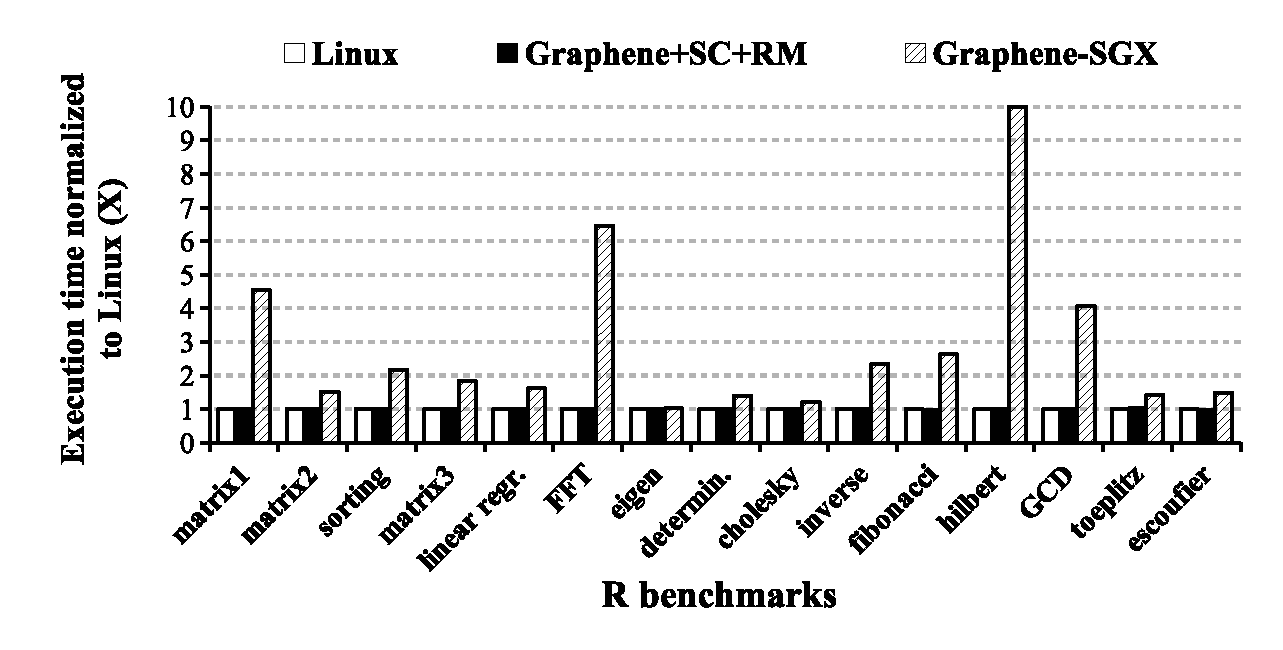
\includegraphics[width=\linewidth]{sgx/r-overhead}\\
{\bf (a) R}
\end{minipage}
\begin{minipage}{.275\textwidth}
\centering
\includegraphics[width=\linewidth]{sgx/gcc-overhead}\\
{\bf (b) GCC}
\end{minipage}
\begin{minipage}{.25\textwidth}
\centering
\includegraphics[width=\linewidth]{sgx/curl-overhead}\\
{\bf (c) CURL}
\end{minipage}

\caption{Performance overhead on desktop applications, including latency of R, execution time of GCC compilation, download time with CURL. The evaluation compares native Linux, \graphene{}, and \graphenesgx{}.} %{\bf Enclave creation time is deducted from the GCC execution time.}}
\label{fig:desktop-overhead}
\end{figure*}



\subsection{Command-Line applications}


We also evaluate the performance of a few commonly-used command-line applications.
%, to evaluate the performance of \graphenesgx{} on PCs instead of servers and clouds.
Three off-the-shelf applications are tested in our experiments:
{\bf R} (v3.2.3) for statistical computing~\cite{r-project}; {\bf GCC} (v5.4), the general GNU C compiler~\cite{gcc}; {\bf CURL} (v7.74), the default command-line web client on UNIX~\cite{curl}.
These applications are chosen because they are frequently used by Linux users,
and each of them potentially  be used 
in an enclave to handle sensitive data---either on a server or a client
machine.
% can realize profitable scenarios of using enclaves on desktop machines.



We evaluate the latency or execution time of these applications. 
%, because desktop users tend to care more about responsiveness than throughput.
In our experiments, both R and CURL have internal timing features to measure the wall time
of individual operations or executions.
%However, for other applications like GCC which does not include internal timing, evaluating the execution time can be influenced by many factors.
On a Linux host, the time to start a library OS is higher than a simple 
process, but significantly lower than booting a guest OS in a VM or
starting a container. 
Prior work measured Graphene (non-SGX) start time at 641 $\mu$s~\cite{tsai14graphene}, whereas starting an empty Linux VM takes 10.3s and starting a Linux (LXC) container takes 200 ms~\cite{agarwal15container}. 
%% dp; Note that this is MILLI seconds, not micro seconds.
%average memory footprint of an empty Linux VM, with memory deduplication, is about 96MB, . 


On SGX, the enclave creation time is relatively higher, \fixme{added more detailed number} ranging from 0.5s (a 256MB enclave) to 5s (a 2G enclave), which is a fixed cost that any application framework
will have to pay to run on SGX.
%For library OSes, the time for creating and initializing an enclave is not trivial, because it is similar to booting an lightweight OS.
% a significant part of the start-up time
% of an application is more significant, because creating enclaves is expensive.
%We consider the enclave creation time as a fixed cost for any application running in \graphenesgx{},
%and acceptable to users as long as it is responsive.
Enclave creation time is determined by the latency of the hardware and the Intel kernel driver, and is primarily a function of the size of 
the enclave, which is specified at creation time because it affects the enclave signature. %\fixmedp{although can't it grow with eadd?}.  
For non-server workloads that create multiple processes during execution,
such as GCC in Figure~\ref{fig:desktop-overhead},
the enclave creation contributes a significant portion to the execution time overheads, illustrated as a stacked bar.
%Since the enclave creation time is related to the enclave size, and unrelated to the workload,
%we deduct the enclave creation time from the execution time of GCC in Figure~\ref{fig:desktop-overhead}. \fixmedp{I think it might be better to show this as a stacked bar instead of just removing it.  Opaquely subtracting this cost doesn't seem right.  Let's discuss dp: I thought we agreed to change this...}

{\bf R}~\cite{r-project} is a scripting language often used for
data processing and statistical computation.
With enclaves, users can process sensitive data on an
OS they don't trust.
We use an R benchmark suite developed by Urbanek et al.~\cite{r-benchmark-25}, which includes 15 CPU-bound workloads such as matrix computation and number processing.
\graphenesgx{} slows down by less than 100\% on the majority of the workloads, excepts the ones which involve allocation and garbage collection: ({\tt matrix1} creates and destroys matrices, and both {\tt FFT} and {\tt hilbert} involve heavy garbage collection.)
Aside from garbage collection, these R benchmarks do not frequently interact with the host.
We further note that non-SGX \graphene{} is as efficient as Linux on all workloads, 
and these overheads appear to be SGX-specific.
%\fixmedp{Check this pontification}
In our experience, garbage collection and memory management code in managed language runtime
systems tends to be written with assumptions that do not match enclaves,
such as a large, sparse address space or that memory can be demand paged 
nearly for free (SGX version 1 requires all memory to be mapped
at creation); a useful area for future work would be to design
garbage collection strategies that are optimized for enclaves.
%we believe the overheads on \graphenesgx{} are contributed by enclaves.
 
{\bf GCC}~\cite{gcc} is a widely-used C compiler.
By supporting GCC in enclaves, developers can compile closed-source applications on customers' machines,
without leaking the source code.
GCC composes of multiple binaries, including {\tt cc1} (compiler), {\tt as} (assembler), and {\tt ld} (linker).
Therefore, GCC is a multi-process program using \syscall{execve}.
We test the compilation of thee source files with varied sizes,
using single C source files collected by MIT~\cite{gcc-benchmark}.
Each GCC execution typically \fixme{it's five, not four} creates five processes, and we run each process in a 256MB enclave by default.
%and has a fixed cost on enclave creation, which is unrelated to workload and depends on the enclave size.
%\fixme{check this}
\fixme{clarified this part, to prevent confusion between latency and overhead. also, GCC numbers got better.}
For a small workload like compiling {\tt gzip.c} (5 kLoC), running in \graphenesgx{} (4.1s) is 18.7$\times$ slower than Linux (0.2s).
The bulk of this time is spent in enclave creation, taking 3.0s in total, while the whole execution inside the enclaves, including initialization of the library OS and OS shield, takes only 1.1s, or 4.2$\times$ overhead.
For larger workloads like {\tt oggenc.c} (50 kLoC) and {\tt gcc.c} (500 kLoC), 
the overhead of \graphenesgx{} is less significant. % (3.6$\times$ and 2.1$\times$ overhead, respectively).
For {\tt gcc.c} (500 kLoC), we have to enlarge one of the enclaves ({\tt cc1}) to 2GB,
but running on \graphenesgx{} (53.1s) is only 2.1$\times$ slower than Linux (17.2s),
and 7.1s is spent on enclave creation.
%and the creation of four enclaves takes 8s.
%Each compilation has a fixed enclave creation time in \graphenesgx{}, which is about 1--2 seconds per enclave. We deduct the creation time of all enclaves  to gain more meaningful results, but do not hide rest of the overhead on fork.
%\fixmedp{Also not comfortable with this; add a bar?}
%In general, GCC in \graphenesgx{} is 1--5$\times$ slower than GCC on native Linux. 
%\fixmedp{This really needs some profiling if possible}
The overhead of non-SGX \graphene{} on GCC is marginal.
 



{\bf CURL}~\cite{curl} is a command-line  web downloader.
\graphenesgx{} can make CURL into a secure downloader that attests both server and client ends.
We evaluate the total time to download a large file, ranging from 1MB to 1GB, from another machine running Apache. % over Gigabit LAN.
%across high-speed university network\fixmedp{more specific, as above}.
\graphene{} has marginal overhead on CURL, and
\graphenesgx{} adds 7--61\% overhead to the downloading time of CURL, due to the latency of I/O.


\begin{figure*}[t!]
\centering

\begin{minipage}{.3\textwidth}
\centering
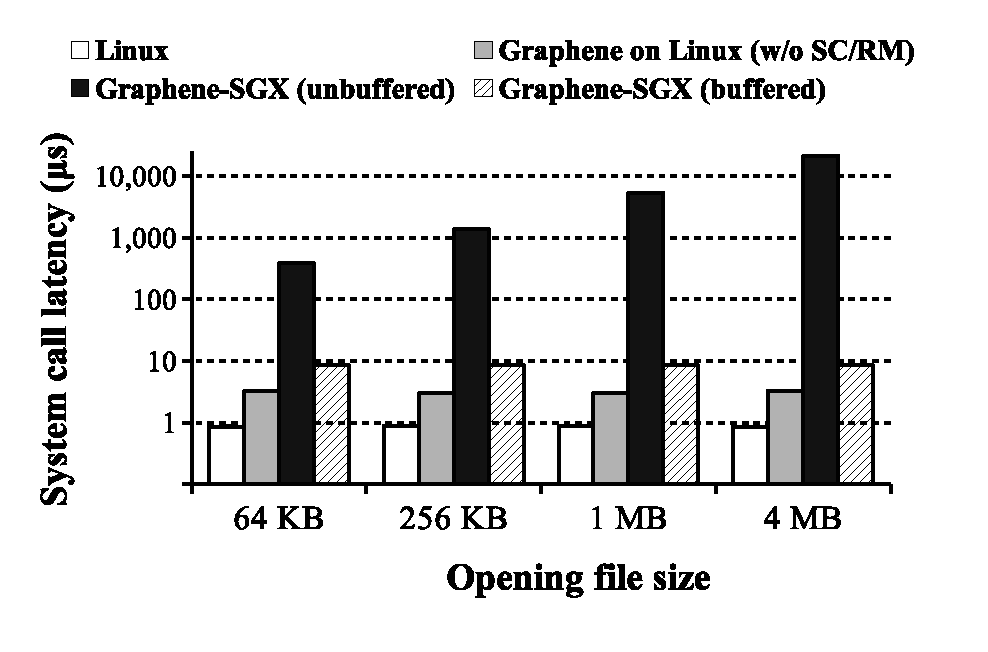
\includegraphics[width=\linewidth]{sgx/open-latency}\\
{\bf (a) Open a file}
\end{minipage}
\begin{minipage}{.3\textwidth}
\centering
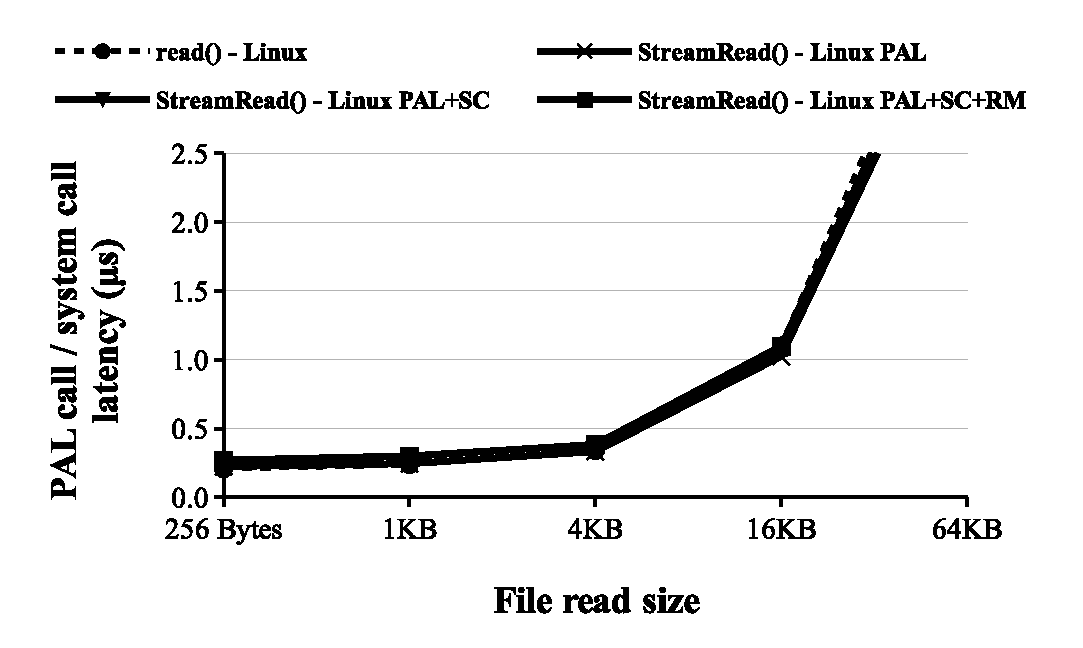
\includegraphics[width=\linewidth]{sgx/read-latency}\\
{\bf (b) Read a file}
\end{minipage}
\begin{minipage}{.3\textwidth}
\centering
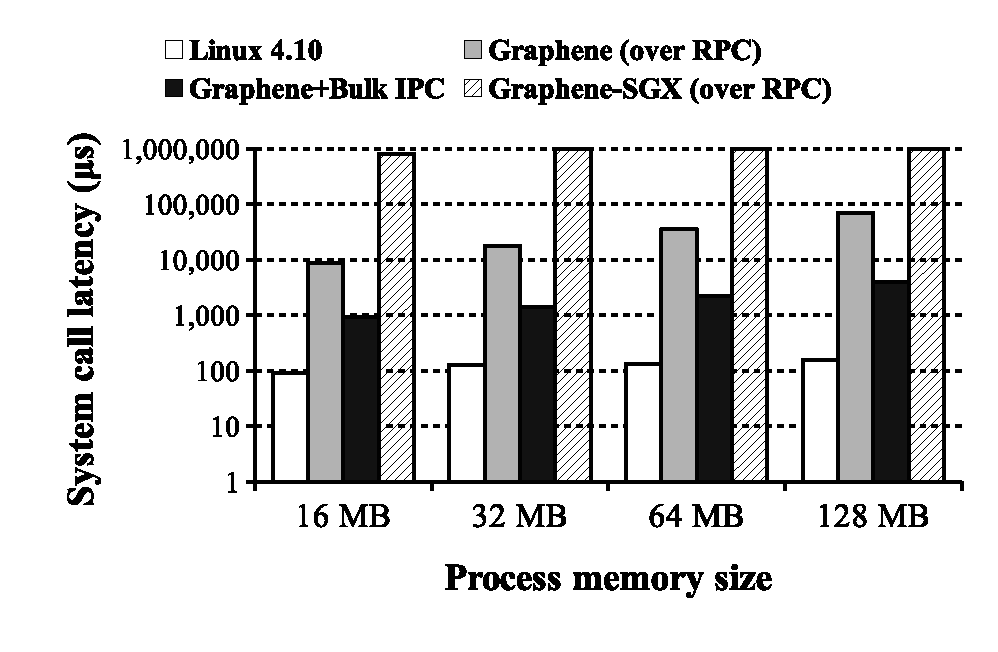
\includegraphics[width=\linewidth]{sgx/fork-latency}\\
{\bf (c) Fork a process}
\end{minipage}

\caption{Latency of some expensive system calls in \graphenesgx{}, including opening and reading a secured (authenticated) file, and forking a new process. The results are compared with native Linux and \graphene{}.}
\label{fig:syscall}
\end{figure*}


\subsection{Performance Overhead Analysis}


In this section we evaluate a few system operations that are heavily impacted by the \graphenesgx{} design.
%To shield dynamic loading and process creation,
%\graphenesgx{} uses computationally-expensive cryptographic techniques \fixmedp{more specific?} to verify enclave inputs.
% under the circumstance that the host OS cannot be trusted.
%As a trade-off to the security, the performance will be affected
%by additional cryptographic computation.
We measure the \syscall{open}, \syscall{read}, and \syscall{fork} system calls
using LMbench 2.5~\cite{McVoy:lmbench}.
A primary source of the overheads on these system calls is the cost of shielding applications, with run-time checks on the inputs.
Cryptographic techniques are used to: (1) validate the file against the secure hash, at \syscall{open}, (2) check the file chunks against the Merkle tree, at \syscall{read}, and (3) establish a TLS connection over inter-enclave RPC, at \syscall{fork}.
%opening a integrity-sensitive file for the first time, 
% or using cryptographic techniques, such as secure hashing, to verify the inputs.
% microbenchmarking specific system calls: 
% system calls,
%with different application settings.
%The microbenchmark is part of the LMBench 2.5 test suite
%\fixmedp{maybe merge this in the above paragraph, which feels a little coy}
%For instance, in order to shield dynamic loading, \graphenesgx{} checks each binary file against the secure hashes in the manifest,
%when the file is opened for the first time---after the whole file is copied into the enclave.
%\fixmedp{This happens after they are copied into enclave, memory right?}
%The verification happens when opening the file for the first time (often by the 
%After \graphenesgx{} validates the file, we generate a series of hashes of the file in chunks, as a merkle tree.
%to prevent verifying the whole file again when later randomly reading a part of the file.
%\fixmedp{So is this for the case when a file is swapped out?  I'm confused here - some details are missing}
%The latency of opening and reading an authenticated file in \graphenesgx{} is dominated by SHA256 and SHA512 calculation.
The remaining overheads contribute to exiting the enclave for host system calls, and bringing memory into the EPC (enclave page cache) or decrypting 
memory on a last-level cache miss. %and later the cache where the memory is decrypted by the CPU.


Figure~\ref{fig:syscall}(a)
shows the overhead for authenticating files in \syscall{open}.
\fixme{change overhead to latency}
Depending on the file size, the latency of \syscall{open} on \graphenesgx{} is 383$\mu$s (64KB file) to 21ms (4MB file), whereas on Linux, the latency is constant at 0.85$\mu$s.
We note that this is where enclaves are at a disadvantage, as \syscall{open} 
normally does not need to read file content; whereas here \graphenesgx{} uses \syscall{open}
as a point at which to validate file content.
For a subsequent \syscall{open}, when the Merkle tree is already generated, the overhead of simply exiting enclave for \syscall{open}, and searching the file list in the manifest, is about 9$\times$.
%\fixmedp{why?}


One might be able to optimize further for cases where only part of a file is accessed
with incremental hashing.  However, in the common case where nearly all of the file is accessed,
these costs are difficult to avoid when host file system is untrusted.
Another opportunity 
is to create the Merkle tree offline, when the manifest is created.
%\fixmedp{I think the second idea has legs...}


%This is an inevitable cost, because normal \funcname{open} on trusted OSes
%need not to access file content.
%After verifying the file, \graphenesgx{} buffers the chunk hash values, to skip whole-file verification when the file is reopened.

Figure~\ref{fig:syscall}(b)
shows the overhead for authenticating files in \syscall{read}, which 
is lower than \syscall{open}.
Since the whole file has been verified at \syscall{open}, the sequential \syscall{read} only verifies the chunks of files it is reading from untrusted memory.
%Reads from data cached in enclave memory are cheaper.  %\fixmedp{right? can we say how much cheaper?  Maybe add separate bars for both cases?}
% Therefore, \syscall{read} is actually much cheaper than \syscall{open}.
Depending on the size of blocks being read, the latency on \graphenesgx{} is 0.5$\mu$s (64-byte \syscall{read}) to 16.9$\mu$s (4KB \syscall{read}). The latency of \syscall{read} on Linux is \roughly{}0.1$\mu$s for any block size below 4KB.
If the file is not authenticated,
\graphenesgx{} only copies the file contents into the buffer, and the overhead reduces to 48\% (64-byte \syscall{read}) to 83\% (4KB \syscall{read}).
\fixmedp{Consider doing larger buffers, say up to 64k or even 4 MB}

%\fixmedp{In the legend for 7b, unsecure should be insecure}


Figure~\ref{fig:syscall}(c) shows the overhead of forking a process.
As described in \ref{sec:multiproc}, the latency of \syscall{fork} in \graphenesgx{} is affected by three factors:
creation of a new enclave, local attestation of the integrity, and duplicating the process state over an encrypted RPC stream.
Combining these factors, \syscall{fork} is one of the most expensive calls in \graphenesgx{}.
%, but at least it is supported natively on the current hardware.
The default enclave size is 256MB.
%which takes \roughly{}0.5s to create. 
Our evaluation shows that the latency of forking a process is around 0.8s (16MB process) to 2.7s (128MB process), but can be more expensive if the parent process uses more memory.
The trend matches the performance of \graphene{} without the bulk IPC optimization.
\fixmedp{If you want, some thoughts on how this might be improved in the future would be nice...  One good suggestion is recycling enclaves, or pre-forking so measurements can be done in parallel}
%Due to the overhead on \funcname{fork}, \graphenesgx{} is not suitable for fork-intensive workloads like Bash scripts
%if performance is critical.

\fixme{talk about a limitation of improving fork. check this.}
One way to further optimize \syscall{fork} is to reduce or avoid enclave creation time; one can potentially pre-launch a child enclave, and then migrate the process contents later when \syscall{fork} is called.
There might be another opportunity to improve the latency of process migration,
if copy-on-write sharing of enclave pages can be supported in future generations of SGX.
%Unfortunately, sending the process contents is difficult to avoid in \syscall{fork},
%as SGX disallows sharing enclave memory between multiple enclaves.

%\fixmedp{I assume 5.4 isn't done yet}



\subsection{TCB Size and Shielded Functionality}

In this section we measure the increase in TCB size of \graphenesgx{},
%in lines of code, 
as well as 
%compare the TCB size increased by \graphenesgx{} to an unmodified application, in lines of code, and 
the OS functionality shielded by the framework.
We compare to \scone{} and \panoply{}, using
%For SCONE and Panoply, we use 
numbers reported in their papers. 
%The conventional One generally assumes 
A smaller TCB is generally easier to review or possibly verify,
and is assumed to have fewer vulnerabilities.
%more implies lower burden for code review or formal verification, and less risk of writing exploitable code.
%For instance, Panoply argues that, because its use cases are typically smaller than 20kLoC, including both the application logic and Panoply itself, it is within the realm of future, automated verification~\cite{shinde17panoply}.

\fixmedp{Reviewer B asks for memory footprint, which isn't a bad idea}

\begin{table}
\footnotesize
\centering
\bgroup
\def\arraystretch{1.2}
\setlength{\tabcolsep}{0.5em}
\begin{tabular}{>{\raggedright\arraybackslash}p{9em}>{\raggedleft\arraybackslash\bf}p{7em}>{\raggedleft\arraybackslash}p{4.25em}>{\raggedleft\arraybackslash}p{4.25em}}
Components                    & \graphenesgx{}  & \scone{}     & \panoply{}  \\
\hline
libc (ld, libm, pthread)      &  1,292 &   88 & --      \\
                              & (glibc-2.19) & (musl)   &          \\
Library OS                    &     34 &  --      & --     \\
PAL / OS Shield               &     22 &   99 & 10  \\
\hline
Total                         &  1,348 &  187 & 10  \\
\hline
\end{tabular}
\egroup
\caption{TCB size (in thousands of lines of code) of \graphenesgx{}, \scone{}, and \panoply{}.}
\label{tab:tcb-size}
\end{table}

Table~\ref{tab:tcb-size} lists the lines of code in each components within the TCB of \graphenesgx{}, \scone{}, and \panoply{}.
By comparing the total TCB size, \graphenesgx{} is 9$\times{}$ larger than \scone{}, and 134$\times{}$ larger than \panoply{}.
However, the primary difference is the selection of libc: 
for maximum compatibility, \graphene{} uses glibc.
\scone{} uses the smaller musl libc, which lacks some features of glibc.
%it would be easy to use the smaller, and incomplete, musl libc.
%SCONE uses 
% Linux applications, \graphenesgx{} chooses to use a minimally-modified glibc, whereas SCONE uses the much more lightweight musl and 
\panoply{} excludes libc from its TCB,
% \fixmedp{what is their rationale, again? Check this}
to fit into the range of automated formal verification,
as they shield at the libc interface.
In principle, \graphene{} could easily support musl as well as glibc for applications
that do not need the additional features of glibc.
We also see the benefit of removing unused code from 
libraries, especially in an unsafe language,
similar to the approach taken in unikernels~\cite{unikernels}.
On balance, 
this choice of libc implementation is largely orthogonal to the issue
of how general-purpose the shields are.

%We argue that the choice of libc is orthogonal to the design of \graphenesgx{}; one can statically compile the applications against musl or glibc if TCB size is a concern, or given plenty of time, trim the libc functionality to bare minimum. 

If we focus on the TCB size of the library OS and the shields, 
\graphenesgx{} is 
%library OS and PAL in \graphenesgx{}, with the shielding layer of SCONE, we are 
44\% smaller than \scone{}. 
We cannot analyze the size of \scone{} because it is closed source.
%, although
%we suspect
%Although it is unclear what is in the implementation of SCONE, because it is not yet open-sourced, we believe the largest portion of their TCB contributes to the cryptography library.
\panoply{} has a smaller TCB in its shield, but within the same order of magnitude.
Panoply only shields 91 out of 256 supported POSIX functions; for context, POSIX 1003.1 defines 1,191 APIs~\cite{POSIX1003-1-2008}.
%out of 256 currently supported by \panoply{} \fixmedp{The better number is how many total functions in POSIX}.

All three of these compatibility layers or shields are within the same
order of magnitude in code size, and the differences are likely 
correlated with different ranges of supported functionality.
A recent study indicates that only order-of-magnitude differences in code
size correlate with reported CVE vulnerabilities; within the same order-of-magnitude,
the data is inconclusive that there is a meaningful difference in risk~\cite{security-metric}.
Thus, increased generality does not necessarily come with 
increased risk. % is not a clear relationship between risk 

% data only correlates
%with differences in code size when 

%Besides the choice of libc, we argue that the TCB size of a library OS or a shim shielding layer is actually correlated with the functionality that it supports or shields. Because none of the three frameworks have completely shielded the whole Linux system call table or POSIX, it is unclear how much code has to be added in the future. \graphenesgx{} also shows that one can always engineer a library OS with a small TCB, if most code is not reused from a monolithic OS kernel like Windows or Linux.
%A recent study of the CVE database also points out that having a larger TCB does not necessarily indicate more vulnerabilities, even when the difference is more than two order-of-magnitude. 



\input{apistudy}

\makeatletter
\def\input@path{{}}
\makeatother
\graphicspath{{}}
\section{Summary}



The Linux PAL successfully leverages a limited subset of Linux system calls,
to implement the whole PAL ABI for running a
full-featured \libos{}.
\Thehostabi{} separates the development of a host OS or hypervisor
from the complexity of emulating a sufficiently-compatible
Linux kernel.
The chapter shows that most calls in \thehostabi{}
can be directly translated to similar system calls on a Linux host kernel.
Only a few \hostapis{}, such as process creation and inter-thread synchronization, require additional attention for developing an efficient implementation strategy.



The Linux PAL also enforces robust security isolation
between mutually-untrusting applications,
by placing applications in separate, VM-like sandboxes.
The security isolation on a Linux host is based on system call restriction using a \seccomp{} filter, and a trusted reference monitor. % for checking resource access.
Security isolation at the host interface
restricts an untrusted application to explore vulnerable execution paths
inside a Linux kernel.
A \seccomp{} filter 
enforce a fixed, minimal system call profile, regardless of bloated dependency of an application.
The reference monitor follows
simple, white-listed manifest rules listing 
all the authorized files and network addresses of an application,
using well-known semantics
such as AppArmor~\cite{apparmor} or iptable-like firewall rules~\cite{iptablesman}.
The reference monitor can further enforce dynamic, process-specific isolation by splitting a sandbox
to run a child \picoproc{} under more restricted
resource permissions.
\graphene{} on a Linux host can serve as a sandbox framework
with a reduced attack surface
upon the host kernel.








\paperchapter{Proposed Works}
\label{chap:proposal}

The thesis describes our previous contributions
to reusing legacy applications in the \graphene{} \libos{} and Linux kernels,
in consideration of security isolation and efficiency.
{\bf The completed works of the thesis are listed as follows:}
%This thesis proposes the challenges, solutions and principles,
%to mitigate limitations from innovative system designs on enabling the execution of legacy applications.
%The following list describes the contributions of the thesis,
%from a technical view:

\vspace{\baselineskip}
\begin{compactitem}

\item A Linux-compatible \libos{} called \term{\graphene{}}~\citep{tsai14graphene},
which runs legacy Linux, multi-process applications on a platform-independent host ABI.
The system delivers a distributed POSIX implementation
over simple RPC streams,
and a security isolation model to sandbox applications,
on both trusted and untrusted hosts (using \sgx{} enclaves).
We optimize
the inter-process coordination latency in \graphene{},
using a simple bulk-copy API on the host, and determining the optimal placement of OS state.
%The platforms where \graphene{} has been ported
%include Linux, FreeBSD, \osx{},
%\win{} and \sgx{} enclaves (also called \term{\graphenesgx{}}).
%\graphene{} extends the security isolation on single-process applications,
%to processes that share UNIX multi-process abstractions,
%such as forking, signaling, sharing file descriptors, \sysvipc{}, etc.
%The shared states across multiple processes of an application
%is coordinated by the distributed implementation of OS states in \graphene{},
%over the host-provided RPC streams.
%Besides an optional host abstraction ---
%bulk IPC for optimizing copy-on-write forking ---
%all multi-process abstractions are
%implemented and coordinated completely over PRC streams,
%a feature generally provided by most platforms.
%\graphene{} further supports multi-process applications in \sgx{} enclaves,
%using attestation over RPC streams
%for secure process creation.
%and isolate each \picoproc{} in individual enclave.
%When Graphene isolates multiple processes in enclaves,
%the RPC streams can be trusted using \sgx{}'s attestation feature,
%instead of relying on sandboxing by the host.
(\S\ref{chap:graphene})

\item A prototype framework called \term{Civet},
with uses guided partitioning to split the sensitive part of an legacy \java{} application into \sgx{} enclaves.
The framework overcomes several limitations of \sgx{} to allow loading \java{} classes,
including using \graphene{} to bootstrap %and secure
\java{} VM in enclaves,
interfaces for accessing in-enclave objects, % from untrusted partitions,
and exporting enclave feature APIs.
%By allow implementation of enclave in \java{},
\civet{} applies language-specific protections, % to the isolated execution,
such as information flow tracking to filter enclave output.
%that combines the isolated execution of \sgx{} and
%\java{} language protections,
%for partitioning legacy \java{} applications.
%\civet{} includes
%a tool that automates code compartmentalization,
%generating an enclave with minimal supporting \java{} classes;
%a runtime framework that loads signed classes into an enclave,
%with language protection such as information flow control at the enclave boundary;
%and \java{} APIs to seamless access the \sgx{} features such
%as attestation and secure provisioning.
%The use cases of \civet{} includes
%isolating session keys and supporting cryptography library for a SSH connection,
%%in which the  used for encrypting the connection
%%is partitioned and isolated from the rest of the application, %in the enclave,
%%protecting the generated session key while still
%%using it for encryption and decryption.
%protecting Hadoop workloads that run proprietary algorithms,
%and a web application deployed over HTTP.
\term{This work is still in progress.}
(\S\ref{chap:civet})

\item We suggest measurements for quantitatively evaluating the importances of system APIs in legacy applications,
and the completeness of legacy support in a system prototype.
The measurements are applied in a study of 
\term{Linux API usage and compatibility}~\citep{tsai16apistudy},
to draw several insights for system development.
%to provide the information missing in
%the decision-making process of system developers.
%The study uses
%a approach to measure platform compatibility as the relative completeness of prototype systems.
%Rather than considering compatibility a binary property % (``will something break?''),
%%yet for prototypes, which are necessarily in-progress,
%we use a fractional metric
%%(``how many programs will not break?'')
%which is better suited to measuring the progress of a prototype.
%Based on the study,
%we provides a range of insights into current API usage patterns.
%For instance, we identify an efficient path to implementing a new Linux compatibility layer, maximizing the additional applications per system call.
%We also identify
%that usage of many APIs is similarly distributed:
%some are widely used, and there is a sharp drop with a very long tail
%of rarely or never-used APIs.
(\S\ref{chap:syspop})

\item We design a fast path in the Linux \term{file system directory cache}
to improve the hit latency of path lookup~\citep{tsai15dcache}.
The design decouples path searching and other operations,
by caching the results of prefix checking and file attributes in kernel data structures.
%This heavily engineered OS component
%optimizes looking up paths in file systems,
%yet the searching in the directory cache is closely interleaved
%with permission checks against security models,
%and file system features such as resolving symbolic links.
%%The cause is
%%interleaving the operation of looking up cached path components
%%with implementation of specifications,
%%including permission checks against distinct security models,
%%file attribute retrieval,
%%and resolving symbolic links.
%We optimize the lookup hit latency by decoupling cache searching
%from other operations.
%%from checking permissions and attributes,
%%when the searched path is already cached (cache hit).
%%Using the locality,
%We cache the result of permission checks on path prefixes in a data structure
%called prefix check cache,
%which will be invalidated when permission changes.
%%The optimization assume hit latency is far more critical for applications
%%than renaming or permission update latency.
%The hit latency of {\tt stat} system calls on a long path
%can be optimized to up to 27\%,
%improving the execution time
%for Dovecot IMAP server by up to 12\%
%and GIT version control system by up to 25\%.
The optimization is generalized to support most Linux file system features
(e.g., pseudo-files, renaming, symbolic links, security modules).
(\S\ref{chap:dcache})


\end{compactitem}


\vspace{\baselineskip}
\noindent
For the fulfillment of this thesis, we proposed several research and engineering
targets, and a concrete schedule for the completion of the proposed works. {\bf The proposed works and schedule are listed as follows:}


%\papersection{Proposed Schedule}
%
%The following list describes the goals and expected timelines,
%for the fulfillment of doctoral dissertation:
%


%\item \underline{\bf Publication goals:}
%
%\begin{compactenum}[A.]
%
%\item \label{enum:asplos17}
%{\bf August 15th:}\\
%\asplos{} 2017.
%Topic: Combining Hardware and Language Protections for Partitioned Applications
%
%\item \label{enum:tocs-graphene}
%{\bf Late-September:}\\
%\tocs{}.
%Topic: Cooperation and Security Isolation of Library OSes for Multi-Process Applications (Journal version). 
%
%\item \label{enum:eurosys17}
%{\bf October 21st:}\\
%\eurosys{} 2017.
%Topic: Splitting Multi-Process Applications in Multi-Enclave Library OSes
%
%\item\label{enum:sosp17}
%{\bf Mid-April:}\\
%\sosp{} 2017.
%Topic: Realizing Security Models on Secure Platforms
%
%
%\end{compactenum}


\begin{itemize}

\item \underline{\bf Schedule for Fall 2016 Semester:}

\begin{compactitem}

\item {\bf September:}\\
{\bf Collect and apply the feedbacks from the committee.}
A updated thesis proposal shall be submitted to the committee at the end of September,
including the new issues and topics
suggested by the committee.
For each suggested topics from the committee,
present
related studies, literatures, challenges and preliminary solutions.
%Simultaneously, prepare for publication goal~\ref{enum:tocs-graphene}.
\vspace{0.5\baselineskip}

\item {\bf October:}\\
{\bf Complete and improve the result of partitioning \java{} applications (\S\ref{sec:future:partitioning}).}
Complete the \civet{} framework
and support the partitioning of all the proposed use cases (SSH clients, Hadoop algorithm, and secure data manager).
Design a more efficient class Shredder, by removing unused methods from all supporting classes.
Reduce the binary size loaded into the enclave, including the \java{} VM, the \graphene{} \libos{}, libc, and JNI libraries. 
%Deliver reasonable and significant improvement on
%partitioning
%\java{} applications an
%reducing the TCB in \graphene{} \libos{} (as described in \S\ref{sec:future:partitioning}).
%Simultaneously, prepare for publication goal~\ref{enum:eurosys17}.
\vspace{0.5\baselineskip}

\item {\bf November:}\\
{\bf Implement missing features in the \graphene{} \libos{} (\S\ref{sec:future:independence}).}
%Explore more generalization of the legacy support and platform independence in \graphene{} \libos{} (as described in \S\ref{sec:future:independence}).
%Design the platform-independent host abstractions
%for implementing the missing \libos{} features (Table~\ref{tab:future:abi}).
%Deliver and experiment a total port of \graphene{} \libos{} on \osx{}, \win{}, Barrelfish and L4.
Implement scheduling system calls, and hardware support features such as hugepages and NUMA control. Introducing file system drivers, for mounting and coordinating
Networked File System (NFS) and Ext4 file system. Improve and evaluate the completeness of \graphene{} using the measurement and approach described in \S\ref{chap:syspop}.
\vspace{0.5\baselineskip}

\item {\bf December:}\\
{\bf Porting the \graphene{} host ABI to \win{}, \osx{}, Barrelfish and L4 (\S\ref{sec:future:independence}).}
Complete and evaluate the partial implementation of the \graphene{} host ABI on \win{} and \osx{}.
For the \win{} port of \graphene{}, remove the dependency on toolchains (i.e., {\tt CygWin}).
Implementing the host ABI on Barrelfish, with porting the \graphene{} \libos{} to x86 (32-bit) and ARM architecture.
Implementing the host ABI using the L4 \microkernel{}.
\vspace{0.5\baselineskip}


\end{compactitem}

\item \underline{\bf Schedule for Spring 2017 Semester:}

\begin{compactitem}

\item {\bf January:}\\
{\bf Explore the solutions for implementing security models in \graphene{} (\S\ref{sec:future:security}).}
Present use cases
for demonstrating the practicality of emulating security models in \liboses{}.
Based on the proposed designs, analyze the potential threats in the emulation models.
Deliver preliminary result of emulating security models in \graphene{}
(in both \picoprocs{} and enclaves).
Demonstrate proof-of-concepts for the implementation and prevention of vulnerabilities.
Consider research contributions and determine a publication plan.
\vspace{0.5\baselineskip}

\item {\bf February:}\\
{\bf Complete the thesis draft.}
The completed draft must include the updated content since the thesis proposal.
Describe new finding, achievements and research contributions.
The first draft will be iterated with the adviser
and polished.
The completed draft must be submitted to the Committee by the end of February,
for collecting feedbacks.
\vspace{0.5\baselineskip}

\item {\bf March:}
{\bf Collect feedbacks from the Committee and prepare for the thesis defense.}
%Collect and apply feedbacks based on the suggestions
%of the committee.
%Continue polishing the dissertation draft
%and prepare for the dissertation defense.

\item {\bf Mid-April:}
{\bf Doctoral dissertation defense and submit the thesis.}

\end{compactitem}

\end{itemize}

%In our previous works, we explore several models of enabling
%whole or part of legacy applications
%in different system designs and platforms
%(i.e., \liboses{}, \sgx{} enclaves, optimized directory cache).
%%reusing or resurrecting the development efforts in legacy code
%%that occur in diverse scenarios.
%%The cases studied include
%%partitioned systems such as library OSes,
%%conventional components in legacy OSes such as file system directory cache in Linux,
%%and partitioning a legacy \java{} application for isolated execution.
%For future works and the fulfillment of the thesis,
%we will explore
%opportunities in generalizing the current works to more use cases,
%and mitigating the principal weaknesses.

%improving the solutions in more generalized models,
%and reducing the weaknesses we observe in these solutions.
%that occur in diverse scenarios.
%For instance, \graphene{} and \gsgx{} both utilize a highly compatible library OS,
%but isolate applications with drastically different assumptions.
%In addition, \gsgx{} and \civet{} relies on two distinct strategies to maximize the usability
%--- \gsgx{} secures an application as it is, whereas \civet{} benefits from language techniques.
%As future works, we will focus on improving \graphene{}, \graphenesgx{} and \civet{},
%to build more generalized models, and minimize the weakness we have observed in these solutions.


In the following sections, we will discuss the motivations and observations
driving the proposed works.
Potential, reasonable solutions or strategies
to complete the proposed works
will be described in length, with the discussion of the related issues and principles.


\papersection{Generalizing Platform Independence}
\label{sec:future:independence}

Existing \liboses{} support legacy applications
by implementing the OS abstractions and personalities,
%that the applications depend on,
using the interfaces provided on the host platforms.
The responsibility of \liboses{} % in the process
is essentially translating the abstractions or APIs to the host interfaces and conventions.
In addition,
to provide \term{platform independence},
\liboses{} rely on the definition of host ABI to be
generic enough for the underlying platforms~\citep{porter11drawbridge, baumann13bascule, baumann14haven, tsai14graphene}
--- assuming that porting the host ABI to new platforms
will be reasonably easy.
%the semantics and assumptions of the ABI are supposed to be
%reasonably feasible for implementation
%on most host platforms.
The abstractions in the host ABI
include the commonly shared features of most platforms,
such as file systems, networks, memory mappings, etc,
with the semantics defined as translatable as possible.
%For instance, most platforms provide the abstractions and features
%of a hierarchical file system,
%with operations for opening,
%accessing and querying the files,
%using similar interfaces.
%Whether the host ABI can be ported to most platforms
%and provide host features for high-level APIs that the \liboses{} cannot internally implement,
%is the key to generalizing the platform independence.
The key to the platform independence is the portability of the host ABI,
as well as its completeness to support \liboses{} for implementing all high-level system APIs.



%Platform independence in library OSes are demonstrated by the complexity of legacy applications being supported,
%on top of various host platforms.
%The rationale behind the argument of such a proof-of-the-concept is that
%a complex application will exercise a wide range of system features and conventions,
%that mostly overlap with the common footprints of other applications.
%For instance, Drawbridge~\cite{porter11drawbridge} is tested with
%popular \win{} applications such as Internet Explorer and Microsoft Powerpoint.
%To demonstrate the platform independence of the host ABI,
%\graphene{} is ported to many platform such as FreeBSD, \win{}, \osx{} and \intel{} \sgx{} enclaves,
%and most applications can be supported on all these platforms
%transparently.

The narrowness of host interfaces causes limitations for \liboses{} to implementing OS personalities.
In existing \liboses{},
the host ABI is mostly defined for supporting \liboses{} with single OS personality:
%The primary reason is that the definition of host interfaces
%is mostly biased by the specifications that developers choose to implement,
%and the applications preferred for testing.
For instance, in \drawbridge{}~\citep{porter11drawbridge}, the host ABI
is defined to support a \libos{} with \win{} personality.
%, which is adopted by many other library OSes,
%is defined for a library OS of \win{} personality.
In \graphene{}, we implement Linux personality over the \drawbridge{} host ABI,
and observe a few necessary, but missing host abstractions,
due to the difference between the platforms.
A similar process is taken by another \libos{}, Bascule, that inherits the \drawbridge{} host ABI.
For instance, Linux applications heavily rely on exception handling,
but the relative host interface to set up handlers
is missing in \drawbridge{}, and added in both Bascule and \graphene{} afterward.

In this thesis we focus on implement Linux personality:
\graphene{} supports \syscalls{} Linux system calls,
selected by what we considered to be the most commonly used.
However, according to our study of Linux system API usage in a large, representative application sample,
for any Linux installations,
there are only 0.4\% of the installed applications whose system API footprint
are completely supported by \graphene{}.
Moreover, the study suggests that completeness of \graphene{} can be largely boosted (from 0.4\% to 21\%)
by adding two scheduling system calls,
{\tt sched\_setscheduler} and {\tt sched\_setparam}.
In future, we will guide the implementation of system APIs
using the measurements derived from our study.


\begin{table}[t]
\footnotesize
\centering
\begin{tabular}{>{\bf}p{1.2in}>{\raggedright\arraybackslash}p{2.4in}>{\raggedright\arraybackslash}p{2.4in}}
\toprule
{\bf Host ABI Function} & {\bf Functions in the \libos{}} & {\bf Description} \\
\midrule
Scheduler policies & {\tt sched\_setscheduler}, {\tt sched\_setparam}, {\tt sched\_setaffinity} & Specifying scheduler policies such as priority level or CPU affinity in the manifests.\\
\midrule
Huge pages & {\tt MAP\_HUGETLB} flags for {\tt mmap} & Specifying virtual memory to be backed by huge pages. \\
\midrule
Memory sharing & {\tt shmget}, {\tt shmat}, {\tt shmdt} & Sharing memory using RPC. \\
\midrule
Raw sockets & {\tt socket} with {\tt SOCK\_RAW}  & Sending RAW packets (e.g., DHCP clients) \\
\midrule
NUMA & {\tt set\_mempolicy}, {\tt migrate\_page} & Accessing host NUMA features. \\
\bottomrule
\end{tabular}
\caption[List of host ABI functions to be added in \graphene{} as future works]
{List of host ABI functions that are missing in \graphene{} host ABI.
We expect supporting these functions in the future,
by either extending the host interfaces or configuration in manifest files.}
\label{tab:future:abi}
\end{table}


The Linux system calls that are not implemented in \graphene{}
% besides the one we anticipate to be supported in the near future,
can be primarily categorized into two types.
One type is the APIs
to specify policies for scheduling host resources;
and the other is to provide functionality of host hardware features.
Examples for the former type are the scheduling system calls mentioned earlier.
% such as {\tt sched\_setscheduler}.
The latter type includes
various {\tt ioctl} operations,
and \term{NUMA-related APIs} like {\tt migrate\_pages}.
These abstractions are impossible to implement in \liboses{}
without extension to the host ABI.
To complete these system calls,
we will design \term{new host interface} to expose these host abstractions
to applications,
or rely on \term{manifest file}
to specify the scheduling policy of hardware resource.
%The advance the completeness of \graphene{},
%we will design host ABI to by
%either providing an platform-independent interface
%for \picoprocs{},
%or allowing users to specify the resource multiplexing policy in the manifests.
Table~\ref{tab:future:abi} lists the first-order host abstractions
that need be provided in the \graphene{} host ABI.


\begin{table}[t]
\footnotesize
\centering
\begin{tabular}{>{\bf}p{1.2in}>{\raggedright\arraybackslash}p{0.8in}>{\raggedright\arraybackslash}p{1.6in}>{\raggedright\arraybackslash}p{2.2in}}
\toprule
{\bf Feature} & {\bf Platform} & {\bf Limitations} & {\bf Proposed strategy} \\
\midrule
Memory mappings & \win{} & No fine-grained deallocation or protection & Redesign ABI functions for platform independence \\
\midrule
Thread-local storage & \win{}, \osx{} & FS or GS register is not available & Overwrite TLS allocation in libc, or binary translation \\
\midrule
Position-dependent binaries & \win{}, \sgx{} & Memory addresses are occupied or restricted & Reserve virtual memory before \picoprocs{} start \\
\midrule
Special instructions & \sgx{} & {\tt CPUID} and {\tt RDTSC} are forbidden & Exception handling or binary translation \\
\bottomrule
\end{tabular}
\caption[List of platform limitations affecting host ABI porting]
{List of limitations on host features that affects porting the host ABI to the target platforms,
and the coping strategies.}
\label{tab:future:abi-limit}
\end{table}

%Besides the feasibility of implementing OS personalities,
We also have to demonstrate the neutrality and portability of the host ABI,
to justify that \graphene{} is independent to most host platforms.
However, the assumptions made in our host ABI definitions
can be violated on specific host platforms
due to the platform limitations and characteristics.
For instance, although not defined explicitly in the host ABI,
a Linux \picoprocs{} requires the host platforms
to reserve part of the address space (often near {\tt 0x4000000}), for loading position-dependent binaries.
% that are not compiled as position independent.
Such a requirement is a challenge to the platforms
in which the virtual memory of a process is partially preoccupied by the host,
or restricted to a specific range.
We observe the phenomenon in two of the ported platforms:
in \win{}, user stacks and PCBs (process control blocks) can overlap with the demanded address;
in \sgx{} enclaves, the range of mappable memory is
restricted to a preset region.
%processes are only allowed to access a limited range of virtual memory.
Table~\ref{tab:future:abi-limit}
lists the platform limitations that affects the implementation of host ABI,
and the proposed strategies to remove the limitations.
% for the reinforcement of platform independence.


Essentially,
justifying the platform independence of \graphene{} will
require porting its host ABI to more diverse platforms,
especially ones that do not rely on a monolithic kernel with abundant APIs.
One opportunity is to port \graphene{} to a \term{\microkernel{}}
(e.g., L4~\citep{l4family, klein09sel4}) or a \term{hypervisor} (e.g., Qemu, Xen).
Instead of relying on host features (e.g., Seccomp filter)
to restrict the attack surface of \picoprocs{},
\graphene{} ported to a \microkernel{} or hypervisor will minimize both the attack surface and the shared TCB of the host.
The functionality of \graphene{} on L4 will be similar as
L4Linux~\citep{hartig97mu},
but at a lower cost because \graphene{} does not port the whole Linux kernel to user space.
On the other hande,
a \microkernel{} or hypervisor
may provide a reduced paravirtual APIs,
without the full host abstractions required by the host ABI.
A few host abstractions that may be missing
are file access, network sockets and other single-process, multiplexed resources.
Implementing the host ABI on these platforms will requires
extension of the host paravirtual APIs, or reduction of the \graphene{} host ABI
--- for example, running an in-process file system, or a NFS (networked file system) client in \picoprocs{}.



%Porting \picoprocs{} to \microkernel{} will allow running legacy applications
%in a host with restricted resource,
%at a smaller cost than porting a whole kernel to user space

%Another platform that is worth to port \graphene{} is 
\term{Barrelfish}~\citep{baumann09barrelfish, zellweger14barrelfishdc} is a \microkernel{}-style
research OS designed for multi-core, heterogeneous environment.
Barrelfish runs applications with OS implementation tied to each heterogeneous core,
to decouple OS coordination from
architectural characteristics such as instruction sets, cache coherence, and memory hierarchies.
Not unlike \graphene{} using a
distributed, collaborative OS implementation,
Barrelfish duplicates the OS functionality
(``OS nodes'')
with independent, unshared state on each core.
Inter-core message-passing is used among OS nodes and applications
to coordinate OS state and services.
Porting \graphene{} to Barrelfish can enable the legacy support on the platform,
and extend the host architectures for \graphene{}
to include heterogeneous cores.
The implementation of \graphene{} host ABI on Barrelfish
can rely on its tool chain that partially supports the common POSIX APIs
--- including simple file IO, network sockets,
and user-space RPC.
To allow \graphene{} to run in a environment with heterogeneous ISAs,
\graphene{} will have to be ported to different architectures,
such as x86 and ARM.


We observe that many platforms provide \term{POSIX-compliant APIs},
which is the closest to a platform-independent specification.
Besides a few limitations on the \graphene{} host ABI,
such as TLS support and loading position-dependent binaries (both discussed in Table~\ref{tab:future:abi-limit}),
most of the \pal{} calls can be smoothly ported to POSIX.
A POSIX port will allow \graphene{} to be easily migrated to any POSIX-compliant platforms,
with little development effort to deal with
the rest of host ABI.





%and uses asynchronous message passing across heterogeneous cores pinned to applications.
%The distributed POSIX implementation of \graphene{}
%will be an advantage when porting it to Barrelfish.
%%In addition, the \osx{} and \win{} ports of \graphene{} are still in-progress.
%Overall, when generalizing the host ABI implementation to more platforms,
%we observe that a large portion of \graphene{} \pal{}
%can be reused for another platform.
%In particular, a wide range of platforms adopt the POSIX specifications.
%By translating the \graphene{} host ABI to standard POSIX APIs,
%the platform independence of \graphene{} can be guaranteed on
%every POSIX-compliant hosts.



\papersection{Partitioning Legacy Applications}
\label{sec:future:partitioning}


%Although \graphene{}, \gsgx{} and \civet{} can fundamentally reduce the TCB required for an application,
%we observe missed opportunities in these solutions to further minimize the risk.
%In \graphene{}, the \libos{} of untrused applications are evicted from the TCB,
%but the host kernel must still be trusted. The system call restriction enforced by Seccomp filters is helpful, but it is hard to reason that the vulnerabilities are eliminated in the kernel.
%For a system that requires stronger enforcement, the \graphene{} PAL can be ported to a bare-metal or a \microkernel{} such as L4~\citep{l4family}.
%
%In \gsgx{} and \civet{}, we observe more opportunities of reducing TCB with engineering efforts.
%For instance, \gsgx{}, the size of \libos{} and supporting libraries
%can be as large as tens to hundreds of megabytes.
%The supporting classes partitioned by the \civet{} design-time tool
%may contain more than thousands of \java{} classes.
%All these code and data are not always necessary, and can be shredded more carefully or in finer granularity.


In our ongoing work,
we explore a system design called \term{\civet{}} to automatically partition legacy \java{} applications into \sgx{} enclaves.
%to isolate a minimal, security-sensitive component
%in \intel{} \sgx{} enclaves.
%We have a prototype framework to show the proof-of-the-concept.
As a proof-of-concept,
we build a framework prototype that demonstrates the partitioning of
three representative use cases described in \S\ref{sec:civet:cases}.
For future works,
the implementation can be extended to handle more scenarios.


In particular, a primary challenge in \civet{} is
to improve the effectiveness of the partitioning
--- in other word, pursuing the minimality of the isolated, security-sensitive components.
%Another aspect of partitioning is
%the effort needed for the developers
%to identify the boundary of partitioning.
\civet{} uses a \emph{Shredder} that identifies the minimal supporting classes required
for the isolated execution,
to generate a clean, self-contained partitions
with the smallest TCB, and less resource for loading and compiling classes in enclaves.
%The fewer classes the Shredder partitions,
%the smaller code size and TCB the created enclaves have.
%Observing the effectiveness of the current Shredder,
We evaluate the effectiveness of the current Shredder design:
based on the dependency analysis from the entry classes identified by the developers,
even for a minimal ``Hello World'' enclave,
%after shredding the unused classes based on the dependency analysis from a few developer-identified interface classes,
%effectively
the Shredder generate a partition with
\~{}3,000 classes, \~{}23,000 methods,
and \~{}388,000 lines of code in total.% \fixme{Collect the actual number}.
%are still left in the partition,
%even if the component to isolate
%is simply a ``Hello World''.
Compared with the overloaded TCB of the unstripped \java{} runtime classes
(from {\tt rt.jar}),
the shredded code effectively reduces xx\% of the enclave code.
The remaining classes generated by the Shredder
includes the dependency of OpenJDK \java{} VM and the \civet{} framework,
as well as the super classes
with overridden methods that are never used.
%The resulting TCB includes
%methods used by the 
%\java{} VM class loader and the \civet{} framework;
%overridden super-class methods;
%and others that are part of a supporting classes
%but never used.
In future, we can further reduce the size of supporting classes,
by partitioning 
at the granularity of methods,
to shred all unused code in the isolated classes.


Another important aspect of partitioning is
the effort for developers
to identify the scope of partitioning,
based on the understanding of the execution.
\civet{} requires developers to provide two simple hints
for guiding the partitioning:
(1) the classes used as the enclave interfaces,
and (2) dynamically-loaded classes.
From the developers' perspective,
however,
the loaded classes are not necessarily exposed to the developers.
Due to the encapsulation and run-time loading
of \java{},
the actual loaded classes during execution
may be obfuscated to the application developers of \java{}.
%identifying these classes are not necessarily straightforward,
%as we found in our use cases.
%For example, some applications do not have the obvious interfaces
%to interact with the sensitive components,
%or, in the worst case, are not well modularized (e.g., all methods are in one main class).
%On the other hand,
A common example is the loading of \java{} cryptography APIs:
\java{} provides a generic interface
to loads encryption or other cryptographic engines
based on hard-coded or input strings that describe the algorithm options.
%\fixme{Describe details of this example.}
%sometimes the \java{} VM loads classes based on some inputs from the users or developers,
%such as loading cryptography APIs based on hard-coded or inputed strings
%which describe the algorithms and options.
%Even if developers who conduct the partitioning know the algorithms that will be used,
%it is hard to identify the actual classes that will be loaded
%unless the developers have knowledge about the internals of cryptography APIs.
To precisely analyze the loading classes
in a \java{} application,
\civet{} can rely on a training phase for detecting dynamically-triggered class loading,
or conducting sophisticated date-flow analysis
to retrieve the class names from the source or the byte-code.


An alternative approach for partitioning applications will be to determine the minimal partition ``bottom-up'',
starting from the execution or data that needs to be protected.
Instead of using a Shredder to remove unused classes,
the partitioning can instead rely on a \term{Collector} that 
starts with minimal isolated classes,
and gradually includes more byte-code into the enclave.
The Collector will
incorporate the classes
that access any protected methods or objects,
until it ultimately determines a clean,
minimal partition as self-contained and with the narrowest interface.

Besides the effectiveness for partitioning applications,
we also observe opportunities in reducing the TCB of infrastructure,
including the OpenJDK \java{} VM and its libraries,
JNI libraries,
non-\java{} code of the \civet{} framework,
and the underlying \libc{} and \graphene{} \libos{}.
In current work, we reduce the unused code on a best-efforts basis.
In future, we seek more
systematic approach
to fundamentally shrink the size of enclave code.

%the \civet{} framework, the OpenJDK \java{} VM,
%and the underlying \graphene{} \libos{},
%to further reduce the TCB.
%The unused library functions, \java{} VM features, JNI code, and system calls in \graphene{}
%can all technically be removed with manageable efforts.


\papersection{Emulating Legacy Security Models in Applications}
\label{sec:future:security}

%In \graphene{} or many others like VM or container-based solutions,
%applications are protected with a trust model of all-or-nothing.
%In other word, each process or component of an application can only be fully trusted or not trusted at all.
%The key reason of such a restriction is that the applied isolation cannot reflect the complexity of privilege model in the application.
%In reality, multiple principles can co-exist in an application.
%For instance, a web server that serves requests from clients identified as different clearance
%will need to maintain the correspondent confidentiality levels.
%The web server may perform operations that are more sensitive (e.g., retrieve a secret key)
%or more vulnerable (e.g., execute privilege-escalating scripts).
%For components in the same process, we have seen examples, such as the heart-bleed bug~\citep{heartbleed} in OpenSSL, in which sensitive components are intruded by more functional components.

In \liboses{}, security isolation is enforced on mutually untrusting applications,
to disallow OS-level interaction,
or sharing any OS and application state.
Such a model is fail-safe, but inflexible.
On the other hand, many legacy applications are already
configured with security policies,
based on existing security models adopted in commodity operating systems.
For instance, in UNIX systems, applications or processes
can be assigned with \term{credential IDs} or \term{POSIX capabilities},
to specify the privilege of accessing abstractions or resources.
In Linux, more sophisticated, fine-grained security models
such as \term{AppArmor}~\citep{apparmor} and \term{SELinux}~\citep{selinux}
can further specify the objects (i.e., \emph{``what can I access?''})
and the actions (i.e., \emph{``how can I access it?''}) of access control.
Specifically, SELinux can enforce a \term{multi-level security} model, or \term{DAC (Discretionary Access Control)},
to control the propagation of information contamination.
Both AppArmor and SELinux require configuration efforts,
and generally, the developers are responsible for
providing the profiles
that reflect the appropriate policies.
In addition,
Linux supports isolation of various \term{namespaces},
such as PID, mount points, and \sysvipc{} keys, 
to allow applications to isolate a part of the OS views in selected processes.
The isolation of namespaces is often used in the concept known as \term{containers}.
Overall, the usage of these models consists in
part of the existing development effort,
and defines the least privileges each subject requires
to fulfill its tasks, more or less.


Security models can be critical for application:
a security model can enforce policies that not only restraint unrelated applications,
but also ensure the safe behaviors of cooperating components.
In \liboses{}, applications need a model that,
when a \picoproc{} creates or interacts with others,
one can choose to put only partial trust in another.
For instance,
an Apache web server with privilege-escalating PHP scripts (e.g., suPHP)
can isolate the scope of
the script execution
with restricted policies.
When running in \graphene{},
the \picoprocs{} will coordinate OS states such as process ID namespaces or signaling,
but restrict access for specific OS abstractions. 


%due to the much larger attack surface in the PHP engine.
%However, A \picoproc{} that runs the web server
%still needs to maintains minimal coordination with the \picoproc{} running the PHP engine,
%such as connection through pipes,
%or sharing the process ID namespace for signaling.


At the center of these problems is the fact that existing \liboses{} including \graphene{}
cannot reflect \term{non-binary},
precisely-defined policies in applications.
The design of \picoprocs{} disallows any management of credentials and access control inside \liboses{},
because OS states and data structures are always
vulnerable to in-process attackers. % inside the same \picoproc{}.
In \graphene{}, every process is granted with the local \emph{root} permissions
--- allowed to access any OS resources and abstractions
in its sandbox.
Alternatively, we present a new opportunity in \graphene{},
to allow \emph{expelling} a \picoproc{} from its current sandbox (\S\ref{sec:graphene:security});
however, once a \picoproc{} is detached from a sandbox,
it is forbidden by the reference monitor to coordinate with other \picoprocs{}
by all means.


\begin{table}[t]
\footnotesize
\centering
\begin{tabular}{>{\bf}p{1.2in}>{\raggedright\arraybackslash}p{2.4in}>{\raggedright\arraybackslash}p{2.4in}}
\toprule
{\bf Security Model} & {\bf In-application example} & {\bf Proposed strategy} \\
\midrule
UID-based & Process calls {\tt seteuid()} system call for escalating or dropping privilege & Mapping UIDs/GIDs to sandboxes \\
\midrule
Namespaces & Clone child process with isolated namespaces & Isolating RPC streams and IPC helper threads for different namespaces \\
\midrule
AppArmor & Specify white-list of allowed files and network address for an application & Translating AppArmor profiles to sandbox rules \\
%\midrule
%Multi-level security &  &  \\
\bottomrule
\end{tabular}
\caption[List of security models to be added in \graphene{} as future works]
{List of security models that are missing in \graphene{}.
We expect emulating in-application policies based on different security models in the future, and propose possible strategies for emulation.}
%\fixme{Propose strategy for MLS}
\label{tab:future:security}
\end{table}

%A partitioned system that sandboxes mutually untrusting applications
%must restrict any interaction or coordination between the sandboxes.
%Take \graphene{} for instance;
%the related \picoprocs{} (created from the same application)
%in a sandbox will trust each other
%and be permitted to coordinate freely over the host RPC streams.
%On the contrary, two unrelated \picoprocs{} from separate sandboxes will be completely detached,
%with the \graphene{} reference monitor enforcing a strict,
%all-or-nothing access control on RPC streams.
%The rationale behind this design is to enforce simple but strong isolation from the host,
%instead of relying on permission checks that are fragile and subtle
%in a complex operating system.


An alternative for \picoprocs{} to enforce non-binary security
is to use the host interface
for specifying capabilities and permissions,
and rely on centralized entities---often the kernels----to mediate all 
access control.
The design is similar to the method adopted in the building blocks of \term{HiStar}~\citep{zeldovich+histar}.
In HiStar, processes are assigned with labels, which will taint the components or resources that the processes ever interact with or access,
based on the \term{information flow control} of the kernel.
Applying this model to \graphene{} will require
massive changes to the design;
all multi-process abstractions coordinated over RPC will have to be mediated by the kernel, with inevitable extension to the host interface.
Another limitation is the prerequisite of
trusting the host kernel,
which may be impractical on some platforms such as \sgx{} enclaves.

%In general, to enforce security isolation between sandboxes,
%\graphene{} must assume
%unrelated applications will never share any resources or states,
%unless completely mediated by the host.
%In other word, if two mutually untrusting applications
%will ever share a resource or state,
%\graphene{} must place the \picoprocs{} of both applications in a sandbox
%and allow any coordination among them.
%No partial isolation can be enforced in \graphene{}.
%The all-or-nothing security isolation will
%cause violation to the \emph{least privilege principle}
%if the involved parties
%require more fine-grained access control.
%In fact, partial isolation is required by many applications,
%when one process untrusts another because of the security vulnerabilities,
%still have to interact in a limited, controlled way.
%For instance,
%a web server (e.g.,Apache) may prefer to be completely detach from a PHP engine (e.g.,FastCGI-PHP),
%due to the much larger attack surface in the PHP engine.
%However, A \picoproc{} that runs the web server
%still needs to maintains minimal coordination with the \picoproc{} running the PHP engine,
%such as connection through pipes,
%or sharing the process ID namespace for signaling.
%In a sense, \graphene{} does provide dynamic sandboxing
%for \picoprocs{} that have dropped privileges,
%but the sandboxed \picoproc{} will be completely detached from the others,
%and appear to them as being destroyed.

The key to enforcing abstraction-specific policies in \liboses{}
is the placement of abstraction states
in \picoprocs{}.
In \graphene{}, each \picoproc{} can receive a state replica
from the owners of abstractions,
while the security policies are completely ignored.
However, based on the policies,
a \picoproc{} shall be permitted or rejected for
replicating the abstraction state according to whether the process is allowed to share the abstraction.
If we ensure all abstraction states to be placed in the permitted \picoprocs{},
\liboses{} can approve RPC messaging for coordination,
by either permission checks
or access control by the host.

For instance,
%A plausible model to allow partial security isolation among \picoprocs{}
%is to enforce \term{namespace} access control.
%The mechanism is similar to the namespace in UNIX system:
when a process clones a child with namespace isolation
(e.g., using {\tt CLONE\_NEWPID} flag),
the \libos{} can set up iptables-like firewall rules---a host feature
already provided by the reference monitor of \graphene{} (\S\ref{sec:graphene:security})---on the coordinating RPC streams
to restrict the access of namespace state.
The assignment of the rules on the host must happen
prior to the process creation.
%the kernel data structures related with the namespaces will be strictly separated.
%In \graphene{}, similar policies can be enforced
%by setting up firewall rules on the host RPC streams.
%Assuming a \picoproc{} strictly uses different RPC streams to coordinate different namespaces or abstractions,
%host policies can be assigned to allow another untrusted
%\picoproc{} accessing specific RPC streams.
The \libos{} will have to isolate the RPC streams and the responding IPC helper threads that manage separate namespaces.
%A even more fail-safe approach will be to assign 
%\term{BPF (Berkeley Packet Filter)} rules to filter RPC streams on the host,
%by comparing the sources or specific fields of RPC messages.

%firewall rules to filter the contents of RPC streams,
%to prevent \picoprocs{} to make mistakes on separating RPC streams.
%The \picoprocs{} can submit \term{BPF-style} (Berkeley Packet Filter) firewall rules to the reference monitors, to filter the fields in RPC messages.
%Either approaches are platform-independent, and the former one requires no changes to the current host ABI.


%Another model of non-binary security isolation
%is to enforce \term{multi-level security} (MLS) among \picoprocs{},
%so applications can be protected
%with the ``no read up, no write down'' rule.
%This model is similar to security isolation model of HiStar~\citep{zeldovich+histar}.
%The \liboses{} will enforce DAC-type (Discretionary Access Control) policies,
%by labeling \picoprocs{} based on the level of secrecy or integrity.
%Among the \picoprocs{}, \term{information flow} can be implied to
%determine whether a \picoproc{} is allowed to send or receive RPC messages
%on the host streams connected with other \picoprocs{}.
%The directional access control on host RPC streams is
%a reasonable extension to the host ABI.




We propose strategies for emulating different security models in \liboses{}  (discussed in table~\ref{tab:future:security}).
\term{Credential IDs}, such as user IDs or group IDs,
are commonly used to specify the owner of objects in operating systems,
primarily for
isolating users that share the same  host.
In other use cases, however, credentials can matter even in a single application
--- when a process uses system calls like {\tt seteuid()} and {\tt setegid()}
to temporarily change its privileges for accessing resources.
We can emulate credential IDs by mapping the credentials to host sandboxes.
When a process changes its credential,
the host can migrate the \picoproc{} from a sandbox to another,
as long as the migration
does not compromise either of them.
Another common security model used in Linux, \term{AppArmor}, 
allows developers to specify a profile for an application,
to white-list
all the files, network addresses, and other resources
permitted in the application.
In fact, the policies specified in AppArmor are conceptually similar
to sandboxing in \graphene{}.
We can simply emulate AppArmor model in \graphene{} by translating the AppArmor profiles into sandbox rules.
%\fixme{Rethink about MLS and SELinux}

Speaking at the high level,
emulating security models in a platform-independent way
is fundamentally a research problem. 
From the perspective of developers and users,
they choose security models---among the available options of their preferred systems---based on what they see suitable for
the applications.
The secure platforms (e.g., \liboses{}, \microkernel{}, \sgx{} enclaves), on the other hand,
determine the architectures and mechanisms for
enforcing certain security principles.
As a future direction,
decoupling security models (\emph{``what to secure?''}) and secure platforms (\emph{``how to secure?''})
will provide more options
for developers and users to define their desired policies.




%\papersection{Seamless Transition of Partitioned Systems}




%\papersection{Future Directions}

%
%\paragraph{Security Isolation for Multi-Principle Applications.}

%
%\paragraph{Seamless Transition of Security Isolation.}
%Each existing solution of security isolation can protect applications
%under specific security principles and assumptions.
%For instance, \graphene{} or other \picoproc{}-based solutions isolate mutually untrusting applications on a trusted host,
%whereas enclaves protect more sensitive applications on an untrusted host.
%No existing solutions can support all security principles and assumptions.
%Moreover, many solutions provide a container-like environment in which the operating system views are completely isolated.
%These limitations cause different solutions to be mutually exclusive,
%and users are held responsible for making the decisions of choosing the solution
%--- simply put, to explicitly run {\tt pal} or {\tt pal-sgx} to load applications in \graphene{} or \gsgx{}. 
%The penalties of the security solution such as performance overhead or incompatibility
%will make users to be reluctant
%to choose one solution to run all related applications,
%if given the choice.
%
%%Security isolation for applications mostly requires users to run applications in a container-like environment, consciously and explicitly.
%%Simply put, a user must always launch an application in \graphene{} or \gsgx{} by executing their loaders, {\tt pal} or {\tt pal-sgx}.
%%In practice, however, users often have insufficient knowledge of the requirement of applications
%%to decide whether to enforce stronger security isolation.
%%The common result of the problem is that isolation solutions becomes mutually exclusive for an operating system to choose.
%
%While operating systems have sufficient information to determine the security principles of an application,
%the existing solutions of security isolation
%are not designed to seamlessly transit into one another.
%We can use \graphene{}, \gsgx{} and Linux as an example of transition between solutions.
%%We observe that \graphene{} and \gsgx{} provide compatible Linux personality,
%%so that applications can run seamlessly in these environments.
%The Linux personality of \graphene{} and \gsgx{}
%make it feasible to dynamically migrate applications from Linux to a \picoproc{}
%%For instance, operating systems can determine how to isolate an application based on its origin
%that is signed by the developers to always run in an enclave,
%can demand a regular process to be migrated into another enclave
%if the the process is requesting any interaction
%--- a requirement that can be verified by the enclave, without trusting the Linux host.
%%while a suspicious, downloaded application will run in a \picoproc{}.
%%If a regular application interacts with the sensitive one, the latter's \libos{} can demand the former to be migrated into an enclave.
%%In contrast, if a application becomes tainted by a suspicious application,
%%operating system can migrate the application to a \picoproc{}.
%Similar technique can be applied to drop the privilege of a regular application to a \picoproc{}
%if tainted by a low-security applications already isolated in another \picoproc{}.
%
%
%\paragraph{Minimizing TCB.}




%\chapter{Proposed Works}
\label{chap:future}



In our previous works, we explore several models of enabling
whole or part of legacy applications
in different system designs and platforms
(i.e., \liboses{}, \sgx{} enclaves, optimized directory cache).
%reusing or resurrecting the development efforts in legacy code
%that occur in diverse scenarios.
%The cases studied include
%partitioned systems such as library OSes,
%conventional components in legacy OSes such as file system directory cache in Linux,
%and partitioning a legacy \java{} application for isolated execution.
For future works and the fulfillment of the thesis,
we will explore
opportunities in generalizing the current works to more use cases,
and mitigating the principal weaknesses.

%improving the solutions in more generalized models,
%and reducing the weaknesses we observe in these solutions.
%that occur in diverse scenarios.
%For instance, \graphene{} and \gsgx{} both utilize a highly compatible library OS,
%but isolate applications with drastically different assumptions.
%In addition, \gsgx{} and \civet{} relies on two distinct strategies to maximize the usability
%--- \gsgx{} secures an application as it is, whereas \civet{} benefits from language techniques.
%As future works, we will focus on improving \graphene{}, \graphenesgx{} and \civet{},
%to build more generalized models, and minimize the weakness we have observed in these solutions.



\section{Generalizing Platform Independence}
\label{sec:future:independence}

Existing \liboses{} support legacy applications
by implementing the OS abstractions and personalities,
%that the applications depend on,
using the interfaces provided on the host platforms.
The responsibility of \liboses{} % in the process
is essentially translating the abstractions or APIs to the host interfaces and conventions.
In addition,
to provide \term{platform independence},
\liboses{} rely on the definition of host ABI to be
generic enough for the underlying platforms~\citep{porter11drawbridge, baumann13bascule, baumann14haven, tsai14graphene}
--- assuming that porting the host ABI to new platforms
will be reasonably easy.
%the semantics and assumptions of the ABI are supposed to be
%reasonably feasible for implementation
%on most host platforms.
The abstractions in the host ABI
include the commonly shared features of most platforms,
such as file systems, networks, memory mappings, etc,
with the semantics defined as translatable as possible.
%For instance, most platforms provide the abstractions and features
%of a hierarchical file system,
%with operations for opening,
%accessing and querying the files,
%using similar interfaces.
%Whether the host ABI can be ported to most platforms
%and provide host features for high-level APIs that the \liboses{} cannot internally implement,
%is the key to generalizing the platform independence.
The key to the platform independence is the portability of the host ABI,
as well as its completeness to support \liboses{} for implementing all high-level system APIs.



%Platform independence in library OSes are demonstrated by the complexity of legacy applications being supported,
%on top of various host platforms.
%The rationale behind the argument of such a proof-of-the-concept is that
%a complex application will exercise a wide range of system features and conventions,
%that mostly overlap with the common footprints of other applications.
%For instance, Drawbridge~\cite{porter11drawbridge} is tested with
%popular Windows applications such as Internet Explorer and Microsoft Powerpoint.
%To demonstrate the platform independence of the host ABI,
%\graphene{} is ported to many platform such as FreeBSD, Windows, OSX and \intel{} \sgx{} enclaves,
%and most applications can be supported on all these platforms
%transparently.

The narrowness of host interfaces causes limitations for \liboses{} to implementing OS personalities.
In existing \liboses{},
the host ABI is mostly defined for supporting \liboses{} with single OS personality:
%The primary reason is that the definition of host interfaces
%is mostly biased by the specifications that developers choose to implement,
%and the applications preferred for testing.
For instance, in \drawbridge{}~\citep{porter11drawbridge}, the host ABI
is defined to support a \libos{} with Windows personality.
%, which is adopted by many other library OSes,
%is defined for a library OS of Windows personality.
In \graphene{}, we implement Linux personality over the \drawbridge{} host ABI,
and observe a few necessary, but missing host abstractions,
due to the difference between the platforms.
A similar process is taken by another \libos{}, Bascule, that inherits the \drawbridge{} host ABI.
For instance, Linux applications heavily rely on exception handling,
but the relative host interface to set up handlers
is missing in \drawbridge{}, and added in both Bascule and \graphene{} afterward.

In this thesis we focus on implement Linux personality:
\graphene{} supports \syscalls{} Linux system calls,
selected by what we considered to be the most commonly used.
However, according to our study of Linux system API usage in a large, representative application sample,
for any Linux installations,
there are only 0.4\% of the installed applications whose system API footprint
are completely supported by \graphene{}.
Moreover, the study suggests that completeness of \graphene{} can be largely boosted (from 0.4\% to 21\%)
by adding two scheduling system calls,
{\tt sched\_setscheduler} and {\tt sched\_setparam}.
In future, we will guide the implementation of system APIs
using the measurements derived from our study.


\begin{table}[t]
\footnotesize
\centering
\begin{tabular}{>{\bf}p{1.2in}>{\raggedright\arraybackslash}p{2.4in}>{\raggedright\arraybackslash}p{2.4in}}
\toprule
{\bf Host ABI Function} & {\bf Functions in the \libos{}} & {\bf Description} \\
\midrule
Scheduler policies & {\tt sched\_setscheduler}, {\tt sched\_setparam}, {\tt sched\_setaffinity} & Specifying scheduler policies such as priority level or CPU affinity in the manifests.\\
\midrule
Huge pages & {\tt MAP\_HUGETLB} flags for {\tt mmap} & Specifying virtual memory to be backed by huge pages. \\
\midrule
Memory sharing & {\tt shmget}, {\tt shmat}, {\tt shmdt} & Sharing memory using RPC. \\
\midrule
Raw sockets & {\tt socket} with {\tt SOCK\_RAW}  & Sending RAW packets (e.g., DHCP clients) \\
\midrule
NUMA & {\tt set\_mempolicy}, {\tt migrate\_page} & Accessing host NUMA features. \\
\bottomrule
\end{tabular}
\caption[List of host ABI functions to be added in \graphene{} as future works]
{List of host ABI functions that are missing in \graphene{} host ABI.
We expect supporting these functions in the future,
by either extending the host interfaces or configuration in manifest files.}
\label{tab:future:abi}
\end{table}


The Linux system calls that are not implemented in \graphene{}
% besides the one we anticipate to be supported in the near future,
can be primarily categorized into two types.
One type is the APIs
to specify policies for scheduling host resources;
and the other is to provide functionality of host hardware features.
Examples for the former type are the scheduling system calls mentioned earlier.
% such as {\tt sched\_setscheduler}.
The latter type includes
various {\tt ioctl} operations,
and \term{NUMA-related APIs} like {\tt migrate\_pages}.
These abstractions are impossible to implement in \liboses{}
without extension to the host ABI.
To complete these system calls,
we will design \term{new host interface} to expose these host abstractions
to applications,
or rely on \term{manifest file}
to specify the scheduling policy of hardware resource.
%The advance the completeness of \graphene{},
%we will design host ABI to by
%either providing an platform-independent interface
%for \picoprocs{},
%or allowing users to specify the resource multiplexing policy in the manifests.
Table~\ref{tab:future:abi} lists the first-order host abstractions
that need be provided in the \graphene{} host ABI.


\begin{table}[t]
\footnotesize
\centering
\begin{tabular}{>{\bf}p{1.2in}>{\raggedright\arraybackslash}p{0.8in}>{\raggedright\arraybackslash}p{1.6in}>{\raggedright\arraybackslash}p{2.2in}}
\toprule
{\bf Feature} & {\bf Platform} & {\bf Limitations} & {\bf Proposed strategy} \\
\midrule
Memory mappings & Windows & No fine-grained deallocation or protection & Redesign ABI functions for platform independence \\
\midrule
Thread-local storage & Windows, OSX & FS or GS register is not available & Overwrite TLS allocation in libc, or binary translation \\
\midrule
Position-dependent binaries & Windows, \sgx{} & Memory addresses are occupied or restricted & Reserve virtual memory before \picoprocs{} start \\
\midrule
Special instructions & \sgx{} & {\tt CPUID} and {\tt RDTSC} are forbidden & Exception handling or binary translation \\
\bottomrule
\end{tabular}
\caption[List of platform limitations affecting host ABI porting]
{List of limitations on host features that affects porting the host ABI to the target platforms,
and the coping strategies.}
\label{tab:future:abi-limit}
\end{table}

%Besides the feasibility of implementing OS personalities,
We also have to demonstrate the neutrality and portability of the host ABI,
to justify that \graphene{} is independent to most host platforms.
However, the assumptions made in our host ABI definitions
can be violated on specific host platforms
due to the platform limitations and characteristics.
For instance, although not defined explicitly in the host ABI,
a Linux \picoprocs{} requires the host platforms
to reserve part of the address space (often near {\tt 0x4000000}), for loading position-dependent binaries.
% that are not compiled as position independent.
Such a requirement is a challenge to the platforms
in which the virtual memory of a process is partially preoccupied by the host,
or restricted to a specific range.
We observe the phenomenon in two of the ported platforms:
in Windows, user stacks and PCBs (process control blocks) can overlap with the demanded address;
in \sgx{} enclaves, the range of mappable memory is
restricted to a preset region.
%processes are only allowed to access a limited range of virtual memory.
Table~\ref{tab:future:abi-limit}
lists the platform limitations that affects the implementation of host ABI,
and the proposed strategies to remove the limitations.
% for the reinforcement of platform independence.


Essentially,
justifying the platform independence of \graphene{} will
require porting its host ABI to more diverse platforms,
especially ones that do not rely on a monolithic kernel with abundant APIs.
One opportunity is to port \graphene{} to a \term{\microkernel{}}
(e.g., L4~\citep{l4family, klein09sel4}) or a \term{hypervisor} (e.g., Qemu, Xen).
Instead of relying on host features (e.g., Seccomp filter)
to restrict the attack surface of \picoprocs{},
\graphene{} ported to a \microkernel{} or hypervisor will minimize both the attack surface and the shared TCB of the host.
The functionality of \graphene{} on L4 will be similar as
L4Linux~\citep{hartig97mu},
but at a lower cost because \graphene{} does not port the whole Linux kernel to user space.
On the other hande,
a \microkernel{} or hypervisor
may provide a reduced paravirtual APIs,
without the full host abstractions required by the host ABI.
A few host abstractions that may be missing
are file access, network sockets and other single-process, multiplexed resources.
Implementing the host ABI on these platforms will requires
extension of the host paravirtual APIs, or reduction of the \graphene{} host ABI
--- for example, running an in-process file system, or a NFS (networked file system) client in \picoprocs{}.



%Porting \picoprocs{} to \microkernel{} will allow running legacy applications
%in a host with restricted resource,
%at a smaller cost than porting a whole kernel to user space

%Another platform that is worth to port \graphene{} is 
\term{Barrelfish}~\citep{baumann09barrelfish, zellweger14barrelfishdc} is a \microkernel{}-style
research OS designed for multi-core, heterogeneous environment.
Barrelfish runs applications with OS implementation tied to each heterogeneous core,
to decouple OS coordination from
architectural characteristics such as instruction sets, cache coherence, and memory hierarchies.
Not unlike \graphene{} using a
distributed, collaborative OS implementation,
Barrelfish duplicates the OS functionality
(``OS nodes'')
with independent, unshared state on each core.
Inter-core message-passing is used among OS nodes and applications
to coordinate OS state and services.
Porting \graphene{} to Barrelfish can enable the legacy support on the platform,
and extend the host architectures for \graphene{}
to include heterogeneous cores.
The implementation of \graphene{} host ABI on Barrelfish
can rely on its tool chain that partially supports the common POSIX APIs
--- including simple file IO, network sockets,
and user-space RPC.
To allow \graphene{} to run in a environment with heterogeneous ISAs,
\graphene{} will have to be ported to different architectures,
such as x86 and ARM.


We observe that many platforms provide \term{POSIX-compliant APIs},
which is the closest to a platform-independent specification.
Besides a few limitations on the \graphene{} host ABI,
such as TLS support and loading position-dependent binaries (both discussed in Table~\ref{tab:future:abi-limit}),
most of the \pal{} calls can be smoothly ported to POSIX.
A POSIX port will allow \graphene{} to be easily migrated to any POSIX-compliant platforms,
with little development effort to deal with
the rest of host ABI.





%and uses asynchronous message passing across heterogeneous cores pinned to applications.
%The distributed POSIX implementation of \graphene{}
%will be an advantage when porting it to Barrelfish.
%%In addition, the OSX and Windows ports of \graphene{} are still in-progress.
%Overall, when generalizing the host ABI implementation to more platforms,
%we observe that a large portion of \graphene{} \pal{}
%can be reused for another platform.
%In particular, a wide range of platforms adopt the POSIX specifications.
%By translating the \graphene{} host ABI to standard POSIX APIs,
%the platform independence of \graphene{} can be guaranteed on
%every POSIX-compliant hosts.



\section{Partitioning Legacy Applications}
\label{sec:future:partitioning}


%Although \graphene{}, \gsgx{} and \civet{} can fundamentally reduce the TCB required for an application,
%we observe missed opportunities in these solutions to further minimize the risk.
%In \graphene{}, the \libos{} of untrused applications are evicted from the TCB,
%but the host kernel must still be trusted. The system call restriction enforced by Seccomp filters is helpful, but it is hard to reason that the vulnerabilities are eliminated in the kernel.
%For a system that requires stronger enforcement, the \graphene{} PAL can be ported to a bare-metal or a \microkernel{} such as L4~\citep{l4family}.
%
%In \gsgx{} and \civet{}, we observe more opportunities of reducing TCB with engineering efforts.
%For instance, \gsgx{}, the size of \libos{} and supporting libraries
%can be as large as tens to hundreds of megabytes.
%The supporting classes partitioned by the \civet{} design-time tool
%may contain more than thousands of \java{} classes.
%All these code and data are not always necessary, and can be shredded more carefully or in finer granularity.


In our ongoing work,
we explore a system design called \term{\civet{}} to automatically partition legacy \java{} applications into \sgx{} enclaves.
%to isolate a minimal, security-sensitive component
%in \intel{} \sgx{} enclaves.
%We have a prototype framework to show the proof-of-the-concept.
As a proof-of-concept,
we build a framework prototype that demonstrates the partitioning of
three representative use cases described in \S\ref{sec:civet:cases}.
For future works,
the implementation can be extended to handle more scenarios.


In particular, a primary challenge in \civet{} is
to improve the effectiveness of the partitioning
--- in other word, pursuing the minimality of the isolated, security-sensitive components.
%Another aspect of partitioning is
%the effort needed for the developers
%to identify the boundary of partitioning.
\civet{} uses a \emph{Shredder} that identifies the minimal supporting classes required
for the isolated execution,
to generate a clean, self-contained partitions
with the smallest TCB, and less resource for loading and compiling classes in enclaves.
%The fewer classes the Shredder partitions,
%the smaller code size and TCB the created enclaves have.
%Observing the effectiveness of the current Shredder,
We evaluate the effectiveness of the current Shredder design:
based on the dependency analysis from the entry classes identified by the developers,
even for a minimal ``Hello World'' enclave,
%after shredding the unused classes based on the dependency analysis from a few developer-identified interface classes,
%effectively
the Shredder generate a partition with
xxx classes, xxx methods,
and xxx lines of code in total \fixme{Collect the actual number}.
%are still left in the partition,
%even if the component to isolate
%is simply a ``Hello World''.
Compared with the overloaded TCB of the unstripped \java{} runtime classes
(from {\tt rt.jar}),
the shredded code effectively reduces xx\% of the enclave code.
The remaining classes generated by the Shredder
includes the dependency of OpenJDK \java{} VM and the \civet{} framework,
as well as the super classes
with overridden methods that are never used.
%The resulting TCB includes
%methods used by the 
%\java{} VM class loader and the \civet{} framework;
%overridden super-class methods;
%and others that are part of a supporting classes
%but never used.
In future, we can further reduce the size of supporting classes,
by partitioning 
at the granularity of methods,
to shred all unused code in the isolated classes.


Another important aspect of partitioning is
the effort for developers
to identify the scope of partitioning,
based on the understanding of the execution.
\civet{} requires developers to provide two simple hints
for guiding the partitioning:
(1) the classes used as the enclave interfaces,
and (2) dynamically-loaded classes.
From the developers' perspective,
however,
the loaded classes are not necessarily exposed to the developers.
Due to the encapsulation and run-time loading
of \java{},
the actual loaded classes during execution
may be obfuscated to the application developers of \java{}.
%identifying these classes are not necessarily straightforward,
%as we found in our use cases.
%For example, some applications do not have the obvious interfaces
%to interact with the sensitive components,
%or, in the worst case, are not well modularized (e.g., all methods are in one main class).
%On the other hand,
A common example is the loading of \java{} cryptography APIs:
\java{} provides a generic interface
to loads encryption or other cryptographic engines
based on hard-coded or input strings that describe the algorithm options.
\fixme{Describe details of this example.}
%sometimes the \java{} VM loads classes based on some inputs from the users or developers,
%such as loading cryptography APIs based on hard-coded or inputed strings
%which describe the algorithms and options.
%Even if developers who conduct the partitioning know the algorithms that will be used,
%it is hard to identify the actual classes that will be loaded
%unless the developers have knowledge about the internals of cryptography APIs.
To precisely analyze the loading classes
in a \java{} application,
\civet{} can rely on a training phase for detecting dynamically-triggered class loading,
or conducting sophisticated date-flow analysis
to retrieve the class names from the source or the byte-code.


An alternative approach for partitioning applications will be to determine the minimal partition ``bottom-up'',
starting from the execution or data that needs to be protected.
Instead of using a Shredder to remove unused classes,
the partitioning can instead rely on a \term{Collector} that 
starts with minimal isolated classes,
and gradually includes more byte-code into the enclave.
The Collector will
incorporate the classes
that access any protected methods or objects,
until it ultimately determines a clean,
minimal partition as self-contained and with the narrowest interface.

Besides the effectiveness for partitioning applications,
we also observe opportunities in reducing the TCB of infrastructure,
including the OpenJDK \java{} VM and its libraries,
JNI libraries,
non-\java{} code of the \civet{} framework,
and the underlying \libc{} and \graphene{} \libos{}.
In current work, we reduce the unused code on a best-efforts basis.
In future, we seek more
systematic approach
to fundamentally shrink the size of enclave code.

%the \civet{} framework, the OpenJDK \java{} VM,
%and the underlying \graphene{} \libos{},
%to further reduce the TCB.
%The unused library functions, \java{} VM features, JNI code, and system calls in \graphene{}
%can all technically be removed with manageable efforts.


\section{Emulating Legacy Security Models in Applications}
\label{sec:future:security}

%In \graphene{} or many others like VM or container-based solutions,
%applications are protected with a trust model of all-or-nothing.
%In other word, each process or component of an application can only be fully trusted or not trusted at all.
%The key reason of such a restriction is that the applied isolation cannot reflect the complexity of privilege model in the application.
%In reality, multiple principles can co-exist in an application.
%For instance, a web server that serves requests from clients identified as different clearance
%will need to maintain the correspondent confidentiality levels.
%The web server may perform operations that are more sensitive (e.g., retrieve a secret key)
%or more vulnerable (e.g., execute privilege-escalating scripts).
%For components in the same process, we have seen examples, such as the heart-bleed bug~\citep{heartbleed} in OpenSSL, in which sensitive components are intruded by more functional components.

In \liboses{}, security isolation is enforced on mutually untrusting applications,
to disallow OS-level interaction,
or sharing any OS and application state.
Such a model is fail-safe, but inflexible.
On the other hand, many legacy applications are already
configured with security policies,
based on existing security models adopted in commodity operating systems.
For instance, in UNIX systems, applications or processes
can be assigned with \term{credential IDs} or \term{POSIX capabilities},
to specify the privilege of accessing abstractions or resources.
In Linux, more sophisticated, fine-grained security models
such as \term{AppArmor}~\citep{apparmor} and \term{SELinux}~\citep{selinux}
can further specify the objects (i.e., \emph{``what can I access?''})
and the actions (i.e., \emph{``how can I access it?''}) of access control.
Specifically, SELinux can enforce a \term{multi-level security} model, or \term{DAC (Discretionary Access Control)},
to control the propagation of information contamination.
Both AppArmor and SELinux require configuration efforts,
and generally, the developers are responsible for
providing the profiles
that reflect the appropriate policies.
In addition,
Linux supports isolation of various \term{namespaces},
such as PID, mount points, and \sysvipc{} keys, 
to allow applications to isolate a part of the OS views in selected processes.
The isolation of namespaces is often used in the concept known as \term{containers}.
Overall, the usage of these models consists in
part of the existing development effort,
and defines the least privileges each subject requires
to fulfill its tasks, more or less.


Security models can be critical for application:
a security model can enforce policies that not only restraint unrelated applications,
but also ensure the safe behaviors of cooperating components.
In \liboses{}, applications need a model that,
when a \picoproc{} creates or interacts with others,
one can choose to put only partial trust in another.
For instance,
an Apache web server with privilege-escalating PHP scripts (e.g., suPHP)
can isolate the scope of
the script execution
with restricted policies.
When running in \graphene{},
the \picoprocs{} will coordinate OS states such as process ID namespaces or signaling,
but restrict access for specific OS abstractions. 


%due to the much larger attack surface in the PHP engine.
%However, A \picoproc{} that runs the web server
%still needs to maintains minimal coordination with the \picoproc{} running the PHP engine,
%such as connection through pipes,
%or sharing the process ID namespace for signaling.


At the center of these problems is the fact that existing \liboses{} including \graphene{}
cannot reflect \term{non-binary},
precisely-defined policies in applications.
The design of \picoprocs{} disallows any management of credentials and access control inside \liboses{},
because OS states and data structures are always
vulnerable to in-process attackers. % inside the same \picoproc{}.
In \graphene{}, every process is granted with the local \emph{root} permissions
--- allowed to access any OS resources and abstractions
in its sandbox.
Alternatively, we present a new opportunity in \graphene{},
to allow \emph{expelling} a \picoproc{} from its current sandbox (\S\ref{sec:graphene:security});
however, once a \picoproc{} is detached from a sandbox,
it is forbidden by the reference monitor to coordinate with other \picoprocs{}
by all means.


\begin{table}[t]
\footnotesize
\centering
\begin{tabular}{>{\bf}p{1.2in}>{\raggedright\arraybackslash}p{2.4in}>{\raggedright\arraybackslash}p{2.4in}}
\toprule
{\bf Security Model} & {\bf In-application example} & {\bf Proposed strategy} \\
\midrule
UID-based & Process calls {\tt seteuid()} system call for escalating or dropping privilege & Mapping UIDs/GIDs to sandboxes \\
\midrule
Namespaces & Clone child process with isolated namespaces & Isolating RPC streams and IPC helper threads for different namespaces \\
\midrule
AppArmor & Specify white-list of allowed files and network address for an application & Translating AppArmor profiles to sandbox rules \\
\midrule
Multi-level security &  &  \\
\bottomrule
\end{tabular}
\caption[List of security models to be added in \graphene{} as future works]
{List of security models that are missing in \graphene{}.
We expect emulating in-application policies based on different security models in the future, and propose possible strategies for emulation.
\fixme{Propose strategy for MLS}}
\label{tab:future:security}
\end{table}

%A partitioned system that sandboxes mutually untrusting applications
%must restrict any interaction or coordination between the sandboxes.
%Take \graphene{} for instance;
%the related \picoprocs{} (created from the same application)
%in a sandbox will trust each other
%and be permitted to coordinate freely over the host RPC streams.
%On the contrary, two unrelated \picoprocs{} from separate sandboxes will be completely detached,
%with the \graphene{} reference monitor enforcing a strict,
%all-or-nothing access control on RPC streams.
%The rationale behind this design is to enforce simple but strong isolation from the host,
%instead of relying on permission checks that are fragile and subtle
%in a complex operating system.


An alternative for \picoprocs{} to enforce non-binary security
is to use the host interface
for specifying capabilities and permissions,
and rely on centralized entities---often the kernels----to mediate all 
access control.
The design is similar to the method adopted in the building blocks of \term{HiStar}~\citep{zeldovich+histar}.
In HiStar, processes are assigned with labels, which will taint the components or resources that the processes ever interact with or access,
based on the \term{information flow control} of the kernel.
Applying this model to \graphene{} will require
massive changes to the design;
all multi-process abstractions coordinated over RPC will have to be mediated by the kernel, with inevitable extension to the host interface.
Another limitation is the prerequisite of
trusting the host kernel,
which may be impractical on some platforms such as \sgx{} enclaves.

%In general, to enforce security isolation between sandboxes,
%\graphene{} must assume
%unrelated applications will never share any resources or states,
%unless completely mediated by the host.
%In other word, if two mutually untrusting applications
%will ever share a resource or state,
%\graphene{} must place the \picoprocs{} of both applications in a sandbox
%and allow any coordination among them.
%No partial isolation can be enforced in \graphene{}.
%The all-or-nothing security isolation will
%cause violation to the \emph{least privilege principle}
%if the involved parties
%require more fine-grained access control.
%In fact, partial isolation is required by many applications,
%when one process untrusts another because of the security vulnerabilities,
%still have to interact in a limited, controlled way.
%For instance,
%a web server (e.g.,Apache) may prefer to be completely detach from a PHP engine (e.g.,FastCGI-PHP),
%due to the much larger attack surface in the PHP engine.
%However, A \picoproc{} that runs the web server
%still needs to maintains minimal coordination with the \picoproc{} running the PHP engine,
%such as connection through pipes,
%or sharing the process ID namespace for signaling.
%In a sense, \graphene{} does provide dynamic sandboxing
%for \picoprocs{} that have dropped privileges,
%but the sandboxed \picoproc{} will be completely detached from the others,
%and appear to them as being destroyed.

The key to enforcing abstraction-specific policies in \liboses{}
is the placement of abstraction states
in \picoprocs{}.
In \graphene{}, each \picoproc{} can receive a state replica
from the owners of abstractions,
while the security policies are completely ignored.
However, based on the policies,
a \picoproc{} shall be permitted or rejected for
replicating the abstraction state according to whether the process is allowed to share the abstraction.
If we ensure all abstraction states to be placed in the permitted \picoprocs{},
\liboses{} can approve RPC messaging for coordination,
by either permission checks
or access control by the host.

For instance,
%A plausible model to allow partial security isolation among \picoprocs{}
%is to enforce \term{namespace} access control.
%The mechanism is similar to the namespace in UNIX system:
when a process clones a child with namespace isolation
(e.g., using {\tt CLONE\_NEWPID} flag),
the \libos{} can set up iptables-like firewall rules---a host feature
already provided by the reference monitor of \graphene{} (\S\ref{sec:graphene:security})---on the coordinating RPC streams
to restrict the access of namespace state.
The assignment of the rules on the host must happen
prior to the process creation.
%the kernel data structures related with the namespaces will be strictly separated.
%In \graphene{}, similar policies can be enforced
%by setting up firewall rules on the host RPC streams.
%Assuming a \picoproc{} strictly uses different RPC streams to coordinate different namespaces or abstractions,
%host policies can be assigned to allow another untrusted
%\picoproc{} accessing specific RPC streams.
The \libos{} will have to isolate the RPC streams and the responding IPC helper threads that manage separate namespaces.
%A even more fail-safe approach will be to assign 
%\term{BPF (Berkeley Packet Filter)} rules to filter RPC streams on the host,
%by comparing the sources or specific fields of RPC messages.

%firewall rules to filter the contents of RPC streams,
%to prevent \picoprocs{} to make mistakes on separating RPC streams.
%The \picoprocs{} can submit \term{BPF-style} (Berkeley Packet Filter) firewall rules to the reference monitors, to filter the fields in RPC messages.
%Either approaches are platform-independent, and the former one requires no changes to the current host ABI.


%Another model of non-binary security isolation
%is to enforce \term{multi-level security} (MLS) among \picoprocs{},
%so applications can be protected
%with the ``no read up, no write down'' rule.
%This model is similar to security isolation model of HiStar~\citep{zeldovich+histar}.
%The \liboses{} will enforce DAC-type (Discretionary Access Control) policies,
%by labeling \picoprocs{} based on the level of secrecy or integrity.
%Among the \picoprocs{}, \term{information flow} can be implied to
%determine whether a \picoproc{} is allowed to send or receive RPC messages
%on the host streams connected with other \picoprocs{}.
%The directional access control on host RPC streams is
%a reasonable extension to the host ABI.




We propose strategies for emulating different security models in \liboses{}  (discussed in table~\ref{tab:future:security}).
\term{Credential IDs}, such as user IDs or group IDs,
are commonly used to specify the owner of objects in operating systems,
primarily for
isolating users that share the same  host.
In other use cases, however, credentials can matter even in a single application
--- when a process uses system calls like {\tt seteuid()} and {\tt setegid()}
to temporarily change its privileges for accessing resources.
We can emulate credential IDs by mapping the credentials to host sandboxes.
When a process changes its credential,
the host can migrate the \picoproc{} from a sandbox to another,
as long as the migration
does not compromise either of them.
Another common security model used in Linux, \term{AppArmor}, 
allows developers to specify a profile for an application,
to white-list
all the files, network addresses, and other resources
permitted in the application.
In fact, the policies specified in AppArmor are conceptually similar
to sandboxing in \graphene{}.
We can simply emulate AppArmor model in \graphene{} by translating the AppArmor profiles into sandbox rules.
\fixme{Rethink about MLS and SELinux}

Speaking at the high level,
emulating security models in a platform-independent way
is fundamentally a research problem. 
From the perspective of developers and users,
they choose security models---among the available options of their preferred systems---based on what they see suitable for
the applications.
The secure platforms (e.g., \liboses{}, \microkernel{}, \sgx{} enclaves), on the other hand,
determine the architectures and mechanisms for
enforcing certain security principles.
As a future direction,
decoupling security models (\emph{``what to secure?''}) and secure platforms (\emph{``how to secure?''})
will provide more options
for developers and users to define their desired policies.




%\section{Seamless Transition of Partitioned Systems}




%\section{Future Directions}

%
%\paragraph{Security Isolation for Multi-Principle Applications.}

%
%\paragraph{Seamless Transition of Security Isolation.}
%Each existing solution of security isolation can protect applications
%under specific security principles and assumptions.
%For instance, \graphene{} or other \picoproc{}-based solutions isolate mutually untrusting applications on a trusted host,
%whereas enclaves protect more sensitive applications on an untrusted host.
%No existing solutions can support all security principles and assumptions.
%Moreover, many solutions provide a container-like environment in which the operating system views are completely isolated.
%These limitations cause different solutions to be mutually exclusive,
%and users are held responsible for making the decisions of choosing the solution
%--- simply put, to explicitly run {\tt pal} or {\tt pal-sgx} to load applications in \graphene{} or \gsgx{}. 
%The penalties of the security solution such as performance overhead or incompatibility
%will make users to be reluctant
%to choose one solution to run all related applications,
%if given the choice.
%
%%Security isolation for applications mostly requires users to run applications in a container-like environment, consciously and explicitly.
%%Simply put, a user must always launch an application in \graphene{} or \gsgx{} by executing their loaders, {\tt pal} or {\tt pal-sgx}.
%%In practice, however, users often have insufficient knowledge of the requirement of applications
%%to decide whether to enforce stronger security isolation.
%%The common result of the problem is that isolation solutions becomes mutually exclusive for an operating system to choose.
%
%While operating systems have sufficient information to determine the security principles of an application,
%the existing solutions of security isolation
%are not designed to seamlessly transit into one another.
%We can use \graphene{}, \gsgx{} and Linux as an example of transition between solutions.
%%We observe that \graphene{} and \gsgx{} provide compatible Linux personality,
%%so that applications can run seamlessly in these environments.
%The Linux personality of \graphene{} and \gsgx{}
%make it feasible to dynamically migrate applications from Linux to a \picoproc{}
%%For instance, operating systems can determine how to isolate an application based on its origin
%that is signed by the developers to always run in an enclave,
%can demand a regular process to be migrated into another enclave
%if the the process is requesting any interaction
%--- a requirement that can be verified by the enclave, without trusting the Linux host.
%%while a suspicious, downloaded application will run in a \picoproc{}.
%%If a regular application interacts with the sensitive one, the latter's \libos{} can demand the former to be migrated into an enclave.
%%In contrast, if a application becomes tainted by a suspicious application,
%%operating system can migrate the application to a \picoproc{}.
%Similar technique can be applied to drop the privilege of a regular application to a \picoproc{}
%if tainted by a low-security applications already isolated in another \picoproc{}.
%
%
%\paragraph{Minimizing TCB.}



\section{Proposed Schedule}

The following list describes the goals and expected timelines,
for the fulfillment of doctoral dissertation:

\begin{itemize}

\item \underline{\bf Publication goals:}

\begin{compactenum}[A.]

\item \label{enum:asplos17}
{\bf August 15th:}\\
\asplos{} 2017.
Topic: Combining Hardware and Language Protections for Partitioned Applications

\item \label{enum:tocs-graphene}
{\bf Late-September:}\\
\tocs{}.
Topic: Cooperation and Security Isolation of Library OSes for Multi-Process Applications (Journal version). 

\item \label{enum:eurosys17}
{\bf October 21st:}\\
\eurosys{} 2017.
Topic: Splitting Multi-Process Applications in Multi-Enclave Library OSes

\item\label{enum:sosp17}
{\bf Mid-April:}\\
\sosp{} 2017.
Topic: Realizing Security Models on Secure Platforms


\end{compactenum}


\item \underline{\bf Schedule for Fall 2016 Semester:}

\begin{compactitem}

\item {\bf September:}\\
Collect and apply the feedbacks from the committee.
A updated dissertation proposal shall be submitted to the committee at the end of September.
The updated documentation
must include additional issues and topics suggested by the committee,
with descriptions of related studies, literatures, challenges and preliminary solutions.
Simultaneously, prepare for publication goal~\ref{enum:tocs-graphene}.

\item {\bf October:}\\
Deliver reasonable and significant improvement on
partitioning
\java{} applications an
reducing the TCB in \graphene{} \libos{} (as described in \S\ref{sec:future:partitioning}).
Simultaneously, prepare for publication goal~\ref{enum:eurosys17}.
 
\item {\bf November:}\\
Explore more generalization of the legacy support and platform independence in \graphene{} \libos{} (as described in \S\ref{sec:future:independence}).
Design the platform-independent host abstractions
for implementing the missing \libos{} features (Table~\ref{tab:future:abi}).
Deliver and experiment a total port of \graphene{} \libos{} on OSX, Windows, Barrelfish and L4.

\item {\bf December:}\\
Explore the feasibility and challenges for implementing security models in \picoprocs{} and enclaves.
Present use cases
for demonstrating the practicality of emulating security models in \liboses{}.
Based on the proposed designs, analyze the potential threat in the emulation model.


\end{compactitem}

\item \underline{\bf Schedule for Spring 2017 Semester:}

\begin{compactitem}

\item {\bf January:}\\
Deliver preliminary result of emulating security models in \graphene{}
(in both \picoprocs{} and enclaves).
Demonstrate proof-of-concepts for the practicality and prevention of vulnerabilities in the security models.
Consider research contributions
and determine a publication plan.

\item {\bf February:}\\
Finish a complete draft of doctoral dissertation,
including updated content about
new findings and achievements.
The first draft will be iterated with the adviser
and polished.
The completed draft must be submitted to committee by the end of February,
for collecting feedbacks on the content.

\item {\bf March:}\\
Collect and apply feedbacks based on the suggestions
of the committee.
Continue polishing the dissertation draft
and prepare for the dissertation defense.

\item {\bf Mid-April:}\\
Defend doctoral dissertation and submit the final dissertation paper.

\end{compactitem}

\end{itemize}
\chapter{Related Works}
\label{chap:related}

\makeatletter
\def\input@path{{related/}}
\makeatother
\graphicspath{{related/figures/}}

This chapter describes the formal definition of the \graphene{} host ABI.

\section{Basic Definitions}

The \graphene{} host ABI defines a set of {\em functions}, similar to the API of UNIX or POSIX.
The functions are directly called by the library OS, along with the arguments given either in the registers or on the stack.
A host-specific \graphene{} loader is responsible for resolving the linking, from the library OS to the host ABI.
\section{Library OSes and virtualization}





\paragraph{Previous library OSes.}
Previous library OSes~\citep{porter11drawbridge,xax,unikernels,baumann13bascule,osv}
focus on running single-process applications
in a \picoproc{} or a unikernel
for verious reasons including compatibility and security isolation.
%to support coordination abstractions required 
%for multi-process applications, such as shell scripts.
Bascule~\citep{baumann13bascule} implements a Linux library OS on a variant of the Drawbridge ABI,
but does not include support for multi-process abstractions such as signals or copy-on-write fork.
The Bascule Linux library OS also implements fewer Linux system calls than Graphene, missing
features such as signals.
Bascule demonstrates a complementary facility to Graphene's multi-process support: composable library OS extensions, 
such as speculation and record/replay.
OSv is a recent open-source, % project to design and implement a 
single-process 
library OS to support a managed language runtime, such as Java, on a bare-metal hypervisor~\citep{osv}.


A number of recent projects have provided a minimal, isolated environment
for web applications to download and execute native code~\citep{nacl,xax,howell13refactoring,gazelle,atlantis}.
The term ``picoprocess'' is adopted from some of these designs, and they share 
the goal of pushing system complexity out of the kernel and into the application.
%%% Despite these common design themes, the motivations
%%% for these projects varies widely, including
%%% robustly enforcing browser policy\citep{gazelle};
%%% ensuring that a web page is compatible with the JavaScript, CSS, and other interpreters in the browser~\citep{atlantis};
%%% and simply the ability to push code from the data center onto the client where it makes 
%%% sense~\citep{nacl, embassies, howell13refactoring}.
Unlike a library OS, these systems
generally sacrifice the ability to execute unmodified application code, 
eliminate common UNIX multi-process functionality (e.g., fork), or both.


The term library OS also refers to an older generation of research
focused on tailoring hardware management heuristics 
to individual application needs~\citep{kaashoek97exokernel,anderson92libos,cheriton94cache,leslie96nemesis,libra},
whereas newer library OSes, including Graphene, focus
on providing application compatibility
across different hosts without dragging along an entire legacy OS.
A common thread among all libOSes is moving functionality from the kernel
into applications and reducing the TCB size or attack surface.
Kaashoek et al.~\citep{kaashoek97exokernel} identify multi-processing as a problem for an Exokernel libOS,
and implemented some shared OS abstractions.
The Exokernel's sharing designs rely on shared memory rather than byte streams,
and would not work on recent libOSes,
nor will they facilitate dynamically sandboxing two processes.

%% In moving services out of the kernel and into user libraries our design resembles a microkernel~\citep{liedtke95sosp, Baron:1985:MOE}.
%% %liedtke93sosp,liedtke95sosp, Baron:1985:MOE, Jones:1986:MMK, Rashid:1987:RAM}.
%% An important distinction is that
%% microkernels generally centralize system services in a single trusted daemon,
%% whereas Graphene distributes management of coordination APIs among
%% cooperating guests.

\begin{comment}
Dune~\citep{belay12dune} %merges the concept of a process and VM,
leverages virtualization hardware 
to allow an application
to safely manage privileged CPU features
such as page tables and interrupts.
%Dune leverages virtualization hardware  to safely 
%isolate privileged hardware access within a process.
Dune's goals are complimentary to ours; we expect that
certain aspects of the PAL implementation would be simplified on Dune.
\end{comment}

User Mode Linux~\citep{user-mode-linux} (UML) executes a Linux kernel inside a process
by replacing  architecture-specific code with 
code 
that uses Linux host system calls. % to emulate this functionality.
%Because UML runs a complete Linux kernel and multiple processes,
%it is effectively
UML is best described as  an alternative approach to paravirtualization~\citep{barham03xen},
and, unlike a library OS, does not deduplicate functionality.


\paragraph{Virtualization.}
Recent library OSes, including Graphene,
search for a better
division of labor between the host kernel and guests.
Paravirtualized VMs attempt to move away from modeling specific hardware designs in software
toward a more virtualization-friendly hardware model~\citep{barham03xen,whitaker02denali, eiraku09outsourcing}.
Library OSes can be viewed as extreme paravirtualization---attempting
to find the most ideal interface between guest and host. %abstractions of hardware without also baking-in host semantics.



\paragraph{Distributed coordination.}
Distributed operating systems,such as LOCUS~\citep{locus83sosp,fleisch86locus}, Amoeba~\citep{mullender90amoeba,cheriton89naming} and  
Athena~\citep{champine90athena} required a consistent namespace for process identifiers and other IPC abstractions
across physical machines.
%A key requirement for naming in a distributed OS is network transparency---that the name should be independent of the physical placement of an object in the system.
Like microkernels, these systems generally centralize all management in a single, system-wide service.
%For instance, Amoeba has a single session server that allocates process identifiers.
%This system service may be replicated or partitioned for improved performance on a large network or to
%divide management responsibility across administrative domains~\citep{cheriton89naming}.
%Each Graphene guest also needs to coordinate naming of Unix abstractions, such as processes or System V IPC keys.
%Although Graphene draws some inspiration from these distributed OSes, 
%Graphene's goals and usage model are different, and 
Rote adoption of a central name service does not meet our goals
of security isolation and host independence.

Several aspects of the Graphene host kernel ABI are similar to the
Plan 9 design~\citep{pike90plan9}, including the unioned view of the host file system
and the inter-picoprocess byte stream.
Plan 9 demonstrates how to implement this host kernel ABI,
whereas Graphene uses a similar ABI 
to encapsulate multi-process coordination 
in the libOS.

%% or coordinating coordinate a distributed file system
%% across multiple workstations,
%% but rather to demonstrate how it can be leveraged to 
%% implement a more efficient guest library OS. instance, Plan 9 uses the 9P protocol to coordinate a distributed file system
%% across multiple workstations. In contrast, Graphene uses streams




Barrelfish~\citep{baumann09barrelfish} argues that multi-core scaling is best served 
by replicating shared kernel abstractions at every core, and using message passing 
to coordinate updates at each replica, as opposed to using cache coherence to update a shared data structure.  
Barrelfish is a new OS; in contrast,
Cerberus~\citep{song11eurosys} applies similar ideas to coordinate abstractions
across multiple Linux VMs running on Xen.
%Cerberus coordinates a unified view of the process tree, file system, network card,
%and the address space when threads run on separate cores---forwarding 
%some system calls to other kernels as remote procedure calls.
In order for a library OS to provide multi-process abstractions, 
Graphene must solve some similar problems, but innovates by
replicating additional classes of coordination abstractions, such as System V IPC,
and facilitates dynamic sandboxing.
%and optimizes performance through 
%techniques such as lazy discovery.
The focus of this paper is not on multi-core scalability, but on security isolation and compatibility with legacy, multi-process applications.
That said, we expect that systems like Barrelfish~\citep{baumann09barrelfish} 
could leverage our implementation techniques to efficiently 
construct higher-level OS abstractions, such as System V IPC and signals.

%% We note that several recent projects argue that multi-core scalability 
%% is enhanced by eschewing cache coherence and shared data structures, 
%% in favor of a similar 
%% design which
%% replicates state across cores
%% {\em within an OS kernel}~\citep{baumann09barrelfish} or {\em across legacy guest OSes}~\citep{song11eurosys}.
%% The focus of this paper is not on multi-core scalability, but on security isolation and compatibility with legacy, multi-process applications.
%% That said, we expect that systems like Barrelfish~\citep{baumann09barrelfish} 
%% could leverage our implementation techniques to efficiently 
%% construct higher-level OS abstractions, such as System V IPC and signals.

L3 introduced a ``clans and chiefs'' model of IPC redirection, in which IPC to
a non-sibling process was validated by a the parent (``chief'') before a message could leave the clan~\citep{liedtke92clans}.
%This model was primarily used to enforce access control on system abstractions,
%and abandoned for capabilities on kernel objects in L4
Although this model was abandoned as cumbersome for general-purpose access control~\citep{elphinstone13microkernels},
the Graphene sandbox design observes
that a stricter variation is a natural fit
for security isolation among multi-process applications.

Cerberus focuses on replicating lower-level state, such as process address spaces
which Graphene leaves in the host kernel.
As a result, the performance characteristics are different.
Although this comparison is rough, 
we replicated their test of ping-ponging 1000 
{\tt SIGUSR1} signals and compare the ratio to their reported data, 
albeit with different hardware and our baseline kernel is newer 
(3.2 vs 2.6.18).  
When signals are sent inside of a single guest on Graphene, they are {\em faster}
by 79\%, whereas performance drops by a 5.5--18$\times$ on Cerberus.
When passing signals across coordinating guests both approaches are competitive:
Graphene's cross-process signal delivery is 4.6$\times$ slower than native, whereas Cerberus ranges from 
3.3--11.3$\times$ slower, depending on the hardware.


%% For instance, Graphene guests may require a mixture of isolated and shared namespaces.
%% Moreover, Graphene naming must support dynamic detachment of one guest from a confederation of other guests.
%% Our work contributes  an implementation of distributed naming inside the library OS, facilitating security isolation, 
%% and application-transparent detachment.

\paragraph{Migration and security isolation.}
Researchers have added checkpoint and migration support to Linux~\citep{linux-cr}
by serializing kernel data structures to a file
and reloading them later.  
This introduces several challenges, including
security concerns of loading data structures into the OS kernel from a potentially 
untrusted source.
%, as well as significant engineering and maintenance effort.
In contrast, Graphene checkpoint/restore 
%on a simple host ABI
requires little more than a guest memory dump.
%The host state can be easily restricted by a sandbox.

%% supports migration of one or more process across
%% hosts with the same kernel.
%% To maintain consistency of namespace and resource throughout migration,
%% Zap provides a thin virtualization layer upon which
%% application can have the same virtualized and conflict-free view of system.
%% To simplify process dependency that complicates migration, Zap migrates
%% processes in the unit of Pods, a container with virtualized namespace,
%% memory checkpoints and private file system. 

%Docker - http://www.docker.io/ - really looks like it just automates creation of a minimal hard drive

OS-based virtualization, such as 
Linux VServer~\citep{vserver},  containers~\citep{bhattiprolu08containers},
and Solaris Zones~\citep{price04zones},
implement security isolation by maintaining multiple copies of kernel data structures,
such as the process tree,
in the host kernel's address space.
In order to facilitate sandboxing, 
Linux has added support for launching single processes
with isolated views of namespaces, including process IDs and network interfaces~\citep{lwn-namespaces}.
FreeBSD jails apply a similar approach to augment an isolated {\tt chroot} environment
with other isolated namespaces, including the network and hostname~\citep{jails}.
Similarly, Zap~\citep{osman02zap} migrates groups of process, called a Pod,
which includes a thin layer virtualizing system resource names.
In these approaches, all guests must use the same OS API, and the host kernel
still exposes hundreds of system calls to all guests.
Library OSes move these data structures into the guest, enabling
a range of personalities to run on a single guest and limiting the attack surface
of the host.


Shuttle~\citep{shan12shuttle} permits selective violations of strict isolation
to communicate with host services 
under OS-based virtualization.
For example, collaborating applications may communicate using the Windows Common Object Model (COM);
Shuttle develops a model to permit access to the host COM service.
%Windows guest applications 
%may rely on the host's Service Control Manager
%for certain functionality, and this functionality cannot be replicated inside of each guest.
%Similarly, some collaborating applications may 
Rather than attempting to secure host services,
Graphene moves these services out of the host
and into collaborating guests.


%From an API perspective, this is similar to Graphene's isolation.  
%This approach requires all applications to run on the same host kernel,
%and 
%However, these approaches are implemented in the same address space 
%as the host kernel and still expose a wide attack surface area.  
%The library OS
%approach moves much of this attack surface area out of the kernel and into the guest.

\section{Graphene on SGX}
\label{sec:eval:sgx}

%This section will shows the evaluation results of the \graphenesgx{} framework,
%in term of performance, security, and compatibility to Linux.

%\subsection{Performance Evaluation}
\label{sec:eval:perf}


%We evaluate the performance overheads on running unmodified Linux applications
%on SGX.
%Unlike the existing \sgx{} shielding systems which focuses on cloud-based systems or microservices,
\graphenesgx{} is designed to be general-purpose, supporting a broad range of
server and command-line applications. 
%, including both server and desktop workloads.
%\fixmedp{I wouldn't really call gcc or R ``desktop''}
\fixme{get rid of the part that we need to compile source code}
We thus evaluate performance overheads of unmodified Linux applications, using binaries 
from an Ubuntu installation.
%, or,
%in the case of Apache, Lighttpd, and NGINX,
%compiled from original source code using the default configurations.}
%(Apache, Lighttpd, and NGINX are compiled from source).} %\fixmedp{which apps are compiled?}
Depending on the workload, we measure application throughput or latency.
%According to the types of workloads, we design experiments to evaluate whether \graphenesgx{} can support applications with acceptable throughput or latency.

%All applications in our experiments are real, unmodified Linux applications,
%either directly taken from a disk with Ubuntu installation,
%or compiled using the default configuration given by the developers.
%No source code modification or change of compilation environment is required in the experiments.
%In our experiments, we either test on application binaries taken off-the-shelf from the Ubuntu {\tt APT} repositories,
%or applications that are built from the default configurations
%provided by the developers.
%Either source code modification or adjustment of the compilation environment is avoided in the setup of experiments.
%Our evaluation simulates the realistic results of running unmodified Linux applications in \graphenesgx{}.
%running Linux COTS applications on commodity hardware.

In order to differentiate SGX-specific overheads 
from Graphene overheads,
%, which also
%runs on a Linux host without SGX, 
we use both
Linux processes and \graphene{} on a Linux host without SGX as baselines
for comparison.
%Since a large portion of the \libos{} design is inherited from the \graphene{} \libos{},
%the performance impact of adopting \graphenesgx{} is largely affected by the design choices made in \graphene{}.
%In order to show the performance impact of \graphenesgx{} over \graphene{}, we use both native Linux and \graphene{} on a Linux host as the baselines for comparison.
Note that \graphene{} includes two optional kernel extensions:
one that creates a reference monitor to protect the host kernel from 
the library OS, and one that optimizes fork by 
with copy-on-write for large (page-sized) RPC messages.
%implementing a multi-page RPC
%abstraction.
Neither of these extensions are currently supported in \graphenesgx{}.
%so we measure baseline Graphene with these disabled.
% can be optionally run with a reference monitor for security isolation, and a bulk IPC abstraction for fork optimization.
%Since neither of the features is ported in \graphenesgx{},
%we mostly compare \graphenesgx{} to \graphene{} with these two features disabled,
%to show a more meaningful comparison.

% Put figures at the front
\begin{figure*}[t!]
\centering

\begin{minipage}{.3\textwidth}
\centering
\footnotesize
\includegraphics[width=\linewidth]{sgx/lighttpd-throughput-latency}\\
{\bf (a) Lighttpd (25 threads)}
\end{minipage}
\begin{minipage}{.3\textwidth}
\centering
\footnotesize
\includegraphics[width=\linewidth]{sgx/apache-throughput-latency}\\
{\bf (b) Apache (5 processes)}
\end{minipage}
\begin{minipage}{.3\textwidth}
\centering
\footnotesize
\includegraphics[width=\linewidth]{sgx/nginx-throughput-latency}\\
{\bf (c) NGINX (event-driven)}
\end{minipage}

\caption{Throughput versus latency of web server workloads, including Lighttpd, Apache, and NGINX, on native Linux, \graphene{}, and \graphenesgx{}.
We use an ApacheBench client to gradually increase load, and plot
throughput versus latency at each point.  Lower and further right
is better.
%\fixmedp{RB: Add another sentence or two to explain what the experiment is and how to interpret} }
}
\label{fig:server-throughput-latency}
\end{figure*}


\fixmedp{RA asks for a limitations section; I don't think we should do this, but the expensive stuff (events, fork, open) we should add as much as we can about what, if anything,  can be done about it, and what can't without more hardware}

\paragraph{Experimental setup.}

We use a Dell Optiplex 790 Small-Form Desktop,
with a 4-core 3.20 GHz Intel Core i5-6500 CPU (no hyper-threading, with 6MB cache),
8 GB RAM, and a 512GB, 7200 RPM SATA disk.
%We disable SpeedStep and TurboBoost to prevent interference.
The host OS is Ubuntu 16.04.4 LTS, with Linux kernel 4.4.0-21.
Each machine uses a 1Gbps Ethernet card connected to a dedicated local network.
We use version 1.8 of 
the Intel \sgx{} Linux SDK~\cite{intel-sgx-linux-sdk} and driver~\cite{intel-sgx-linux-driver}.
%We measure version 0.4beta of \graphene{}.

%Adding more detail of KVM environment
%Unless otherwise noted, \graphenesgx{} measurements include the Phosphor instrumentation.

\subsection{Server applications}

One deployment model for SGX is to host network services
on an untrusted cloud provider's hardware.
%To measure this case, 
We measure three widely-used Linux web servers, including {\bf Lighttpd}~\cite{lighttpd} (v1.4.35), {\bf Apache}~\cite{apache} (v2.4.18), and {\bf NGINX}~\cite{nginx} (v1.10).
%, to evaluate the performance of server-type workloads in \graphenesgx{}.
%These applications are all sophisticated, non-trivial workloads, and are constantly being used for commercial purposes.
%We test these applications to evaluating significantly different execution patterns, to benchmark the performance of \graphenesgx{} under each circumstances.
%Also, we do not explicitly configure these servers to secure their payloads using the HTTPS protocol.\fixme{if have time, maybe try again with HTTPS}
For each workload, we use ApacheBench~\cite{apachebench} to download the web pages on a separate machine.
%\edit{over Gigabit LAN}. %\fixmedp{more specific?}
%across a high-speed \fixmedp{Can you say
%more specifically the specs, like 10 GBps or whatever; also, if this is the same vlan, I might just describe this as being on a LAN, minimizing interference} University network.
The concurrency of ApacheBench is gradually increased during the experiment, to test the both the per-request latency and the overall throughput of the server.
Figure~\ref{fig:server-throughput-latency} shows the throughput versus latency of these server applications
in \graphenesgx{}, \graphene{} and Linux. 
Each workload is discussed below.

{\bf Lighttpd}~\cite{lighttpd} is a web server designed to be light-weight, yet robust enough for commercial uses. 
Lighttpd is multi-threaded; we test with 25 threads to process HTTP requests. 
By default, Lighttpd uses the \syscall{epoll\_wait} system call to poll listening sockets.
At peak throughput and load,  both \graphene{} and \graphenesgx{} have marginal overhead on either latency or throughput of the Lighttpd server.
The overheads of \graphene{} are more apparent when the system
is more lightly loaded, at 
%When Lighttpd is not overloaded, \graphenesgx{} causes 
15--35\% higher response time, or 13--26\% lower throughput. 
Without SGX, \graphene{} induces 
11--15\% higher latency or 13-17\% lower throughput over Linux;
the remaining overheads are attributable to SGX---either hardware or our OS shield.
%platform adaptation layer (PAL) code.

%\fixmedp{Some more detailed analysis would be nice.}
%Only part of this overhead is contributed by the library OS implementation, since using \graphene{} without \sgx{} causes only 

%\fixmedp{Why did you comment this out?  Let's discuss: Does it really make sense to have two points at the same  x-axis value?  Perhaps the axes should be inverted?  I'm not really sure about the methodology, but something about the line doubling back on itself seems wrong.  Maybe you want to separate these and show throughput vs. load, and a CDF of latencies?}


{\bf Apache}~\cite{apache} is one of the most popular production web servers. We test Apache using 5 preforked worker processes to service HTTP requests,
in order to 
to evaluate the efficiency of \graphenesgx{} across enclaves.
%n server, 
%In the experiment, the Apache server creates 5 preforked processes which coordinate on processing HTTP requests.
This application uses IPC extensively---the preforked processes of a server use a System V semaphore to synchronize on each connection.
%When receiving a connection, the preforked processes of Apache will coordinate among themselves using the system V IPC semaphores.
Regardless of the workload, the response time on \graphenesgx{} is 12--35\% higher than Linux, due to the overhead of coordination across enclaves over encrypted RPC streams.
The peak throughput achieved by Apache running in \graphenesgx{} is 26\% lower than running in Linux.
In this workload, most of the overheads are SGX-specific, such as exiting enclaves when accessing the RPC, as non-SGX Graphene
has only 2--8\% overhead compared to Linux.

%The enclave restriction \fixmedp{Huh?} is the main contributor to this overhead, as \graphene{} generally only causes 2--8\% overhead.

%\fixmedp{Check the lightttp graph; the lines are right on top of each other, and dont' look 22\% apart to me.  Some of this may be the scale of the y axis}

{\bf NGINX}~\cite{nginx} is a relatively new web server designed for high programmability, for as a building block to implement different services.
Unlike the other two web servers, NGINX is event-driven and mostly configured as single-threaded.
%When running as a simple HTTP server, NGINX uses an event-driven model instead of multi-threading/multi-processing to handle incoming requests.
\graphenesgx{} currently only supports synchronous I/O at the enclave boundary,
and so, under load, it cannot as effectively overlap I/O and computation
as other systems that have batched and asynchronous system calls.
%Asynchronous system calls and events in general are less mature features of
%\graphenesgx{}, and, 
Once sufficiently loaded, NGINX on both \graphene{} and \graphenesgx{} 
performs worse than in a  Linux process. % once sufficiently loaded.
%We observe that both \graphene{} and \graphenesgx{} tend to perform poorly in an event-driven server.
The peak throughput of \graphenesgx{} is 1.5$\times$ lower than Linux;
without SGX, Graphene only reaches 79\% of Linux's peak throughput.
%\fixmedp{Maybe shout out to eleos, or cite other work}
We expect that using tools like Eleos~\cite{orenbach17eleos} to reduce exits
would help this workload; in future work, we will improve
asynchronous I/O in \graphenesgx{}.

%\graphenesgx{} causes 17--90\% more response time when the server is not overloaded,
%but up to 1.5$\times$ at the peak throughput.
%If we compare the peak throughput with native Linux, \graphenesgx{} is 70\% less.
%\graphene{} also suffers the same performance pattern, as the throughput drops dramatically after reaching 79\% of the peak throughput of NGINX in Linux.
%The reason of the slowdown is that the host interface of \graphene{} and \graphenesgx{} only supports synchronous IO, so implementing asynchronous IO will be less efficient. This limitation is a trade-off to the portability of \graphene{}.
%\fixmedp{Didn't get the portability point; please spell out what you meant, if important}

\begin{figure*}[t!]
\centering

\begin{minipage}{.4\textwidth}
\centering
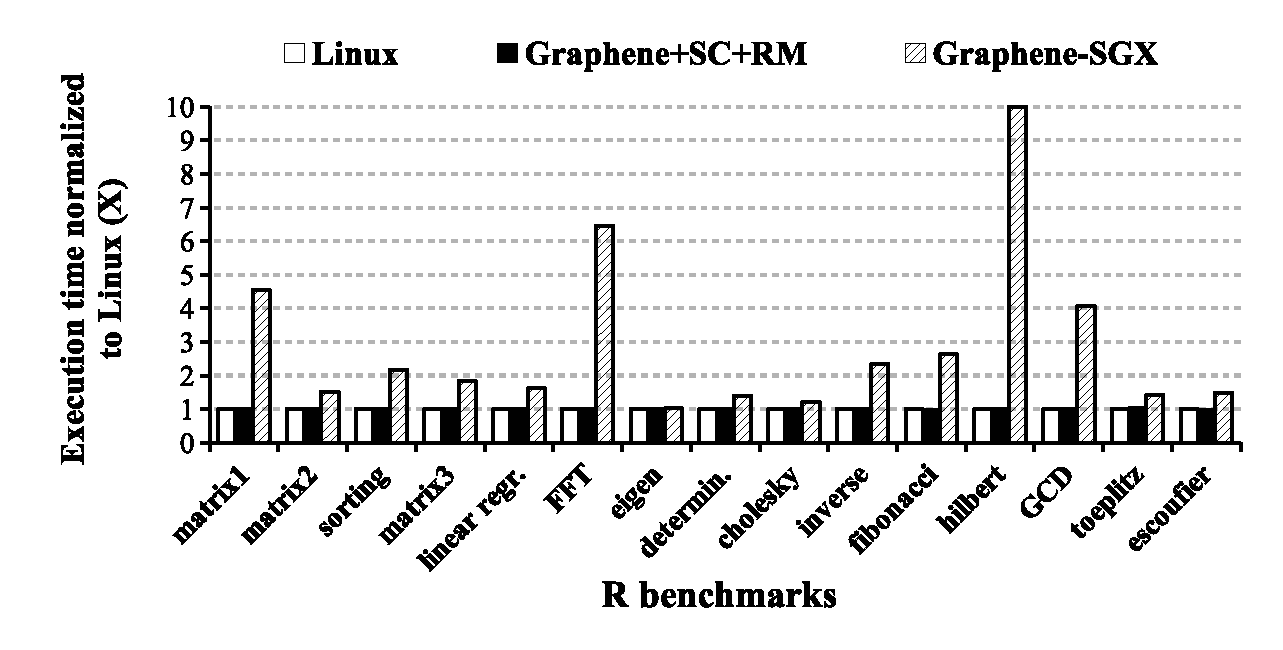
\includegraphics[width=\linewidth]{sgx/r-overhead}\\
{\bf (a) R}
\end{minipage}
\begin{minipage}{.275\textwidth}
\centering
\includegraphics[width=\linewidth]{sgx/gcc-overhead}\\
{\bf (b) GCC}
\end{minipage}
\begin{minipage}{.25\textwidth}
\centering
\includegraphics[width=\linewidth]{sgx/curl-overhead}\\
{\bf (c) CURL}
\end{minipage}

\caption{Performance overhead on desktop applications, including latency of R, execution time of GCC compilation, download time with CURL. The evaluation compares native Linux, \graphene{}, and \graphenesgx{}.} %{\bf Enclave creation time is deducted from the GCC execution time.}}
\label{fig:desktop-overhead}
\end{figure*}



\subsection{Command-Line applications}


We also evaluate the performance of a few commonly-used command-line applications.
%, to evaluate the performance of \graphenesgx{} on PCs instead of servers and clouds.
Three off-the-shelf applications are tested in our experiments:
{\bf R} (v3.2.3) for statistical computing~\cite{r-project}; {\bf GCC} (v5.4), the general GNU C compiler~\cite{gcc}; {\bf CURL} (v7.74), the default command-line web client on UNIX~\cite{curl}.
These applications are chosen because they are frequently used by Linux users,
and each of them potentially  be used 
in an enclave to handle sensitive data---either on a server or a client
machine.
% can realize profitable scenarios of using enclaves on desktop machines.



We evaluate the latency or execution time of these applications. 
%, because desktop users tend to care more about responsiveness than throughput.
In our experiments, both R and CURL have internal timing features to measure the wall time
of individual operations or executions.
%However, for other applications like GCC which does not include internal timing, evaluating the execution time can be influenced by many factors.
On a Linux host, the time to start a library OS is higher than a simple 
process, but significantly lower than booting a guest OS in a VM or
starting a container. 
Prior work measured Graphene (non-SGX) start time at 641 $\mu$s~\cite{tsai14graphene}, whereas starting an empty Linux VM takes 10.3s and starting a Linux (LXC) container takes 200 ms~\cite{agarwal15container}. 
%% dp; Note that this is MILLI seconds, not micro seconds.
%average memory footprint of an empty Linux VM, with memory deduplication, is about 96MB, . 


On SGX, the enclave creation time is relatively higher, \fixme{added more detailed number} ranging from 0.5s (a 256MB enclave) to 5s (a 2G enclave), which is a fixed cost that any application framework
will have to pay to run on SGX.
%For library OSes, the time for creating and initializing an enclave is not trivial, because it is similar to booting an lightweight OS.
% a significant part of the start-up time
% of an application is more significant, because creating enclaves is expensive.
%We consider the enclave creation time as a fixed cost for any application running in \graphenesgx{},
%and acceptable to users as long as it is responsive.
Enclave creation time is determined by the latency of the hardware and the Intel kernel driver, and is primarily a function of the size of 
the enclave, which is specified at creation time because it affects the enclave signature. %\fixmedp{although can't it grow with eadd?}.  
For non-server workloads that create multiple processes during execution,
such as GCC in Figure~\ref{fig:desktop-overhead},
the enclave creation contributes a significant portion to the execution time overheads, illustrated as a stacked bar.
%Since the enclave creation time is related to the enclave size, and unrelated to the workload,
%we deduct the enclave creation time from the execution time of GCC in Figure~\ref{fig:desktop-overhead}. \fixmedp{I think it might be better to show this as a stacked bar instead of just removing it.  Opaquely subtracting this cost doesn't seem right.  Let's discuss dp: I thought we agreed to change this...}

{\bf R}~\cite{r-project} is a scripting language often used for
data processing and statistical computation.
With enclaves, users can process sensitive data on an
OS they don't trust.
We use an R benchmark suite developed by Urbanek et al.~\cite{r-benchmark-25}, which includes 15 CPU-bound workloads such as matrix computation and number processing.
\graphenesgx{} slows down by less than 100\% on the majority of the workloads, excepts the ones which involve allocation and garbage collection: ({\tt matrix1} creates and destroys matrices, and both {\tt FFT} and {\tt hilbert} involve heavy garbage collection.)
Aside from garbage collection, these R benchmarks do not frequently interact with the host.
We further note that non-SGX \graphene{} is as efficient as Linux on all workloads, 
and these overheads appear to be SGX-specific.
%\fixmedp{Check this pontification}
In our experience, garbage collection and memory management code in managed language runtime
systems tends to be written with assumptions that do not match enclaves,
such as a large, sparse address space or that memory can be demand paged 
nearly for free (SGX version 1 requires all memory to be mapped
at creation); a useful area for future work would be to design
garbage collection strategies that are optimized for enclaves.
%we believe the overheads on \graphenesgx{} are contributed by enclaves.
 
{\bf GCC}~\cite{gcc} is a widely-used C compiler.
By supporting GCC in enclaves, developers can compile closed-source applications on customers' machines,
without leaking the source code.
GCC composes of multiple binaries, including {\tt cc1} (compiler), {\tt as} (assembler), and {\tt ld} (linker).
Therefore, GCC is a multi-process program using \syscall{execve}.
We test the compilation of thee source files with varied sizes,
using single C source files collected by MIT~\cite{gcc-benchmark}.
Each GCC execution typically \fixme{it's five, not four} creates five processes, and we run each process in a 256MB enclave by default.
%and has a fixed cost on enclave creation, which is unrelated to workload and depends on the enclave size.
%\fixme{check this}
\fixme{clarified this part, to prevent confusion between latency and overhead. also, GCC numbers got better.}
For a small workload like compiling {\tt gzip.c} (5 kLoC), running in \graphenesgx{} (4.1s) is 18.7$\times$ slower than Linux (0.2s).
The bulk of this time is spent in enclave creation, taking 3.0s in total, while the whole execution inside the enclaves, including initialization of the library OS and OS shield, takes only 1.1s, or 4.2$\times$ overhead.
For larger workloads like {\tt oggenc.c} (50 kLoC) and {\tt gcc.c} (500 kLoC), 
the overhead of \graphenesgx{} is less significant. % (3.6$\times$ and 2.1$\times$ overhead, respectively).
For {\tt gcc.c} (500 kLoC), we have to enlarge one of the enclaves ({\tt cc1}) to 2GB,
but running on \graphenesgx{} (53.1s) is only 2.1$\times$ slower than Linux (17.2s),
and 7.1s is spent on enclave creation.
%and the creation of four enclaves takes 8s.
%Each compilation has a fixed enclave creation time in \graphenesgx{}, which is about 1--2 seconds per enclave. We deduct the creation time of all enclaves  to gain more meaningful results, but do not hide rest of the overhead on fork.
%\fixmedp{Also not comfortable with this; add a bar?}
%In general, GCC in \graphenesgx{} is 1--5$\times$ slower than GCC on native Linux. 
%\fixmedp{This really needs some profiling if possible}
The overhead of non-SGX \graphene{} on GCC is marginal.
 



{\bf CURL}~\cite{curl} is a command-line  web downloader.
\graphenesgx{} can make CURL into a secure downloader that attests both server and client ends.
We evaluate the total time to download a large file, ranging from 1MB to 1GB, from another machine running Apache. % over Gigabit LAN.
%across high-speed university network\fixmedp{more specific, as above}.
\graphene{} has marginal overhead on CURL, and
\graphenesgx{} adds 7--61\% overhead to the downloading time of CURL, due to the latency of I/O.


\begin{figure*}[t!]
\centering

\begin{minipage}{.3\textwidth}
\centering
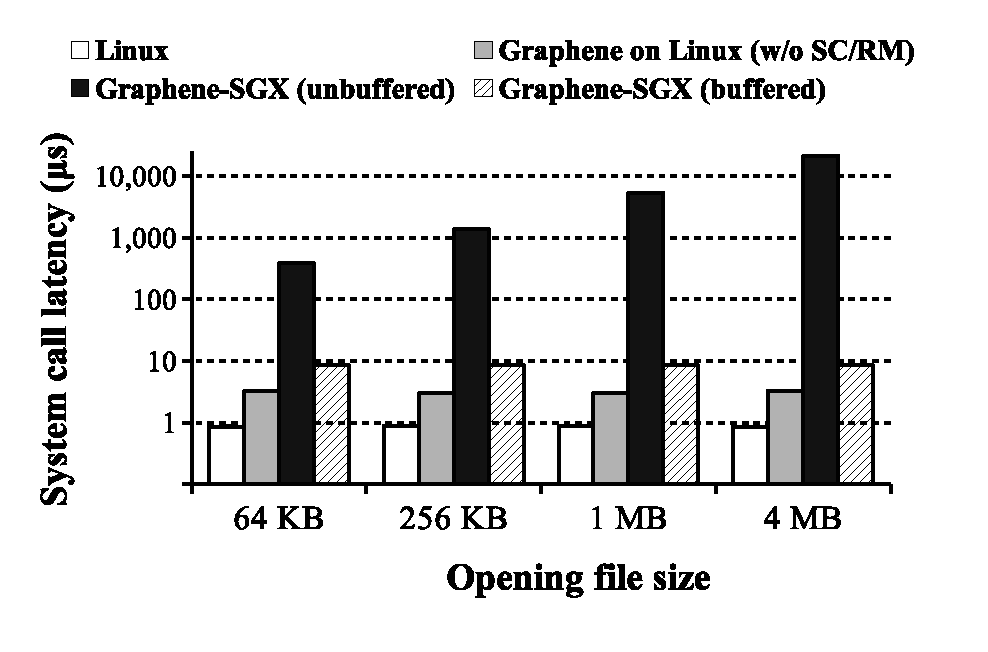
\includegraphics[width=\linewidth]{sgx/open-latency}\\
{\bf (a) Open a file}
\end{minipage}
\begin{minipage}{.3\textwidth}
\centering
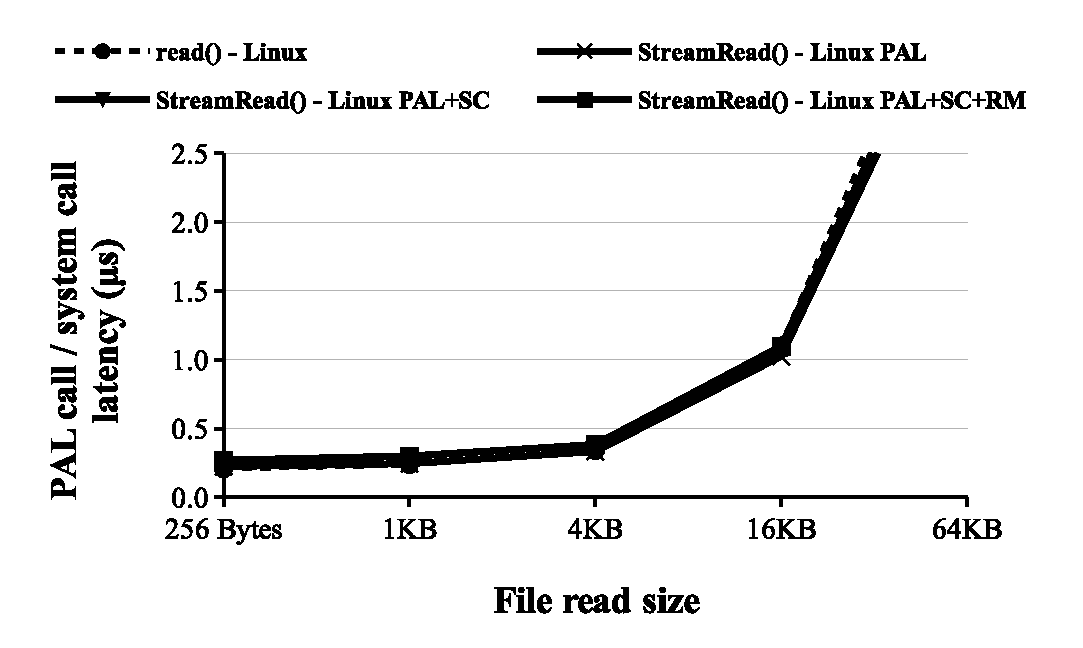
\includegraphics[width=\linewidth]{sgx/read-latency}\\
{\bf (b) Read a file}
\end{minipage}
\begin{minipage}{.3\textwidth}
\centering
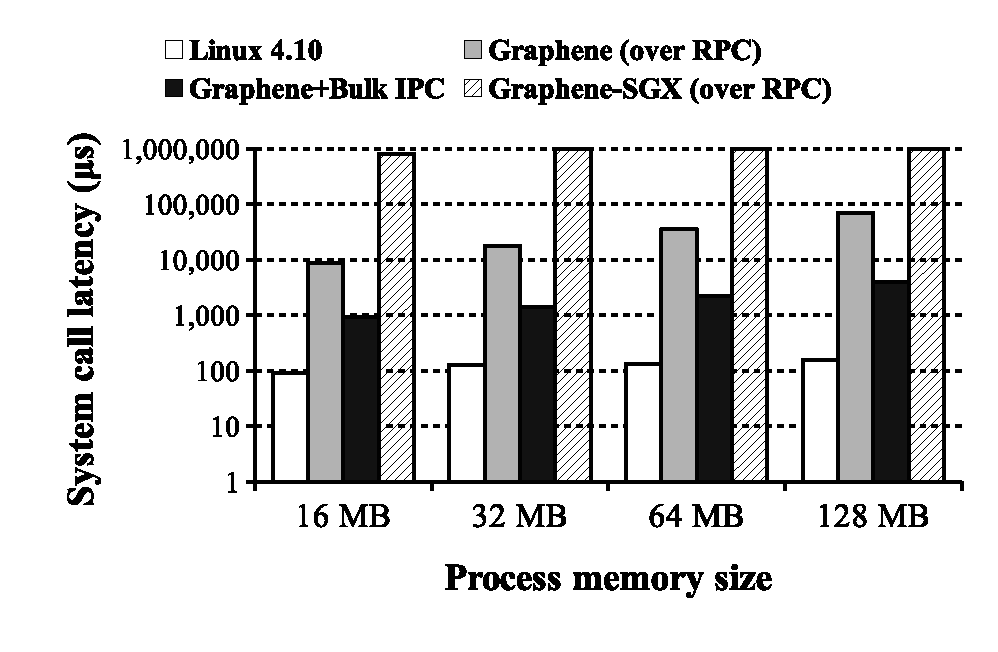
\includegraphics[width=\linewidth]{sgx/fork-latency}\\
{\bf (c) Fork a process}
\end{minipage}

\caption{Latency of some expensive system calls in \graphenesgx{}, including opening and reading a secured (authenticated) file, and forking a new process. The results are compared with native Linux and \graphene{}.}
\label{fig:syscall}
\end{figure*}


\subsection{Performance Overhead Analysis}


In this section we evaluate a few system operations that are heavily impacted by the \graphenesgx{} design.
%To shield dynamic loading and process creation,
%\graphenesgx{} uses computationally-expensive cryptographic techniques \fixmedp{more specific?} to verify enclave inputs.
% under the circumstance that the host OS cannot be trusted.
%As a trade-off to the security, the performance will be affected
%by additional cryptographic computation.
We measure the \syscall{open}, \syscall{read}, and \syscall{fork} system calls
using LMbench 2.5~\cite{McVoy:lmbench}.
A primary source of the overheads on these system calls is the cost of shielding applications, with run-time checks on the inputs.
Cryptographic techniques are used to: (1) validate the file against the secure hash, at \syscall{open}, (2) check the file chunks against the Merkle tree, at \syscall{read}, and (3) establish a TLS connection over inter-enclave RPC, at \syscall{fork}.
%opening a integrity-sensitive file for the first time, 
% or using cryptographic techniques, such as secure hashing, to verify the inputs.
% microbenchmarking specific system calls: 
% system calls,
%with different application settings.
%The microbenchmark is part of the LMBench 2.5 test suite
%\fixmedp{maybe merge this in the above paragraph, which feels a little coy}
%For instance, in order to shield dynamic loading, \graphenesgx{} checks each binary file against the secure hashes in the manifest,
%when the file is opened for the first time---after the whole file is copied into the enclave.
%\fixmedp{This happens after they are copied into enclave, memory right?}
%The verification happens when opening the file for the first time (often by the 
%After \graphenesgx{} validates the file, we generate a series of hashes of the file in chunks, as a merkle tree.
%to prevent verifying the whole file again when later randomly reading a part of the file.
%\fixmedp{So is this for the case when a file is swapped out?  I'm confused here - some details are missing}
%The latency of opening and reading an authenticated file in \graphenesgx{} is dominated by SHA256 and SHA512 calculation.
The remaining overheads contribute to exiting the enclave for host system calls, and bringing memory into the EPC (enclave page cache) or decrypting 
memory on a last-level cache miss. %and later the cache where the memory is decrypted by the CPU.


Figure~\ref{fig:syscall}(a)
shows the overhead for authenticating files in \syscall{open}.
\fixme{change overhead to latency}
Depending on the file size, the latency of \syscall{open} on \graphenesgx{} is 383$\mu$s (64KB file) to 21ms (4MB file), whereas on Linux, the latency is constant at 0.85$\mu$s.
We note that this is where enclaves are at a disadvantage, as \syscall{open} 
normally does not need to read file content; whereas here \graphenesgx{} uses \syscall{open}
as a point at which to validate file content.
For a subsequent \syscall{open}, when the Merkle tree is already generated, the overhead of simply exiting enclave for \syscall{open}, and searching the file list in the manifest, is about 9$\times$.
%\fixmedp{why?}


One might be able to optimize further for cases where only part of a file is accessed
with incremental hashing.  However, in the common case where nearly all of the file is accessed,
these costs are difficult to avoid when host file system is untrusted.
Another opportunity 
is to create the Merkle tree offline, when the manifest is created.
%\fixmedp{I think the second idea has legs...}


%This is an inevitable cost, because normal \funcname{open} on trusted OSes
%need not to access file content.
%After verifying the file, \graphenesgx{} buffers the chunk hash values, to skip whole-file verification when the file is reopened.

Figure~\ref{fig:syscall}(b)
shows the overhead for authenticating files in \syscall{read}, which 
is lower than \syscall{open}.
Since the whole file has been verified at \syscall{open}, the sequential \syscall{read} only verifies the chunks of files it is reading from untrusted memory.
%Reads from data cached in enclave memory are cheaper.  %\fixmedp{right? can we say how much cheaper?  Maybe add separate bars for both cases?}
% Therefore, \syscall{read} is actually much cheaper than \syscall{open}.
Depending on the size of blocks being read, the latency on \graphenesgx{} is 0.5$\mu$s (64-byte \syscall{read}) to 16.9$\mu$s (4KB \syscall{read}). The latency of \syscall{read} on Linux is \roughly{}0.1$\mu$s for any block size below 4KB.
If the file is not authenticated,
\graphenesgx{} only copies the file contents into the buffer, and the overhead reduces to 48\% (64-byte \syscall{read}) to 83\% (4KB \syscall{read}).
\fixmedp{Consider doing larger buffers, say up to 64k or even 4 MB}

%\fixmedp{In the legend for 7b, unsecure should be insecure}


Figure~\ref{fig:syscall}(c) shows the overhead of forking a process.
As described in \ref{sec:multiproc}, the latency of \syscall{fork} in \graphenesgx{} is affected by three factors:
creation of a new enclave, local attestation of the integrity, and duplicating the process state over an encrypted RPC stream.
Combining these factors, \syscall{fork} is one of the most expensive calls in \graphenesgx{}.
%, but at least it is supported natively on the current hardware.
The default enclave size is 256MB.
%which takes \roughly{}0.5s to create. 
Our evaluation shows that the latency of forking a process is around 0.8s (16MB process) to 2.7s (128MB process), but can be more expensive if the parent process uses more memory.
The trend matches the performance of \graphene{} without the bulk IPC optimization.
\fixmedp{If you want, some thoughts on how this might be improved in the future would be nice...  One good suggestion is recycling enclaves, or pre-forking so measurements can be done in parallel}
%Due to the overhead on \funcname{fork}, \graphenesgx{} is not suitable for fork-intensive workloads like Bash scripts
%if performance is critical.

\fixme{talk about a limitation of improving fork. check this.}
One way to further optimize \syscall{fork} is to reduce or avoid enclave creation time; one can potentially pre-launch a child enclave, and then migrate the process contents later when \syscall{fork} is called.
There might be another opportunity to improve the latency of process migration,
if copy-on-write sharing of enclave pages can be supported in future generations of SGX.
%Unfortunately, sending the process contents is difficult to avoid in \syscall{fork},
%as SGX disallows sharing enclave memory between multiple enclaves.

%\fixmedp{I assume 5.4 isn't done yet}



\subsection{TCB Size and Shielded Functionality}

In this section we measure the increase in TCB size of \graphenesgx{},
%in lines of code, 
as well as 
%compare the TCB size increased by \graphenesgx{} to an unmodified application, in lines of code, and 
the OS functionality shielded by the framework.
We compare to \scone{} and \panoply{}, using
%For SCONE and Panoply, we use 
numbers reported in their papers. 
%The conventional One generally assumes 
A smaller TCB is generally easier to review or possibly verify,
and is assumed to have fewer vulnerabilities.
%more implies lower burden for code review or formal verification, and less risk of writing exploitable code.
%For instance, Panoply argues that, because its use cases are typically smaller than 20kLoC, including both the application logic and Panoply itself, it is within the realm of future, automated verification~\cite{shinde17panoply}.

\fixmedp{Reviewer B asks for memory footprint, which isn't a bad idea}

\begin{table}
\footnotesize
\centering
\bgroup
\def\arraystretch{1.2}
\setlength{\tabcolsep}{0.5em}
\begin{tabular}{>{\raggedright\arraybackslash}p{9em}>{\raggedleft\arraybackslash\bf}p{7em}>{\raggedleft\arraybackslash}p{4.25em}>{\raggedleft\arraybackslash}p{4.25em}}
Components                    & \graphenesgx{}  & \scone{}     & \panoply{}  \\
\hline
libc (ld, libm, pthread)      &  1,292 &   88 & --      \\
                              & (glibc-2.19) & (musl)   &          \\
Library OS                    &     34 &  --      & --     \\
PAL / OS Shield               &     22 &   99 & 10  \\
\hline
Total                         &  1,348 &  187 & 10  \\
\hline
\end{tabular}
\egroup
\caption{TCB size (in thousands of lines of code) of \graphenesgx{}, \scone{}, and \panoply{}.}
\label{tab:tcb-size}
\end{table}

Table~\ref{tab:tcb-size} lists the lines of code in each components within the TCB of \graphenesgx{}, \scone{}, and \panoply{}.
By comparing the total TCB size, \graphenesgx{} is 9$\times{}$ larger than \scone{}, and 134$\times{}$ larger than \panoply{}.
However, the primary difference is the selection of libc: 
for maximum compatibility, \graphene{} uses glibc.
\scone{} uses the smaller musl libc, which lacks some features of glibc.
%it would be easy to use the smaller, and incomplete, musl libc.
%SCONE uses 
% Linux applications, \graphenesgx{} chooses to use a minimally-modified glibc, whereas SCONE uses the much more lightweight musl and 
\panoply{} excludes libc from its TCB,
% \fixmedp{what is their rationale, again? Check this}
to fit into the range of automated formal verification,
as they shield at the libc interface.
In principle, \graphene{} could easily support musl as well as glibc for applications
that do not need the additional features of glibc.
We also see the benefit of removing unused code from 
libraries, especially in an unsafe language,
similar to the approach taken in unikernels~\cite{unikernels}.
On balance, 
this choice of libc implementation is largely orthogonal to the issue
of how general-purpose the shields are.

%We argue that the choice of libc is orthogonal to the design of \graphenesgx{}; one can statically compile the applications against musl or glibc if TCB size is a concern, or given plenty of time, trim the libc functionality to bare minimum. 

If we focus on the TCB size of the library OS and the shields, 
\graphenesgx{} is 
%library OS and PAL in \graphenesgx{}, with the shielding layer of SCONE, we are 
44\% smaller than \scone{}. 
We cannot analyze the size of \scone{} because it is closed source.
%, although
%we suspect
%Although it is unclear what is in the implementation of SCONE, because it is not yet open-sourced, we believe the largest portion of their TCB contributes to the cryptography library.
\panoply{} has a smaller TCB in its shield, but within the same order of magnitude.
Panoply only shields 91 out of 256 supported POSIX functions; for context, POSIX 1003.1 defines 1,191 APIs~\cite{POSIX1003-1-2008}.
%out of 256 currently supported by \panoply{} \fixmedp{The better number is how many total functions in POSIX}.

All three of these compatibility layers or shields are within the same
order of magnitude in code size, and the differences are likely 
correlated with different ranges of supported functionality.
A recent study indicates that only order-of-magnitude differences in code
size correlate with reported CVE vulnerabilities; within the same order-of-magnitude,
the data is inconclusive that there is a meaningful difference in risk~\cite{security-metric}.
Thus, increased generality does not necessarily come with 
increased risk. % is not a clear relationship between risk 

% data only correlates
%with differences in code size when 

%Besides the choice of libc, we argue that the TCB size of a library OS or a shim shielding layer is actually correlated with the functionality that it supports or shields. Because none of the three frameworks have completely shielded the whole Linux system call table or POSIX, it is unclear how much code has to be added in the future. \graphenesgx{} also shows that one can always engineer a library OS with a small TCB, if most code is not reused from a monolithic OS kernel like Windows or Linux.
%A recent study of the CVE database also points out that having a larger TCB does not necessarily indicate more vulnerabilities, even when the difference is more than two order-of-magnitude. 



\input{apistudy}

\makeatletter
\def\input@path{{}}
\makeatother
\graphicspath{{}}
\section{Conclusion}

This paper demonstrates that the costs of running an unmodified application in SGX on a library OS are
marginal compared to thinner shims.
The major costs of using SGX are still hardware limitations of SGX.
As SGX and similar technologies mature, these design choices may have more impact.
In the interim, \sysname{} serves as a simple, open-source tool to quickly bring up
existing applications on SGX, and then incrementally adapt the code to improve performance and security on SGX.
%\fixme{Mona suggests dropping this}
%We believe the \sysname{} design is sufficiently general that porting applications to AMD's PSP
%features should only require porting the PAL.
%\fixme{Mona suggest adding this argument:
%``Graphene-SGX can provide support for running unmodified applications on SGX that provide encryption and integrity Vs SEV that can run unmodified applications, but provides only encryption but no integrity guarantees.''}


\newpage
\phantomsection
\addcontentsline{toc}{chapter}{References}
\renewcommand{\bibname}{\centerline{\normalsize\bf{References}}}
\bibliographystyle{plainnat}
\bibliography{../bibliography}

\newpage
\begin{appendices}
\chapter{Formal Definitions of \UsageMetric{} and \CompatMetric{}}
\label{chap:defs}

%\fixmedp{The formal definition of importance in section 2.1 is hard to follow, in part because of the naming. The names of variables (Dependentapi, inst) don't make clear the types of the variables (a package, set of packages, set of API, instance, set of instance) etc. It would be helpful to reconsider the terminology to make the variable types more clear.
%In the equations in 2.2, explaining what E means would be helpful, as it is not obvious from the context. Also, should Weighted Compliance be a function of the instance in addition to the API?
%}

\section{\UsageMetric{} --- A Metric for APIs}
\label{sec:defs:usagemetric}

\vspace{0.1in}
{\noindent
\fbox{\begin{minipage}{\linewidth}
\setlength{\parindent}{-0.1in}
\setlength{\leftskip}{0.1in}
\setlength{\rightskip}{0.1in}
 Definition: {\bf \UsageMetric{}.} \\
For a given API, the probability that an installation includes
at least one application requiring the given API.
%at least one broken application
%(whose API footprint covers the target API),
%if the target API was removed.
\end{minipage}}}
\vspace{0.1in}

A system installation ($\mathtt{inst}$)
is a set of packages installed ($\{\mathtt{pkg}_1, \mathtt{pkg}_2, ..., \mathtt{pkg}_k \in \mathtt{Pkg}_\mathtt{all}\}$).
For each package ($\mathtt{pkg}$)  that can be installed by the installer,
we analyze every executable included in the package 
($\mathtt{pkg} = \{\mathtt{exe}_1, \mathtt{exe}_2, ..., \mathtt{exe}_j\}$), and
generate the API footprint of the package as:
\begin{align*}
{\mathtt{Footprint}}_{\mathtt{pkg}} = \{\mathtt{api} \in {\mathtt{API}}_{\mathtt{all}} \mid \text{\parbox{2.3in}{$\exists \mathtt{exe} \in \mathtt{pkg}$,
$\mathtt{exe}$ has usage of $\mathtt{api}$}}\}
\end{align*}

\noindent
For a target API, \usagemetric{} is calculated as the probability
that any installation includes
at least one package that uses the API;
i.e.,
the API belongs to the footprint of at least one package.
Using \osdist{}'s package installation statistics, one can calculate the
probability that a specific package is installed as:
\begin{align*}
Pr\{\mathtt{pkg} \in \mathtt{Inst}\} = \frac{\text{\# of installations including $\mathtt{pkg}$}}{\text{total \# of installations}}
\end{align*}

\noindent
Assuming the packages that use an API are  
$\mathtt{Dependents}_\mathtt{api} = \{\mathtt{pkg}|\mathtt{api} \in \mathtt{Footprint}_\mathtt{pkg}\}$.
\Usagemetric{} is the probability that at least one package
from $\mathtt{Dependents}_\mathtt{api}$ is installed on a random installation, which is calculated as follows:
\begin{align*}
&\mathtt{Importance}(\mathtt{api}) = Pr\{\mathtt{Dependent}_\mathtt{api} \bigcap \mathtt{Inst} \neq \emptyset\} \\
&= 1 - Pr\{\forall \mathtt{pkg} \in \mathtt{Dependent}_\mathtt{api}, \mathtt{pkg} \notin \mathtt{Inst}\} \\
&= 1 - \prod_{\mathtt{pkg} \in \mathtt{Dependent}_\mathtt{api}} Pr\{\mathtt{pkg} \notin \mathtt{Inst}\} \\
&= 1 - \prod_{\mathtt{pkg} \in \mathtt{Dependent}_\mathtt{api}} (1 - \frac{\text{\# of installations including $\mathtt{pkg}$}}{\text{total \# of installations}})
\end{align*}

\section{\CompatMetric{} --- A System-Wide Metric}
\label{sec:defs:compatmetric}

%% An accurate metric for API compatibility must take into account at least two factors:
%% \begin{compactenum}
%% \item For each interface in the API, what are the applications that rely on it and could be affected if the interface is removed? ({\em application footprint})
%% \item For each application, how many installations of the system in the world has included it? ({\em application popularity})
%% \end{compactenum}


%% \fixmedp{Term for each call, vs system overall: API Importance and Effective Coverage?}

%% To accurately evaluate compatibility, we design a metric that is quantifiable, \fixmetsai{one more word here}, and easy to interpret.

\begin{comment}
We defined {\bf platform compatibility} as "{\em the probability of porting any installation of an OS distribution onto the target OS without any effort}".
The definition of an {\em installation} is a combination of application setup on a standalone OS instance.
An Installation can exist on physical machines,
or any machines of generalized sense such as a virtual machines, containers or subsystems.
In our model, installations represent customers of the OS, who are considered equal when providing any services.
\end{comment}

\vspace{0.1in}
%\fixmetsai{Find a good name for our metric} 
{\noindent
\fbox{\begin{minipage}{\linewidth}
\setlength{\parindent}{-0.1in}
\setlength{\leftskip}{0.1in}
\setlength{\rightskip}{0.1in}
Definition: {\bf \CompatMetric{}.} \\
For a target system, the fraction of applications supported,
weighted by the popularity of these applications.
\end{minipage}}}
\vspace{0.1in}

\Compatmetric{} is used to evaluate the relative compatibility on a system that
supports a set of APIs ($\mathtt{API}_\mathtt{Supported}$).
For a package on the system, we define it as supported if 
if every API that the package uses is in the supported API set.
In other words, a package is supported if it is a member of the following set:
\begin{align*}
\mathtt{Pkg}_\mathtt{Supported} = \{\mathtt{pkg} | \mathtt{Footprint}_\mathtt{pkg} \subseteq \mathtt{API}_\mathtt{Supported}\}
\end{align*}

\noindent
Using \compatmetric{}, one can estimate the fraction of packages in an installation that end-users can expect a target system to support.
For any installation
that is an arbitrary subset of available packages
($\mathtt{Inst} = \{\mathtt{pkg}_1, \mathtt{pkg}_2, ..., \mathtt{pkg}_k\} \subseteq \mathtt{Pkg}_\mathtt{all}$),
\compatmetric{} is the expected value of
the fraction in any installation ($\mathtt{Inst}$)
that overlaps with the supported packages ($\mathtt{Pkg}_\mathtt{Supported}$):
\begin{align*}
\mathtt{Weighted Completeness}(\mathtt{API}_\mathtt{Supported}) =
E(\frac{|\mathtt{Pkg}_\mathtt{Supported} \bigcap \mathtt{Inst}|}{|\mathtt{Inst}|}) 
\end{align*}
where $E(\mathtt{X})$ is the expected value of $\mathtt{X}$.

Because we do not know which packages are installed together,
except in the presence of explicit dependencies,
%Lacking of the distribution data of each package, we approximate the value of \compatmetric{}
%by ignoring {\em higher order} estimators
%of the expectation, assuming events of installing each package to be independent.
we assume package installation events are independent.
Thus, the approximated value of \compatmetric{} is:
\begin{align*}
\frac{E(|\mathtt{Pkg}_\mathtt{Supported} \bigcap \mathtt{Inst}|)}{E(|\mathtt{Inst}|)}
\sim \dfrac{\sum_{\mathtt{pkg} \in \mathtt{Pkg}_\mathtt{Supported}} (\dfrac{\text{\# of installations including $\mathtt{pkg}$}}{\text{total \# of installations}})}{\sum_{\mathtt{pkg} \in \mathtt{Pkg}_\mathtt{all\hspace{0.21in}}} (\dfrac{\text{\# of installations including $\mathtt{pkg}$}}{\text{total \# of installations}})}
\end{align*}

\end{appendices}

\end{document}
